\documentclass[conference]{IEEEtran}

\usepackage{array}

\usepackage{textcomp}

\usepackage{url}
\usepackage{verbatim}
\usepackage{graphicx}
\usepackage{cite}
\hyphenation{op-tical net-works semi-conduc-tor IEEE-Xplore}
% updated with editorial comments 8/9/2021

\usepackage{booktabs}
\usepackage{todonotes}
\usepackage{amsmath,amssymb,amsthm}
\usepackage{graphicx}
\usepackage{caption}
\usepackage{subcaption}
\usepackage{enumitem}
% \usepackage{natbib}
\usepackage{algorithm}
\usepackage{algpseudocode}
\algrenewcommand\algorithmicfunction{\textbf{Function}}
% \makeatletter
% \renewcommand{\ALG@name}{Function} % keep keyword
% \algrenewtext{Function}[2]{\algorithmicfunction\ #1(#2)} % #1 = name, #2 = args
% \makeatother

\newcommand{\ICall}[2]{\textproc{#1}(#2)}
\renewcommand{\textproc}[1]{\textnormal{#1}} % preserve case


\usepackage{hyperref}
\usepackage[capitalise,nameinlink]{cleveref}
\crefname{figure}{Fig.}{Figs.}
\Crefname{figure}{Fig.}{Figs.}
\crefname{table}{Table}{Tables}
\Crefname{table}{Table}{Tables}
\crefname{equation}{Eq.}{Eqs.}
\Crefname{equation}{Eq.}{Eqs.}
\crefname{algorithm}{Alg.}{Algs.}
\Crefname{algorithm}{Alg.}{Algs.}
\crefname{section}{Section}{Sections}
\Crefname{section}{Section}{Sections}
\crefname{appendix}{Appendix}{Appendices}
\Crefname{appendix}{Appendix}{Appendices}

% \usepackage[linesnumbered,ruled,vlined]{algorithm2e}
% correct bad hyphenation here

\newcommand{\frwork}{PaTAS}
\newcommand{\frworkfunc}{PTAF}
\newcommand{\pf}{\mathit{Pf}}
\newcommand{\supp}{Supplementary Materials }
\newcommand{\suppp}{Supplementary Materials}

\newtheorem{theorem}{Theorem}
\newtheorem{definition}{Definition}
\newtheorem{lemma}{Lemma}
\newtheorem{proposition}{Proposition}
\newtheorem{corollary}{Corollary}

\theoremstyle{remark}
\newtheorem{remark}{Remark}

\theoremstyle{definition}
\newtheorem{example}{Example}

\setlength{\textfloatsep}{5pt plus 1pt minus 1pt}
\setlength{\dbltextfloatsep}{6pt plus 1pt minus 1pt}
\setlist{noitemsep,topsep=2pt,leftmargin=*}
\captionsetup{font=footnotesize,skip=4pt}
\begin{document}

\title{PaTAS: A Framework for Trust Propagation in Neural Networks Using Subjective Logic}

% \author{Koffi Ismael Ouattara,
%         Ioannis Krontiris, 
%         Theo Dimitrakos,
%         Dennis Eisermann,
%         Houda Labiod,
%         and Frank Kargl }

\maketitle

\begin{abstract}
Trustworthiness has become a key requirement for deploying artificial intelligence in safety-critical applications, yet conventional metrics such as accuracy and precision fail to capture uncertainty or the reliability of predictions, particularly under adversarial or degraded conditions. This paper introduces the \emph{Parallel Trust Assessment System (PaTAS)}, a framework for modeling and propagating trust in neural networks using Subjective Logic (SL). PaTAS operates in parallel with standard neural computation through \emph{Trust Nodes} and \emph{Trust Functions} that propagate input, parameter, and activation trust across the network. It defines a \emph{Parameter Trust Update} mechanism that refines parameter reliability during training and an \emph{Inference-Path Trust Assessment (IPTA)} that, given a trained model and an input, returns a trust opinion, quantifying belief, disbelief, and uncertainty, on the prediction. Experiments on real-world and adversarial datasets show that these estimates are interpretable, symmetric, and convergent, and that they complement accuracy: PaTAS assigns markedly lower trust to outputs from adversarially patched inputs and flags predictions that remain accurate yet rely on parameters learned from corrupted data, reliability gaps that confidence scores do not reveal. Against maximum-softmax, MC~Dropout, and Evidential Deep Learning baselines, PaTAS detects out-of-distribution inputs (AUROC 0.975 vs.\ at most 0.936) and corrupted inputs that confidence-based methods rank near chance (0.97 vs.\ 0.63), flags training-label corruption without any test data, and self-diagnoses per dataset whether input-level trust is informative. PaTAS thereby provides a foundation for transparent, quantifiable trust reasoning across the AI lifecycle.
\end{abstract}

% \begin{IEEEkeywords}
% Trustworthy AI, Subjective Logic, Neural Networks, Uncertainty Quantification, Trust Propagation, Data Corruption
% \end{IEEEkeywords}

% =====================================================================
% Author working notes (kept out of the PDF).
%
% DONE (2026-08-17): Experiment 4 (comparative evaluation) written in
%   sections/evaluation.tex with final cluster numbers — OOD + corruption
%   detection (tab:comparative), input-trust ablation row, applicability
%   diagnostics (tab:diagnostics), training-quality audit (tab:audit).
%   Abstract + conclusion updated accordingly.
% Remaining before submission:
%   - Compile on Overleaf and check the 10-page budget; if over, first
%     candidates to trim: Exp-1 intermediate-scenario enumerate,
%     Implementation Details paragraph, Exp-3 prose (tables carry it).
%   - Optional: epsilon/fusion ablation numbers exist in the results
%     archive (Ablation_* dirs) if a reviewer asks.
%   - Justify the gradient-trust assumption.
%   - Input/label trust availability: consider submitting the dataset
%     trust paper first so it can be cited rather than assumed.
% =====================================================================

\vspace{-0.5em}
\section{Introduction}

Artificial Intelligence (AI) systems, particularly Neural Networks (NNs), are employed in critical sectors such as healthcare, to interpret clinical images, or autonomous driving, to recognize elements in traffic scenes. While highly performant, they often operate as black boxes offering limited insight into the reliability of their outputs, an opacity that becomes critical under adversarial, uncertain, or degraded conditions. Conventional metrics such as accuracy or precision do not capture uncertainty or reliability and can mislead decision-makers~\cite{10.1145/3290605.3300509}: a model may report 95\% accuracy while being evaluated on mislabeled data, unaccounted for dataset bias, label noise, or adversarial corruption. Reliability measures must therefore go beyond predictive confidence and consider the quality and provenance of inputs, the reliability of training data, and the fit of learned parameters.

As AI systems become integral to critical applications, \emph{trustworthiness} has emerged as a fundamental requirement. A trustworthy system must be lawful, ethical, and robust~\cite{ec2019ethics}, some of which translate into measurable properties such as accuracy, robustness, fairness, and explainability~\cite{10.3389/fdata.2024.1467222}. Embedding these across the AI pipeline, from data collection to deployment, is essential for preventing failures caused by poor data quality, bias, or unstable training. 

Despite this growing awareness, most models still provide limited mechanisms for representing confidence in their outputs. Trained under the assumption of clean, unambiguous labels, neural networks produce predicted probabilities that reflect similarity to seen patterns rather than genuine uncertainty, and that presuppose clean, in-distribution inference inputs; these assumptions are rarely satisfied in real-world or adversarial settings, where data quality, distributional shift, and how well parameters are learned all influence prediction reliability. Existing approaches, including attribution-based methods such as SmoothGrad~\cite{smilkov2017smoothgradremovingnoiseadding}, thus lack mechanisms to evaluate how trustworthiness in training inputs, activations, and parameters jointly affects output reliability. This gap motivates tools that reason explicitly about trustworthiness across the entire model lifecycle.

\paragraph*{Problem Statement}
Existing methods for trustworthiness and uncertainty estimation in neural networks face three key limitations. They \emph{neglect data provenance and quality}, assuming the training data are fully reliable; they offer only \emph{limited holistic propagation}, assessing reliability at the output layer alone; and they \emph{lack interpretability}, rarely yielding estimates that are both faithful to the model's reasoning and understandable to end users. Together these hinder reliable trustworthiness assessment in safety-critical or adversarial contexts.

\paragraph*{Contributions}
To address these challenges, we propose the \emph{Parallel Trust Assessment System (PaTAS)}, a framework for modeling and propagating trustworthiness in NNs using Subjective Logic (SL). Our contributions are:
\begin{enumerate}
    \item \emph{Parallel Trust Computation:} \textit{Trust Nodes} and \textit{Trust Functions} mirroring neural computations, propagating trust during training and inference through SL discounting and fusion.
    \item \emph{Parameter Trust Update:} an algorithm deriving trust in learned parameters from gradient values, input trust, and label trust, aligned with the learning dynamics.
    \item \emph{Inference-Path Trust Assessment (IPTA):} a context-aware trust function using activation-path information for per-instance trust scores.
    \item \emph{Empirical Validation:} evaluation on real-world and adversarial datasets showing interpretable trust estimates that expose reliability gaps under poisoned, biased, and uncertain data.
\end{enumerate}


% \section{Uncertainty in Neural Networks }

\vspace{-0.5em}
\section{Background}\label{sec:back}
Trust assessment in NNs requires a formalization that can represent ambiguity, inadequate evidence, and source reliability. This section summarizes Subjective Logic (SL) and its opinion representation (\cref{sec:backsl}), the main SL reasoning operators (\cref{sec:backslop}), and their application to dataset trustworthiness (\cref{sec:backtwdt}).
\vspace{-0.5em}
\subsection{Subjective Logic Fundamentals}\label{sec:backsl}
Classical probability theory models aleatoric uncertainty but cannot represent missing knowledge (ignorance) or contradictory information, which often arises from noisy or biased data. Subjective Logic~\cite{josang2016subjective} extends Dempster–Shafer theory~\cite{dempster1967upper,shafer1976mathematical} by representing trust as opinions whose belief and uncertainty are separate components, thereby distinguishing epistemic from aleatoric uncertainty.

A subjective opinion denoted by \(\omega_X^A\) expresses the beliefs of an agent \(A\) (e.g., a sensor, a human, or an external observer of a process) about states of a variable $X$ which takes its values from a domain $\mathbb{X}$ (i.e., a state space). A special case of a subjective opinion is a subjective binomial opinion where $card(\mathbb{X})=2$. For a binary variable $X \in \mathbb{X} = \{x, \overline{x}\}$, a binomial opinion is expressed as a quadruple:
\vspace{-0.5em}
\begin{equation}
\omega_x = \omega_{X=x} = (b_x, d_x, u_x, a_x)
\end{equation}
satisfying $b_x + d_x + u_x = 1$, where $b_x$ denotes belief in $x$, $d_x$ disbelief in $x$ (belief in \(\overline{x}\)), $u_x$ the uncertainty mass, and $a_x$ the base rate (prior probability of $x$ in the absence of evidence). Its projected probability is defined as:
\vspace{-0.5em}
\begin{equation}
P(x) = b_x + a_x u_x.
\label{eq:projected_prob}
\end{equation}
This projection reduces an opinion to an equivalent classical probability, enabling compatibility with standard probabilistic reasoning.

Binomial opinions can be derived from evidence: with $r_x$ and $s_x$ the amounts of positive and negative evidence for $x$, this work uses \emph{Baseline-Prior Quantification},
\begin{align}
b_x &= \frac{r_x}{W + r_x + s_x}, \quad
d_x = \frac{s_x}{W + r_x + s_x}, \quad
u_x = \frac{W}{W + r_x + s_x}
\label{eq:q1}
\end{align}
where the weight \(W>0\) guarantees residual uncertainty. Evidence-weighted and constant-uncertainty quantification~\cite{10.1007/978-3-032-19096-3_17} are alternatives that scale or fix the uncertainty mass instead.

A subjective opinion is meaningful only relative to a property under evaluation (e.g., accuracy or bias). In this work, trust is represented as a subjective binomial opinion $(t, d, u)$, where $t$ denotes trust (belief), $d$ distrust (disbelief), and $u$ uncertainty; the operators that make these opinions operational are introduced next.

\vspace{-0.5em}
\subsection{Subjective Logic Operators}\label{sec:backslop}

SL provides three families of reasoning operators for manipulating opinions~\cite{8009820,10706345,josang2016subjective}, all used in this work.

\begin{definition}[SL Operators]\label{def:fusion}
Let \(A\) be an agent reasoning about a variable \(X\).

\emph{Fusion} combines opinions held by two sources \(P\) and \(Q\) about the same proposition, \(\omega^A_{x} = \omega^P_{x} \oplus \omega^Q_{x}\); the appropriate variant (consensus, averaging, weighted, or cumulative) depends on whether the sources are correlated or independent.

\emph{Trust discounting} propagates an opinion along a referral chain: if \(A\) holds referral trust \(\omega^A_B\) in \(B\), who holds \(\omega^B_x\), then \(\omega^{[A;B]}_{x} = \omega^A_B \otimes \omega^B_{x}\), so that evidence from a partially reliable source is weakened and its uncertainty increased.

\emph{Inferential operators} generalize Bayesian reasoning through a conditional opinion \(\omega^A_{Y \mid X}\): \emph{deduction} derives \(\omega^A_Y\) from \(\omega^A_X\), and \emph{abduction} derives \(\omega^A_X\) from \(\omega^A_Y\).
\end{definition}
\noindent Details, summaries, and symbols for all operators appear in Appendices~\ref{app:operators} and \ref{app:operator}.

Building on these operators, \emph{Subjective Trust Networks}~\cite{4622580,10.1007/978-3-032-08887-1_4} model trust relationships as subjective opinions propagated through trust discounting and fusion. 

\vspace{-0.5em}
\subsection{Trustworthiness in the dataset}\label{sec:backtwdt}
% \todo[inline]{Paper Trustworthiness in Dataset}

The quality and structure of the training dataset largely determine the performance, robustness, and fairness of machine learning models: sampling biases, mislabeled instances, or lack of diversity degrade learned representations and hinder generalization~\cite{arp2021dosdontsmachinelearning}. A recent study on dataset quality shows that even small proportions of mislabeled samples can substantially shift model rankings; for instance, on CIFAR-10, VGG11 trained on clean data can outperform VGG19 once the fraction of erroneous labels reaches about 5\%, illustrating how sensitive benchmark conclusions are to label errors~\cite{northcutt2021pervasivelabelerrorstest}. Thus, evaluating the trustworthiness of training data is a critical step in assessing the trustworthiness of an AI system. 

Subjective Logic has been applied effectively to model dataset trustworthiness~\cite{10.1007/978-3-032-19096-3_17,trust-aidatatrust}, treating the dataset as a collection of samples, each composed of an input vector and a corresponding label. Trustworthiness can then be assessed at three granularities: the \emph{dataset level}, capturing global effects such as class imbalance or sampling bias; the \emph{instance level}, capturing mislabeled or corrupted data points; and the \emph{input feature level}, capturing fine-grained variation within an input vector, as when an adversarial patch renders only part of an image untrustworthy~\cite{Vargas2020} or when features originate from sources of differing reliability.

\vspace{-0.5em}
\section{Related Work}\label{sec:rw}

Quantifying trust and uncertainty in neural networks is central in safety-critical domains, where incorrect yet confident predictions can have severe consequences; under data poisoning, a model may score well on standard metrics while having learned erroneous patterns. Diverse frameworks model and propagate uncertainty and trust, yet significant limitations remain, as we point out next.
\vspace{-0.5em}
\subsection{Uncertainty Quantification in Neural Networks}

Uncertainty quantification estimates predictive reliability by modeling epistemic and aleatoric uncertainty~\cite{kendall2017uncertainties}, through Bayesian neural networks~\cite{neal1996bayesian,blundell2015weightuncertaintyneuralnetworks,pmlr-v80-depeweg18a}, Monte Carlo dropout~\cite{gal2016dropoutbayesianapproximationrepresenting}, and ensembles~\cite{lakshminarayanan2017simplescalablepredictiveuncertainty}. Yet calibration remains difficult in complex models~\cite{Gawlikowski2023}, confidence degrades under dataset shift~\cite{begoli2019need,2506.07461,1906.02530}, and post-hoc calibration such as temperature scaling~\cite{guo2017calibrationmodernneuralnetworks} acts only at the output layer and assumes clean data, so it can still mislead when inputs or training data are corrupted.
\vspace{-0.5em}
\subsection{Subjective Logic Approaches to Trust}

Evidential deep learning (EDL)~\cite{sensoy2018evidentialdeeplearningquantify} applies SL principles by representing class predictions as subjective opinions parameterized through a Dirichlet distribution, jointly predicting outcomes and quantifying confidence so as to distinguish low-confidence predictions from high-uncertainty regions such as out-of-distribution inputs. Although effective, EDL assumes clean data and provides no input-level trust assessment. A calibration-based approach~\cite{11124121} instead clusters model outputs into subjective opinions to derive per-prediction trust scores without accessing internal parameters; while simple and model-agnostic, it likewise assumes a trustworthy dataset and neglects input evidence.

Two further lines relate directly to our evaluation. Input- and feature-space detectors flag distribution violations without touching training dynamics: Mahalanobis distances on hidden features~\cite{lee2018mahalanobis}, deep nearest-neighbor distances~\cite{sun2022knnood}, energy scores~\cite{liu2020energy}, and conformal prediction~\cite{angelopoulos2023conformal} wrap point predictions with distribution-level evidence; \cref{exp:4} includes the first three as baselines and quantifies what trust propagation adds beyond them. Data-centric methods attribute unreliability to training points: influence functions~\cite{koh2017influence} and confident learning~\cite{northcutt2021confidentlearning} estimate which labels are erroneous and grade corruption severity, and we compare against such signals in the training-quality audit. PaTAS differs from both lines by composing input-, parameter-, and path-level trust into a single propagating calculus with an interpretable opinion output, rather than producing a task-specific score.

The DeepTrust framework by Cheng et~al.~\cite{10.3389/frai.2020.00054} adopts a white-box perspective, integrating dataset evidence during training to assess global model trustworthiness. Although holistic, its use of SL operators lacks algebraic consistency: it maps neural-network addition to SL fusion and multiplication to SL opinion multiplication, although fusion operates over agents' opinions whereas multiplication operates over variables. Moreover, its trust backpropagation is specified only at a single-layer level, leaving the extension to deeper architectures unclear despite empirical evaluations on complex networks. PaTAS addresses these limitations through a coherent propagation mechanism defined layer-wise, hence at arbitrary depth, with consistency properties established analytically, convergence proven for the idealized fixed-revision iteration, and training-time stability assessed empirically (\cref{sec:ptastheory}).
\vspace{-0.5em}
\subsection{Trust and Uncertainty Propagation}

Work on uncertainty propagation improves accuracy and efficiency: sampling-free variance propagation for dropout networks~\cite{MAE2021394}, Gaussian-mixture propagation of input uncertainty~\cite{pmlr-v202-monchot23a}, and extensions to multi-layer perceptrons~\cite{astudillo2011propagation}. Beyond neural models, the Appleseed model propagates trust in social networks via spreading activation~\cite{ziegler2004spreading}, showing the value of treating trust as a structural, context-dependent quantity.

These approaches show growing interest in uncertainty and trust modeling, yet they typically treat reliability as a property of the output layer or of the model as a whole, and none propagates trust jointly from input, training data, and parameters. PaTAS differs in three specific respects rather than in its use of Subjective Logic alone. First, it defines a trust computation that \emph{structurally mirrors} the network: each neuron has a Trust Node, so trust is propagated along the same topology as the prediction rather than estimated at the output. Second, it derives \emph{parameter-level} trust during training from gradient evidence conditioned on label trust, which existing evidential and calibration methods do not model. Third, its Inference-Path Trust Assessment yields \emph{per-instance, path-specific} trust at deployment. The individual ingredients, Subjective Logic and evidential reasoning are known; the contribution is their composition into a single mechanism that assigns and propagates trust at input, parameter, and path granularity simultaneously, together with the consistency properties this mechanism is proven to satisfy.


\vspace{-0.5em}
\section{Proposed Method}\label{sec:method}
In our framework, trust reasoning begins at the feature level: each input component carries a trust opinion, so that individual regions or pixels of an image can carry different trust derived from indicators such as noise, blur, or pipeline confidence\footnote{How such feature-level opinions are obtained is an orthogonal problem, out of scope here.}. These opinions are injected into PaTAS and propagated to the output, carrying input-trust variation explicitly through to the prediction.

\vspace{-0.5em}
\subsection{Foundations of Trust-Aware Neural Inference for PaTAS}
% \todo[inline]{General Representation of NN}
Given a NN represented by \(\Theta = \left(\mathbf{W}, \mathbf{b}, \phi\right)\), where \(\mathbf{W} = \{\mathbf{W}^{(l)}\}\) collects the weight matrices \(\mathbf{W}^{(l)} \in \mathbb{R}^{n_l \times n_{l-1}}\) of each layer \(l\) (with \(n_l\) the number of neurons in layer \(l\)), \(\mathbf{b} = \{\mathbf{b}^{(l)}\}\) the bias vectors \(\mathbf{b}^{(l)} \in \mathbb{R}^{n_l}\), and \(\phi = \{\phi^l(\cdot)\}\) the activation functions, which may vary across the neurons of a layer,
with standard feedforward output \(\mathbf{y\prime} = f_\Theta(x)\). Given a training dataset \( \mathcal{D} = \{ (\mathbf{x}_i, \mathbf{y}_i) \}_{i=1}^{N} \) and a trust assessment function \( T(\cdot) \) over features and labels, our objective is to compute a trust opinion on the output \( \mathbf{y\prime} = f_\Theta(\mathbf{x}) \). We formalize this through a \emph{Parallel Function}.

\begin{definition}[Parallel Function]
The \emph{Parallel Function} of a Neural Network with parameters \(\Theta\), denoted \( \pf_\Theta \), is a function that mirrors the structure of the network’s feedforward computation \( f_\Theta \) to propagate trust assessments from input to output. Given a trust evaluation \( T(\mathbf{x}) \) over an input \(\mathbf{x}\), \( \pf_\Theta(T(\mathbf{x})) \) returns a trust opinion on the network’s output \(\mathbf{y\prime} = f_\Theta(\mathbf{x})\). This opinion reflects the trust assigned to the prediction based on trust in the input, and also taking into account the architecture and how the parameters of \( f_\Theta \) were learned.
\end{definition}

The parameters follow from the usual empirical-risk minimization \(\mathbf{W},\mathbf{b} = \arg\min \sum_i \mathcal{L}(\mathbf{y\prime}_i,\mathbf{y}_i)\), which optimizes accuracy but says nothing about how input trust influences output trust. We therefore use \emph{Subjective Logic} as the propagation calculus and build \(\pf_\Theta\) for general networks, with the perceptron as a tractable illustration.
 
\vspace{-0.5em}
\subsection{Perceptron Case: SL Formulation}\label{sec:perceptron}

Consider an observer \(A\) forming a trust opinion \(\omega_{y\prime}^A\) on the output \(y\prime\) of a perceptron. Not observing the internal computation directly, \(A\) relies on the opinion \(\omega_{y\prime}^{N_O}\) held by the output neuron \(N_O\) and on a referral trust \(\omega_{N_O}^A\) in \(N_O\) itself. Trust in the output is thus determined by trust in the input and trust in the perceptron, the latter following from its design and the trustworthiness of the training data.

Let \( f_\Theta \) be the perceptron inference function and \( x \) an input with trust opinion \( T_x \)\footnote{We write \(T_x\) rather than \(\omega_x\) since, as a framework input, only the opinion on the variable is required and no specific agent need be represented.}. Applied to a two-feature perceptron \(y\prime = \theta_1 s + \theta_2 n_r\), this yields the following, derived in full in Appendix~\ref{app:perceptron}.

\begin{lemma}[Perceptron Trust Propagation]\label{lem:perceptron}
Let \(T_s\) and \(T_{n_r}\) be trust opinions on the input features of the perceptron \(y\prime = \theta_1 s + \theta_2 n_r\), and let \(T_{\theta_1}, T_{\theta_2}\) be trust opinions on its parameters. Then
\begin{equation}
\label{eq:sol}
    \pf_\Theta\!\left(\begin{pmatrix} T_s & T_{n_r}\end{pmatrix}\right) =  (T_{\theta_1}\otimes T_s)\oplus (T_{\theta_2}\otimes T_{n_r}),
\end{equation}
where \(\otimes\) is a trust discounting operator and \(\oplus\) a fusion operator whose variant is determined by the semantics of the features (\cref{def:fusion}). For fully trusted parameters \(T_\theta = (1,0,0)\) this reduces to \(T_s \oplus T_{n_r}\).
\end{lemma}

\Cref{eq:sol} shows that parameter trust discounts the contribution of each feature before the contributions are fused, so that the output assessment reflects trust in both the data and the learned model. How the parameter-trust opinions \(T_{\theta_i}\) are themselves computed is the subject of \cref{sec:patas}.


\vspace{-1em}
\subsection{Trust Nodes and Trust Functions}

\begin{figure}[htbp]
\centering
\begin{subfigure}{0.16\textwidth}
  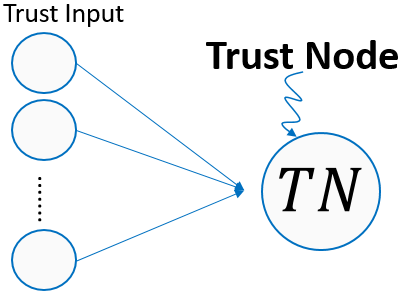
\includegraphics[width=\textwidth]{good_figs/trust_node/trustnode.png}
  \caption{Trust Node}
  \label{fig:tns}
\end{subfigure}
\hfill
\begin{subfigure}{0.27\textwidth}
  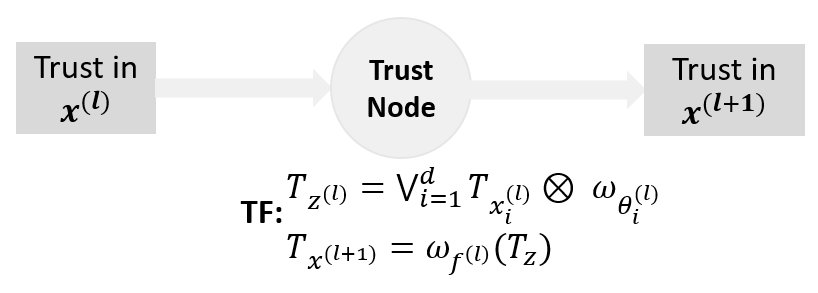
\includegraphics[width=\textwidth]{good_figs/trust_node/tnop.png}
  \caption{Trust Function operation}
  \label{fig:tnf}
\end{subfigure}
\caption{Trust Node structure and computation, mirroring the corresponding neuron (Appendix~\ref{app:trustnode}).}
\label{fig:trustnode}
\end{figure}

To extend \(\pf_\Theta\) from a single perceptron to larger networks, we introduce two fundamental concepts, the \emph{Trust Node} (\cref{fig:tns}) and the \emph{Trust Function} (\cref{fig:tnf}), which provide the basic mechanisms for propagating trust through the network structure. 

\begin{definition}[Trust Node]
A \emph{Trust Node} is an abstract computational unit associated with a neuron in a neural network. It receives trust opinions on the neuron’s inputs and produces a trust opinion on the neuron’s output. The structure of a Trust Node mirrors that of its corresponding neuron, but its computation is defined over trust opinions using operators such as discounting and fusion.
\end{definition}

\begin{definition}[Trust Function]\label{def:trustfunc}
A \emph{Trust Function} models the transformation of trust through a Trust Node. It defines how trust opinions on the inputs of a neuron are combined to produce a trust opinion on the output. 
For a neuron that computes
\(
z^{(l)} = \sum \theta^{(l)}_i \cdot x^{(l)}_i, \quad x^{(l+1)} = \phi^{(l)}(z^{(l)}),
\)
the corresponding trust computation is given by:
\begin{equation}
T_{z^{(l)}} = \bigoplus_{i=1}^{d} T_{x_{i}^{(l)}} \otimes T_{\theta_{i}^{(l)}}, \quad
T_{x^{(l+1)}} = T_{\phi^{(l)}}(T_{z^{(l)}}),
\label{eq:layerprop}
\end{equation}
where \( \otimes \) is a trust discounting operator, \(\bigoplus\) a trust fusion operator, and \( T_{\phi}^{(l)} \) the trust-equivalent of the activation function, set to the identity in this work since we use ReLU activations.
\end{definition}

As in \cref{eq:sol}, the discount operator \( \otimes \) models how trust in an input is modulated by trust in the associated parameter, while \( \bigoplus \) combines these contributions across inputs; fusion operators should be associative or generalizable~\cite{vanderheijden2018multisourcefusionoperationssubjective} to support multiple inputs. Reading the fused terms as opinions of distinct virtual sources about the same node output keeps this mapping algebraically consistent (Appendix~\ref{app:operators} gives the construction); this is precisely the consistency that variable-level fusion, as used in DeepTrust, lacks.

With these definitions in place, two challenges remain: quantifying the trustworthiness of parameters learned from datasets of variable quality, and generalizing trust propagation to deeper architectures. They motivate the Parallel Trust Assessment System (PaTAS), whose design, components, and theoretical foundations the next section presents.
\section{PaTAS For Neural Networks}\label{sec:patas}

When parameters such as \( \theta_1 \) and \( \theta_2 \) are learned by backpropagation, their trustworthiness depends on the training data: mislabeled or biased samples compromise parameter trust. The SL opinion representation of \cref{sec:backsl} further distinguishes the causes of unreliability, with distrust arising from systematic issues such as mislabeled or poisoned data and uncertainty reflecting variability or noise in the assessment. A central challenge is how to exploit this distinction in practice.

\vspace{-0.5em}
\subsection{PaTAS General Description}

To address these challenges, we introduce the \emph{Parallel Trust Assessment System (PaTAS)}, which propagates trust assessments through a neural network by operating in parallel with the standard architecture and maintaining a structure mirroring its topology. It computes trust in the output from two sources: the trust in the input features at inference time, and the trust in the parameters, derived from the trustworthiness of the training dataset (covering both the features and the labels of the training samples). To extend the perceptron principles of the previous section, PaTAS associates a Trust Node with each neuron and connects the nodes according to the network's topology, forming a Trust Nodes Network (TNN).
\begin{definition}[Trust Nodes Network]
The \emph{Trust Nodes Network} is a structured composition of Trust Nodes, one per neuron of the underlying network, mirroring its architecture; it propagates trust across layers by applying trust-specific reasoning operations aligned with the neural computation flow.
\end{definition}

PaTAS continuously evaluates trustworthiness during inference: an input \(x\) may be trustworthy (high \(T_x\)) while the output \(y\prime\) is unreliable because of biased or poorly calibrated parameters \(\theta\) (low \(T_{y\prime}\)). Embedding trust operations inside the network would alter its computations, risk harming accuracy, and raise cost; PaTAS therefore performs trust assessment in parallel (Appendix~\ref{app:flow}), so that trust reasoning never interferes with the model's predictions.




\vspace{-0.5em}
\subsection{PaTAS Design}
\begin{figure}
    \centering
    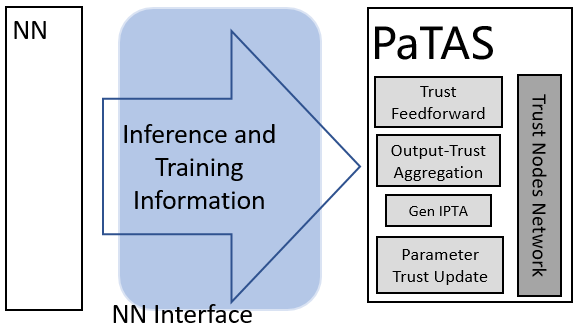
\includegraphics[width=0.43\linewidth]{good_figs/ptas/highPaTAS.png}
    \caption{High-Level Overview of PaTAS Integration with a Neural Network}
    \label{fig:highptas}
\end{figure}

% \subsection{PaTAS Components}\label{sec:ptasarch}



As illustrated in~\cref{fig:highptas}, PaTAS is composed of four main modules: Trust Feedforward, Output-Trust Aggregation, GenIPTA, and Parameter-Trust Update; the last parallels the role of backpropagation and receives a dedicated subsection.
\subsubsection{Trust Feedforward}

Trust Feedforward propagates trust through the Trust Node Network in alignment with the model's inference flow: at each layer, input and parameter trust are combined through the Trust Function's discounting and fusion. It produces a trust opinion per output neuron and stores the intermediate trust scores later used by the Parameter-Trust Update.

\subsubsection{Output-Trust Aggregation}

Output-Trust Aggregation combines the per-neuron output opinions into a single trust score via an SL fusion operator. Alternatively, one may read off the trust of the decided class directly: in digit classification, if the model predicts class `1', the decision trust is the opinion of that output Trust Node.

\subsubsection{Inference-Path Trust Assessment Generation(GenIPTA)}

GenIPTA dynamically constructs, for a single inference, an Inference-Path Trust Assessment (IPTA) reflecting the trustworthiness of the exact computational path taken: the activation trace recorded during that inference instantiates a temporary subnetwork containing only the Trust Nodes of the activated neurons. 

Since all neurons are typically activated to some degree while only a subset is strongly relevant, GenIPTA can also operate on truncated activation sets or weight the assessment by the activation values, so that stronger activations contribute more heavily. The functional flow of PaTAS across feedforward, backpropagation, and inference is illustrated in Appendix~\ref{app:flow}.

\vspace{-0.5em}
\subsection{Parameter-Trust Update}\label{sec:ptasfunc}
The Parameter-Trust Update adapts the trust of model parameters during training so that it reflects both the model's observed behavior and the reliability of the training data. To ground the design, recall the standard gradient-descent update for a parameter $\theta$:
\begin{equation}
\label{eq:gd1}
\theta \leftarrow \theta - l_r  \frac{\partial \mathcal{L}}{\partial \theta},
\end{equation}
where $l_r$ is the learning rate, $\mathcal{L}$ is the loss function, and $\frac{\partial \mathcal{L}}{\partial \theta}$ is the gradient. These gradients are computed recursively using the chain rule:
\begin{equation}
\label{eq:gd2}
\frac{\partial \mathcal{L}}{\partial \theta^{(l)}_{i,j}}
= \delta^{(l)}_i x^{(l-1)}_j,
\end{equation}
where $\theta^{(l)}_{i,j}$ denotes the weight connecting neuron $j$ in layer $(l-1)$ to neuron $i$ in layer $l$, $\delta^{(l)}_i$ is the error term of neuron $i$, and $x^{(l-1)}_j$ is the activation from the previous layer.

\Cref{eq:gd2} shows that gradients factor into an error term and an input activation, so parameter updates depend jointly on gradient signals, input activations, and learning dynamics; PaTAS mirrors this by using gradient information, input feature trust, and label trust as evidence in the Parameter-Trust Update. Notation is summarized in Appendix~\ref{app:symbols}; the complete procedure is \cref{alg:trustupdate}.

\begin{algorithm}
\caption{Parameter-Trust Update: revises each parameter's trust from gradient evidence, label trust, and neuron input trust under mini-batch training (helper functions in Appendix~\ref{app:algorithm}).}
\begin{algorithmic}[1]
    \Function{ParameterTrustUpdate}{$g, T_y, \epsilon$}
        \State $T_{y_\text{batch}}  \longleftarrow  \bigwedge_{y \in y_\text{batch}} T_y$ \Comment{aggregate label trust}
        \For{each layer $l$}
            \For{each neuron $n_i^{(l)}$}
                \State $g^{(l)}_i  \longleftarrow  \{\, g^{(l)}_{i,j} \;|\; j \in \mathcal{N}(i)\,\}$
                \State $T_{n_i \mid y_\text{batch}}  \longleftarrow $ \Call{NodeTrust}{$g^{(l)}_i, T_{y_\text{batch}}, \epsilon$}
                \State $T_{n_i \parallel Y_\text{batch}}  \longleftarrow $ \Call{DeduceTrust}{$T_{n_i \mid y_\text{batch}}, T_{n_i \mid \overline{y_\text{batch}}}, T_{y_\text{batch}}$}
                \For{each incoming edge $j$ to $n_i^{(l)}$}
                    \State $T_{\theta_{i,j}^{(l)}}  \longleftarrow $ \Call{Revise}{$T_{\theta_{i,j}^{(l)}}, T_{n_i \parallel Y_\text{batch}}$}
                    \State $T_{\theta_{i,j}^{(l)}} \longleftarrow $ \Call{Update}{$T_{\theta_{i,j}^{(l)}}, T_{x^{(l-1)}_j}, T_{y_\text{batch}}$}
                \EndFor
            \EndFor
        \EndFor
    \EndFunction
\end{algorithmic}
\label{alg:trustupdate}
\end{algorithm}
\Cref{alg:trustupdate} runs once per mini-batch over all layers and neurons. It first aggregates label trust, \(T_{y_\text{batch}} = \bigwedge_{y \in y_\text{batch}} T_y\), which conditions the trust in every parameter, then derives for each neuron \(n_i^{(l)}\) the opinion \( T_{n_{i}^{(l)} \mid y_\text{batch}} \) from gradient evidence, counting each incoming weight gradient with \( |g^{(l)}_{i,j}| < \epsilon\)\footnote{The threshold $\epsilon$ is not a tuned hyperparameter but a sensitivity parameter used only in \textsc{NodeTrust} to separate weak from strong gradients, selected relative to the typical gradient scale; it never affects model predictions or training dynamics.} as positive evidence \(r\) and the remainder as negative evidence \(s\), and mapping \((r,s)\) to a binomial opinion via \cref{eq:q1}. Since no evidence is available for the complementary case, \( T_{n_{i}^{(l)} \mid \overline{y_\text{batch}}} \) is vacuous, and the deduction operator \( \circledcirc \) combines the two conditionals with \( T_{y_\text{batch}} \) to give \( T_{n_{i}^{(l)} \parallel Y_\text{batch}} \).

For each incoming edge \(j\), the parameter trust is then revised with the deduced neuron trust, \(T_{\theta_{i,j}^{(l)}} \leftarrow T_{\theta_{i,j}^{(l)}} \circleddash T_{n_{i}^{(l)} \parallel Y_\text{batch}}\), and adjusted for the auxiliary factors that also drive the gradient update in \cref{eq:gd1,eq:gd2}, namely the learning rate, the input feature, and the batch labels:
\begin{equation}
    T_{\theta_{i,j}^{(l)}} \longleftarrow T_{\theta_{i,j}^{(l)}} \odot (T_{x_j^{(l-1)}} \oslash T_{y_\text{batch}}),
\end{equation}
where $\odot$ is binomial multiplication and $\oslash$ is the conservative combination \((b,d,u)\) with \(b = \min(b_1,b_2)\), \(d = \max(d_1,d_2)\), \(u = 1-(b+d)\). This reflects that both unreliable features and mislabeled data can strongly bias parameter updates: trust cannot exceed the weakest evidence and distrust must reflect the strongest warning. Bias terms receive the same treatment: each bias is handled as one additional parameter row whose input carries a vacuous opinion during propagation and whose trust opinion is revised exactly like any weight.

This process refines the trust in each parameter by incorporating both gradient-based behavioral evidence and auxiliary trust factors, allowing the PaTAS to align parameter trust with the training dynamics of the neural network. 

The mapping from gradient magnitude to evidence deserves explicit justification, since a large gradient does not, in isolation, imply an untrustworthy parameter. Two points make the interpretation well founded in PaTAS. First, evidence is \emph{relative}: gradients are not thresholded against an absolute constant but against the prevailing gradient scale through $\epsilon$, so the update reacts to a parameter that keeps receiving atypically large corrections \emph{after} the model has otherwise settled, not to the large gradients that are normal early in training. Second, evidence is \emph{conditional on label trust}: the same large gradient leads to a negative update of the trust assigned to the parameters only insofar as it is driven by data the model trusts. Under trusted labels, a parameter that the network must repeatedly and strongly correct is one whose learned value the trusted data does not support, which is precisely the signal PaTAS accumulates as reduced trust. Under distrusted or uncertain labels, the deduction through $T_{y_\text{batch}}$ discounts that same signal proportionally; the asymptotic cases are summarized in Appendix~\ref{app:asymptotic}. Gradient magnitude is nonetheless a proxy and can be confounded by learning-rate schedules, mini-batch noise, or saddle-point regions; a more direct evidence model for parameter reliability, together with an ablation over $\epsilon$ and gradient statistics, is left to future work.

\paragraph*{Computational Overhead}
PaTAS mirrors the network's computational flow over four-component opinions rather than scalars, so \(T_{\text{PaTAS}} \approx 3\,T_{\text{NN}}\) and \(T_{\text{with PaTAS}} \approx T_{\text{comm}} + 3\,T_{\text{NN}}\), with \(T_{\text{comm}}\) the communication overhead. Because training requires no value from PaTAS, the neural network can proceed while trust assessment completes.

\vspace{-0.5em}
\subsection{Theoretical Properties of PaTAS}\label{sec:ptastheory}
We first establish fundamental properties describing the stability and consistency of PaTAS.
\subsubsection{Convergence of PaTAS}
% \todo[inline]{Discuss convergence of PaTAS in case of convergence of input}
\label{sec:ptas_convergence}

During training, PaTAS revises the trust opinions on network parameters from trust opinions on the inputs, labels, hyperparameters, and gradient information, as outlined in \cref{alg:trustupdate}. Theorem~\ref{thm:convergence} establishes that this recursive update converges under an explicitly stated idealization of stable training; the training-time behavior under mini-batch noise is assessed empirically.

% Before delving into the specifics of PaTAS convergence, we first present a key theorem that will serve as a foundational tool in establishing the convergence properties of PaTAS.


\begin{theorem}[Convergence of PaTAS Creation]\label{thm:convergence}
\footnote{All proofs of the theorems in this section, as well as additional theoretical results, are provided in Appendix~\ref{app:proof}.}

Assume (i) the parameter opinions are initialized non-dogmatically (PaTAS initializes them as vacuous), and (ii) the per-batch revision opinion applied to each parameter stabilizes to a fixed opinion $q$: an idealization of a network trained to convergence with stationary gradient statistics and stable $T_x$, $T_y$, and $\epsilon$.
Let $T_\theta^{(n)}$ denote the trust opinion at iteration $n$ for parameter $\theta$. If the revision is performed as specified in \cref{alg:trustupdate}, then $T_\theta^{(n)}$ converges; for averaging-fusion revision the limit is $q$, at the geometric rate of Theorem~\ref{thm:arithm}.
\end{theorem}
Under actual mini-batch training the revision opinion fluctuates from batch to batch, so the theorem guarantees the consistency of the revision dynamics rather than convergence of the stochastic process itself; empirically, after accuracy convergence the trust trajectories oscillate within a narrow band around a stable level (Appendix~\ref{app:expres}).
\subsubsection{Symmetry and Invariance Properties of PaTAS}\label{sec:ptassyminv}

\begin{theorem}[Consistency Properties of PaTAS]\label{thm:infvac}
Let \(\omega^\emptyset=(0,0,1,a)\) be a vacuous binomial opinion and let \(\bar{x}=(d,b,u,a)\) denote the symmetric counterpart of \(x=(b,d,u,a)\). Then, for any parameter trust configuration \(T_\theta\):
\begin{enumerate}
    \item \emph{Vacuity is preserved.} Discounting a vacuous opinion is vacuous, \(\omega^A_B \otimes \omega^\emptyset = \omega^\emptyset\), and hence \(\mathrm{IPTA}(\omega^\emptyset) = \omega^\emptyset\).
    \item \emph{Inference is symmetric.} The outputs \(y = T_\theta(x)\) and \(\bar y = T_\theta(\bar x)\) satisfy \(u_y = u_{\bar y}\), \(b_y = d_{\bar y}\), and \(d_y = b_{\bar y}\). In particular a fully trusted input \((1,0,0)\) yields \(d_y = 0\), and a fully distrusted input \((0,1,0)\) yields \(b_{\bar y} = 0\).
\end{enumerate}
\end{theorem}

These properties are consistency guarantees rather than the paper's headline result: they establish that the trust computation is well behaved and justify reasoning about only the trusted-input case in the evaluation. Stronger, security-specific guarantees, such as provable bounds on trust degradation under a bounded poisoning adversary, are not claimed here and are left to future work.


\vspace{-0.5em}
\section{Evaluation and Results}\label{sec:evaluation}

Our evaluation shows that PaTAS produces trust estimates that converge during training, respect the properties of \cref{sec:ptastheory}, and remain interpretable under noisy features, corrupted labels, and adversarial perturbations.

We conduct four experiments of increasing complexity: (1)~\emph{Breast Cancer Classification} on a small tabular medical dataset; (2)~\emph{MNIST Digit Classification} across architectures under controlled uncertainty; (3)~\emph{Poisoned MNIST} under adversarial corruption; and (4)~\emph{Comparative Trust Evaluation} against established uncertainty baselines on out-of-distribution and corruption detection, characterizing when input-level trust is informative.

\vspace{-0.5em}
\subsection{Experimental Setup }
\subsubsection{Experiment 1 - Breast Cancer Classification}\label{exp:1}
We use the \href{https://archive.ics.uci.edu/dataset/17/breast+cancer+wisconsin+diagnostic}{Breast Cancer Wisconsin (Diagnostic) Dataset}~\cite{breastcancer-wisconsin}, 569 samples with 30 numeric features (e.g., radius, area, symmetry) derived from breast mass fine needle aspirates, classified into benign or malignant. The network has 30 input, 16 hidden (ReLU), and 2 output (Softmax) neurons, trained for 15 epochs with batch size 64 and learning rate 0.2, reaching 97\% test accuracy on unmodified data.

We degrade the training data in controlled ways and assign corresponding trust assessments, combining three extreme profiles for features and labels alike, fully trusted \((1,0,0)\), fully distrusted \((0,1,0)\), and fully uncertain \((0,0,1)\), into nine cases; these dogmatic and vacuous opinions are the canonical SL boundary cases.

Degradation is simulated with controlled perturbation functions (Appendix~\ref{app:perturb}): uncertain features receive additive uniform noise clipped to the valid range, distrusted features are resampled uniformly, and labels are degraded analogously through random noise (uncertainty) or complete replacement (distrust).

Finally, two intermediate scenarios complement the boundary cases (last two rows of \cref{tab:cancer_results}): the fully uncertain features-and-labels setting re-assessed as the mixed opinion \((0.25,0.25,0.5)\), and a mild degradation where features are perturbed with probability 0.15 and assessed as \((0.25,0,0.75)\).

\subsubsection{Experiment 2 - MNIST}\label{exp:2}

We evaluate PaTAS on MNIST~\cite{lecun1998mnist} (60{,}000 training and 10{,}000 test \(28\times28\) images, ten classes) with four architectures of increasing width, 784-16-10 through 784-128-10; not state of the art, but sufficient to expose how trust propagates across model sizes. Each uses ReLU and Softmax, trained for 20 epochs with batch size 128 and learning rate 0.05, reaching 99\% test accuracy on fully trusted data; the gradient-evidence threshold is $\epsilon = 0.05$ here and in Experiments 3 and 4. Feature and label trust assessments are fully uncertain, corresponding to no knowledge of the dataset; for contrast we repeat the smallest architecture with a fully trusted assessment.

\subsubsection{Experiment 3 - Poisoned MNIST}\label{exp:3}
We poison one third of the MNIST training images by flipping the labels of digits 6 and 9 while adding a visible fixed-size patch at the top-left corner, following common backdoor practice~\cite{chen2017targetedbackdoorattacksdeep}; the remaining two thirds stay clean. Using the 784-128-10 architecture, patch pixels and the labels of patched 6s and 9s are assigned distrust and everything else trust, so PaTAS focuses on the corrupted regions while trusting the unaffected data.


\subsubsection{Experiment 4 - Comparative Trust Evaluation}\label{exp:4}
We compare the per-sample PaTAS assessment against three established uncertainty baselines: maximum softmax probability, MC~Dropout~\cite{gal2016dropoutbayesianapproximationrepresenting} ($T{=}30$ passes, $p{=}0.2$), and Evidential Deep Learning~\cite{sensoy2018evidentialdeeplearningquantify}, each trained with the modifications its method requires under the shared architecture, optimizer, and epoch budget; DeepTrust~\cite{10.3389/frai.2020.00054} has no public implementation and is discussed in \cref{sec:rw}. Primary datasets are MNIST and Fashion-MNIST~\cite{xiao2017fashionmnist} (784-512-10, 20 epochs); GTSRB~\cite{GTSRB} (1024-128-43, features standardized with train statistics) serves as an applicability-boundary case discussed below.

The PaTAS assessment instantiates route~(ii), estimation from data, of \cref{sec:acquisition}: each input feature receives a trust opinion from its conformity to the training-data statistics, mapped through the same Baseline-Prior Quantification as parameter trust (\cref{eq:q1}), with per-feature evidence weighted by the feature's reliability as a witness, $w_j = (\sigma_{\mathrm{ref}}/\sigma_j)^2$ (full construction and parameters in Appendix~\ref{app:conformity}). The trust factor is the serial discount $P = P_{\mathrm{model}} \cdot P_{\mathrm{input}}$ of the IPTA path trust under a fully trusted input and the pooled input conformity, and the reported score anchors the discounted confidence at the class prior, $P \cdot \hat{p} + (1-P)/K$. Every method is evaluated identically on clean test data, under Bernoulli-uniform feature corruption ($p \in \{0.3, 0.6\}$, amplitude scaled to the feature range), on a mixed batch pooling clean and corrupted inputs 1:1, and as an OOD detector (the OOD set passes through the identical preprocessing: Fashion-MNIST for MNIST and vice versa); post-hoc isotonic calibration is fit per method on a held-out clean split. Results are mean~$\pm$~std over three evaluation seeds.

\paragraph*{Implementation Details for All Experiments}
Feedforward multiplications are implemented as SL trust discounting and additions as generalized SL averaging fusion (\cref{def:trustfunc}; operational flow in \cref{fig:ptasoperation}); trust revision uses the same fusion. The full Python/NumPy implementation and all experiment scripts are available as \suppp, with instructions for reproducing every experiment.

\vspace{-0.5em}
\subsection{Results and Analysis}
Evaluation is performed during training: after each feedforward/backpropagation iteration we assess the output trustworthiness under three boundary input profiles, fully trusted, fully uncertain, and fully distrusted, tracking the trust, uncertainty, and distrust mass over training, i.e., nine curves per experiment (Experiments 1--3)\footnote{The base rate is set to $0.5$, the maximum-entropy choice over $\{\text{trust}, \text{distrust}\}$, and held constant across all experiments; the score anchoring in \cref{exp:4} uses the class prior $1/K$ where a prior probability of correctness is the natural reference. A systematic sensitivity study of the base rate is left to future work.}. Results are collected in Appendix~\ref{app:expres} and summarized in \cref{tab:cancer_results,tab:mnist,tab:mnistpois,tab:mnistpoisipta}; they confirm several properties proven in \cref{sec:ptastheory}: \emph{stability} (after accuracy converges, the trust assessment settles into a narrow band, the empirical counterpart of the idealized convergence in \cref{thm:convergence}), \emph{vacuity preservation} (a fully uncertain input always produces a fully uncertain output), and \emph{symmetry} (symmetric input trust assessments yield symmetric inference results).

\begin{table*}[ht]
\begin{minipage}{0.63\textwidth}
\centering\footnotesize
\begin{tabular}{cccccc}
\hline
X Trust Assessment & Y Trust Assessment& \(\epsilon = 0.01\) & \(\epsilon = 0.1\) & Train (\%) & Test (\%) \\
\hline
fully distrusted & any & 0 & 0 & 47--58 & 41--55 \\
any & fully distrusted & 0 & 0 & 96--98 & 3--4 \\
fully uncertain & fully uncertain & 0.17 & 0.28 & 66 & 85 \\ % noise-noise
% \hline
fully uncertain & fully trusted & 0.15 & 0.32 & 96 & 96 \\ % noise-clean
% \hline
 fully trusted & fully uncertain & 0.12 & 0.29 & 69 & 94 \\ % clean-noise
% \hline
fully trusted & fully trusted & 0.62 & 0.88 & 98 & 97 \\ % clean-clean
(0.25, 0.25, 0.5) & (0.25, 0.25, 0.5)& 0.06 & 0.11 & 66 & 85 \\
% \hline
(0.25, 0, 0.75) & (0.25, 0, 0.75)& 0.20 & 0.35 & 75 & 94\\
% \hline

\hline
\end{tabular}
\caption{Breast Cancer: final trust mass and train/test accuracy (\%). Rows with a fully distrusted assessment collapse to zero trust and are grouped: distrusted features give train 47--58\% and test 41--55\%, distrusted labels give train 96--98\% and test 3--4\%.}
\label{tab:cancer_results}
\end{minipage}
\hfill
\begin{minipage}{0.37\textwidth}
\centering\footnotesize
\begin{tabular}{cccc}
\hline
Hidden Neurons & Trust \(t\) & Train (\%) & Test (\%) \\
\hline
16 & 0.306 & 65 & 72\\
% \hline
32 & 0.325 & 66 & 89 \\
% \hline
64 & 0.333 & 67 & 90\\
% \hline
128 & 0.337 & 68 & 93\\
% \hline
16 (trust) & 0.778 & 96 & 95\\
\hline
\end{tabular}
\caption{MNIST: final trust mass per architecture.}
\label{tab:mnist}
\end{minipage}

\end{table*}


We therefore report only the fully trusted input case in detail: uncertain inputs yield uncertain outputs, symmetry makes the distrusted case a mirror of the trusted one (\cref{thm:infvac}), and under trusted inputs the distrust mass stays near zero, so the trust mass alone determines the opinion; the tables report its converged value.


\subsubsection*{Experiment 1 -- Breast Cancer Classification}
Corrupted labels mislead rather than prevent learning: training accuracy stays high (96--98\%) while test accuracy collapses to near zero; corrupted features eliminate learning in every setting (41--55\% test, near chance), while label noise depresses training accuracy (69\%) yet still permits generalization (94\%).

We evaluated the system for two values of $\epsilon$ (0.1 and 0.01), the threshold used by the NodeTrust function in \cref{alg:trustupdate}, as summarized in \cref{tab:cancer_results}. For $\epsilon = 0.1$, trust mass under an uncertain $X$ stabilizes around 0.28 for uncertain $Y$ and 0.32 for trusted $Y$; a fully trusted $X$ gives 0.29 for uncertain $Y$ and $0.88$ for trusted $Y$, and whatever the $\epsilon$ value, a distrusted $X$ or $Y$ drives the trust mass rapidly to 0. For $\epsilon = 0.01$ the system reads more gradients as large and all partial-trust configurations drop (0.12--0.17); notably, under degraded features the trusted-$Y$ case falls \emph{below} the uncertain-$Y$ case (0.15 vs.\ 0.17), since trusted labels turn persistent gradient corrections into negative evidence, the mechanism analyzed in \cref{sec:acquisition}.
Overall, trust mass correlates strongly with test accuracy among the non-distrusted configurations. Two findings stand out. First, \emph{label trust matters more than feature trust}: fully uncertain $X$ with trusted $Y$ yields a higher trust mass (0.32) than trusted $X$ with uncertain $Y$ (0.29). Second, \emph{distrust is more damaging than uncertainty}: replacing the fully uncertain opinion $(0,0,1)$ on both $X$ and $Y$ with the mixed assessment $(0.25,0.25,0.5)$ reduces the trust mass from $0.28$ to $0.11$.




\subsubsection*{Experiment 2 -- MNIST Dataset}
PaTAS produces ten output trust opinions, one per class; as they are almost identical we record only the aggregated trust mass. As shown in \cref{tab:mnist}, under noisy features and labels accuracy improves with model size, and test accuracy consistently exceeds training accuracy, suggesting training noise makes the model underestimate its learning progress. Trust also increases with model size, but with diminishing gains (0.306 $\to$ 0.325 $\to$ 0.333 $\to$ 0.337), contrasting sharply with the fully trusted evaluation on the smallest architecture (0.778): \emph{training a smaller architecture on trusted data benefits trust far more than training a larger architecture on uncertain data}. Larger architectures also yield more stable assessments, likely due to smaller average gradient magnitudes.


\subsubsection*{Experiment 3 – Poisoned MNIST Dataset}
PaTAS again produces ten output trust opinions, now informative because the reliability of the inference path varies across labels when some are patched and others are not. \Cref{tab:mnistpois} reports the trust mass for label 3 (clean) and label 6 (poisoned; see \cref{exp:3}), together with clean and patched test accuracy for both digits.

Across all patch sizes the trust mass of label 3 remains higher than that of label 6 by a wide margin (e.g., 0.90 vs.\ 0.58 for the $4\times4$ patch), confirming that PaTAS reliably distinguishes clean from poisoned inference paths. Both values decrease as the patch grows, since larger patches affect more neurons along the inference path, reducing the reliability of the associated parameters and progressively touching even the neurons of clean classes; degradation is largest at $27 \times 27$, where the patch dominates nearly the entire input (0.70 and 0.49), while the clean--poisoned separation remains interpretable at every size.

To evaluate the IPTA, \cref{tab:mnistpoisipta} reports accuracy and trust opinions obtained by feedforwarding a fully trusted opinion through the IPTA derived from clean digit-3, clean digit-6, and patched digit-6 images. The backdoor is near-total in this run (patched 6s are misclassified in 99\% of cases), and the assessment exposes it sharply: clean digit-6 samples retain high accuracy (97.4\%) yet carry a markedly lower trust mass ($0.570$) than clean digit-3 samples ($0.886$), because the parameters along the digit-6 inference path were learned from poisoned data: an accurate prediction whose supporting evidence PaTAS refuses to endorse, precisely the reliability gap that confidence scores do not reveal. Patched samples inherit the same reduced trust and elevated uncertainty ($0.571$, $u = 0.429$), and explicitly distrusting the patch pixels additionally surfaces a non-zero distrust mass ($0.560, 0.011, 0.429$). PaTAS thus provides interpretable warnings about poisoned outputs even when accuracy alone looks healthy.

\begin{table}[ht]
\centering\footnotesize
\setlength{\tabcolsep}{4pt}
\begin{tabular}{ccccccc}
\hline
Patch & \multicolumn{2}{c}{Trust} & \multicolumn{2}{c}{Clean acc.\ (\%)} & \multicolumn{2}{c}{Patched acc.\ (\%)} \\
size & 3 & 6 & 3 & 6 & 3 & 6 \\
\hline
\((1 \times 1)\) & 0.897 & 0.577 & 97.92 & 97.29 & 78.22 & 0.84 \\
\((4 \times 4)\) & 0.895 & 0.576 & 97.82 & 97.39 & 39.60 & 1.04 \\
\((10 \times 10)\) & 0.881 & 0.570 & 97.92 & 97.39 & 22.08 & 0.84 \\
\((27 \times 27)\) & 0.697 & 0.490 & 97.92 & 97.29 & 0 & 0 \\
\hline
\end{tabular}
\caption{Poisoned MNIST; overall train/test accuracy (96.4--99.6\%/97.7--97.8\% across patch sizes) is omitted.}
\label{tab:mnistpois}
\end{table}

\begin{table}[ht]
\centering\footnotesize
\begin{tabular}{ccccccccc}
\hline
 & Accuracy (\%) & Trust  & Distrust & Uncertainty \\
\hline
Clean 3 & 97.82 & 0.886 & 0.0 & 0.114\\

Clean 6  & 97.39 & 0.570 & 0.0 & 0.430\\

6 with patch& 1.04 & 0.571 & 0.0 & 0.429\\

6 with patch & -- & 0.560 & 0.011 & 0.429\\
(patch distrusted) &&&&\\
\hline
\end{tabular}
\caption{IPTA on the poisoned model ($4\times 4$ patch, single run; the backdoor drives patched-6 accuracy to 1\%), feedforwarding a fully trusted opinion; in the last row patch pixels are explicitly distrusted. The poisoned class carries reduced trust even on clean, correctly classified inputs.}
\label{tab:mnistpoisipta}
\end{table}

\subsubsection*{Experiment 4 -- Comparative Trust Evaluation}
\Cref{tab:comparative} reports the two detection tasks in which trust and confidence should differ: recognizing out-of-distribution inputs, and recognizing corrupted inputs inside a mixed batch. PaTAS separates MNIST from Fashion-MNIST at $0.975$ AUROC (FPR@95 $0.145$), against $0.883/0.413$ for softmax and $0.936/0.310$ for MC~Dropout, and detects corrupted inputs at $0.972$ (MNIST) and $0.835$ (Fashion-MNIST) where every confidence-based baseline remains near chance ($0.51$--$0.63$). The ablation row attributes the mechanism: replacing the conformity-based input opinions with the constant fully-trusted opinion collapses PaTAS to baseline level ($0.896/0.415$ OOD, $0.639$ corruption detection), so the input-level trust of \cref{def:trustfunc}, not the confidence signal, carries the detection.

\begin{table}[ht]
\centering\footnotesize
\setlength{\tabcolsep}{3.5pt}
\begin{tabular}{lcccc}
\toprule
 & \multicolumn{2}{c}{OOD: MNIST vs.\ F-MNIST} & \multicolumn{2}{c}{Corruption det.\ $\uparrow$} \\
Method & AUROC $\uparrow$ & FPR@95 $\downarrow$ & MNIST & F-MNIST \\
\midrule
PaTAS (ours) & $\mathbf{0.975}{\scriptstyle\pm.001}$ & $\mathbf{0.145}$ & $\mathbf{0.972}{\scriptstyle\pm.002}$ & $\mathbf{0.835}{\scriptstyle\pm.003}$ \\
\;\;w/o input trust & $0.896$ & $0.415$ & $0.639$ & -- \\
Softmax & $0.883{\scriptstyle\pm.004}$ & $0.413$ & $0.631$ & $0.558$ \\
MC Dropout & $0.936{\scriptstyle\pm.002}$ & $0.310$ & $0.621$ & $0.545$ \\
EDL & $0.883{\scriptstyle\pm.004}$ & $0.658$ & $0.547$ & $0.510$ \\
\bottomrule
\end{tabular}
\caption{Detection of distribution violations (mean $\pm$ std, three seeds): each method's own score separates clean in-distribution inputs from OOD inputs (identical preprocessing), and clean from corrupted inputs in the mixed batch. The ablation row replaces conformity-based input opinions with the constant fully-trusted opinion.}
\label{tab:comparative}
\end{table}

On in-distribution data the two signals coincide: PaTAS matches the softmax filter on correct-vs-incorrect discrimination on clean test data ($0.979 \pm 0.003$ for both, MNIST), with equal calibration error after identical post-hoc calibration ($\mathrm{ECE}=0.006$). Under corruption they separate in the expected direction: accuracy barely drops ($97.9\% \to 97.6\%$ on the mixed batch), so the softmax retains a higher correct-vs-incorrect AUROC ($0.974$ vs.\ $0.895$) precisely because it ignores the distribution violation that PaTAS flags. Trust and confidence are thus complementary: confidence ranks correctness \emph{within} the training distribution, while trust exposes inputs that \emph{leave} it, where confident predictions are unwarranted even when correct. Directionality follows: in the reverse OOD task (Fashion-MNIST in-distribution, MNIST as OOD), MNIST digits occupy a quiet subset of Fashion-MNIST's marginals rather than violating them, and PaTAS ($0.781$) offers no advantage over MC~Dropout ($0.834$); conformity-based trust detects support \emph{violations}, not support \emph{subsets}.

\begin{table}[ht]
\centering\footnotesize
\setlength{\tabcolsep}{4.5pt}
\begin{tabular}{lccccc}
\toprule
Dataset & Med.\ $\sigma_{\mathrm{eff}}$ & $w_{\max}$ & Top-10\% & $w{\geq}4$ & Corr.\ det. \\
\midrule
MNIST & 0.47 & 52.3 & 0.32 & 0.40 & 0.972 \\
Fashion-MNIST & 0.90 & 64.0 & 0.76 & 0.18 & 0.835 \\
GTSRB & 0.98 & 1.8 & 0.14 & 0.00 & 0.545 \\
CIFAR-10 (gray) & 0.23 & 1.1 & 0.11 & 0.00 & -- \\
\bottomrule
\end{tabular}
\caption{A-priori applicability diagnostics: conformity-model statistics on each dataset's clean training features \emph{before any model is trained} (quantities defined in Appendix~\ref{app:conformity}), against the corruption detection later observed. Registered domains concentrate evidence in reliable witnesses; unregistered imagery has none, so input-level conformity is predicted, and for GTSRB confirmed, to be uninformative.}
\label{tab:diagnostics}
\end{table}

\Cref{tab:diagnostics} explains when this input-level signal exists. Fitting the conformity model on each dataset's training features yields a self-diagnostic: spatially registered domains (MNIST, Fashion-MNIST) concentrate evidence in a minority of tight-marginal ``reliable witness'' features, whose fraction even predicts the ordering of the observed detection margins ($0.40 \to 0.972$, $0.18 \to 0.835$, $0.00 \to$ chance). Unregistered imagery (GTSRB, CIFAR-10) has uniformly wide marginals, so no feature is a reliable witness and marginal conformity is predicted to be uninformative, which the full GTSRB battery confirms (corruption detection $0.545$; OOD vs.\ grayscale CIFAR-10 $0.661$ vs.\ $0.669$ for softmax). Applicability can thus be established per dataset before deployment; richer input-trust models for unregistered domains are future work.

Finally, the model-side trust provides a training-quality audit that requires \emph{no test data at all}. Training the MNIST network under increasing label-flip rates $p$ and reading the PaTAS feedforward trust under a fully trusted input (\cref{tab:audit}) shows a tripwire behavior: trust drops by $31.7\%$ relative to the clean-trained model at \emph{any} non-zero corruption rate, including $p{=}0.1$ where test accuracy moves by only $3$ points and mean confidence by $14\%$. The flat level across rates is the designed saturation of the evidence counting: already at $p{=}0.1$, a 128-sample mini-batch contains corrupted labels with probability $1-0.9^{128} \approx 1-10^{-6}$, so every batch delivers the persistent large-gradient corrections that \textsc{NodeTrust} counts as negative evidence, and the converged trust registers \emph{that} corruption is present rather than how much. Mean softmax confidence instead tracks the flip rate almost linearly and \emph{measures} severity, but reading it requires clean held-out inputs (and labels, if it is to be compared against accuracy), and a moderate value is indistinguishable from a merely difficult task. The two signals answer different questions: PaTAS detects \emph{that} training data was corrupted from the training dynamics alone; confidence quantifies the damage given labelled data.

\begin{table}[ht]
\centering\footnotesize
\setlength{\tabcolsep}{5pt}
\begin{tabular}{cccccc}
\toprule
$p$ & Test acc.\ (\%) & Mean conf. & PaTAS trust & $\Delta$trust & $\Delta$conf. \\
\midrule
0   & 97.9 & 0.981 & 0.998 & --     & --     \\
0.1 & 94.7 & 0.841 & 0.682 & 31.7\% & 14.2\% \\
0.2 & 95.7 & 0.762 & 0.682 & 31.7\% & 22.3\% \\
0.3 & 93.7 & 0.684 & 0.682 & 31.7\% & 30.3\% \\
0.4 & 91.2 & 0.589 & 0.682 & 31.7\% & 39.9\% \\
0.5 & 82.8 & 0.476 & 0.681 & 31.7\% & 51.5\% \\
\bottomrule
\end{tabular}
\caption{Training-quality audit (MNIST, 784-512-10) under label-flip rate $p$. PaTAS trust (the feedforward opinion under a fully trusted input, no test data needed) acts as a corruption tripwire ($\Delta$ = relative drop vs.\ $p{=}0$); mean softmax confidence tracks severity but requires clean held-out data.}
\label{tab:audit}
\end{table}

\vspace{-0.5em}
\section{Discussion}\label{sec:discussion}
\vspace{-0.2em}
\subsection{Discussion of PaTAS Findings}

Beyond per-output assessment, PaTAS can estimate a static trust opinion of the network as \(T(\text{NN}) = PaTAS_{FF}((1,0,0))\), on the principle that a trustworthy model preserves trust; under this definition the IPTA results of Experiment~\ref{exp:3} show clear degradation for adversarial samples (\cref{tab:mnistpoisipta}).

Although trust mass and accuracy are often correlated, our results reveal meaningful divergences. In the breast cancer task (\cref{tab:cancer_results}), the mixed profile \((0.25,0,0.75)\) yields a higher final trust mass (\(0.35\)) than the uncertain-features/trusted-label case (\(0.32\)), yet the latter achieves better test accuracy (96\% vs.\ 94\%); starkest, in poisoned MNIST (\cref{tab:mnistpoisipta}) clean digits \(3\) and \(6\) reach comparable accuracy (97.8\% and 97.4\%) but IPTA trust \(0.886\) vs.\ \(0.570\). Higher trust mass therefore does not imply superior predictive performance, and equal accuracy does not imply equal trustworthiness.

These divergences reflect that PaTAS evaluates the reliability of the inference path, not predictive accuracy alone: digit \(6\) was a poisoned class during training, so the parameters predicting it are less trusted than those for \(3\), even on clean test samples. 

Interpretation of trust values, like accuracy, is application-dependent: \((0.4,0,0.6)\) may be inadequate in high-stakes settings yet sufficient elsewhere. PaTAS supports such reading with a single interpretable metric that complements accuracy.

\paragraph*{Obtaining input and label trust}\label{sec:acquisition}
Three routes provide the input- and label-level trust opinions consumed by PaTAS, in decreasing order of information. (i) \emph{Provenance-based assessment}: when data are drawn from sources of known reliability, the quantification models of \cref{sec:back} map the supporting and contradicting evidence directly into a binomial opinion; this is how our companion work assesses dataset trustworthiness~\cite{10.1007/978-3-032-19096-3_17} and how feature-level opinions are assigned when part of an input, such as a region covered by an adversarial patch, is known to be unreliable. (ii) \emph{Estimation from data}: label agreement across annotators or models, and input-quality signals such as out-of-distribution or anomaly scores, can be converted to opinions through the same evidence mapping; the conformity-based construction of \cref{exp:4} instantiates this route. (iii) \emph{Vacuous fallback}: when no such information exists, the opinion is initialized to \((0,0,1)\); since a vacuous input yields a vacuous output (\cref{thm:infvac}), this fallback conservatively produces uncertainty-dominated assessments rather than unwarranted trust, and PaTAS still contributes through parameter and path trust. Crucially, the per-query collection circumstances of a single input are usually easier to establish than the provenance of an entire training set.

\paragraph*{Magnitude blindness, scale, and cost}
The Trust Function combines opinions independently of weight and activation magnitudes: trust deliberately tracks the provenance and reliability of the quantities entering a computation rather than their functional influence, so an input the network effectively ignores can still contribute to the output opinion. The softmax-weighted IPTA aggregation reported alongside \cref{exp:3} is a first step toward influence-aware readings, and magnitude-aware trust functions are future work. For convolutional layers, the natural extension keeps one opinion per filter weight, shared across spatial positions, with the gradient evidence of all positions fused per batch (our prototype convolutional implementation follows this design); attention layers remain open. On cost, storing one binomial opinion per parameter takes three scalars per weight, an approximately threefold memory overhead matching the analytical compute estimate; measured wall-clock overhead is reported with the revision experiments.

A key factor is the threshold \(\epsilon\) separating positive from negative gradient evidence: as \cref{tab:cancer_results} shows, too small an \(\epsilon\) makes PaTAS read gradients as large even when the model performs well, so that trusted labels reduce parameter trust, resembling the \(g \to +\infty\) case in Appendix~\ref{app:asymptotic}. \(\epsilon\) can be tuned per layer or tied to the learning rate, decaying alongside it to track the expected gradient scale. An explicit sweep over three orders of magnitude (Appendix~\ref{app:ablations}) shows a broad plateau: every reported metric is unchanged for $\epsilon \in [0.05, 1]$ and only degenerate-small values shift the operating point, so $\epsilon$ behaves as a scale parameter with a wide safe range rather than a tuned hyperparameter. The revision-fusion variant is similarly immaterial (differences at most $0.002$ across average, cumulative, and weighted fusion, Appendix~\ref{app:ablations}); averaging is retained because Theorem~\ref{thm:arithm} guarantees non-degenerate long-run behavior under repeated revision, whereas cumulative fusion drives uncertainty monotonically toward dogmatic saturation, and the independence rationale for cumulative fusion concerns feedforward fusion of feature opinions, a distinct role.

\vspace{-0.5em}
\subsection{Threat Model and Security Scope}\label{sec:threat}
\vspace{-0.5em}

\paragraph*{Assets and goal}
The asset PaTAS protects is the \emph{reliability of individual model predictions at inference time}: the defender wishes to know, per query, whether an output can be trusted given the input quality, the training-data reliability, and the parameters through which the input propagates. PaTAS is a \emph{detection and monitoring} mechanism, not a hardening one; it does not alter the model or prevent an attack, but exposes predictions with weak supporting evidence.

\paragraph*{Adversary}
We consider a \emph{training-time data-poisoning adversary}~\cite{chen2017targetedbackdoorattacksdeep} who can inject or relabel a bounded fraction of training samples, including backdoor triggers such as fixed pixel patches, to induce targeted misclassifications hidden behind high nominal accuracy and confidence. The adversary controls neither the architecture, nor the training procedure, nor the trust assessments of known-provenance data. This is the threat evaluated in \cref{exp:3}.

\paragraph*{Defender knowledge}
PaTAS assumes white-box access to the model (parameters, activations, gradients), as it runs alongside training and inference, and access to trust opinions on inputs and labels; when unavailable, these are initialized to the vacuous opinion \((0,0,1)\), yielding conservative, uncertainty-dominated assessments rather than false assurance (\cref{sec:acquisition}).

\paragraph*{Out of scope}
Evasion attacks crafted at inference time, model-stealing, and membership-inference attacks are outside the present scope; PaTAS's signals may apply to them, e.g., by monitoring the trust profile of query streams, but we make no such claim here. We likewise prove consistency properties of the trust computation (\cref{sec:ptastheory}) rather than formal robustness guarantees against a bounded adversary, which remain an open direction.


\vspace{-0.5em}
\section{Conclusion}\label{sec:conclusion}
This paper presented \emph{PaTAS}, a Subjective Logic framework propagating trust in neural networks through a parallel structure of \emph{Trust Nodes} and \emph{Trust Functions} running alongside feedforward and backpropagation; its \emph{Parameter Trust Update} and \emph{Inference-Path Trust Assessment} capture how input quality, learned parameters, and activation paths jointly shape the trustworthiness of a prediction.

Evaluation on real-world and adversarial datasets shows that PaTAS detects trust degradation caused by data poisoning and adversarial patching while remaining interpretable and stable, providing reliability information that accuracy alone does not reflect, in particular when training-data provenance is unknown. In a comparison spanning output-only uncertainty baselines and dedicated input- and feature-space detectors, the detection of distribution violations is carried by the conformity-derived input opinions, which alone outperform every dedicated detector on the violation tasks (OOD $1.000$, corruption $1.000$ on MNIST, where feature-space methods fall to $0.59$--$0.74$); trust propagation contributes what no detector expresses: a test-data-free training audit, per-class trust gaps on poisoned models that persist without oracle patch knowledge, graceful composition where a single signal fails, and in-distribution selective prediction matching the softmax filter after identical calibration. Applicability to a dataset is predictable a priori from the conformity model's own statistics (\cref{tab:diagnostics}).

Several directions remain open. The evaluation used shallow fully-connected architectures on small benchmarks; extending trust propagation to deeper convolutional and transformer models, and enriching the input-trust construction beyond marginal conformity so that unregistered imagery (GTSRB, CIFAR-10) moves inside the applicability boundary, are the primary next steps. Further studies would strengthen the framework: a sensitivity analysis under noisy or incorrect initial input and label opinions; a deeper study of the gradient-to-evidence mapping beyond the $\epsilon$ sensitivity of \cref{tab:cancer_results}; and an empirical measurement of runtime and memory overhead against the analytical $3\times$ estimate. The security scope could broaden from detection to provable robustness, with guarantees under bounded poisoning and evaluation against evasion, model-stealing, and membership-inference attacks. On the modeling side, the effect of activation functions on trust propagation is uncharacterized, and the gradient-counting used for \(T_{\theta_i \mid y_\text{batch}}\) fixes the uncertainty component by construction, motivating adaptive quantification schemes that also account for parameter magnitude.
 
% \section*{Acknowledgments}
% This should be a simple paragraph before the References to thank those individuals and institutions who have supported your work on this article.
\vspace{-1em}
\bibliographystyle{IEEEtran}
\bibliography{bibtex/bib/references, bibtex/bib/calib, bibtex/bib/ecmlbias}

\clearpage
\appendices
% \newpage
\onecolumn

\section{Subjective Logic Operators: Definitions and Examples}
\label{app:operators}
\begin{definition}[Fusion~\cite{8009820}]
\label{def:fusion-app}
Let \(A\) be an agent forming an opinion about a proposition \(X=x\) based on two information sources, \(P\) and \(Q\). The fused opinion is defined as:
\begin{equation}
    \omega^A_{X=x} = \omega^{P \& Q}_{X=x} = \omega^P_{X=x} \odot \omega^Q_{X=x}.
\end{equation}
The specific fusion operator depends on the relationship between the sources. SL defines several variants such as consensus, averaging, weighting, and cumulative fusion, each representing a distinct way of aggregating evidence. 

\textbf{Example.} Suppose two temperature sensors estimate whether the room temperature exceeds \(25^\circ\)C. If both sensors are of the same type and installed in the same place, their evidence is correlated and averaging or weighted fusion is appropriate. If they have different measurement strategies (e.g., infrared and contact-based), cumulative fusion is more suitable. The information from each independent sensor is treated as an additional, non-redundant contribution so that the combined evidence grows with each agreeing source.
\end{definition}

\begin{definition}[Trust Discounting~\cite{10706345}]
\label{def:discount}
Let \(A\) have a referral trust \(\omega^A_B\) in another agent \(B\), who holds an opinion \(\omega^B_X\) on variable \(X\). The trust-discounted opinion of \(A\) derived from \(B\)'s opinion is:
\(
    \omega^{[A;B]}_{X=x} = \omega^A_B \otimes \omega^B_{X=x} \notag
\). Referral trust is domain-specific and expresses how much \(A\) relies on \(B\) regarding \(X\).

\textbf{Example.} Consider a monitoring system where agent $A$ receives readings from a temperature sensor $B$. 
The sensor usually works well but is known to drift at times, so $A$ does not fully trust it. 
When $B$ reports that the temperature is above a safety threshold, $A$ discounts this opinion by reducing its strength and increasing uncertainty. 
This illustrates the principle of trust discounting: evidence from a partially reliable source is treated cautiously.
\end{definition}

\begin{definition}[Inferential Operators~\cite{josang2006trust}]
\label{def:inferential_ops}
Inferential operators generalize Bayesian reasoning by enabling opinion propagation through conditional relationships. 
Let \( A \) be an agent reasoning about a variable \( X \) and its potential implications for another variable \( Y \). Suppose \( A \) holds opinions \(\omega^A_{Y\mid X}\) on the relationship \(X \Rightarrow Y\).
The main operators are:
\begin{itemize}
    \item \textbf{Deduction:} derive $\omega^A_Y$ from $\omega^A_X$ using $\omega^A_{Y\mid X}$.
    \item \textbf{Abduction:} derive $\omega^A_X$ from $\omega^A_Y$ using $\omega^A_{Y\mid X}$.
\end{itemize}

\textbf{Example.} For the relation “if it rains ($X$), then Bob carries an umbrella ($Y$)”, agent $A$ holds a conditional opinion $\omega^A_{Y\mid X} = (b,d,u)$. Given an opinion on \(X\), deductive inference yields an opinion about \(Y\); conversely, abduction infers the likelihood \(X\) from \(Y\) observations.
\end{definition}



\section{Subjective Logic Operators and Notation for Parameter-Trust Update}\label{app:operator}
\begin{table}[H]
\centering
\caption{Summary of Subjective Logic Operators Used in This Work}
\label{tab:operators}
\renewcommand{\arraystretch}{1.3}
\begin{tabular}{|c|l|c|}
\hline
\textbf{Symbol} & \textbf{Name} & \textbf{Definition / Equation} \\ \hline

$\odot$ & Binomial multiplication &
\cite{josang2016subjective} \\ \hline

$\otimes$ & Trust discounting &
$\begin{aligned}
\omega^{[A;B]}_{X} &= \omega^A_B \otimes \omega^B_X \\
(b,d,u) \otimes (b',d',u') &= \left(Pb',\; Pd',\; 1-P\left(b'+d'\right)\right)\\
P &= b+au 
\end{aligned}$ \\ \hline

$\oplus$ & Fusion (averaging variant used throughout this work) &
\cite{8009820}\\ \hline

$\circleddash$ & Fusion-based revision &
$\begin{aligned}
T_{\theta} &\leftarrow T_{\theta} \circleddash T_{n \parallel Y}
\end{aligned}$ 
(as defined in Sec.~\ref{sec:ptasfunc}) \\ \hline

$\oslash$ & Conservative combination &
$\begin{aligned}
(b,d,u) &= (b_1,d_1,u_1) \oslash (b_2,d_2,u_2) \\
b &= \min(b_1,b_2), \\
d &= \max(d_1,d_2), \\
u &= 1-(b+d)
\end{aligned}$ \\ \hline

$\circledcirc $ & Deduction &
\cite{7528033,josang2016subjective}  \\ \hline

\end{tabular}
\end{table}
\begin{table}[H]
\centering
\caption{Symbols Used in the Parameter-Trust Update Subsection and Algorithm}
\label{tab:params-algorithm-append}
\renewcommand{\arraystretch}{1.2}
\begin{tabular}{ll}
\hline
\textbf{Symbol} & \textbf{Meaning / Description} \\
\hline
\multicolumn{2}{l}{\textbf{Inputs to the Algorithm}} \\
$g$ & Collection of gradients for all parameters in the batch \\
$T_y$ & Trust opinion on label $y$ \\
$\epsilon$ & Gradient sensitivity threshold in \textsc{NodeTrust} \\[4pt]

\multicolumn{2}{l}{\textbf{Batch and Layer Quantities}} \\
$T_{y_{\text{batch}}}$ & Aggregated trust over labels in the current batch \\
$l$ & Layer index \\
$n_i^{(l)}$ & Neuron $i$ in layer $l$ \\
$\mathcal{N}(i)$ & Set of incoming edges to neuron $i$ \\[4pt]

\multicolumn{2}{l}{\textbf{Gradient Evidence}} \\
$g^{(l)}_{i,j}$ & Gradient of loss w.r.t.\ $\theta^{(l)}_{i,j}$ \\
$g^{(l)}_{i}$ & Gradient vector for neuron $n_i^{(l)}$ \\
$r$ & Count of weak gradients: $|g^{(l)}_{i,j}| < \epsilon$ \\
$s$ & Count of strong gradients: $|g^{(l)}_{i,j}| \ge \epsilon$ \\[4pt]

\multicolumn{2}{l}{\textbf{Trust Values Computed in the Algorithm}} \\
$T_{n_i \mid y_{\text{batch}}}$ & Trust in neuron $n_i$ conditioned on batch labels \\
$T_{n_i \mid \overline{y_{\text{batch}}}}$ & Trust in neuron under incorrect labels (vacuous) \\
$T_{n_i \parallel Y_{\text{batch}}}$ & Deduced trust in neuron $n_i$ \\[4pt]

\multicolumn{2}{l}{\textbf{Parameter Trust}} \\
$T_{\theta^{(l)}_{i,j}}$ & Trust opinion on parameter $\theta^{(l)}_{i,j}$ \\
% $T_{lr}$ & Trust in the learning rate \\
$T_{x^{(l-1)}_j}$ & Trust in the input feature to parameter $\theta^{(l)}_{i,j}$ \\[4pt]

\multicolumn{2}{l}{\textbf{Operators Used}} \\
$\bigwedge$ & Batch-wise fusion of trust opinions \\
$\circledcirc$ & Inferential deduction operator \\
$\circleddash$ & Trust-revision operator (fusion-based revision)\\
$\odot$ & SL binomial multiplication \\
$\oslash$ & Conservative combination operator \\
\hline
\end{tabular}
\end{table}


\section{Symbols and Parameters Used in PaTAS}\label{app:symbols}
\begin{table}[H]
\centering
\caption{List of Symbols and Parameters Used in this work}
\label{tab:params-appendix}
\label{tab:params-full}
\renewcommand{\arraystretch}{1.2}
\begin{tabular}{ll}
\hline
\textbf{Symbol} & \textbf{Meaning / Description} \\
\hline
\multicolumn{2}{l}{\textbf{Neural Network Quantities}} \\
$x$ & Input feature vector \\
$y$ & Ground-truth label \\
$y' = f_\Theta(x)$ & Output of the neural network \\
$\Theta = (W,b,f)$ & Neural-network parameters (weights, biases, activations) \\
$W^{(l)}$ & Weight matrix at layer $l$ \\
$b^{(l)}$ & Bias vector at layer $l$ \\
$\phi^{(l)}(\cdot)$ & Activation function at layer $l$ \\
$z^{(l)}$ & Pre-activation vector of layer $l$ \\
$x^{(l)}$ & Activation vector of layer $l$ \\
$n_i^{(l)}$ & Neuron $i$ in layer $l$ \\
$\theta^{(l)}_{i,j}$ & Parameter from neuron $j$ in layer $l\!-\!1$ to neuron $i$ in layer $l$ \\
$\delta^{(l)}_i$ & Backpropagated error signal of neuron $i$ in layer $l$ \\
$x^{(l-1)}_j$ & Activation of neuron $j$ in the previous layer \\
$\mathcal{N}(i)$ & Set of incoming neighbors of neuron $i$ \\[4pt]

\multicolumn{2}{l}{\textbf{Gradients and Learning Dynamics}} \\
$g$ & Collection of gradients for all network parameters \\
$g^{(l)}_{i,j}$ & Gradient w.r.t.\ weight $\theta^{(l)}_{i,j}$ \\
$g^{(l)}_i$ & Vector of gradients for all incoming parameters of neuron $n_i^{(l)}$ \\
$l_r$ (or $\mathrm{lr}$) & Learning rate \\
$\mathcal{L}$ & Loss function \\[4pt]

\multicolumn{2}{l}{\textbf{Trust Assessments and Trust Nodes}} \\
$T(x)$ & Trust assessment of input features \\
$T_y$ & Trust opinion on label $y$ \\
$T_{y_{\text{batch}}}$ & Aggregated trust opinion over all labels in a batch \\
$T_{\theta^{(l)}_{i,j}}$ & Trust opinion on parameter $\theta^{(l)}_{i,j}$ \\
$T_{x^{(l)}_i}$ & Trust opinion on activation $x^{(l)}_i$ \\
$T_{x^{(l)}_j}$ & Trust opinion of feature contributing to edge $(j \to i)$ \\
% $T_{lr}$ & Trust opinion on the learning rate \\
$T_{n_i \mid y_{\text{batch}}}$ & Trust in neuron $n_i$ conditioned on batch labels \\
$T_{n_i \mid \overline{y_{\text{batch}}}}$ & Trust in neuron given incorrect labels (vacuous opinion) \\
$T_{n_i \parallel Y_{\text{batch}}}$ & Deduced trust in neuron $n_i$ after combining conditional evidence \\[4pt]

\multicolumn{2}{l}{\textbf{Subjective Logic Opinions and Evidence}} \\
$\omega = (b,d,u,a)$ & SL binomial opinion: belief, disbelief, uncertainty, base rate \\
$r$ & Positive evidence count (from weak gradients) \\
$s$ & Negative evidence count (from strong gradients) \\
$\epsilon$ & Gradient sensitivity threshold in \textsc{NodeTrust} \\[4pt]

\multicolumn{2}{l}{\textbf{Trust Operators (SL Operators + PaTAS-specific)}} \\
$\oplus$ & SL fusion operator (cumulative or averaging fusion) \\
$\otimes$ & SL trust-discounting operator \\
$\odot$ & SL binomial multiplication \\
$\oslash$ & Conservative combination operator used in parameter updates \\
$\circledcirc$ & Inferential deduction operator in PaTAS \\
$\circleddash$ & Trust-revision operator (fusion-based revision) used for parameter updates \\
$\bigwedge$ & Batch-wise fusion of trust opinions \\[4pt]

\multicolumn{2}{l}{\textbf{PaTAS System Components}} \\
$\mathrm{Pf}_\Theta$ & Parallel Trust Function (PaTAS trust feedforward) \\
\text{TNN} & Trust Nodes Network (parallel trust architecture) \\
\text{GenIPTA} & Generator of the Inference-Path Trust Assessment \\
\text{IPTA} & Inference-Path Trust Assessment for a single inference \\
\hline
\end{tabular}
\end{table}


% \section{PaTAS Operations}

% \begin{figure}[htbp]
% \centering
% \begin{subfigure}{0.48\textwidth}    
%   \includegraphics[width=\textwidth]{screen/trustagg1.png}
%   \caption{Trust Aggregation Process}
%   \label{fig:trustaggregation1}
% \end{subfigure}
% \begin{subfigure}{0.48\textwidth}
%   \includegraphics[width=\textwidth]{screen/trustagg2.png}
%   \caption{Example of Trust Aggregation Process}
%   \label{fig:trustaggregation2}
% \end{subfigure}
% \caption{Output-Trust Aggregation}
% \label{fig:trustaggregation}
% \end{figure}

% \cref{fig:trustaggregation1} illustrates this process. Each Trust Node in the output layer generates a trust score \( T_{y_1}, T_{y_2}, \ldots, T_{y_k} \), corresponding to the network’s output components. These values are then passed to an aggregation mechanism that produces a unified output trust value \( T_y \), formally defined as:
% \[
% T_y = \text{Agg} \left( (T_{y_j})_{j \in [1,k]} \right)
% \]
% where \( \text{Agg} \) is an aggregation function based on the reasoning operations defined in the PaTAS.

% \cref{fig:trustaggregation2} presents a conceptual example in which a virtual observer \( A \) receives individual trust from each output neuron. Observer \( A \) integrates these trust scores using the aggregation function to arrive at a single opinion on the network’s overall prediction trustworthiness.

% The aggregation mechanism can be adapted to different application requirements, such as majority fusion, weighted fusion, or uncertainty-sensitive operators, depending on how the output trust should reflect the underlying trust semantics.


% % \begin{figure}[htbp]
% %     \centering
% %     \includegraphics[width=0.7\linewidth]{screen/ovvwCreate.png}
% %     \caption{PaTAS Initialization and Flow Overview}
% %     \label{fig:creationdiagram}
% % \end{figure}


% % \begin{figure}
% % \centering
% % \subfloat[Overview of Neural Network]{
% %     \includegraphics[width=0.45\textwidth]{screen/nnstruct.png}
% %      \label{fig:nnstruct}
% %     }
   
% % \hfill
% % \subfloat[Overview of PaTAS]{
% %     \includegraphics[width=0.45\textwidth]{screen/ptastruct.png}
% % -   \label{fig:ptastruct}}
% % \caption{Neural Network and PaTAS}
% % \label{fig:figures}
% % \end{figure}





\section{Theorems and Proofs (\cref{sec:ptastheory})}\label{app:proof}
\subsection{Key theorems}
\begin{theorem}[Convergence of Averaging-Fusion Revision]\label{thm:arithm}
Let $\Omega = \{(b,d,u,a) \in [0,1]^4 : b+d+u = 1\}$ with the base rate $a$ held fixed, let $q = (b_q, d_q, u_q, a) \in \Omega$, and let the sequence $(\omega_n)$ be defined by the averaging-fusion revision used in our implementation,
\[
b_{n+1} = \frac{b_n u_q + b_q u_n}{u_n + u_q}, \qquad
d_{n+1} = \frac{d_n u_q + d_q u_n}{u_n + u_q}, \qquad
u_{n+1} = \frac{2\, u_n u_q}{u_n + u_q}.
\]
If $u_0 > 0$, then $\omega_n \to q$, and the convergence is geometric: with $m = \min(u_0, u_q)$,
\[
|b_{n+1} - b_q| = \lambda_n\, |b_n - b_q|, \qquad
\lambda_n = \frac{u_q}{u_n + u_q} \;\leq\; \frac{u_q}{m + u_q} < 1,
\]
and likewise for $d_n$; the uncertainty $u_n$ converges to $u_q$ monotonically, and $\lambda_n \to 1/2$. Two boundary cases complete the picture: if $u_q = 0$ and $u_0 > 0$, the sequence reaches $q$ in one step; if $u_0 = 0$, the sequence is constant, since dogmatic opinions are fixed points of averaging fusion. PaTAS avoids the latter case by initializing all parameter opinions as vacuous ($u_0 = 1$).
\end{theorem}

\begin{proof}
If $u_q = 0$ and $u_n > 0$, the update gives $b_{n+1} = b_q$, $d_{n+1} = d_q$, $u_{n+1} = 0$, so $\omega_1 = q$. If $u_0 = 0$, the update gives $b_{n+1} = b_n$, $d_{n+1} = d_n$, $u_{n+1} = 0$ for all $n$. Assume now $u_0 > 0$ and $u_q > 0$.

\emph{Uncertainty.} $u_{n+1}$ is the harmonic mean of $u_n$ and $u_q$, which lies strictly between $\min(u_n, u_q)$ and $\max(u_n, u_q)$ whenever $u_n \neq u_q$: indeed $u_{n+1} > u_q \iff 2 u_n > u_n + u_q \iff u_n > u_q$, and symmetrically for $u_n < u_q$. Hence $(u_n)$ is monotone toward $u_q$, bounded, and bounded below by $m = \min(u_0, u_q) > 0$. It converges to a limit $L \geq m$ satisfying $L = 2 L u_q/(L + u_q)$, i.e., $L (L - u_q) = 0$, hence $L = u_q$.

\emph{Belief and disbelief.} Subtracting $b_q$ from the belief update,
\[
b_{n+1} - b_q
= \frac{b_n u_q + b_q u_n - b_q (u_n + u_q)}{u_n + u_q}
= \frac{u_q}{u_n + u_q}\, (b_n - b_q),
\]
so the error contracts at every step by $\lambda_n = u_q/(u_n+u_q) \leq u_q/(m+u_q) < 1$, giving $|b_n - b_q| \leq \big(\tfrac{u_q}{m+u_q}\big)^n |b_0 - b_q| \to 0$. The same identity holds for $d_n$, the base rate is unchanged by fusion, and $u_n \to u_q$ was shown above. Hence $\omega_n \to q$, and since $u_n \to u_q$ the per-step rate satisfies $\lambda_n \to 1/2$.
\end{proof}

Averaging fusion is therefore affected by a vacuous revision opinion: for $q = (0,0,1,a)$ the theorem yields $\omega_n \to q$, i.e., repeated revision with fully uncertain evidence progressively erodes committed mass, in contrast to cumulative fusion, for which the vacuous opinion is a neutral element. No group structure on $(\Omega, \oplus)$ is required or assumed.


\begin{theorem}[Convergence of Subjective Logic Geometric Sequence]\label{thm:geo}
Let $(\Omega, \odot)$ be a group defined as in Theorem~\ref{thm:arithm}.
Let $\omega_n = (b_n, d_n, u_n, a_n) \in \Omega$ be a sequence defined recursively by the operator $\odot$ as follows:
\[
\omega_{n+1} = \omega_n \odot q,
\]
where \(q\in \Omega\) and the operator $\odot$ is the binomial multiplication defined by:
\[
\begin{cases}
b_{x \odot y} = b_x b_y + \dfrac{(1 - a_x) a_y b_x u_y + a_x (1 - a_y) u_x b_y}{1 - a_x a_y}, \\
d_{x \odot y} = d_x + d_y - d_x d_y, \\
u_{x \odot y} = u_x u_y + \dfrac{(1 - a_y) b_x u_y + (1 - a_x) u_x b_y}{1 - a_x a_y}, \\
a_{x \odot y} = a_x a_y.
\end{cases}
\]
Then the sequence $(\omega_n)$ converges in $[0,1]^4$ if $a_q < 1$. In particular:
\begin{itemize}
    \item $a_n = a_0 a_q^n \to 0$ as $n \to \infty$,
    \item $d_n \to 1$ if $d_q > 0$, and $d_n = d_0$ if $d_q = 0$,
    \item $b_n \to 0$ if $p_q = b_q + a_q u_q < 1$; if $p_q = 1$, $(b_n)$ converges to a limit within $a_0/(1-a_q)$ of $b_0$.
\end{itemize}
\end{theorem}

\begin{proof}
We analyze each component of $\omega_n$ separately.

\emph{1. Convergence of $a_n$:}  
By definition, $a_{n+1} = a_n a_q$. Since $a_q \in [0,1[$, this is a geometric sequence:
\[
a_n = a_0 a_q^n \to 0 \quad \text{as } n \to \infty.
\]

\emph{2. Convergence of $d_n$:}  
The recurrence relation is:
\[
d_{n+1} = d_n + d_q - d_n d_q = d_n (1 - d_q) + d_q.
\]
This is a first-order linear recurrence. If $d_q > 0$, the sequence is increasing and bounded above by 1. Therefore:
\[
\lim_{n \to \infty} d_n = 1\, (\text{the fixed point})
\]
If $d_q = 0$, then $d_{n+1} = d_n = d_0$ for all $n$.

\emph{3. Convergence of $b_n$:}
Separating the terms proportional to $a_n$ in the exact update gives
\[
b_{n+1} = p_q\, b_n + \delta_n, \qquad
\delta_n = \frac{a_n (1 - a_q)}{1 - a_n a_q}\,\big(u_n b_q - a_q b_n u_q\big),
\qquad p_q = b_q + a_q u_q,
\]
and since $1 - a_n a_q \geq 1 - a_q$ and $|u_n b_q - a_q b_n u_q| \leq 1$, the remainder is bounded by $|\delta_n| \leq a_n = a_0 a_q^n$, which is summable. If $p_q < 1$, unrolling the recursion yields $0 \leq b_n \leq p_q^n b_0 + \sum_{k<n} p_q^{\,n-1-k} a_0 a_q^k \to 0$, a sum of two vanishing geometric terms, so $b_n \to 0$. If $p_q = 1$, then $b_{n+1} = b_n + \delta_n$ with $\sum_k |\delta_k| \leq a_0/(1-a_q) < \infty$, so $(b_n)$ is Cauchy and converges, with limit within $a_0/(1-a_q)$ of $b_0$.

Finally, $u_n = 1 - (b_n + d_n)$ converges as the difference of convergent sequences.
\end{proof}

\subsection{Proof for Theorem~\ref{thm:convergence}}
\begin{proof}
The proof operates under the idealization stated in the theorem: the network has been trained to convergence and the batch gradients \( g \) have stabilized, so that the revision opinion applied to each parameter is fixed across iterations. Mini-batch SGD does not provide exact gradient stabilization; the empirical counterpart of this idealization, bounded oscillation of the trust trajectories after accuracy convergence, is documented in Appendix~\ref{app:expres}.

Moreover, the stability of \( T_x \), and \( T_y \)implies that trust inputs to the update mechanism are stable. Consequently, each new trust update for \( T_{\theta} \) is computed using consistent and bounded evidence, which over time results in the stabilization of the subjective opinions assigned to \( T_{\theta} \).

In detail:
\begin{itemize}
    \item \(T_x\) converging implies (\(T_{y\prime}\) converging assuming the same \(T_\theta\)) implies convergence of \(T_{y_{batch}}\).

    \item \(g\) converges so \(T_{n_i \mid y_\text{batch}}\) will remain the same. 
    
    \item since \(T_{n_i\mid \mid {Y_\text{batch}}}\) is a deterministic calculation from the convergent terms  \(T_{n_i \mid y_\text{batch}}\) and \(T_{y_{batch}}\), it follows that \(T_{n_i\mid \mid {Y_\text{batch}}}\) also converges 

    \item Finally \(T_{\theta} \longleftarrow T_{\theta} \circleddash T_{n_i\mid \mid {Y_\text{batch}}}\) converges if \(\circleddash\) is set to any fusion operator or the binomial multiplication operator (see Theorem~\ref{thm:arithm} and \ref{thm:geo} in Appendix~\ref{app:proof}). 

    \item The function \(f_{upd}\) in our implementation is based on \(T_{\theta}\), \(T_{y}\) and \({T_{x}}\) which all converge.
\end{itemize}

Therefore, assuming convergence of $T_x$, $T_y$, and $g$, the trust values for all PaTAS parameters stabilize as training progresses, proving convergence of PaTAS creation. 
\end{proof}





\subsection{Proof for \cref{thm:infvac}, Part 1 (Vacuity)}

Let \( \omega^\emptyset = (0, 0, 1, a) \) denote a vacuous binomial opinion over any variable, with arbitrary base rate \( a \in [0, 1] \). Then the following two properties hold:

\begin{enumerate}
    \item \emph{Discounting a Vacuous Opinion Yields a Vacuous Opinion.} \\
    For any trust value binomial opinion \(\omega^A_B \), the discounted opinion
    \[
    \omega^{[A;B]}_X = \omega^A_B \otimes (0,0,1,a)= (0,0,1,a)
    \]
    \textit{Proof.} Using the trust discounting operator from Subjective Logic, we set $P$ to the projected probability of \(\omega^A_B\):
    \[\omega^{[A;B]}_X = 
    \begin{cases}
    b^{[A;B]}_X = P\cdot 0 = 0, \\
    d^{[A;B]}_X = P\cdot 0 = 0, \\
    u^{[A;B]}_X = 1 - b^{[A;B]}_X-d^{[A;B]}_X = 1, \\
    a^{[A;B]}_X = a.
    \end{cases}
    \]
    Hence, \( \omega^{[A;B]} = (0,0,1,a) \).

    \item \emph{PaTAS Feedforward on Vacuous Input Yields Vacuous Output.} \\
    Let \( T_x = (0,0,1,a)\) be the trust assessment of an input to PaTAS. Then for any parameter trust configuration \( T_\theta \), the output trust assessment satisfies:
    \[
    T_y = \text{IPTA}(T_x) = (0,0,1,a).
    \]
    \textit{Proof.} The PaTAS feedforward mechanism computes for each neuron:
    \[
    T_z = \bigoplus_i \left( T_{x_i} \otimes T_{\theta_i} \right).
    \]
    Since each \( T_{x_i} = (0,0,1,a) \), and using the result from part (1), we get:
    \[
    T_{x_i} \otimes T_{\theta_i} = (0,0,1,a), \quad \forall i.
    \]
    Then, by fusion of vacuous opinions:
    \[
    T_z = \bigoplus_i (0,0,1,a) = (0,0,1,a).
    \]
    This holds recursively through all layers of PaTAS, including the output layer, hence:
    \[
    T_y = (0,0,1,a).
    \]
\end{enumerate}

\subsection{Proof for \cref{thm:infvac}, Part 2 (Symmetry)}
\begin{proof}
We prove the theorem in two steps.

\emph{(1) Symmetry of the Discount Operator:} \\
Let $\omega_\theta = (b_\theta, d_\theta, u_\theta)$ be a binomial opinion representing the trust weight associated with a connection in the PaTAS. Let $P$ denote the projected probability of $\omega_\theta$, defined as:
\[
P = b_\theta + a u_\theta,
\]
where $a$ is the base rate (typically $a = 0.5$ for binary domains).

Let $x = (b, d, u)$ be any binomial opinion and $\bar{x} = (d, b, u)$ its symmetric counterpart. Then the trust discounting operation yields:
\[
\omega_\theta \otimes x = (P \cdot b, P \cdot d, 1 - P \cdot (b + d)),
\]
\[
\omega_\theta \otimes \bar{x} = (P \cdot d, P \cdot b, 1 - P \cdot (b + d)).
\]
Since $b + d = 1 - u$, both discounted opinions have identical uncertainty and symmetric belief/disbelief masses. Hence, $\omega_\theta \otimes x$ and $\omega_\theta \otimes \bar{x}$ are symmetric.

\emph{(2) Symmetry Preservation under Fusion:} \\
Let $\mathcal{X} = \{x_1, \dots, x_n\}$ be a set of discounted opinions resulting from symmetric inputs, and let $\bar{\mathcal{X}} = \{\bar{x}_1, \dots, \bar{x}_n\}$ be their symmetric counterparts. Consider any symmetric fusion operator $\bigoplus$ (such as averaging, cumulative fusion, or consensus fusion in Subjective Logic) applied to $\mathcal{X}$ and $\bar{\mathcal{X}}$.

Since each pair $(x_i, \bar{x}_i)$ is symmetric and the operator treats belief and disbelief symmetrically, we have:
\[
\bigoplus_{i=1}^n x_i = (b', d', u') \quad \Rightarrow \quad \bigoplus_{i=1}^n \bar{x}_i = (d', b', u').
\]
Thus, the output of the PaTAS feedforward inference remains symmetric when symmetric inputs are provided.

\emph{(3) Invariance under Fusion:} \\
A fundamental property of Subjective Logic fusion operators is that if all input opinions assign the same value to a specific mass (e.g., belief or disbelief), the result will preserve that value. In particular, if all input opinions have belief mass equal to zero, the fused result will also have belief mass zero. The same applies to disbelief mass.

Therefore, if the discounting step yields discounted opinions with zero belief (or zero disbelief) across all components, then the fusion stage will preserve that zero mass in the final output.

\emph{(4) Fully Trusted and Distrusted Cases:} \\
For $x = (1, 0, 0)$ (fully trusted), we have:
\[
\omega_\theta \otimes x = (P, 0, 1 - P),
\]
so the discounted opinion assigns zero disbelief. As noted above, the fusion of such discounted opinions will also assign zero disbelief.

For $\bar{x} = (0, 1, 0)$ (fully distrusted), we have:
\[
\omega_\theta \otimes \bar{x} = (0, P, 1 - P),
\]
so the discounted opinion assigns zero belief. Therefore, the belief from a fully distrusted input is always zero in the PaTAS output.
\end{proof}


\section{Asymptotic Behavior of the Deduced Parameter Trust}
\label{app:asymptotic}

Table~\ref{tab:asymptotic} reports the asymptotic behavior 
of $T_{\theta_i \| Y_\text{batch}}$ as a function of the 
gradient magnitude $g$ and the label trust $T_{y_\text{batch}}$. 
When $g \to 0$ the neuron is assessed as Trusted regardless 
of label trust, reflecting that vanishing corrections indicate 
a well-settled parameter. When $g \to +\infty$ and labels are 
Trusted, the parameter is assessed as DisTrusted, since the 
trusted data must repeatedly and strongly correct it. Under 
Uncertain or DisTrusted labels the same large gradient produces 
a more conservative assessment, confirming that negative 
evidence is discounted in proportion to label unreliability.

\begin{table}[h]
\centering
\caption{Asymptotic behavior of $T_{\theta_i \| Y_\text{batch}}$}
\label{tab:asymptotic}
\begin{tabular}{ccc}
\toprule
$g \to$ & $T_{y_\text{batch}} \to$ & 
    $T_{\theta_i \| Y_\text{batch}} \to$ \\
\midrule
$0$ & Trusted      & Trusted      \\
    & Uncertain    & Uncertain    \\
    & DisTrusted   & Uncertain    \\
\midrule
$+\infty$ & Trusted    & DisTrusted       \\
          & Uncertain  & $(0, 0.5, 0.5)$  \\
          & DisTrusted & Uncertain        \\
\bottomrule
\end{tabular}
\end{table}




\section{Perceptron Case: Full Derivation (\cref{sec:perceptron})}\label{app:perceptron}
This appendix gives the derivation of \cref{lem:perceptron}. Throughout, we use a two-feature perceptron estimating the cost of renting an apartment,
\begin{equation}
    y\prime = 10 \times s + 100 \times n_r,
    \label{equ:smodel}
\end{equation}
where \(s\) is the size of the apartment and \(n_r\) the number of rooms, and we treat two sub-problems in turn: how trust in \(s\) and \(n_r\) propagates to \(y\prime\), and how trust in the parameters \(\theta_1 = 10\) and \(\theta_2 = 100\) refines that propagation.

\begin{figure}[H]
    \centering    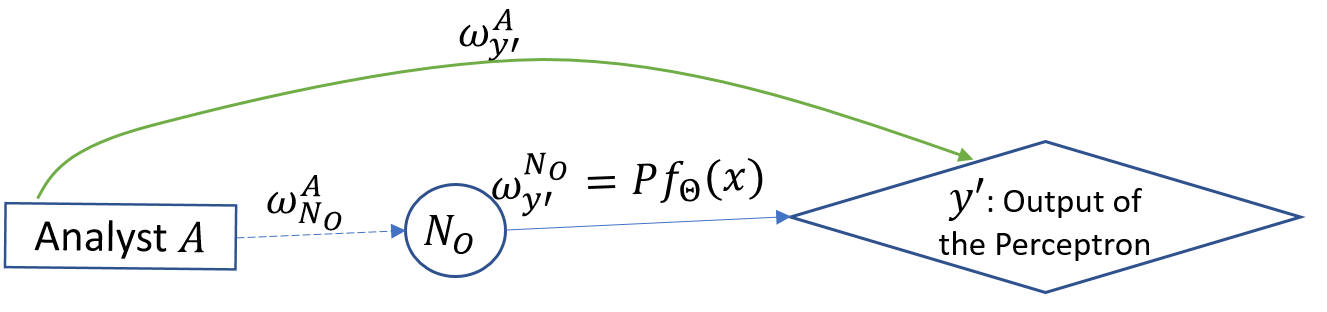
\includegraphics[scale=0.3]{img/pbstate.png}
    \caption{STN used to assess the output \(y\prime=f(x)\) of a perceptron \(\Theta\)}
    \label{fig:pbstate}
\end{figure}

% \subsection{Solution for the Perceptron}
\subsection{Trust Propagation from Input to Output}
% \todo[inline]{Describe Solution for Problem 1}
\begin{figure}
\centering
\subfloat[Perceptron for \cref{equ:smodel}]{
    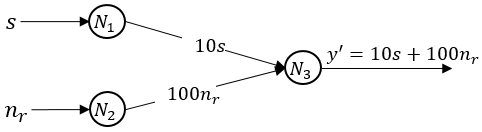
\includegraphics[width=0.35\textwidth]{img/NN1.png}
     \label{fig:nn1}
    }
   
\hfill
\subfloat[Parallel Trust Function for \cref{equ:smodel}]{
    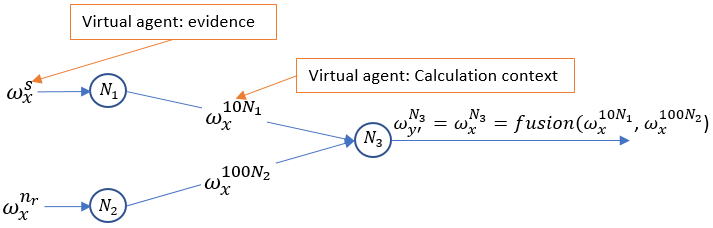
\includegraphics[width=0.45\textwidth]{img/NN1S.png}
   \label{fig:nn1s}}
\caption{Trust-propagation based solely on input-feature trust}
\label{fig:solution1}
\end{figure}
\noindent\paragraph*{Objective} Determine how trust in the individual input features (\(s\) and \(n_r\)) propagates through a simple perceptron to produce a trust assessment on the output variable \(y\prime\), representing the predicted apartment cost.
\paragraph*{Assumptions} For now, we assume that the model parameters \(\theta_1=10\) and  \(\theta_2=100\) are fully trusted and input feature trust opinions (\(T_s\) and \(T_{n_r}\)) are available.

The model specified in \cref{equ:smodel} is equivalent to the NN depicted in \cref{fig:nn1}. This network employs a linear transformation without an activation function. The input vector is:
$$ 
x = \begin{pmatrix}
    s \\
    n_r
\end{pmatrix}
$$ 
Let $\omega_x^s$ be the trust opinion on $x$ based on $s$ as evidence and  $\omega_x^{n_r}$ the trust opinion on $x$ based on $n_r$ as evidence. Since the output neuron $N_3$ computes \cref{equ:smodel}, we associate this computation with two agents: $10N_1$ from the context of computing \(10\cdot s\) and $100N_2$ from the context of computing \(100\cdot n_r\). The trust opinion of the output neuron \(N_3\) on \(x\) is then: 
\(\omega_x^{N_3} = \mathit{fusion}(\omega_x^{10N_1}, \omega_x^{100N_2})\). 

The choice of the fusion operator (that we will later denote by \(\oplus\) ) depends on the semantics of \(s\) and \(n_r\) (see Definition~\ref{def:fusion-app}). In this example, since $s$ and $n_r$ represent independent evidence, the fusion operator to use is cumulative fusion.

Assuming full trust in the parameters \(\theta_1 = 10\) and \(\theta_2 = 100\), we have:
\begin{align}
    \omega_x^{10N_1} = \omega_x^{N_1} = \omega_x^{s} = T_s \, \text{ (Trust in the feature \(s\) of \(x\))} \notag \\
    \omega_x^{100N_2} = \omega_x^{N_2} = \omega_x^{n_r} = T_{n_r} \, \text{ (Trust in the feature \(n_r\) of \(x\))} \notag 
\end{align}

Since the output value is deterministically related to the input via
\[
y' = f(x),
\]
the trust opinion of \(N_3\) on \(y'\) is the same as the trust opinion already computed for \(x\). Clearly, the transformation performed by \(f\) is encoded in the agent algebra, not in the variable algebra. Thus,
\begin{align}
    \omega_{y\prime}^{N_3} &= \omega_x^{N_3} = \omega_x^{10N_1} \oplus \omega_x^{100N_2} \notag \notag \\
&= \omega_x^{s} \oplus \omega_x^{n_r} = T_s \oplus T_{n_r}
\end{align}
In summary, if we define \(T_x = \begin{pmatrix}
    T_s&T_{n_r}
\end{pmatrix} \), then:
\[\pf_\Theta(T_x) = \pf_\Theta(\begin{pmatrix}
    T_s&T_{n_r}
\end{pmatrix}) =  T_s \oplus T_{n_r} \]


\subsection{Impact of Parameter Trust}
\paragraph*{Objective} Analyze how trust in the model parameters \(\theta_1=10\) and \(\theta_2=100\) affects the resulting trust assessment on the output \(y\prime\), given trust in the inputs.
\paragraph*{Assumption} Trust Opinions \(T_{\theta_1}\) and \(T_{\theta_2}\) are assigned to the parameters. The approach used to calculate these parameter-trust values will be discussed in Section~\ref{sec:patas}.

In problem 2, the model is expressed as:
\begin{equation}
    y\prime = \theta_1\times s + \theta_2\times n_r
    \label{equ:smodel2}
\end{equation} 
and we assume trust parameters \(T_{\theta_1}\) and \(T_{\theta_2}\) respectively in \(\theta_1\) and \(\theta_2\) (we'll see in details in Section~\ref{sec:patas} how to calculate these trust parameters). Unlike the previous problem, where we fully trusted \(\theta_1\) and \(\theta_2\), here we do not fully trust these parameters, and we must account for their trust assessments. For the network to incorporate the trust in \(\theta_1\) and \(\theta_2\), we adjust the trust opinions on the features accordingly. The trust opinions are now refined.
\begin{figure}
    \centering
    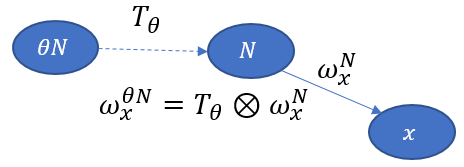
\includegraphics[width=0.4\linewidth]{img/multprob2.png}
    \caption{Trust-propagation Trust Network with parameter trust.}
    \label{fig:multprob2l}
\end{figure}
As depicted in \cref{fig:multprob2l}, we model this as a small subjective network. therefore:
\begin{align}
    \omega_x^{\theta_1 N_1} = T_{\theta_1} \otimes \omega_x^{N_1} \; \text{and} \;
    \omega_x^{\theta_1 N_2} =  T_{\theta_2} \otimes \omega_x^{N_2}
\end{align}
where \(\otimes\) is a trust discounting operator. This result is consistent with the solution for problem 1 as for fully trusted \(T_\theta=(1,0,0)\), we have \(\omega_x^{\theta N} = T_{\theta} \otimes \omega_x^{N} = \omega_x^{N}\) (for any neuron \(N\)).

Finally, the resulting output trust \(\omega_{y\prime}^{N_3}\) is calculated by the fusion of these adjusted trust opinions: 
\begin{equation}
\label{eq:sol222}
    \pf_\Theta(T_x) = \pf_\Theta(\begin{pmatrix}
    T_s&T_{n_r}
\end{pmatrix}) =  (T_{\theta_1}\otimes T_s)\oplus (T_{\theta_2}\otimes T_{n_r})
\end{equation}


Thus, we adjust the trust in the network output based on the trust in both the parameters and the features, ensuring that the trust propagation takes into account the trust in the parameters.



\section{Trust Node Structure}\label{app:trustnode}
\begin{figure}[H]
\centering
\begin{subfigure}{0.24\textwidth}
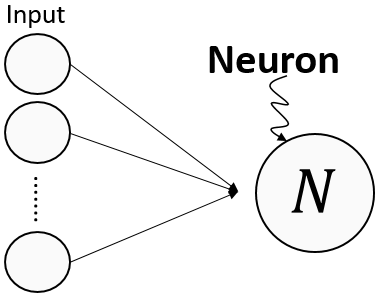
\includegraphics[width=\textwidth]{good_figs/trust_node/neuron.png}
  \caption{Structure of a Perceptron}
  \label{fig:neuron}
\end{subfigure}
\begin{subfigure}{0.24\textwidth}
  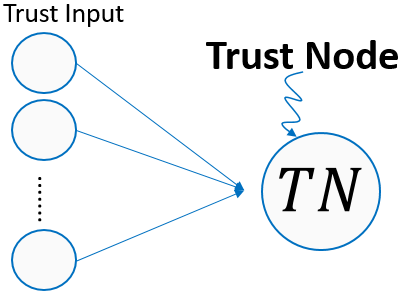
\includegraphics[width=\textwidth]{good_figs/trust_node/trustnode.png}
  \caption{Mirrored Trust Structure}
\end{subfigure}

\begin{subfigure}{0.48\textwidth}
  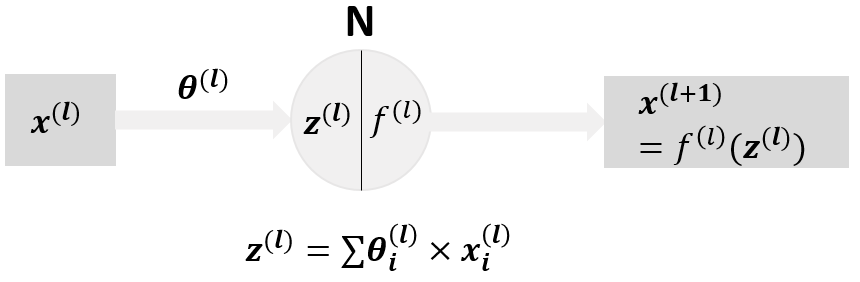
\includegraphics[width=\textwidth]{good_figs/trust_node/neurop.png}
  \caption{Perceptron Operation}
  \label{fig:neuronfunc}
\end{subfigure}
\begin{subfigure}{0.48\textwidth}
  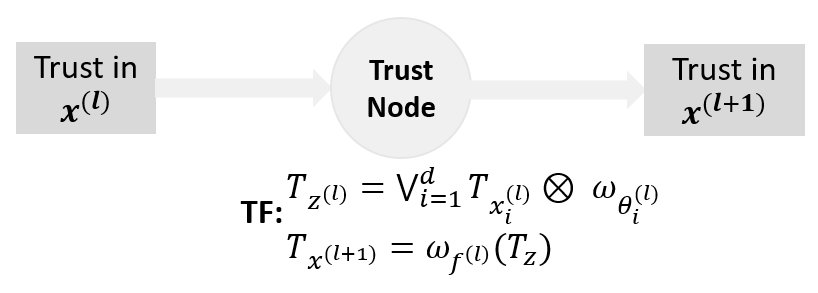
\includegraphics[width=\textwidth]{good_figs/trust_node/tnop.png}
  \caption{Trust Function Operation}
\end{subfigure}
\caption{Trust Node structure and computation, shown alongside the corresponding neuron operations.}
\label{fig:trustnodefull}
\end{figure}

\section{PaTAS Workflow and Functional Flow}\label{app:flow}
\begin{figure}[H]
    \centering
    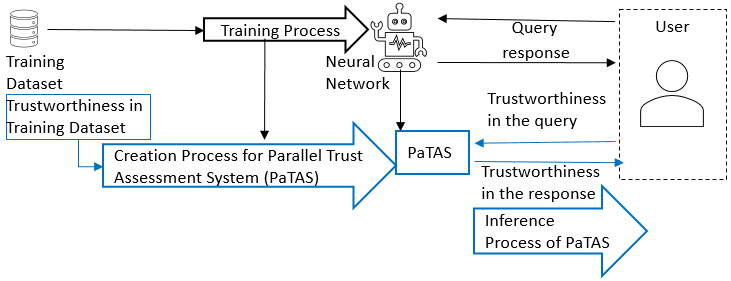
\includegraphics[width=0.75\linewidth]{screen/overviewPTAS.png}
    \caption{Overview of the PaTAS workflow.}
    \label{fig:ovvwptas}
\end{figure}

\begin{figure}[H]
    \centering
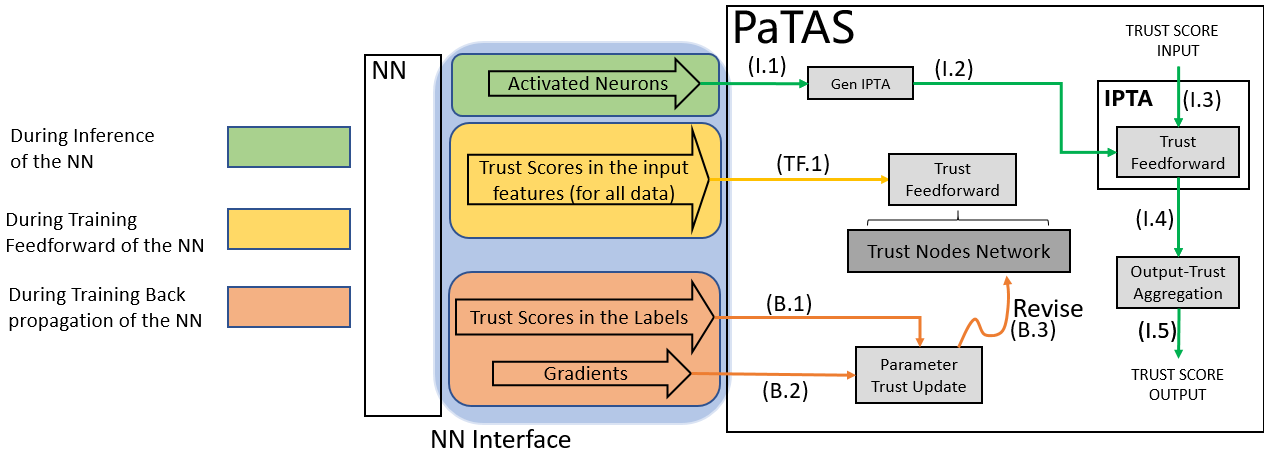
\includegraphics[width=0.85\linewidth]{good_figs/ptas/operations.png}

\caption{
    Functional flow of the PaTAS framework integrated with a neural network, illustrating how trust is propagated and revised during feedforward, backpropagation, and inference. 
    \\
    \textbf{Feedforward (Training Phase):} 
    The NN interface extracts trust scores from input features for all data being processed. These trust scores (TF.1) are passed to the \textit{Trust Feedforward} module, which propagates them through the \textit{Trust Nodes Network} in parallel with the neural computations. During training, Trust Feedforward also stores the trust scores of all intermediate computations in the NN, to be reused in backpropagation. 
    \\
    \textbf{Backpropagation (Training Phase):} 
    Once the NN computes gradients, the trust scores of the labels (B.1) and the gradients are provided to the \textit{Parameter-Trust Update}. Gradients (B.2) indicate how dataset labels affect parameter updates, while label trust determines whether these updates should be considered reliable. The stored intermediate trust values are also incorporated in this process. Finally, the \textit{Parameter-Trust Update} module refines the trust values of the Trust Nodes Network parameters (B.3), aligning them with the evolving learning dynamics. 
    \\
    \textbf{Inference Phase:} 
    During operation, contextual information such as the set of activated neurons is retrieved. This information is passed to \textit{GenIPTA} (I.1), which constructs an \textit{Inference Path Trust Assessment (IPTA)} corresponding to the specific inference path (I.2). The IPTA takes input trust scores (I.3), propagates them along the path, and produces trust scores for each NN output. These can then be passed to the \textit{Output-Trust Aggregation} (I.4) which will combine them into a single consolidated trust score representing the reliability of the prediction (I.5).
    }
    \label{fig:ptasoperation}
\end{figure}

\section{Helper Functions for \cref{alg:trustupdate}}\label{app:algorithm}
\begin{algorithm}[H]
\caption{Helper functions used by the Parameter-Trust Update}
\begin{algorithmic}[1]
    \Function{NodeTrust}{$g^{(l)}_i, T_{y_\text{batch}}, \epsilon$}
        \State Count $r$: \#edges with $|g^{(l)}_{i,j}| < \epsilon$ 
        \State Count $s$: \#edges with $|g^{(l)}_{i,j}| \geq \epsilon$ 
        \State Map $(r,s)$ into a binomial opinion using Baseline-Prior Quantification
        \State \Return $T_{n_i \mid y_\text{batch}}$
    \EndFunction

    \Function{DeduceTrust}{$T_{n_i \mid y_\text{batch}}, T_{n_i \mid \overline{y_\text{batch}}}, T_{y_\text{batch}}$}
        \State $T_{n_i \mid \overline{y_\text{batch}}}  \longleftarrow  (0,0,1)$
        \State \Return $T_{n_i \parallel Y_\text{batch}} = T_{y_\text{batch}} \circledcirc (T_{n_i \mid y_\text{batch}}, T_{n_i \mid \overline{y_\text{batch}}})$
    \EndFunction

    \Function{Revise}{$T_{\theta_{i,j}^{(l)}}, T_{n_i \parallel Y_\text{batch}}$}
        \State \Return $T_{\theta_{i,j}^{(l)}} \circleddash T_{n_i \parallel Y_\text{batch}}$
    \EndFunction
    \Function{Update}{$T_{\theta^{(l)}_{i,j}}, T_{lr}, 
    T_{x^{(l-1)}_j}, T_{y_\text{batch}}$}
    \State \Return $T_{\theta^{(l)}_{i,j}} \odot 
           (T_{x^{(l-1)}_j} \oslash T_{y_\text{batch}})$
    \EndFunction

\end{algorithmic}
\end{algorithm}

\section{Perturbation Functions Used in \cref{exp:1}}\label{app:perturb}
In practice, feature and label trust degradation may arise from poor-quality imaging, human annotation errors, or flaws in the preprocessing pipeline. 
In all experiments, we simulate degradations using controlled perturbation functions. 
For fully uncertain feature opinion, we introduce additive uniform noise 
\vspace{-1em}
\[
x' = x + \mu, \quad \mu \sim U(-\eta, \eta),
\]
where 
\(
\eta = 0.3 \times \max(\text{features}).
\)
Each feature is perturbed with probability $0.3$. 
After noise addition, if $x'$ lies outside the valid range 
$[\min(\text{features}), \max(\text{features})]$, it is clipped to the corresponding boundary:
\[
x' = 
\begin{cases}
\min(\text{features}), & x' < \min(\text{features}), \\
\max(\text{features}), & x' > \max(\text{features}), \\
x', & \text{otherwise}.
\end{cases}
\]
To model distrust, we generate corrupted inputs by sampling from a uniform distribution over the feature space:
\[
x' \sim U(\min(\text{features}), \max(\text{features})),
\]

Label degradation is modeled analogously: uncertainty is introduced via random label noise, while full distrust is represented by a complete replacement of the labels.

\section{Conformity-Based Input-Trust Construction (\cref{exp:4})}\label{app:conformity}
This appendix specifies the input-trust construction used in \cref{exp:4} precisely; all parameters are fixed once and shared by every dataset.

Let the clean training features be $x^{(1)},\dots,x^{(n)} \in \mathbb{R}^m$. For each feature $j$ we compute the marginal mean $\mu_j$ and standard deviation $\sigma_j$, and a robust span $S$ of the whole feature matrix as the difference between its $99.5$th and $0.5$th percentiles. The \emph{effective deviation} is floored at a fraction of the span,
\[
\sigma^{\mathrm{eff}}_j = \max(\sigma_j,\, 0.02\, S),
\]
so that near-constant features cannot produce unbounded standardized deviations from minimal perturbations. For an input $x$, the standardized deviation is $z_j = |x_j - \mu_j| / \sigma^{\mathrm{eff}}_j$ and the conformity is
\[
g_j = \exp\!\big(-\tfrac{1}{2}\max(z_j - 1,\, 0)^2\big) \in (0,1],
\]
so deviations within one effective standard deviation are fully conforming and only the excess erodes conformity. The \emph{reliability weight} of feature $j$ is the capped inverse-variance weight
\[
w_j = \min\!\big((\sigma_{\mathrm{ref}} / \sigma^{\mathrm{eff}}_j)^2,\, 64\big),
\qquad \sigma_{\mathrm{ref}} = \operatorname{median}_j \sigma^{\mathrm{eff}}_j,
\]
expressing that a feature with a tight training distribution is a reliable witness whose violation is unambiguous, while the cap bounds the influence any single feature can exert. Each feature contributes evidence $r_j = N w_j g_j$ and $s_j = N w_j (1-g_j)$ with base evidence mass $N = 50$, mapped to a binomial opinion by \cref{eq:q1} with $W = 2$; this is the same quantification used for parameter trust. The per-sample input trust $P_{\mathrm{input}}$ is the projected probability (base rate $0.5$) of the pooled opinion obtained by applying \cref{eq:q1} to the summed evidence $(\sum_j r_j, \sum_j s_j)$, which corresponds to cumulative fusion of independent evidence sources.

The columns of \cref{tab:diagnostics} are, in this notation: the median of $\sigma^{\mathrm{eff}}_j$, the maximum of $w_j$, the share of total weight mass held by the top decile of features ranked by $w_j$, and the fraction of features with $w_j \geq 4$. The last two are descriptive statistics of weight concentration used for reporting only (the threshold $w_j \geq 4$ corresponds to $\sigma^{\mathrm{eff}}_j$ at most half of $\sigma_{\mathrm{ref}}$); they are not parameters of the construction.

\vspace{-0.5em}
\section{Operator and Threshold Sensitivity}\label{app:ablations}
Both ablations use the MNIST 784-128-10 trust/trust scenario of \cref{exp:2} (20 epochs, 1000-sample evaluation subset, test-time feature noise $p = 0.3$ for the noisy columns).

\Cref{tab:abl-fusion} varies the trust-revision fusion operator. The converged trust mass and every downstream metric agree to within $0.002$ across averaging, cumulative, and weighted fusion, so the findings of this paper do not depend on the variant; averaging is used throughout because Theorem~\ref{thm:arithm} establishes non-degenerate long-run behavior under repeated revision, whereas cumulative fusion accumulates evidence monotonically toward dogmatic (zero-uncertainty) opinions.

\Cref{tab:abl-eps} sweeps the gradient-evidence threshold over three orders of magnitude. The trusted-input trust mass and the selective-prediction metrics are constant on the plateau $\epsilon \in [0.05, 1]$ and degrade only at degenerate-small values, where nearly every gradient is read as strong evidence; the equality of the trusted-input trust and distrusted-input distrust columns is the belief/disbelief symmetry of Theorem~\ref{thm:infvac} observed empirically.

\begin{table}[H]
\centering\footnotesize
\begin{tabular}{lccccc}
\toprule
Fusion & Trust $t_{\mathrm{tr}}$ & AUROC$_{\mathrm{cl}}$ & AUROC$_{\mathrm{no}}$ & ECE$_{\mathrm{cl}}$ & ECE$_{\mathrm{no}}$ \\
\midrule
Average (used) & 0.988 & 0.957 & 0.973 & 0.013 & 0.020 \\
Cumulative & 0.990 & 0.957 & 0.973 & 0.012 & 0.020 \\
Weighted & 0.989 & 0.957 & 0.973 & 0.013 & 0.020 \\
\bottomrule
\end{tabular}
\caption{Trust-revision fusion ablation: converged trusted-input trust mass and selective-prediction metrics on clean (cl) and feature-noised (no) test data.}
\label{tab:abl-fusion}
\end{table}

\begin{table}[H]
\centering\footnotesize
\begin{tabular}{lccccc}
\toprule
$\epsilon$ & $t_{\mathrm{tr}}$ & $d_{\mathrm{dis}}$ & AUROC$_{\mathrm{cl}}$ & AUROC$_{\mathrm{no}}$ & ECE$_{\mathrm{cl}}$ \\
\midrule
0.001 & 0.573 & 0.573 & 0.826 & 0.900 & 0.195 \\
0.01 & 0.976 & 0.976 & 0.940 & 0.964 & 0.018 \\
0.05$^{*}$ & 0.989 & 0.989 & 0.957 & 0.973 & 0.013 \\
0.1 & 0.989 & 0.989 & 0.957 & 0.973 & 0.013 \\
0.2 & 0.989 & 0.989 & 0.957 & 0.973 & 0.013 \\
0.5 & 0.989 & 0.989 & 0.957 & 0.973 & 0.013 \\
1.0 & 0.989 & 0.989 & 0.957 & 0.973 & 0.013 \\
\bottomrule
\end{tabular}
\caption{$\epsilon$ sweep ($^{*}$ = value used in Experiments 2--4): trusted-input trust $t_{\mathrm{tr}}$, distrusted-input distrust $d_{\mathrm{dis}}$ (equal by Theorem~\ref{thm:infvac}), and selective-prediction metrics. All quantities are constant on $\epsilon \in [0.05, 1]$.}
\label{tab:abl-eps}
\end{table}

\section{Detailed results}\label{app:expres}

\begin{figure}[H]
\centering
\begin{subfigure}{0.72\linewidth}
    \centering
    \includegraphics[width=\linewidth]{main_plots/plot_ptas-128-t-t-ps4.pdf}
    \caption{Trust mass}
    \label{fig:4x4}
\end{subfigure}
\begin{subfigure}{0.72\linewidth}
    \centering
    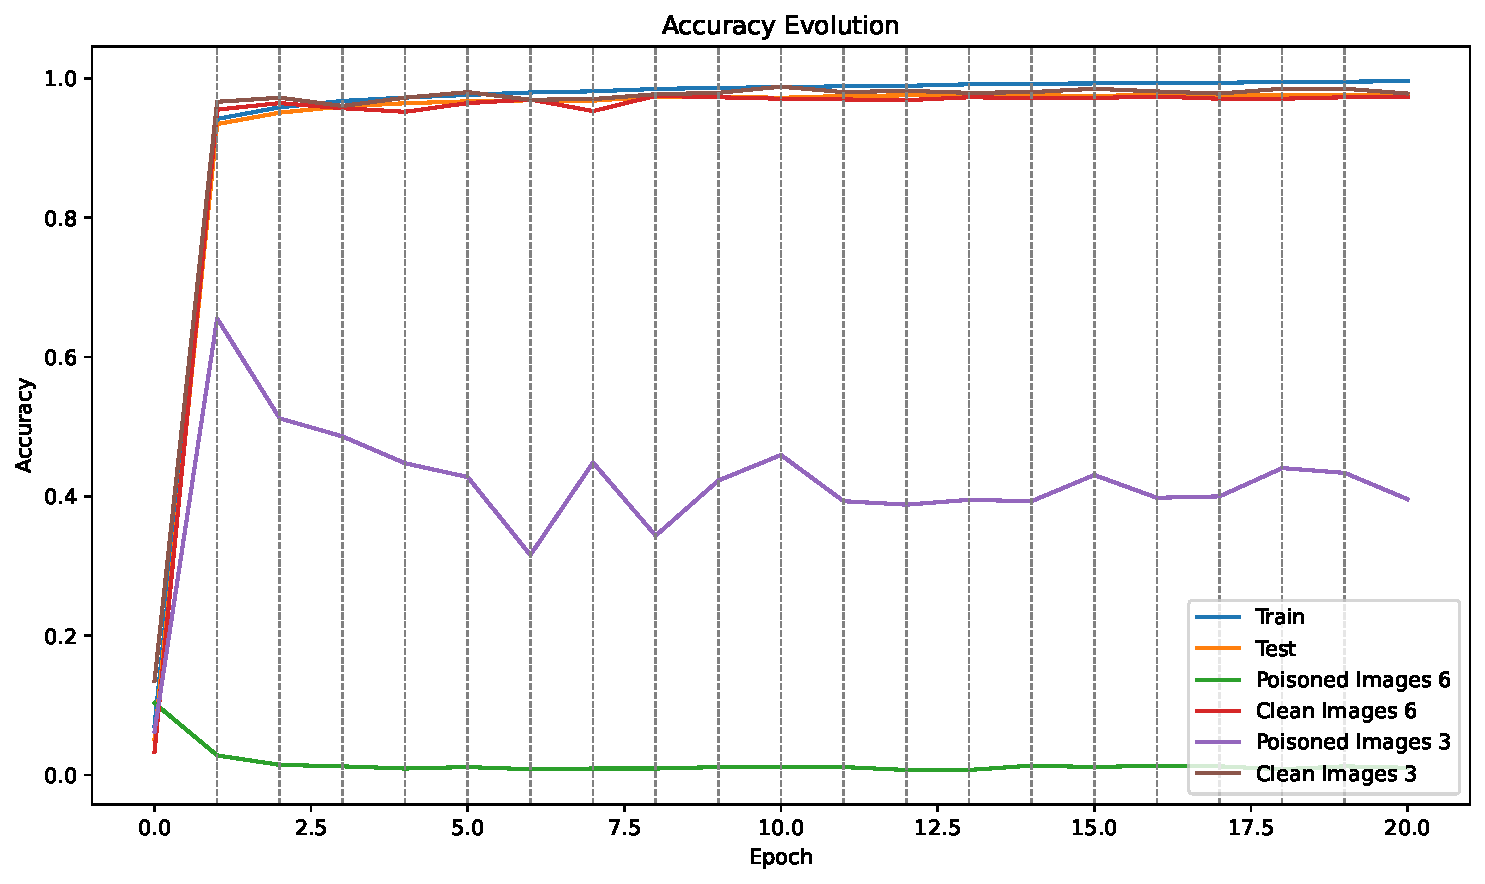
\includegraphics[width=\linewidth]{main_plots/accuracy_evolution-128-t-t-ps4.pdf}
    \caption{Accuracy}
    \label{fig:4x4acc}
\end{subfigure}
\caption{Evolution of trust mass and accuracy for a fully trusted input, MNIST poisoned experiment, patch size \(4\times4\).}
\label{fig:4x4both}
\end{figure}

All the results are depicted in Figures in \cref{sec:rescancer0.01,sec:rescancer0.1,sec:resmnistaccapp,sec:resmnist,sec:resmnistpois,sec:resrand}.
\begin{itemize}
\item \emph{Fully Trusted Input}: where the trust in the data is considered trusted (row 1 in each figure).
\item \emph{Fully Uncertain Input}: where the trust in the data is considered uncertain (row 2 in each figure).
\item \emph{Fully Distrusted Input}: where the data is assumed to be unreliable (row 3 in each figure).
\end{itemize}

% \subsection{Plots for Cancer Model with \(\epsilon = 0.01\) (\cref{exp:1})}\label{sec:rescancer0.01}

\begin{figure}[H]
  \includegraphics[width=\textwidth]{plots_v2/Cancer/eps=0.1/plot_ptas-d-d.pdf}
  \caption{xdistrust+ydistrust}
\end{figure}

\begin{figure}[H]
  
\includegraphics[width=\textwidth]{good_plots/cancer/hidden=16/eps=0.01/xdistrustyvacuous/all.pdf}
  \caption{xdistrust+yvacuous}
\end{figure}
\begin{figure}[H]
  
\includegraphics[width=\textwidth]{good_plots/cancer/hidden=16/eps=0.01/xdistrustytrust/all.pdf}
  \caption{xdistrust+ytrust}
\end{figure}
\begin{figure}[H]
  
\includegraphics[width=\textwidth]{good_plots/cancer/hidden=16/eps=0.01/xvacuousydistrust/all.pdf}
  \caption{xvacuous+ydistrust}
\end{figure}
\begin{figure}[H]
  
\includegraphics[width=\textwidth]{good_plots/cancer/hidden=16/eps=0.01/xvacuousyvacuous/all.pdf}
  \caption{xvacuous+yvacuous}
\end{figure}
\begin{figure}[H]
  
\includegraphics[width=\textwidth]{good_plots/cancer/hidden=16/eps=0.01/xvacuousytrust/all.pdf}
  \caption{xvacuous+ytrust}
\end{figure}
\begin{figure}[H]
  
\includegraphics[width=\textwidth]{good_plots/cancer/hidden=16/eps=0.01/xtrustydistrust/all.pdf}
  \caption{xtrust+ydistrust}
\end{figure}
\begin{figure}[H]
  
\includegraphics[width=\textwidth]{good_plots/cancer/hidden=16/eps=0.01/xtrustyvacuous/all.pdf}
  \caption{xtrust+yvacuous}
\end{figure}
\begin{figure}[H]
  
\includegraphics[width=\textwidth]{good_plots/cancer/hidden=16/eps=0.01/xtrustytrust/all.pdf}
  \caption{xtrust+ytrust}
\end{figure}



\subsection{Cancer Model with \( \epsilon = 0.1 \)(\cref{exp:1})}\label{sec:rescancer0.1}


\begin{figure}[H]
  
\includegraphics[width=\textwidth]{good_plots/cancer/hidden=16/eps=0.1/xdistrustydistrust/all.pdf}
  \caption{xdistrust+ydistrust}
\end{figure}
\begin{figure}[H]
  
\includegraphics[width=\textwidth]{good_plots/cancer/hidden=16/eps=0.1/xdistrustyvacuous/all.pdf}
  \caption{xdistrust+yvacuous}
\end{figure}
\begin{figure}[H]
  
\includegraphics[width=\textwidth]{good_plots/cancer/hidden=16/eps=0.1/xdistrustytrust/all.pdf}
  \caption{xdistrust+ytrust}
\end{figure}
\begin{figure}[H]
  
\includegraphics[width=\textwidth]{good_plots/cancer/hidden=16/eps=0.1/xvacuousydistrust/all.pdf}
  \caption{xvacuous+ydistrust}
\end{figure}
\begin{figure}[H]
  
\includegraphics[width=\textwidth]{good_plots/cancer/hidden=16/eps=0.1/xvacuousyvacuous/all.pdf}
  \caption{xvacuous+yvacuous}
\end{figure}
\begin{figure}[H]
  
\includegraphics[width=\textwidth]{good_plots/cancer/hidden=16/eps=0.1/xvacuousytrust/all.pdf}
  \caption{xvacuous+ytrust}
\end{figure}
\begin{figure}[H]
  
\includegraphics[width=\textwidth]{good_plots/cancer/hidden=16/eps=0.1/xtrustydistrust/all.pdf}
  \caption{xtrust+ydistrust}
\end{figure}
\begin{figure}[H]
  
\includegraphics[width=\textwidth]{good_plots/cancer/hidden=16/eps=0.1/xtrustyvacuous/all.pdf}
  \caption{xtrust+yvacuous}
\end{figure}
\begin{figure}[H]
  
\includegraphics[width=\textwidth]{good_plots/cancer/hidden=16/eps=0.1/xtrustytrust/all.pdf}
  \caption{xtrust+ytrust}
\end{figure}




\subsection{Results for trust Degradation (\cref{exp:1})}\label{sec:resdegradation}

\begin{figure}[H]
  
\includegraphics[width=\textwidth]{good_plots/cancer/hidden=16/025-0-075/all.pdf}
  \caption{(0.25, 0, 0.75)}
\end{figure}
\begin{figure}[H]
  
\includegraphics[width=\textwidth]{good_plots/cancer/hidden=16/025-025-050/all.pdf}
  \caption{(0.25, 0.25, 0.5)}
\end{figure}
    





% 


\subsection{Accuracy Evolution for the Cancer Model (\cref{exp:1})}\label{sec:resmnistaccapp}
\begin{figure}[H]
\centering
\begin{subfigure}[b]{0.32\textwidth}
  
\includegraphics[width=\textwidth]{good_plots/accuracy/Cancer/0.3-0.5/Cancer-clean-clean.pdf}
  \caption{Clean Features and Labels}
\end{subfigure}
\begin{subfigure}[b]{0.32\textwidth}
  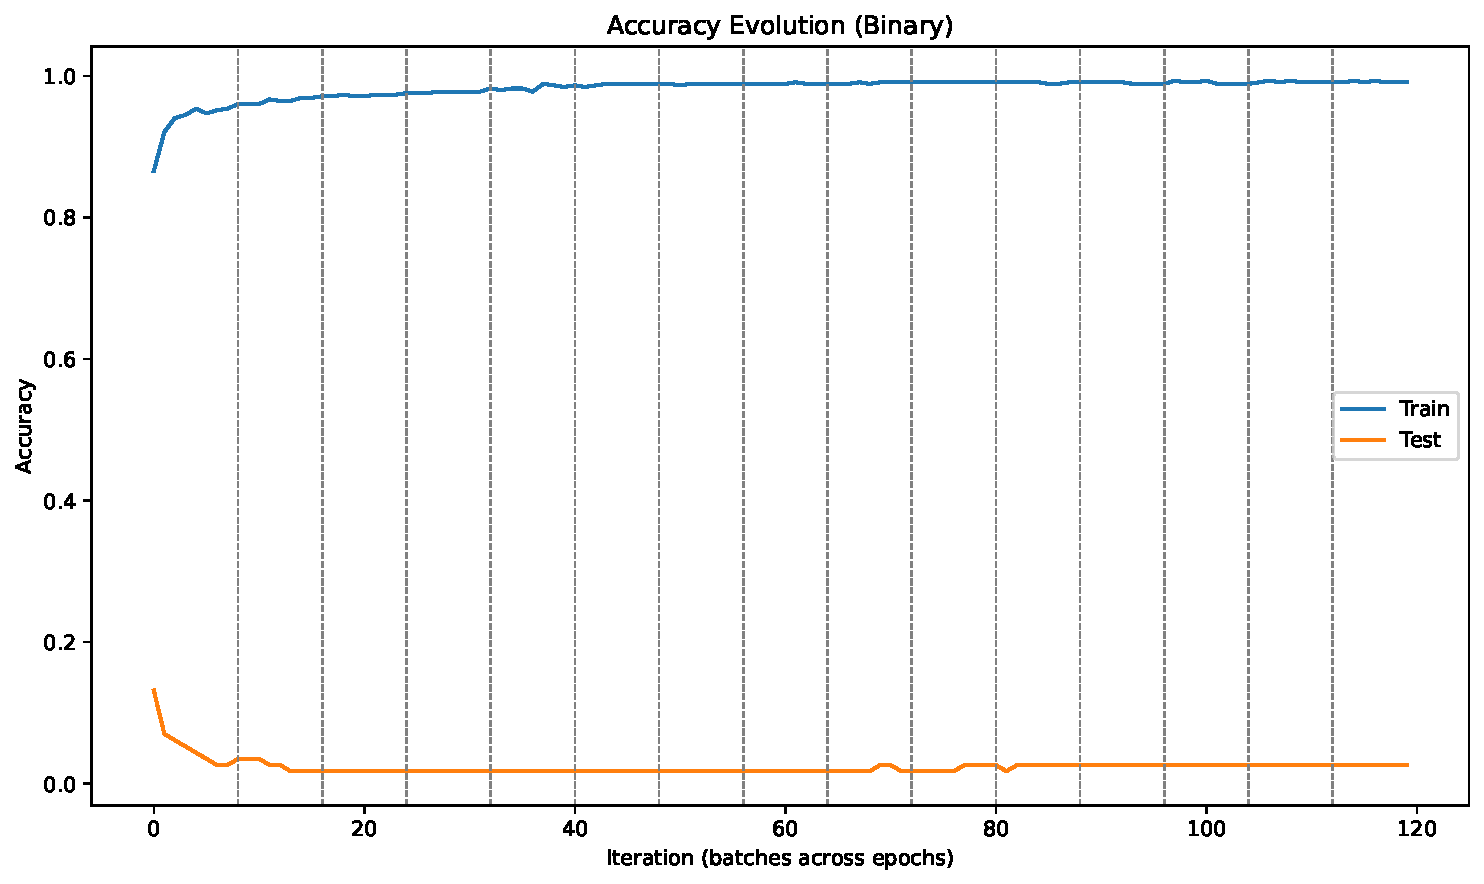
\includegraphics[width=\textwidth]{plots_v2/Cancer/eps=0.01/accuracy_evolution-t-d.pdf}
  \caption{Clean Features and Corrupted Labels}
\end{subfigure}
\begin{subfigure}[b]{0.32\textwidth}
  
\includegraphics[width=\textwidth]{good_plots/accuracy/Cancer/0.3-0.5/Cancer-clean-noise.pdf}
  \caption{Clean Features and Noisy Labels}
\end{subfigure}
\begin{subfigure}[b]{0.32\textwidth}
  
\includegraphics[width=\textwidth]{good_plots/accuracy/Cancer/0.3-0.5/Cancer-noise-clean.pdf}
  \caption{Noisy Features and Clean Labels}
\end{subfigure}
\begin{subfigure}[b]{0.32\textwidth}
  
\includegraphics[width=\textwidth]{good_plots/accuracy/Cancer/0.3-0.5/Cancer-noise-corrupt.pdf}
  \caption{Noisy Features and Corrupted Labels}
\end{subfigure}
\begin{subfigure}[b]{0.32\textwidth}
  
\includegraphics[width=\textwidth]{good_plots/accuracy/Cancer/0.3-0.5/Cancer-noise-noise.pdf}
  \caption{Noisy Features and Noisy Labels}
\end{subfigure}
\begin{subfigure}[b]{0.32\textwidth}
  
\includegraphics[width=\textwidth]{good_plots/accuracy/Cancer/0.3-0.5/Cancer-corrupt-clean.pdf}
  \caption{Corrupted Features and Clean Labels}
\end{subfigure}
\begin{subfigure}[b]{0.32\textwidth}
  
\includegraphics[width=\textwidth]{good_plots/accuracy/Cancer/0.3-0.5/Cancer-corrupt-corrupt.pdf}
  \caption{Corrupted Features and Corrupted Labels}
\end{subfigure}
\begin{subfigure}[b]{0.32\textwidth}
  
\includegraphics[width=\textwidth]{good_plots/accuracy/Cancer/0.3-0.5/Cancer-corrupt-noise.pdf}
  \caption{Corrupted Features and Noisy Labels}
\end{subfigure}
\caption{Accuracy evolution of the Cancer model under different combinations of clean, corrupted, and noisy features and labels.}
\label{fig:Acccancer}
\end{figure}

\begin{figure}[H]
    \centering
    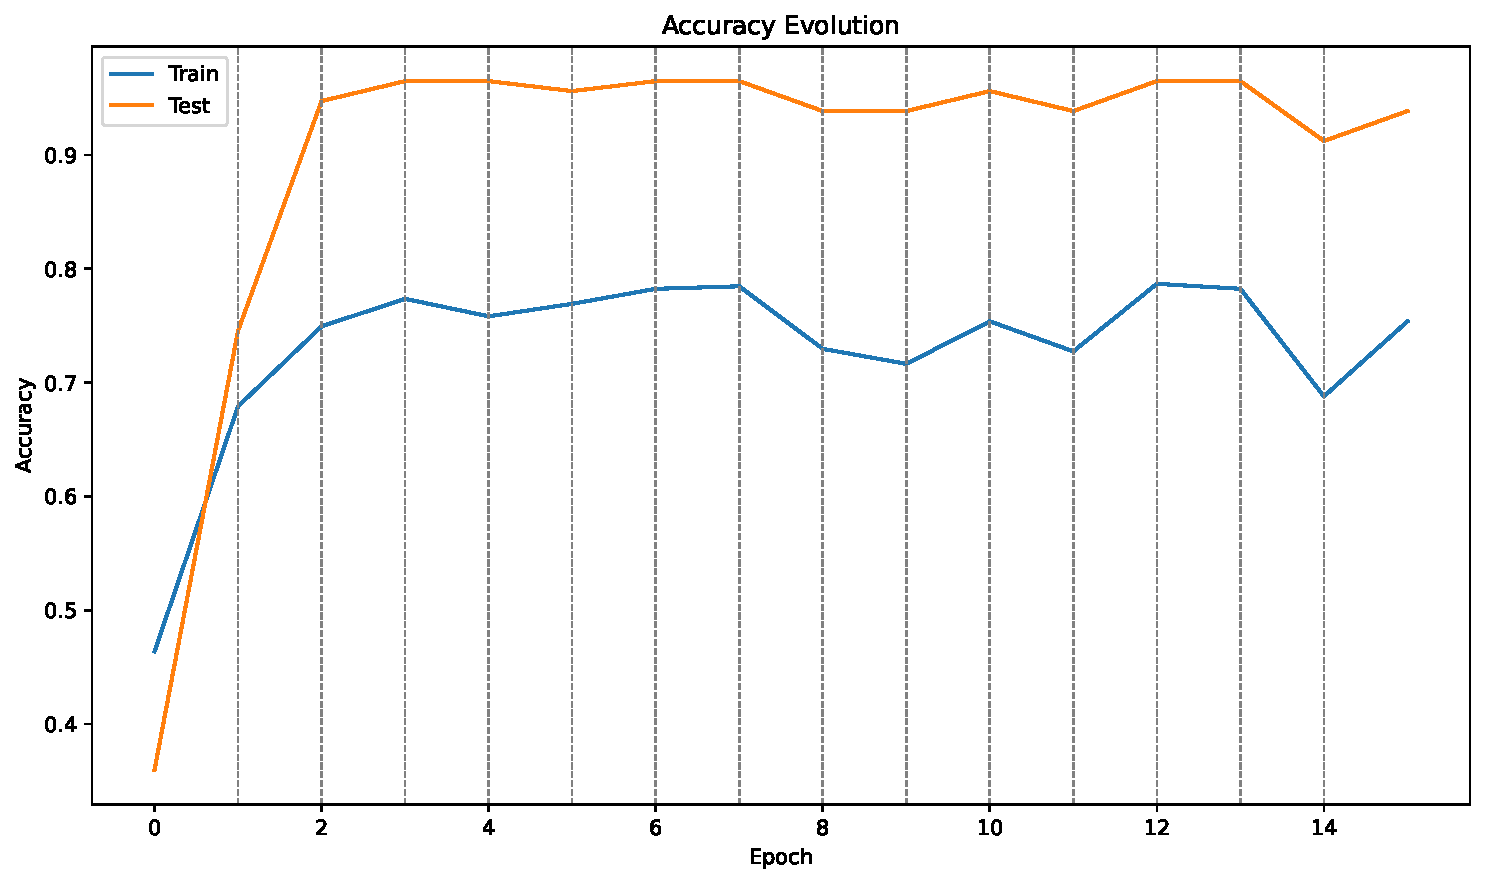
\includegraphics[width=0.8\linewidth]{good_plots/accuracy/Cancer/0.15-0.25/Cancer-noise-noise.pdf}
    \caption{Accuracy evolution of the Cancer model when reducing the noise for noised features and labels.}
    \label{fig:AcccancerInt}
\end{figure}





% \subsection{MNIST with Vacuous Trust Assessment (\cref{exp:2})}\label{sec:resmnist}
% \begin{figure}[H]
%   \centering
%   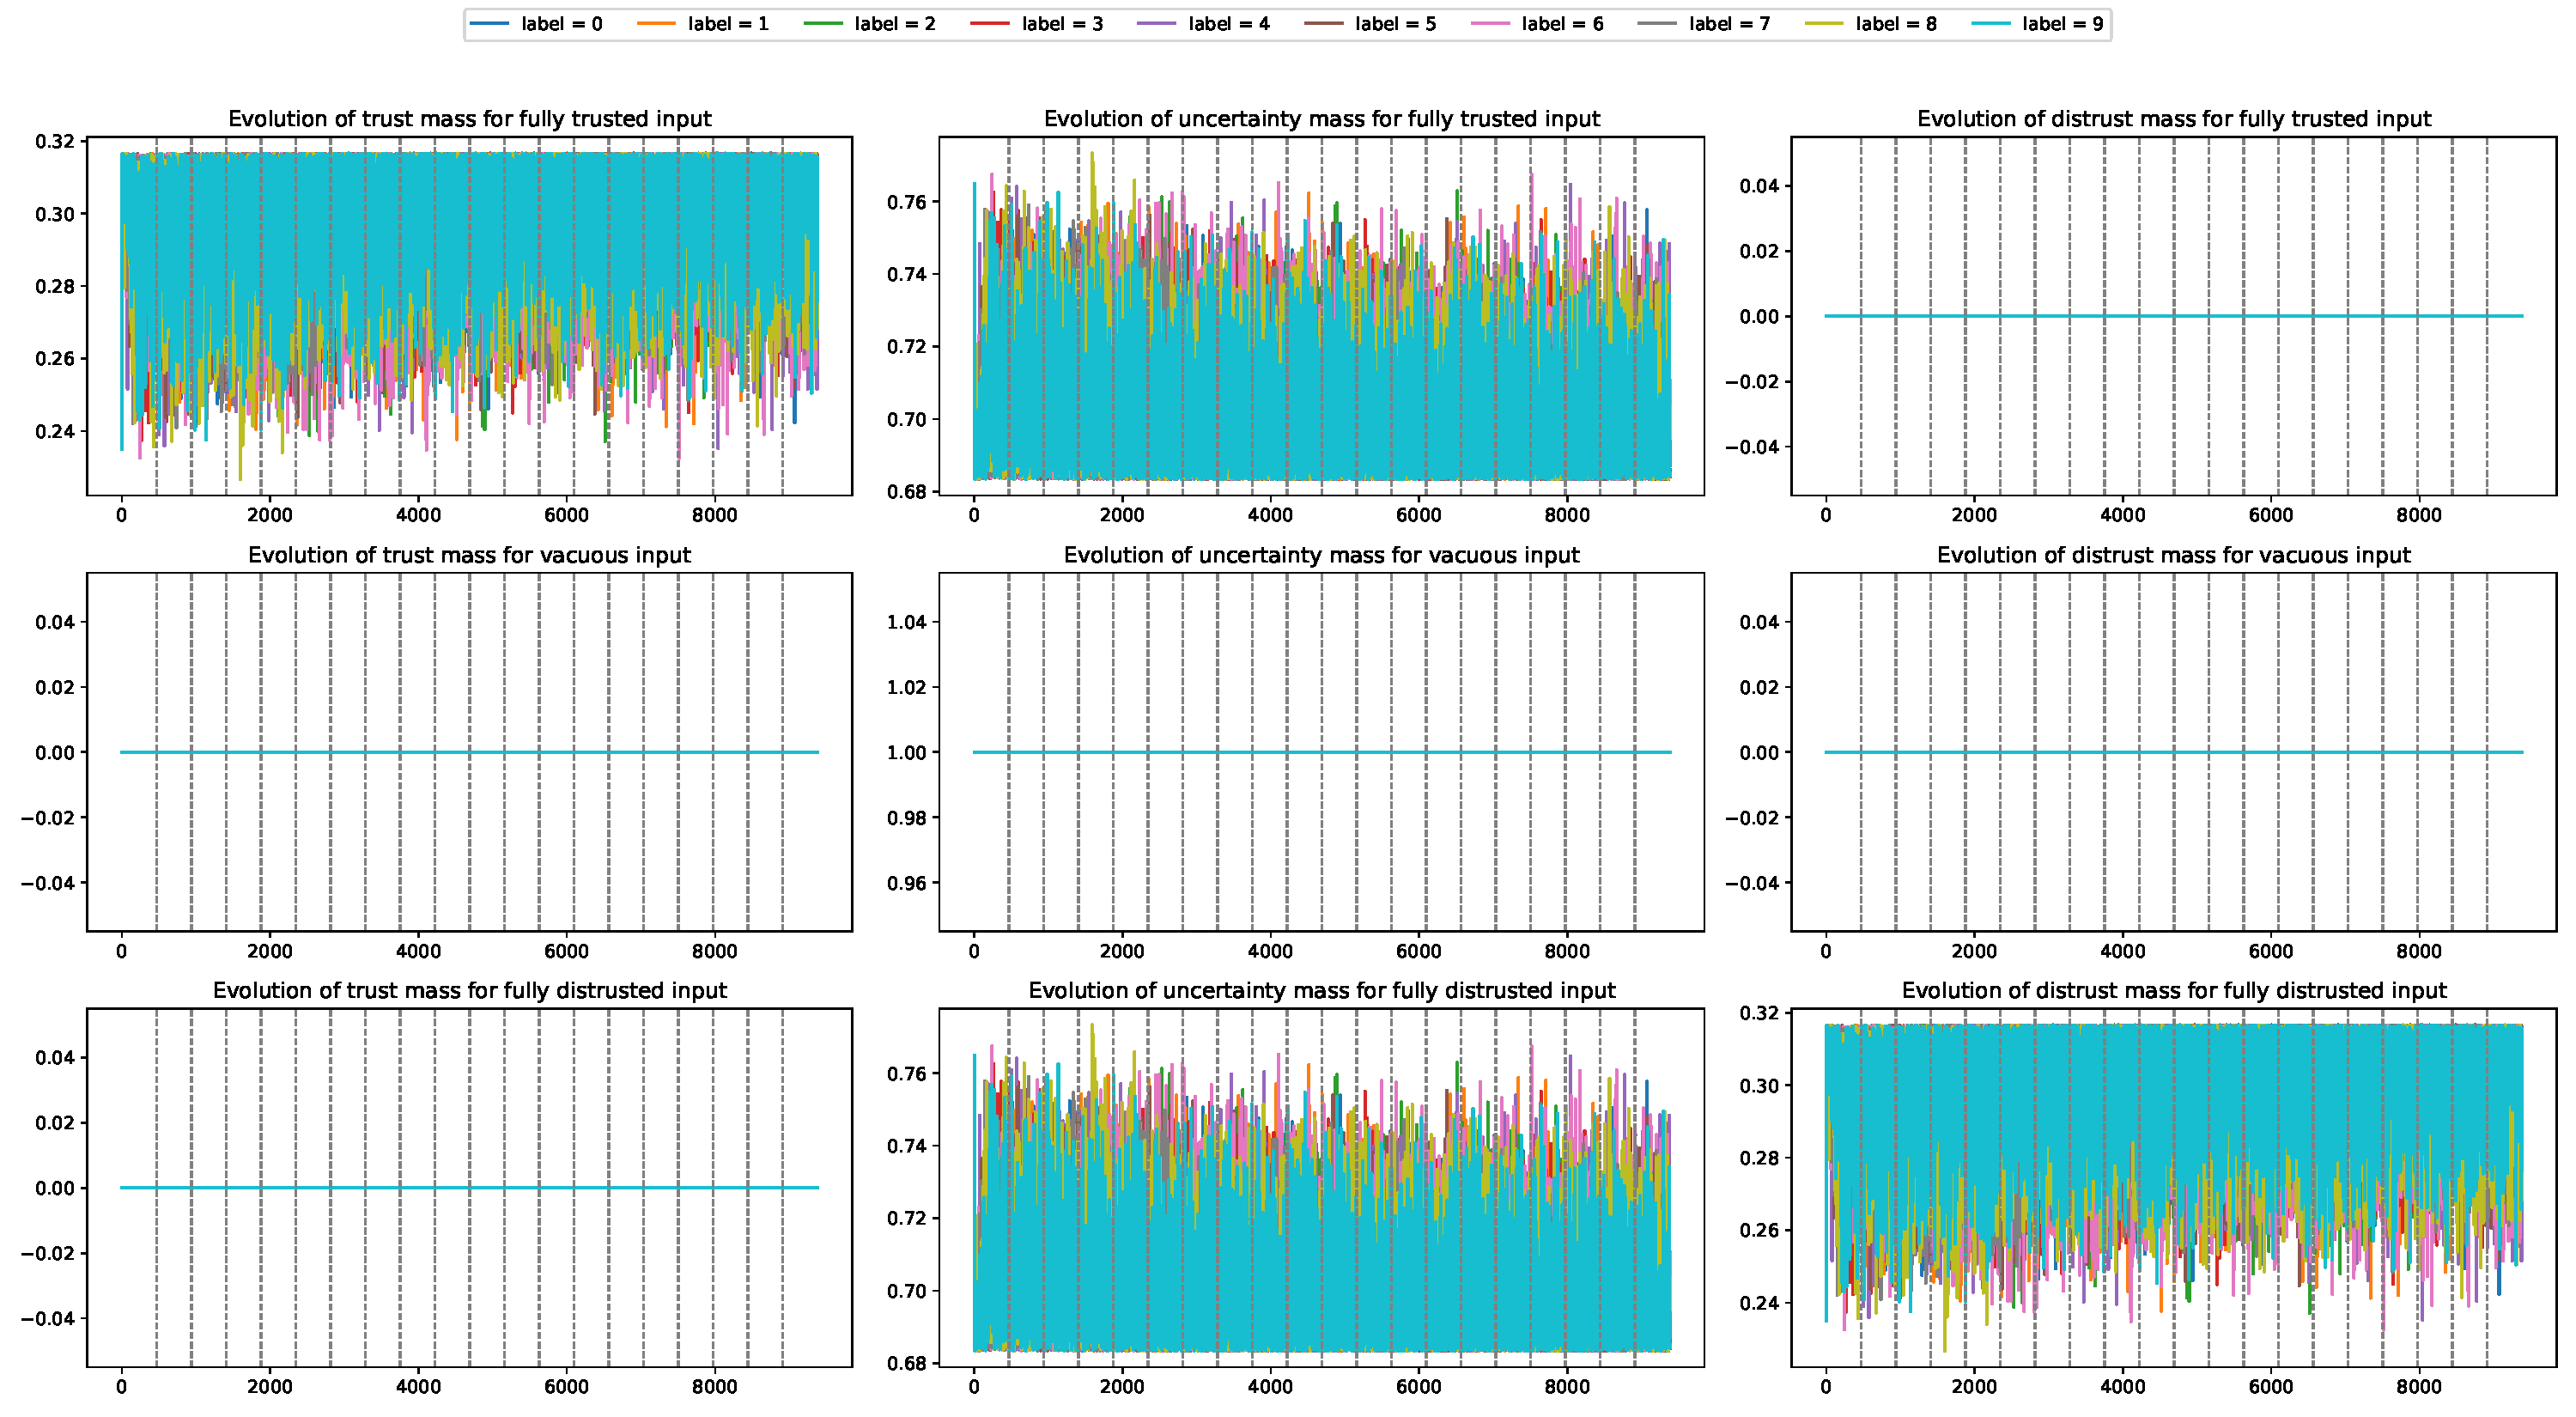
\includegraphics[width=\textwidth]{plots_v2/MNIST/architecture/plot_ptas-16-v-v.pdf}
%   \caption{16 Hidden neurons}
% \end{figure}
% \begin{figure}[H]
%   \centering
%   
\includegraphics[width=\textwidth]{good_plots/MNIST/hidden=20/xvacuousyvacuous/all.pdf}
%   \caption{20 Hidden neurons}
% \end{figure}
% \begin{figure}[H]
%   \centering
%   
\includegraphics[width=\textwidth]{good_plots/MNIST/hidden=20/xtrustytrust/all.pdf}
%   \caption{20 Hidden neurons with Fully Trusted Assessment}
% \end{figure}



% \begin{figure}[H]
% \centering
% \begin{subfigure}[b]{0.49\textwidth}
%   \centering
%   
\includegraphics[width=\textwidth]{good_plots/accuracy/MNIST/hiddenSize/5.pdf}
%   \caption{5 Hidden neurons}
% \end{subfigure}
% \begin{subfigure}[b]{0.49\textwidth}
%   \centering
%   
\includegraphics[width=\textwidth]{good_plots/accuracy/MNIST/hiddenSize/10.pdf}
%   \caption{10 Hidden neurons}
% \end{subfigure}
% \begin{subfigure}[b]{0.49\textwidth}
%   \centering
%   
\includegraphics[width=\textwidth]{good_plots/accuracy/MNIST/hiddenSize/20.pdf}
%   \caption{20 Hidden neurons}
% \end{subfigure}
% \begin{subfigure}[b]{0.49\textwidth}
%   \centering
%   
\includegraphics[width=\textwidth]{good_plots/accuracy/MNIST/hiddenSize/20T.pdf}
%   \caption{20 Hidden neurons with Fully Trusted Assessment}
% \end{subfigure}
% \caption{MNIST with Vacuous Trust Assessment}
% \label{fig:mnist}
% \end{figure}

% \subsection{MNIST poisoned 128 hidden neurons (\cref{exp:3})}\label{sec:resmnistpois}
% \begin{figure}[H]
%   \centering
%   
\includegraphics[width=\textwidth]{good_plots/MNIST/pois_hidden=20/1/all.pdf}
%   \caption{1 pixel}
% \end{figure}
% \begin{figure}[H]
%   \centering
%   
\includegraphics[width=\textwidth]{good_plots/MNIST/pois_hidden=20/4/all.pdf}
%   \caption{4×4 pixels}
% \end{figure}

% \begin{figure}[H]
%   \centering
%   
\includegraphics[width=\textwidth]{good_plots/MNIST/pois_hidden=20/20/all.pdf}
%   \caption{20×20 pixels}
% \end{figure}
% \begin{figure}[H]
%   \centering
%   
\includegraphics[width=\textwidth]{good_plots/MNIST/pois_hidden=20/27/all.pdf}
%   \caption{27×27 pixels}
% \end{figure}



% \begin{figure}[H]
% \centering
% \begin{subfigure}{0.5\textwidth}
%   \centering
%   
\includegraphics[width=\textwidth]{good_plots/accuracy/MNIST/poisoned/MNIST1.pdf}
%   \caption{1 pixel}
% \end{subfigure}
% \begin{subfigure}{0.5\textwidth}
%   \centering
%   
\includegraphics[width=\textwidth]{good_plots/accuracy/MNIST/poisoned/MNIST4.pdf}
%   \caption{4×4 pixels}
% \end{subfigure}
% \\
% \begin{subfigure}{0.5\textwidth}
%   \centering
%   
\includegraphics[width=\textwidth]{good_plots/accuracy/MNIST/poisoned/MNIST20.pdf}
%   \caption{20×20 pixels}
% \end{subfigure}
% \begin{subfigure}{0.5\textwidth}
%   \centering
%   
\includegraphics[width=\textwidth]{good_plots/accuracy/MNIST/poisoned/MNIST27.pdf}
%   \caption{27×27 pixels}
% \end{subfigure}
% \caption{Accuracy for poisoned MNIST model with 20 hidden neurons}
% \label{fig:mnistpoisacc}
% \end{figure}



\subsection{Plots for Cancer Model with \(\epsilon = 0.01\) (\cref{exp:1})}\label{sec:rescancer0.01}
\begin{figure}[H]
  \includegraphics[width=\textwidth]{plots_v2/Cancer/eps=0.01/plot_ptas-d-d.pdf}
  \caption{Features distrusted and labels distrusted}
\end{figure}
\begin{figure}[H]
  \includegraphics[width=\textwidth]{plots_v2/Cancer/eps=0.01/plot_ptas-d-v.pdf}
  \caption{Features distrusted and labels vacuous}
\end{figure}
\begin{figure}[H]
  \includegraphics[width=\textwidth]{plots_v2/Cancer/eps=0.01/plot_ptas-d-t.pdf}
  \caption{Features distrusted and labels trusted}
\end{figure}
\begin{figure}[H]
  \includegraphics[width=\textwidth]{plots_v2/Cancer/eps=0.01/plot_ptas-v-d.pdf}
  \caption{Features vacuous and labels distrusted}
\end{figure}
\begin{figure}[H]
  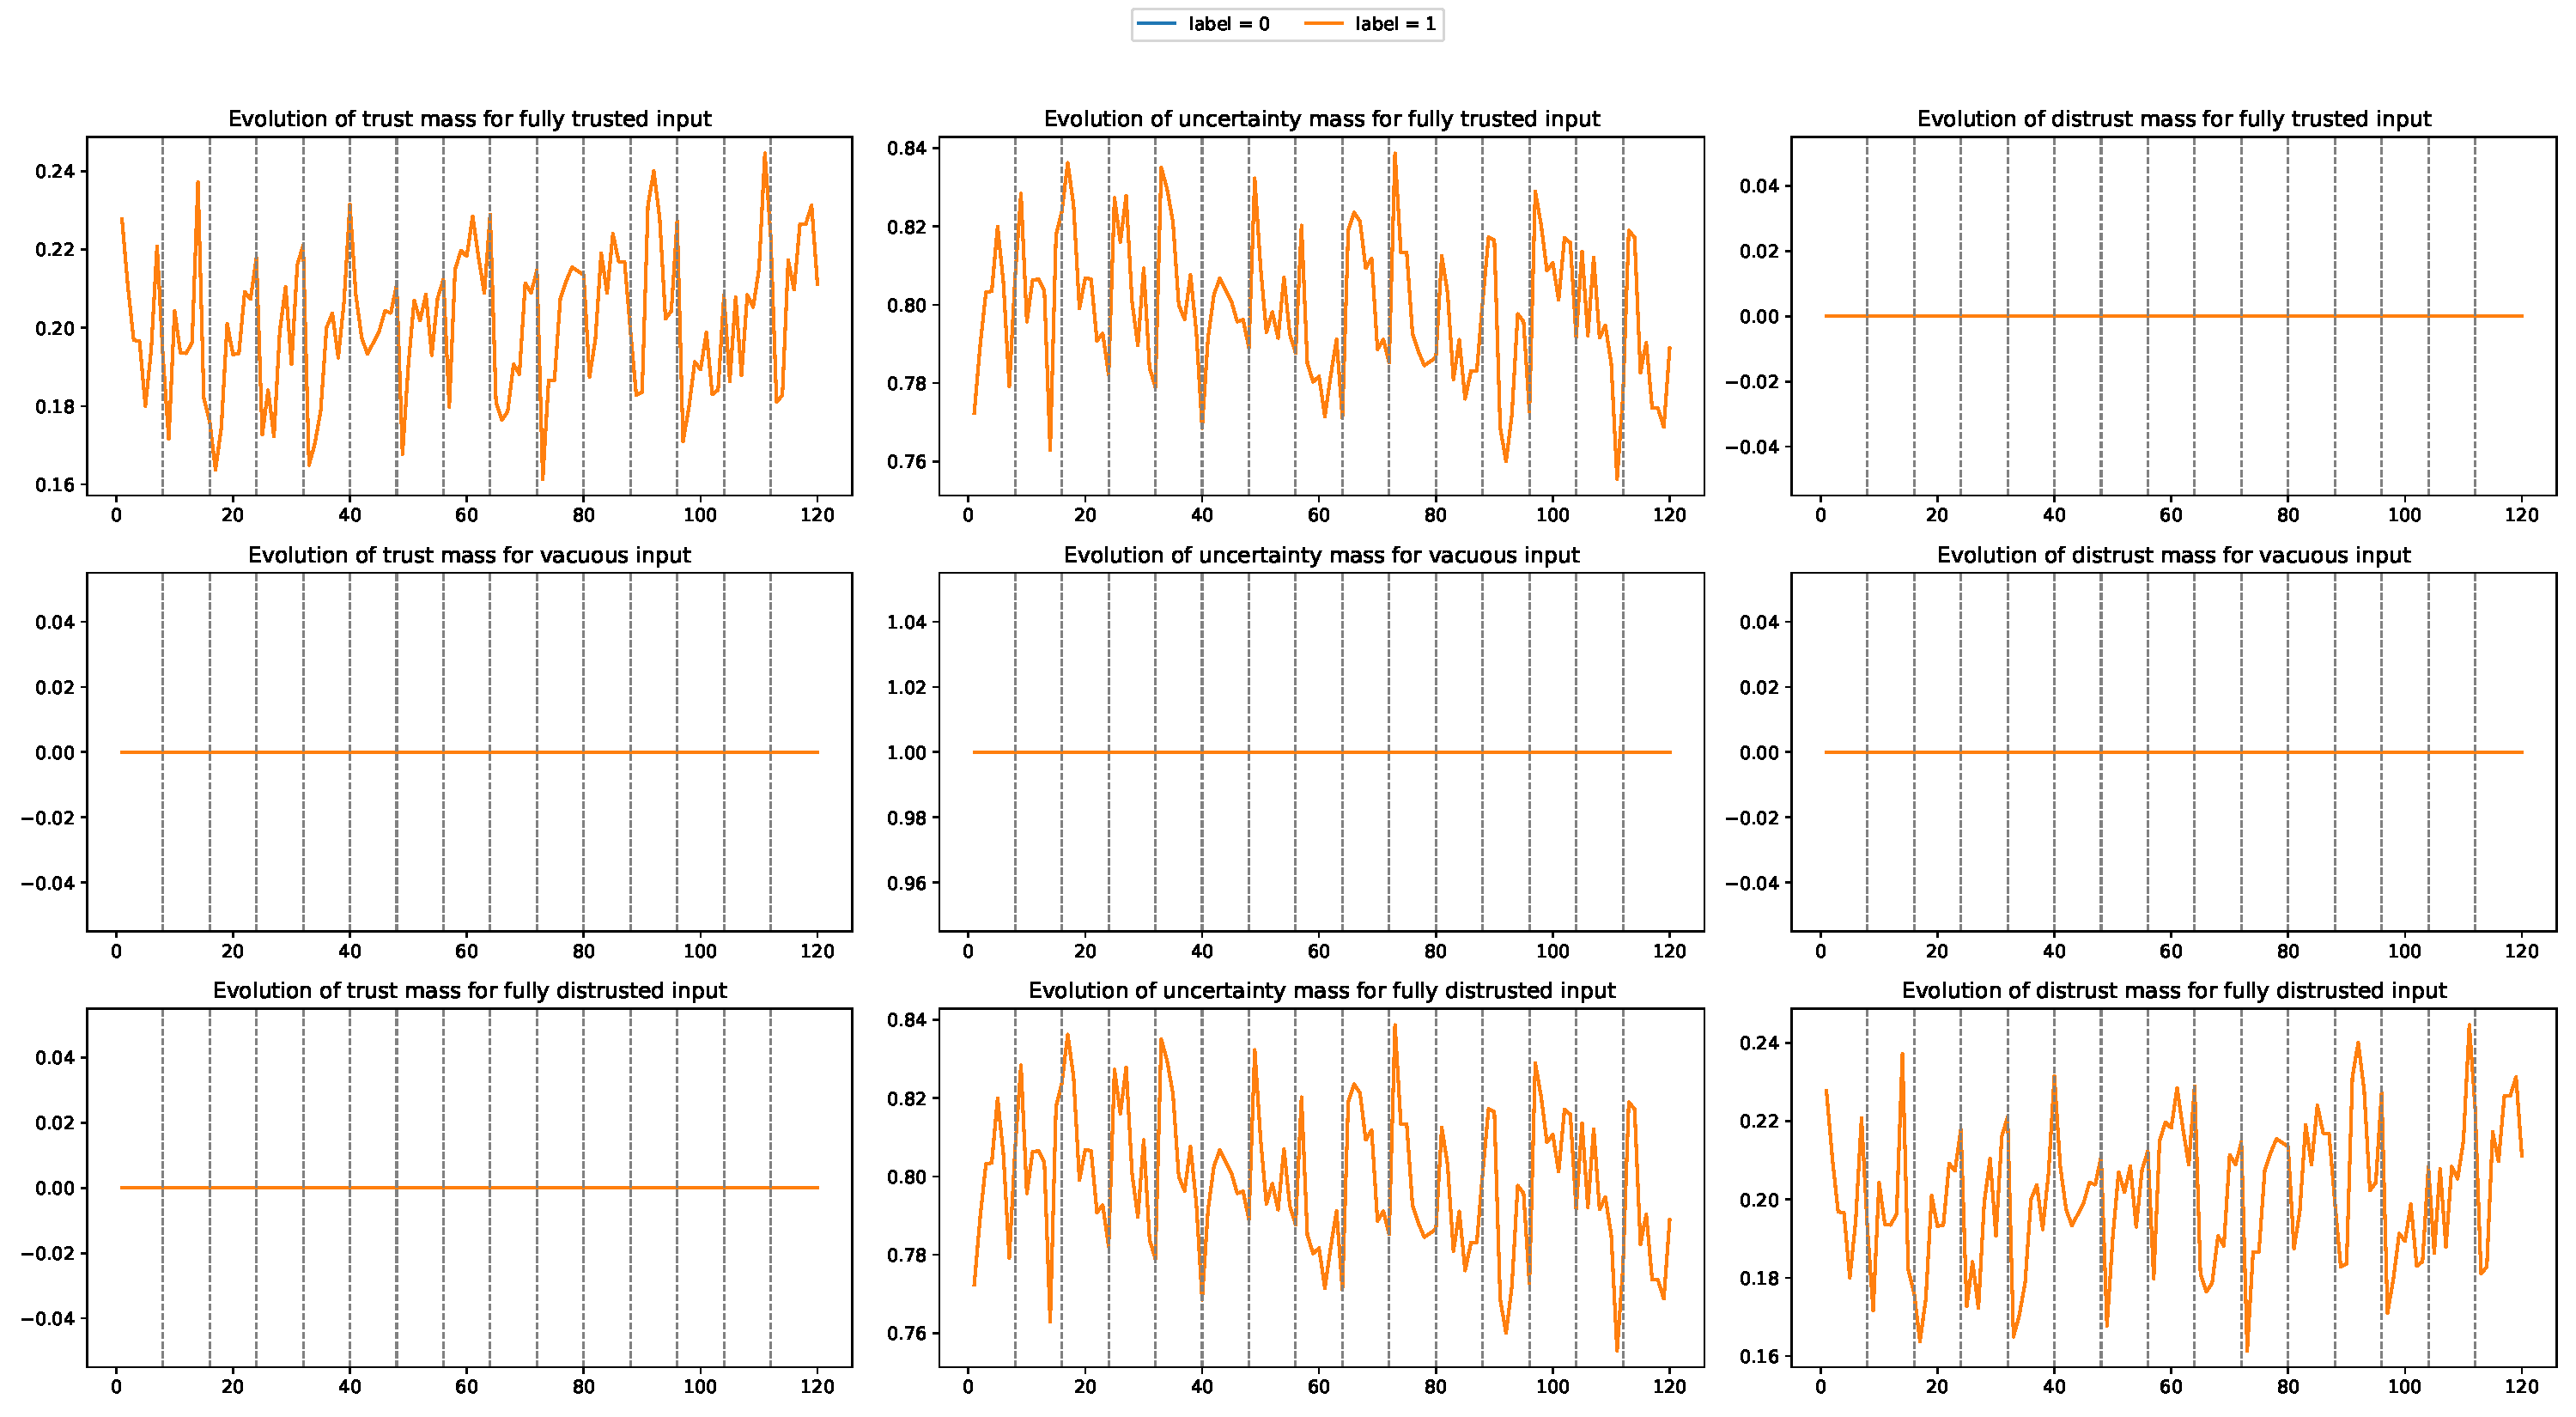
\includegraphics[width=\textwidth]{plots_v2/Cancer/eps=0.01/plot_ptas-v-v.pdf}
  \caption{Features vacuous and labels vacuous}
\end{figure}
\begin{figure}[H]
  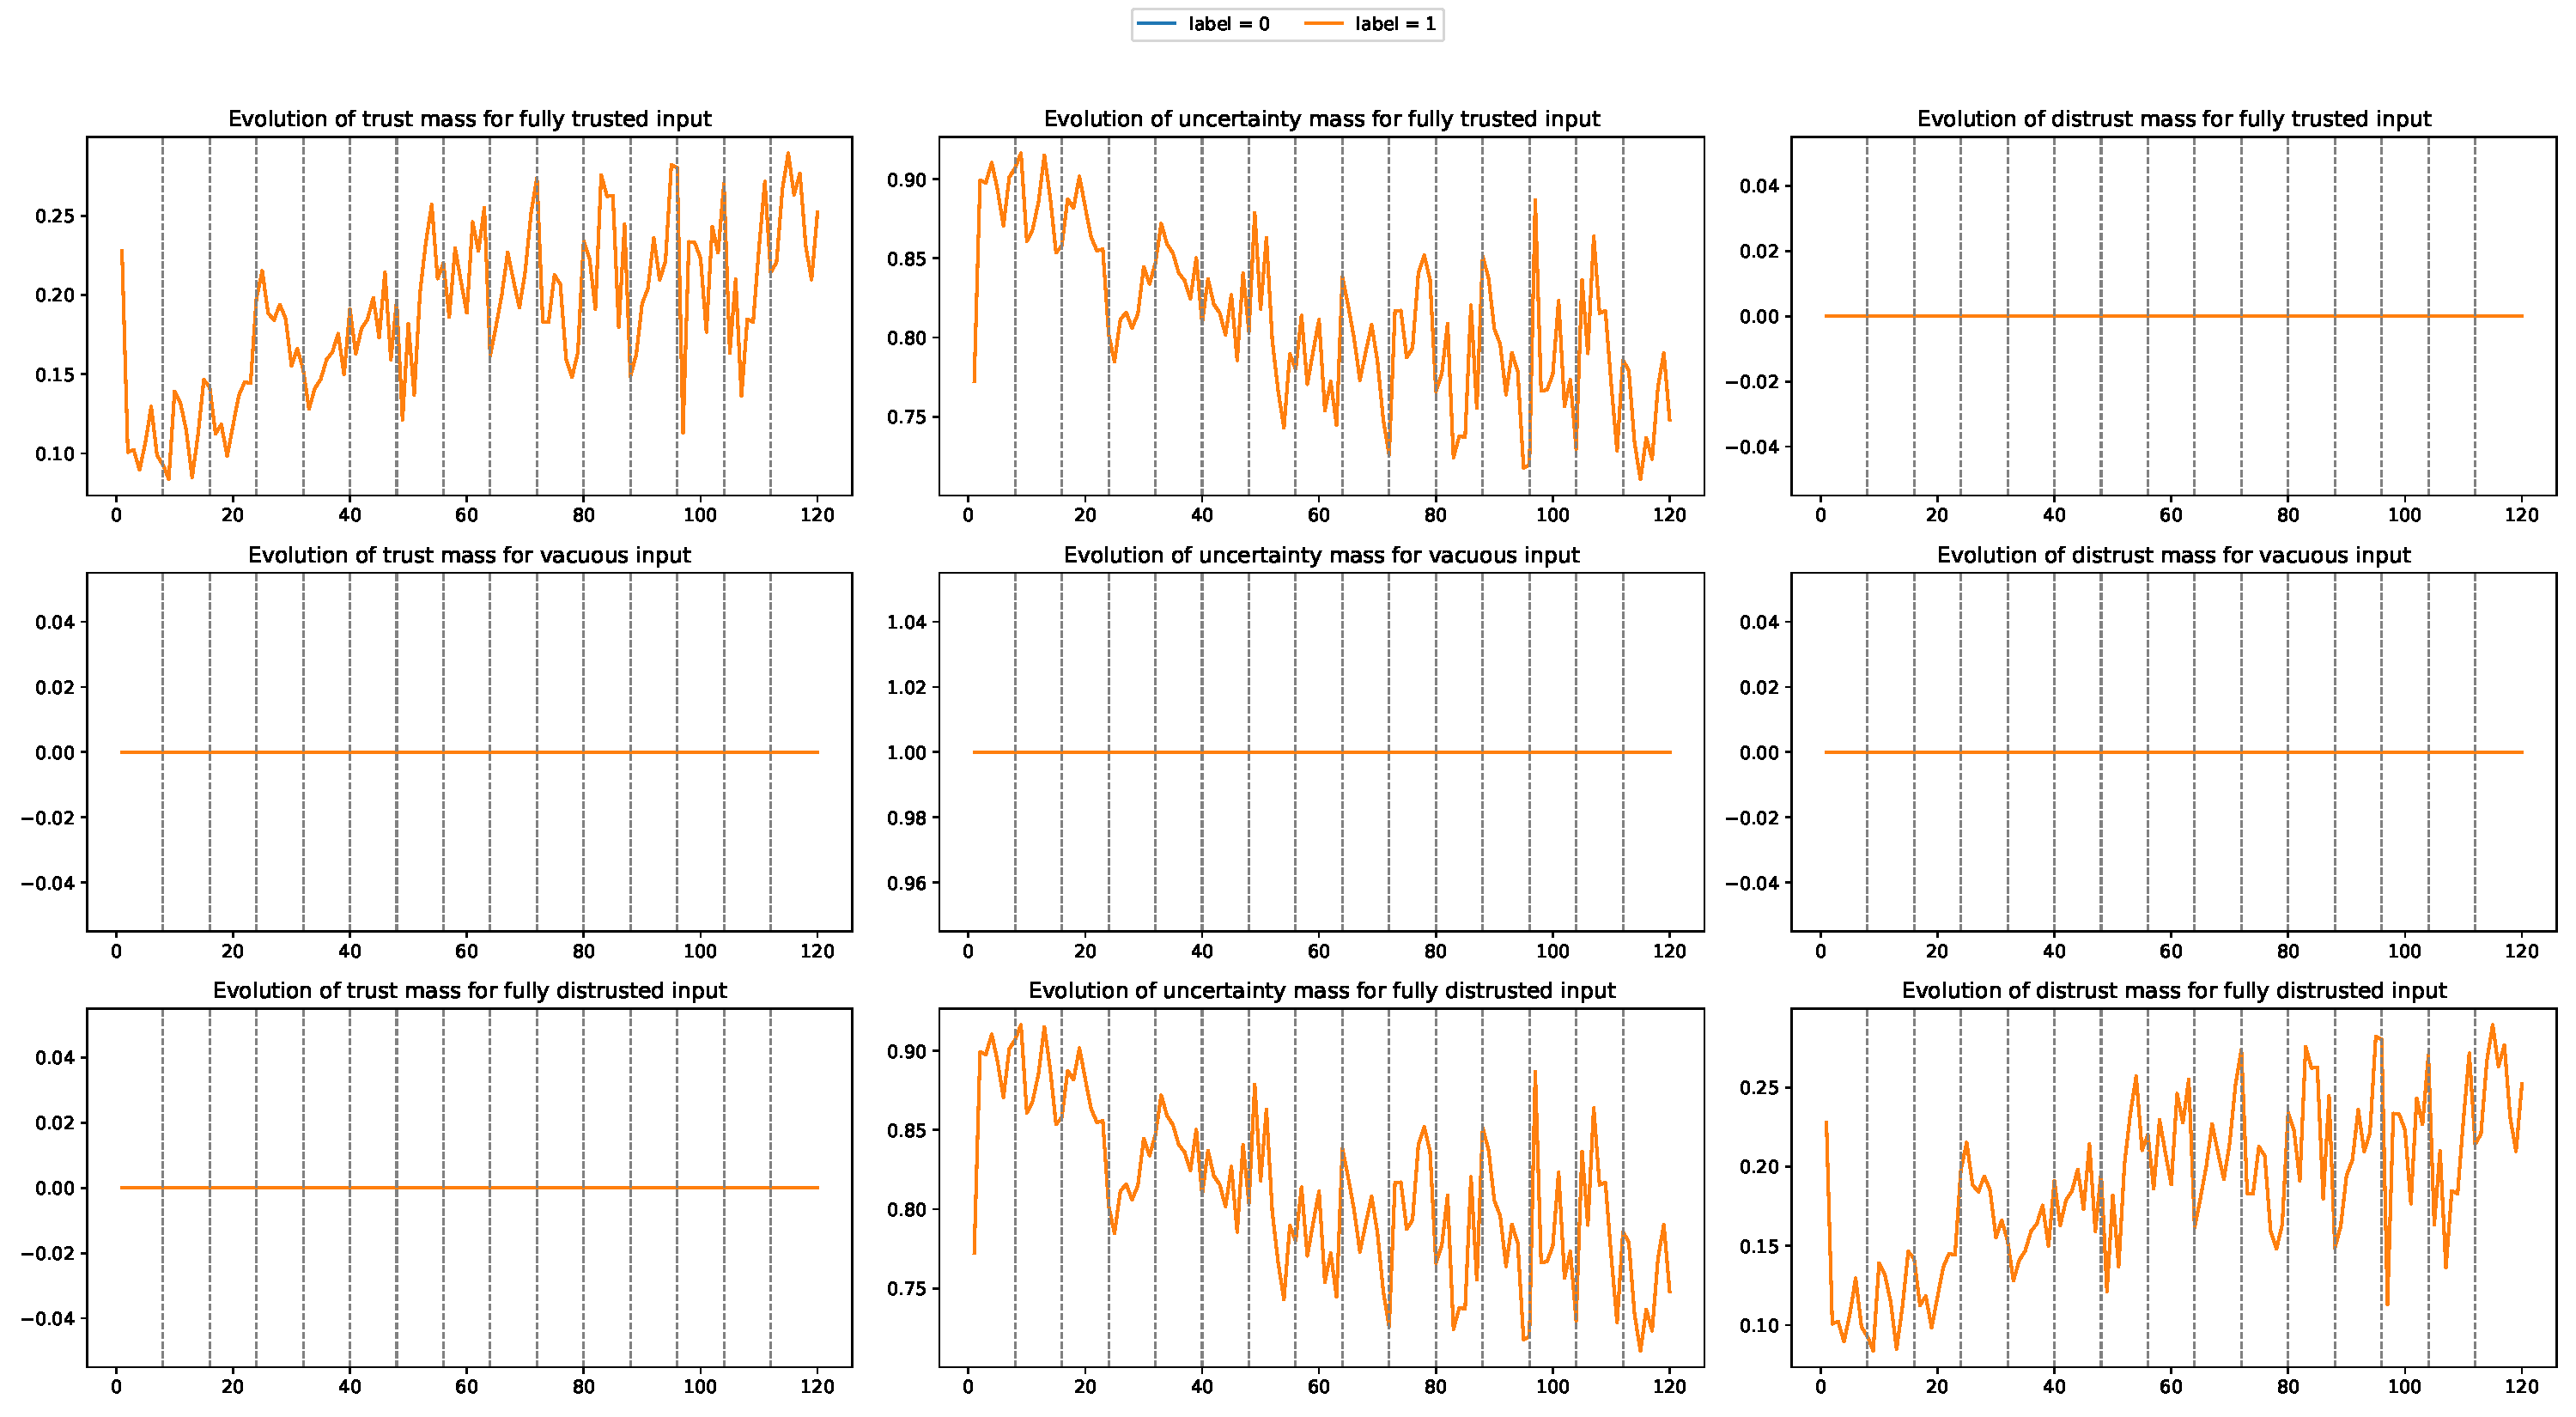
\includegraphics[width=\textwidth]{plots_v2/Cancer/eps=0.01/plot_ptas-v-t.pdf}
  \caption{Features vacuous and labels trusted}
\end{figure}
\begin{figure}[H]
  \includegraphics[width=\textwidth]{plots_v2/Cancer/eps=0.01/plot_ptas-t-d.pdf}
  \caption{Features trusted and labels distrusted}
\end{figure}
\begin{figure}[H]
  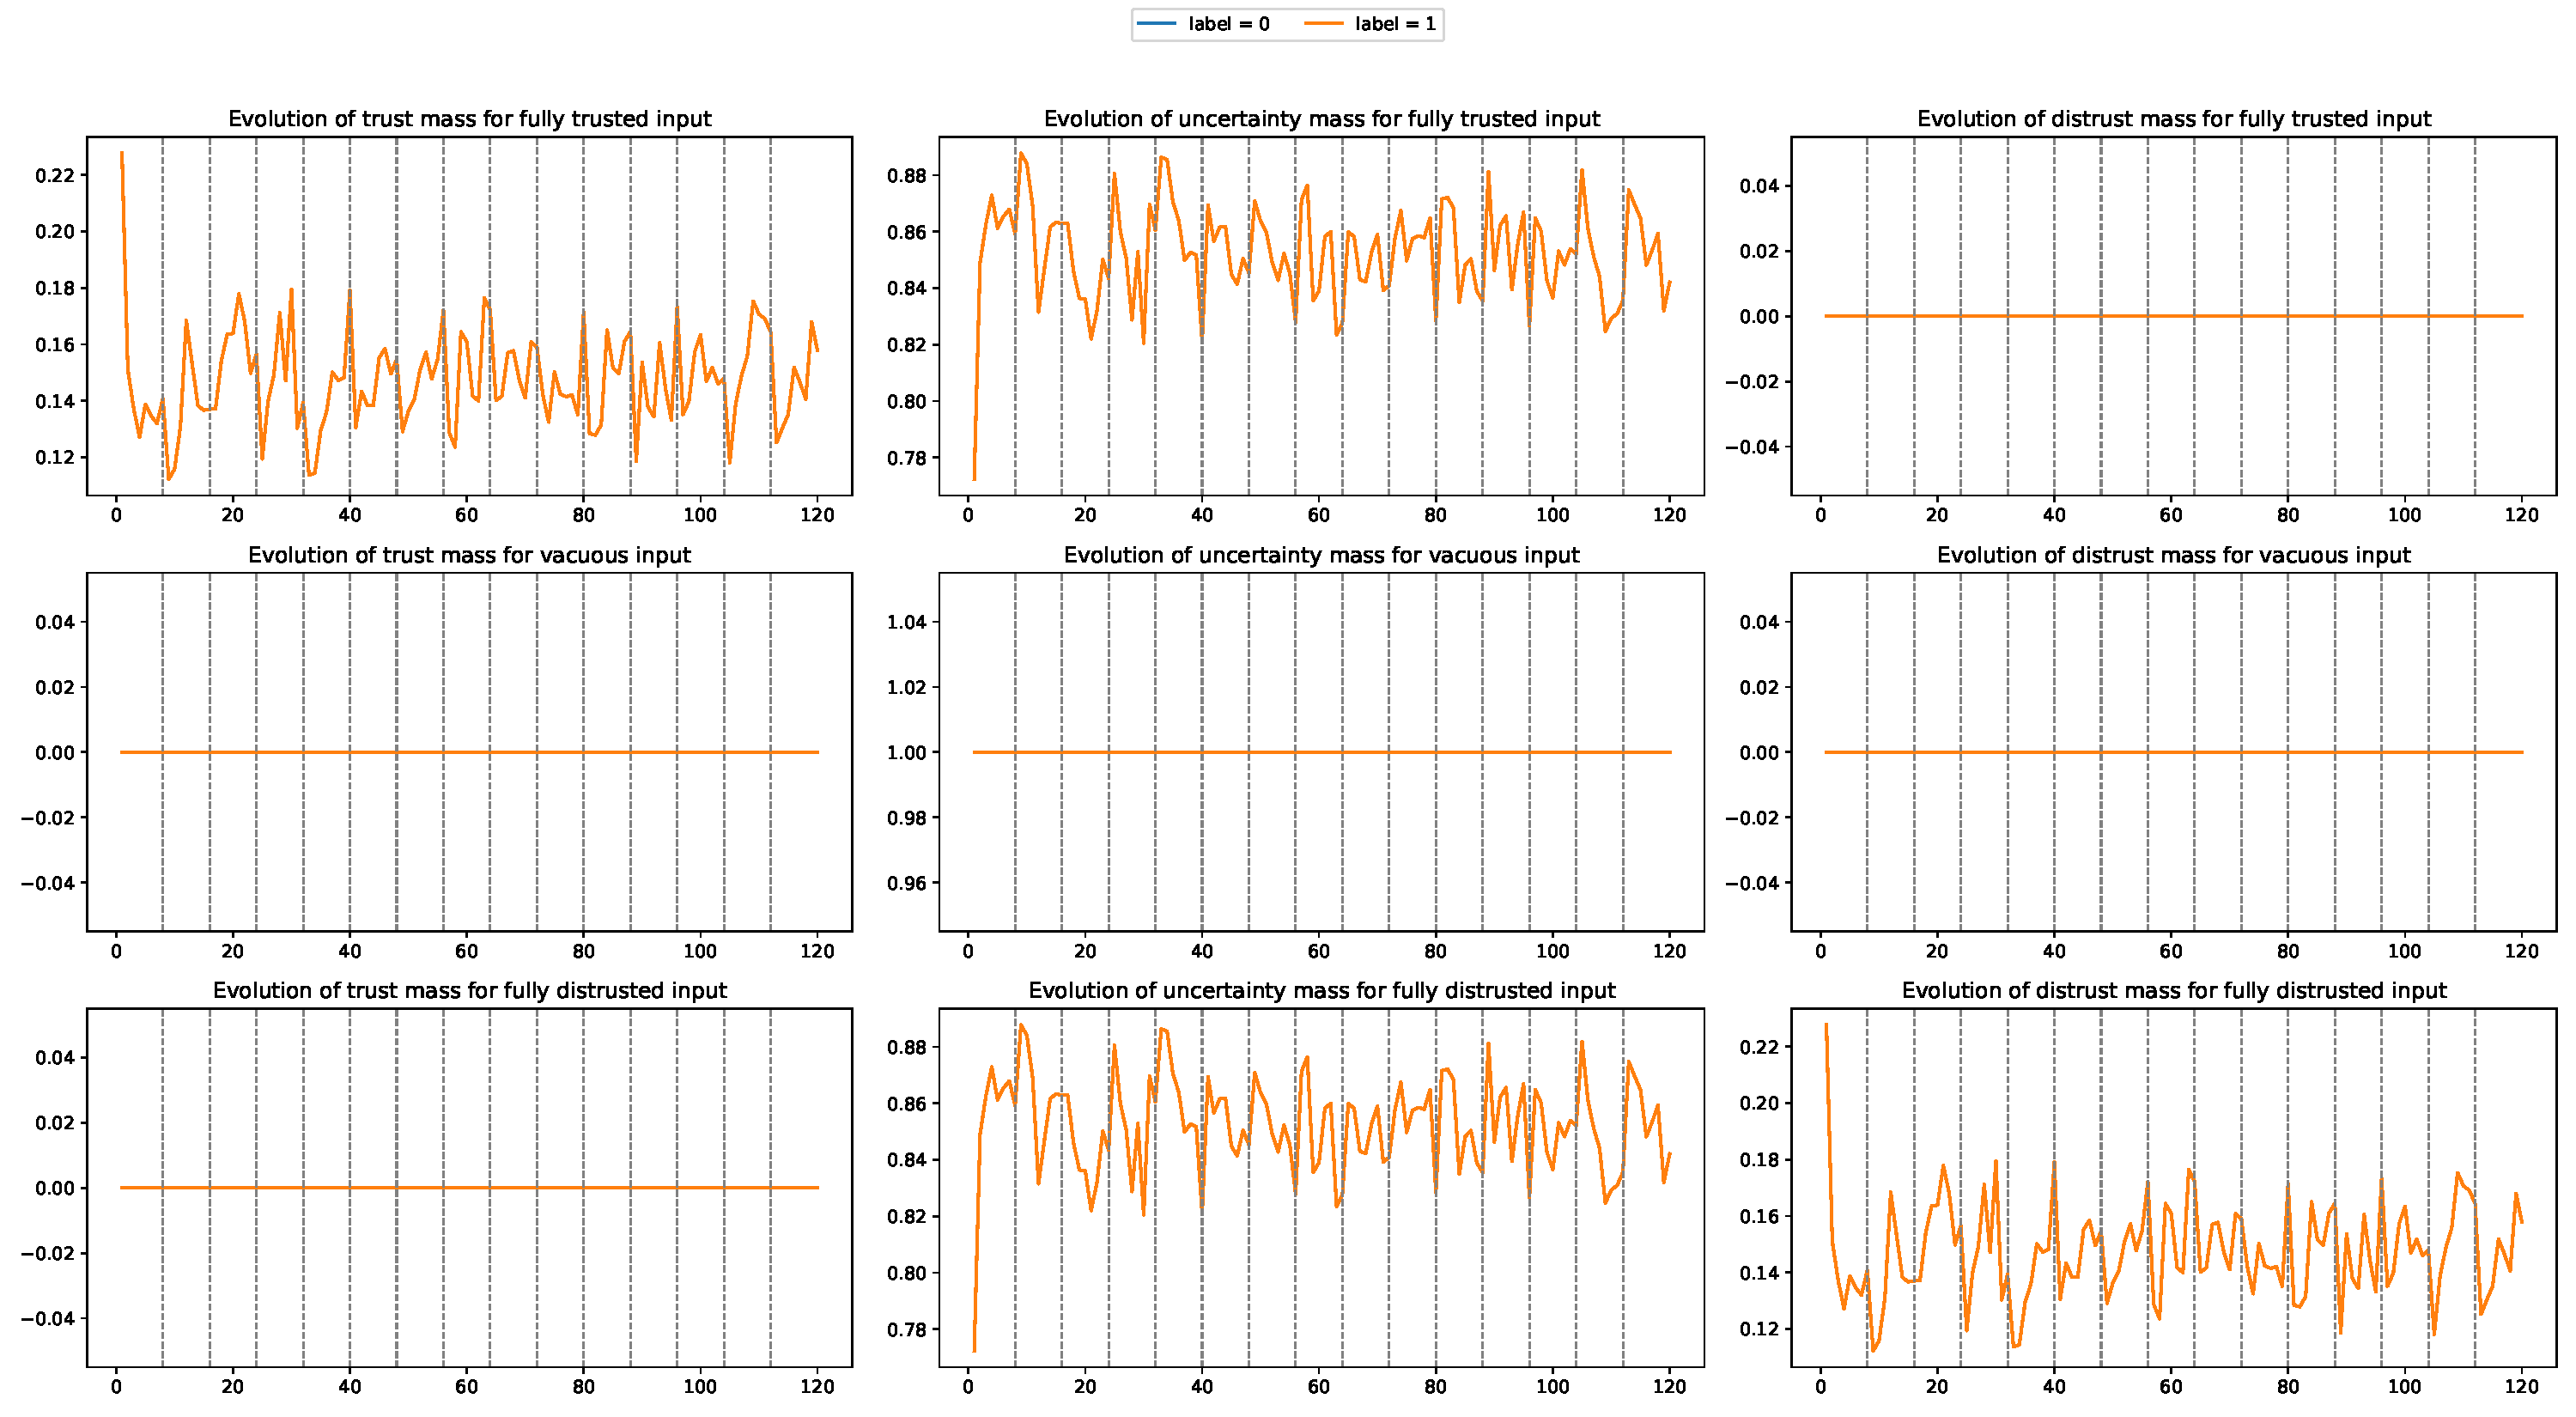
\includegraphics[width=\textwidth]{plots_v2/Cancer/eps=0.01/plot_ptas-t-v.pdf}
  \caption{Features trusted and labels vacuous}
\end{figure}
\begin{figure}[H]
  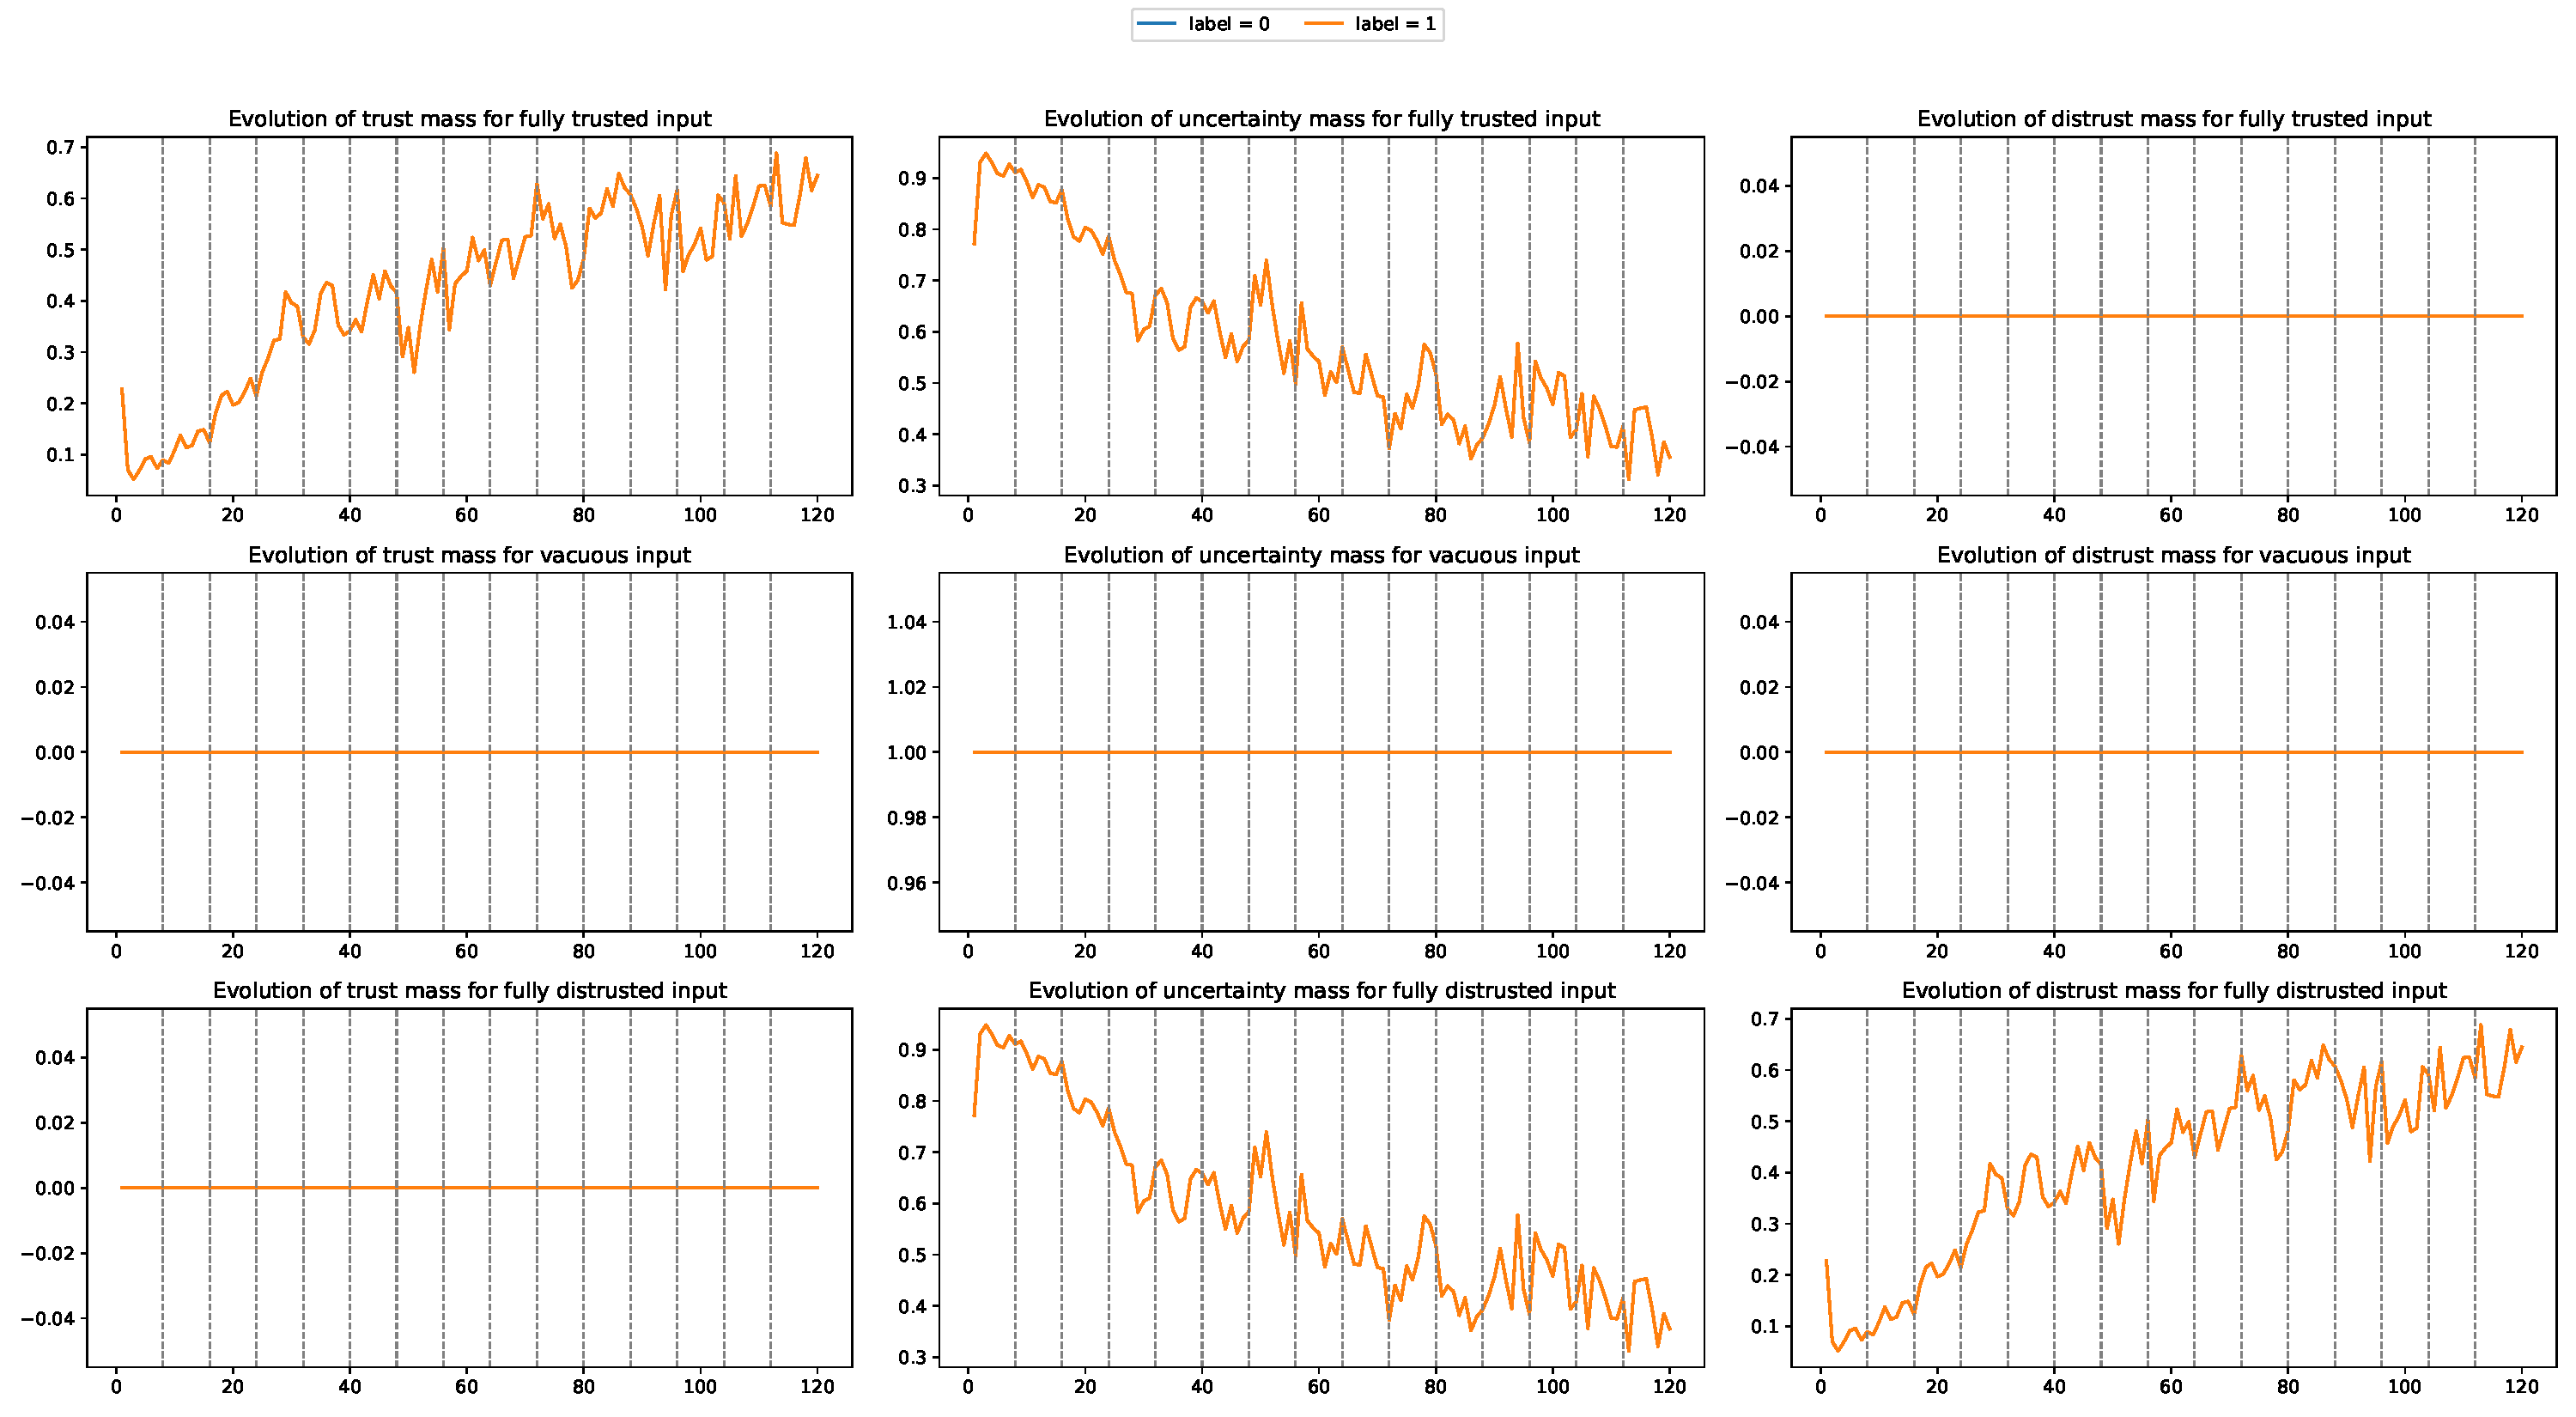
\includegraphics[width=\textwidth]{plots_v2/Cancer/eps=0.01/plot_ptas-t-t.pdf}
  \caption{Features trusted and labels trusted}
\end{figure}

\subsection{Cancer Model with \( \epsilon = 0.1 \)(\cref{exp:1})}\label{sec:rescancer0.1}
\begin{figure}[H]
  \includegraphics[width=\textwidth]{plots_v2/Cancer/eps=0.1/plot_ptas-d-d.pdf}
  \caption{Features distrusted and labels distrusted}
\end{figure}
\begin{figure}[H]
  \includegraphics[width=\textwidth]{plots_v2/Cancer/eps=0.1/plot_ptas-d-v.pdf}
  \caption{Features distrusted and labels vacuous}
\end{figure}
\begin{figure}[H]
  \includegraphics[width=\textwidth]{plots_v2/Cancer/eps=0.1/plot_ptas-d-t.pdf}
  \caption{Features distrusted and labels trusted}
\end{figure}
\begin{figure}[H]
  \includegraphics[width=\textwidth]{plots_v2/Cancer/eps=0.1/plot_ptas-v-d.pdf}
  \caption{Features vacuous and labels distrusted}
\end{figure}
\begin{figure}[H]
  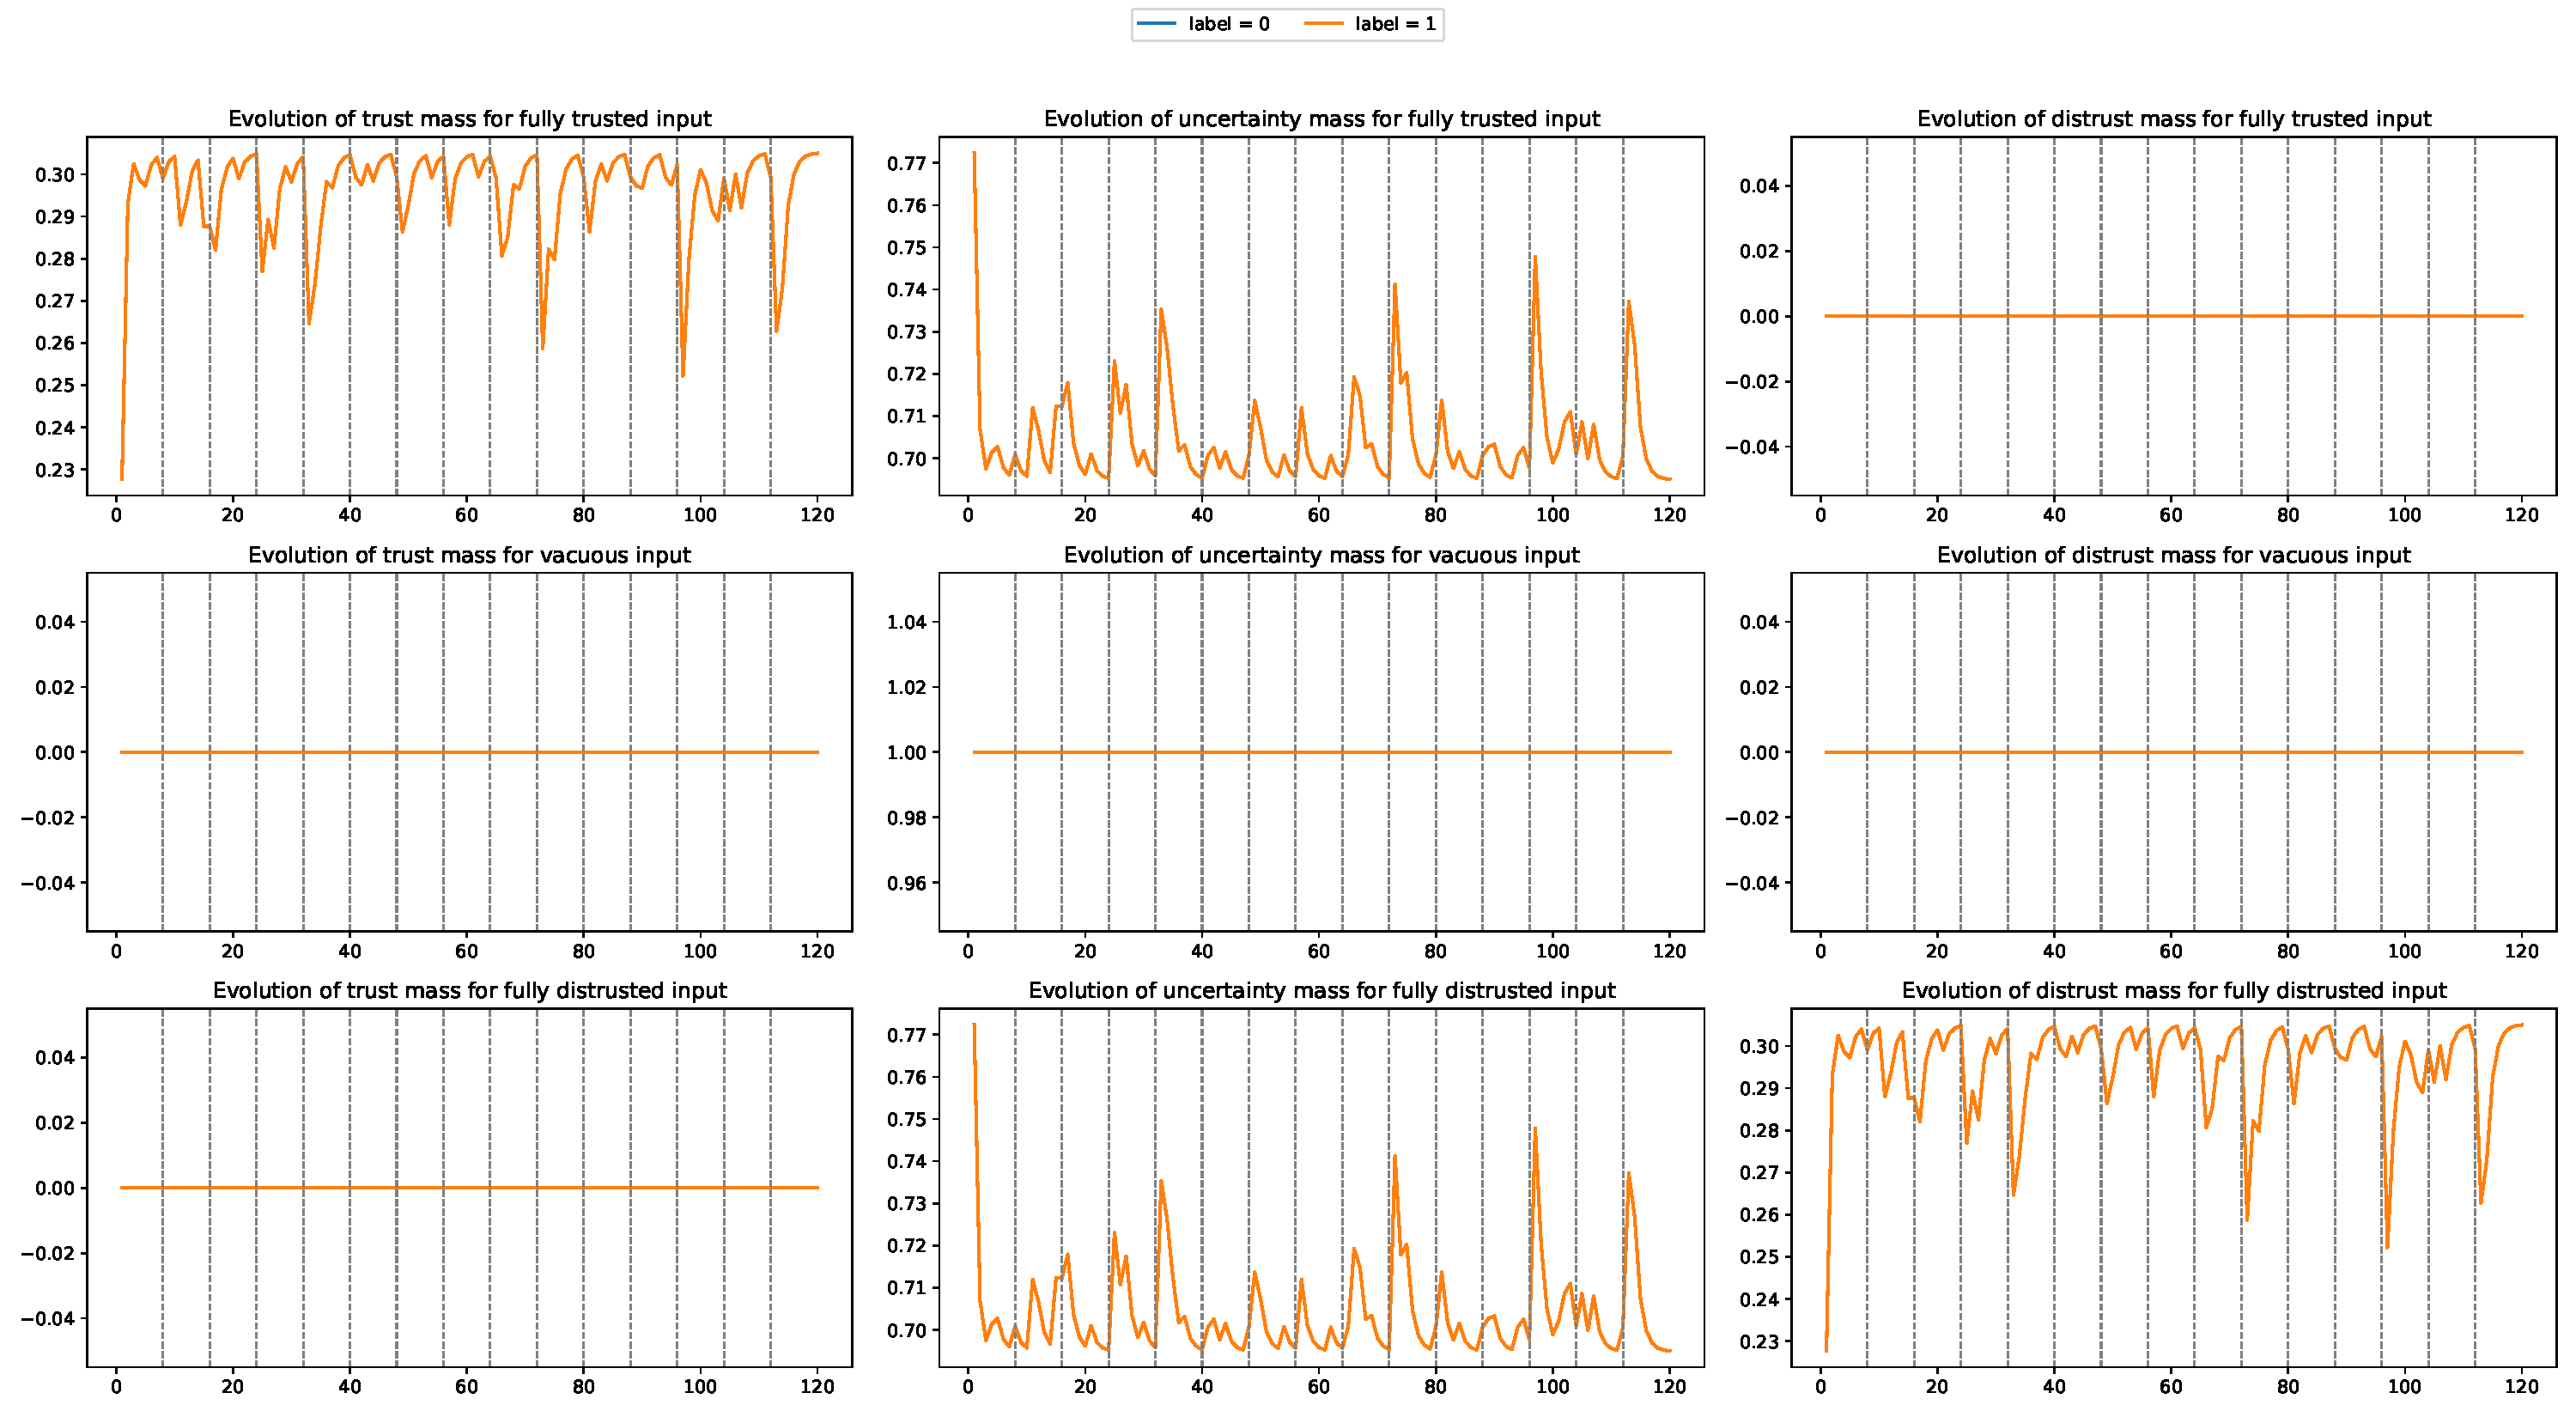
\includegraphics[width=\textwidth]{plots_v2/Cancer/eps=0.1/plot_ptas-v-v.pdf}
  \caption{Features vacuous and labels vacuous}
\end{figure}
\begin{figure}[H]
  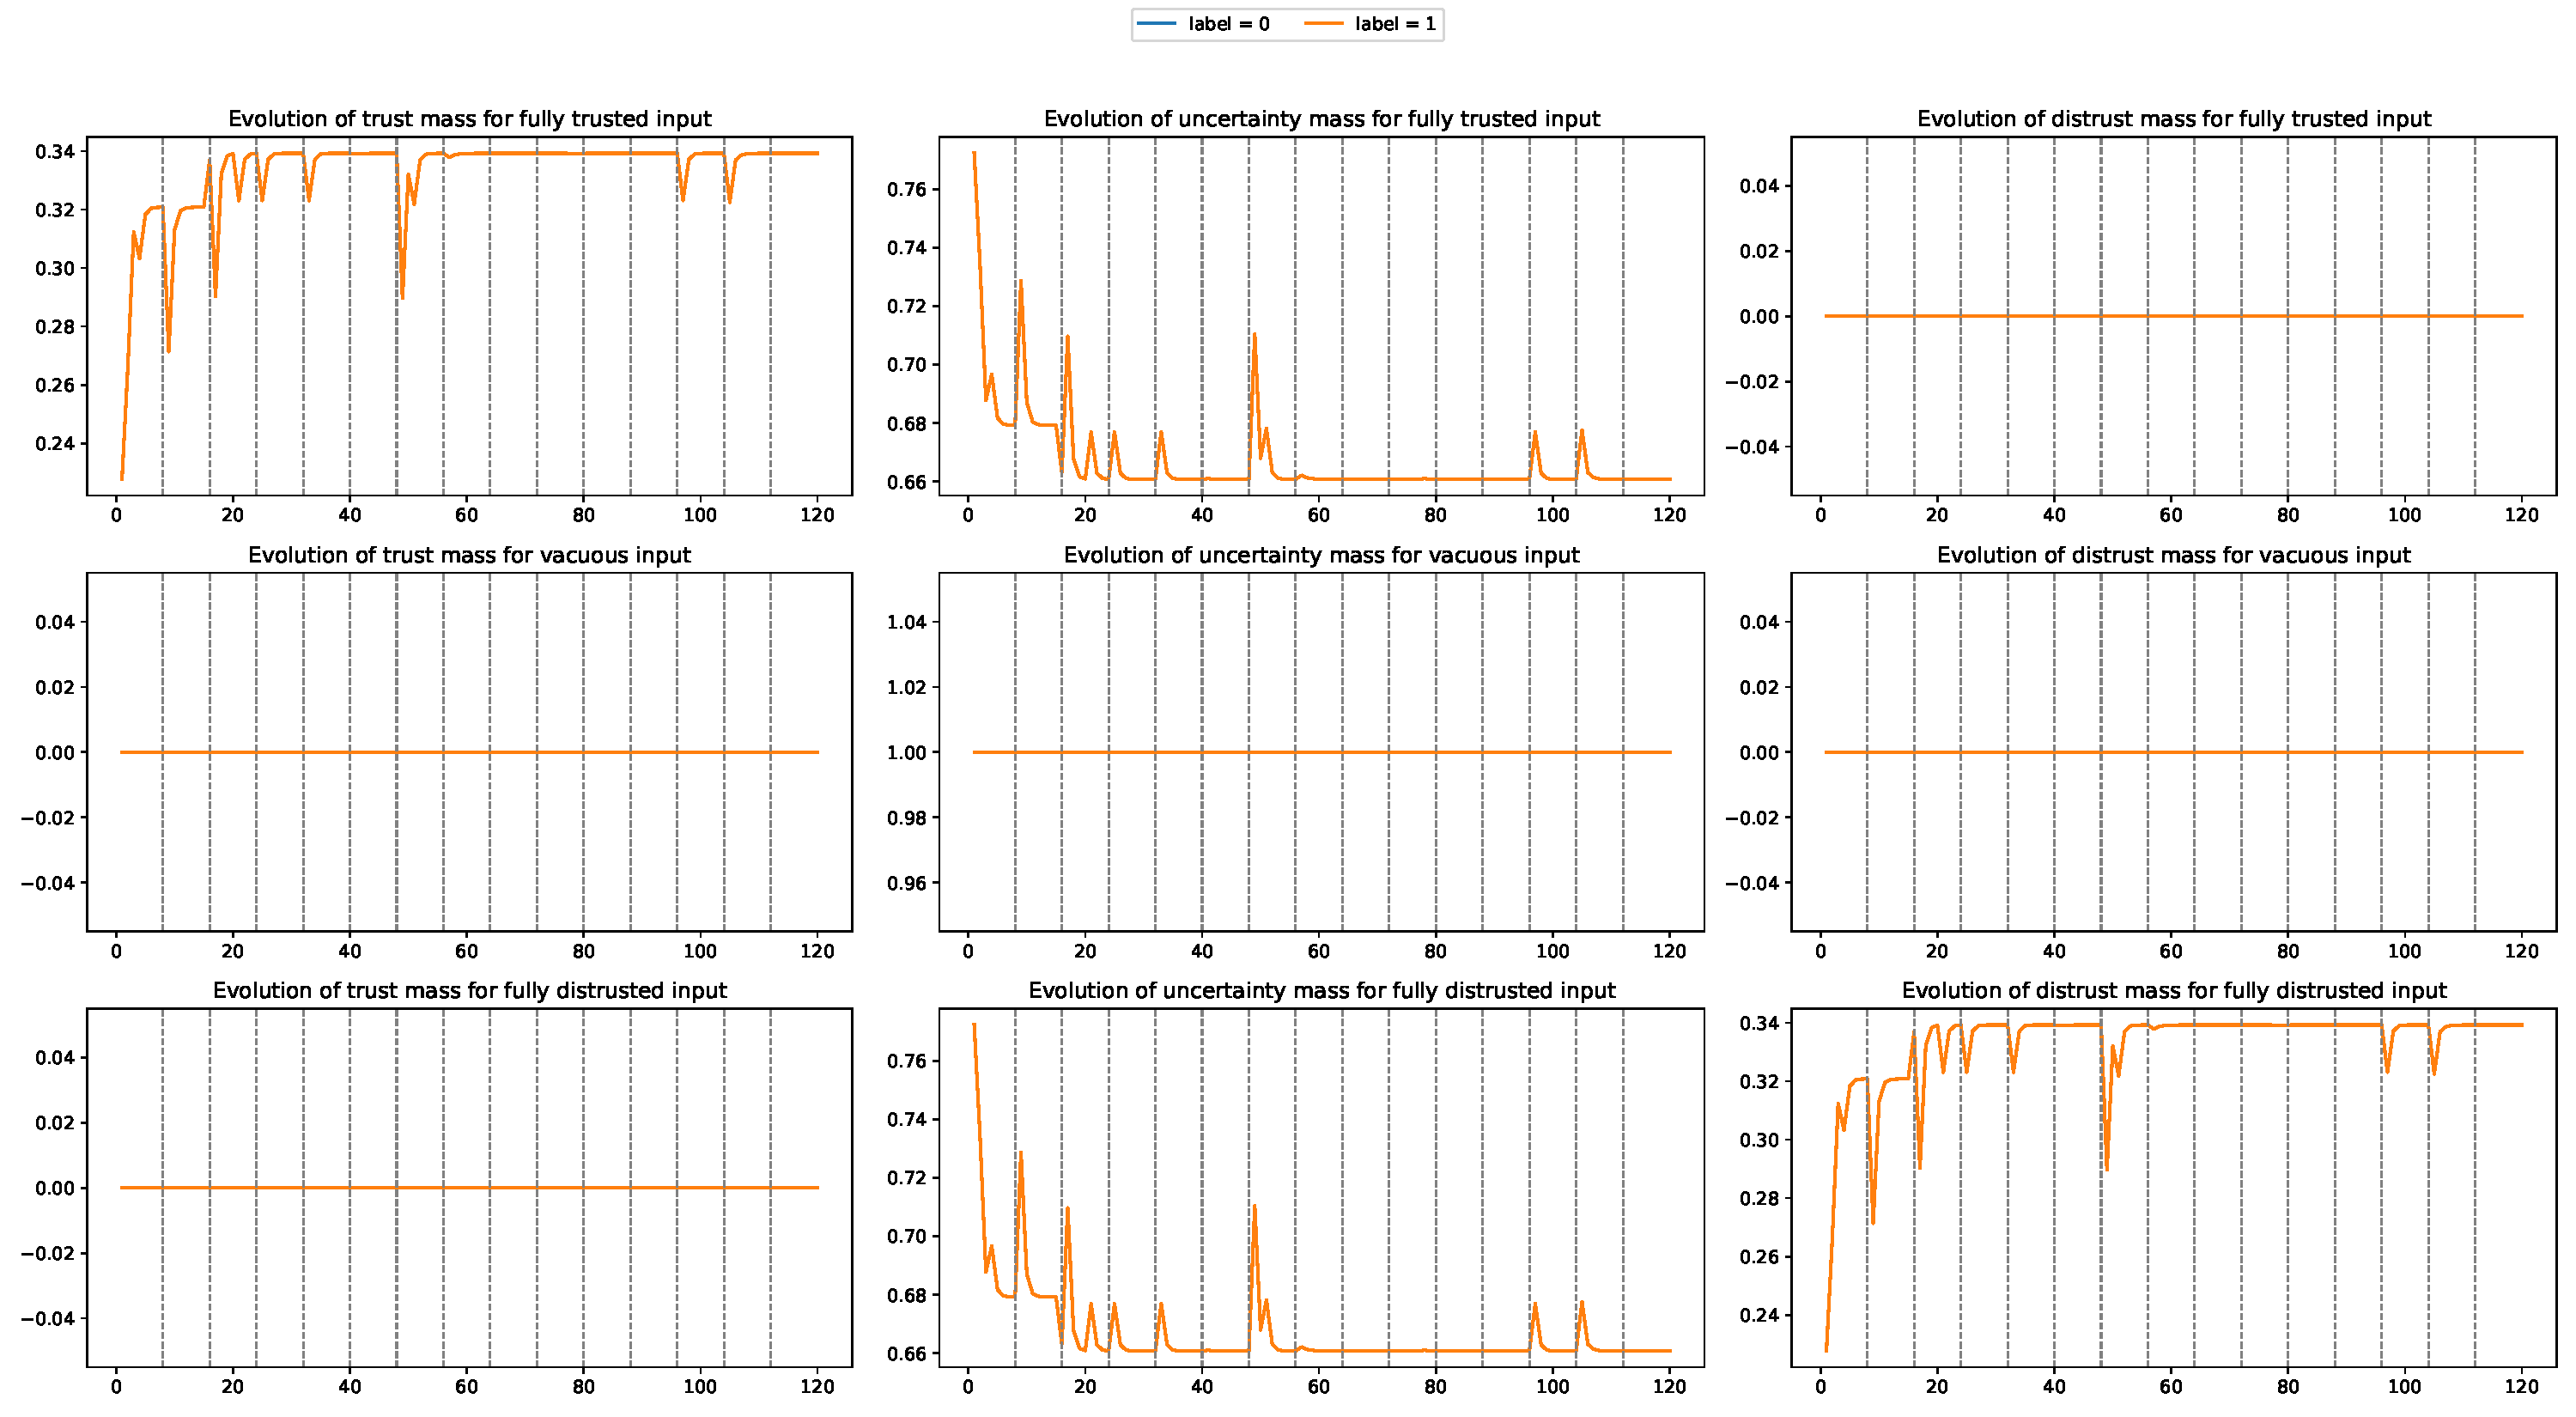
\includegraphics[width=\textwidth]{plots_v2/Cancer/eps=0.1/plot_ptas-v-t.pdf}
  \caption{Features vacuous and labels trusted}
\end{figure}
\begin{figure}[H]
  \includegraphics[width=\textwidth]{plots_v2/Cancer/eps=0.1/plot_ptas-t-d.pdf}
  \caption{Features trusted and labels distrusted}
\end{figure}
\begin{figure}[H]
  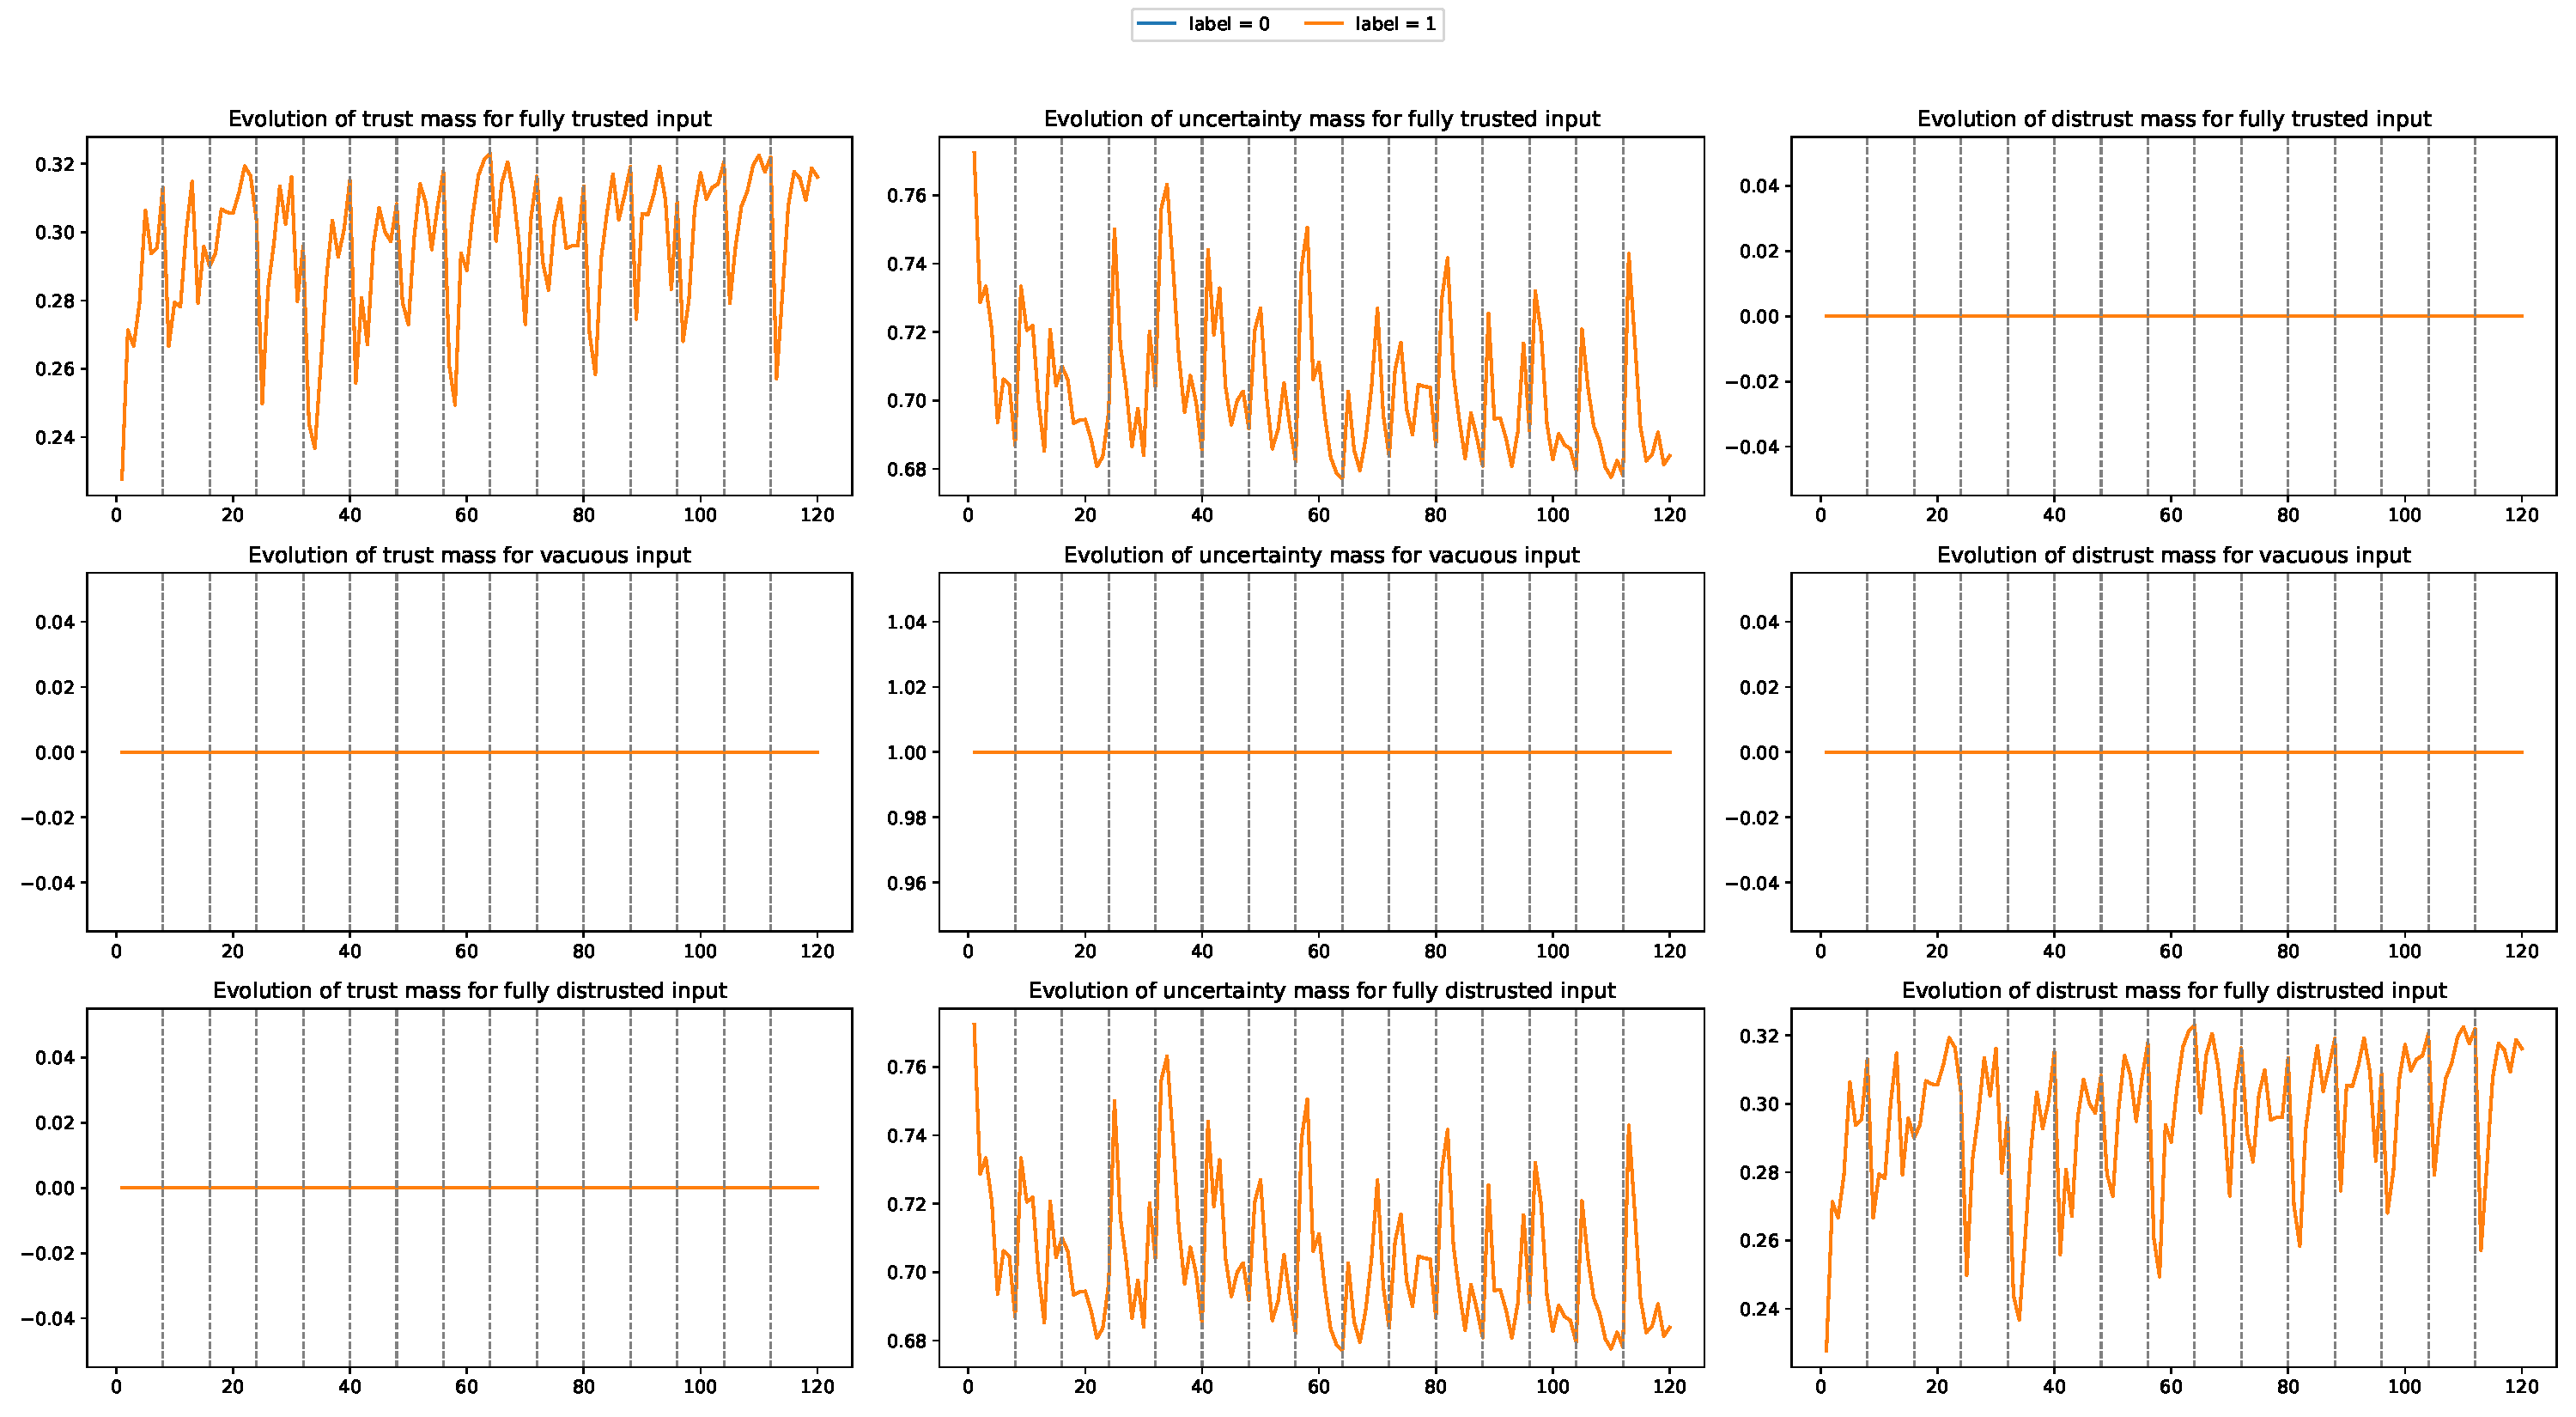
\includegraphics[width=\textwidth]{plots_v2/Cancer/eps=0.1/plot_ptas-t-v.pdf}
  \caption{Features trusted and labels vacuous}
\end{figure}
\begin{figure}[H]
  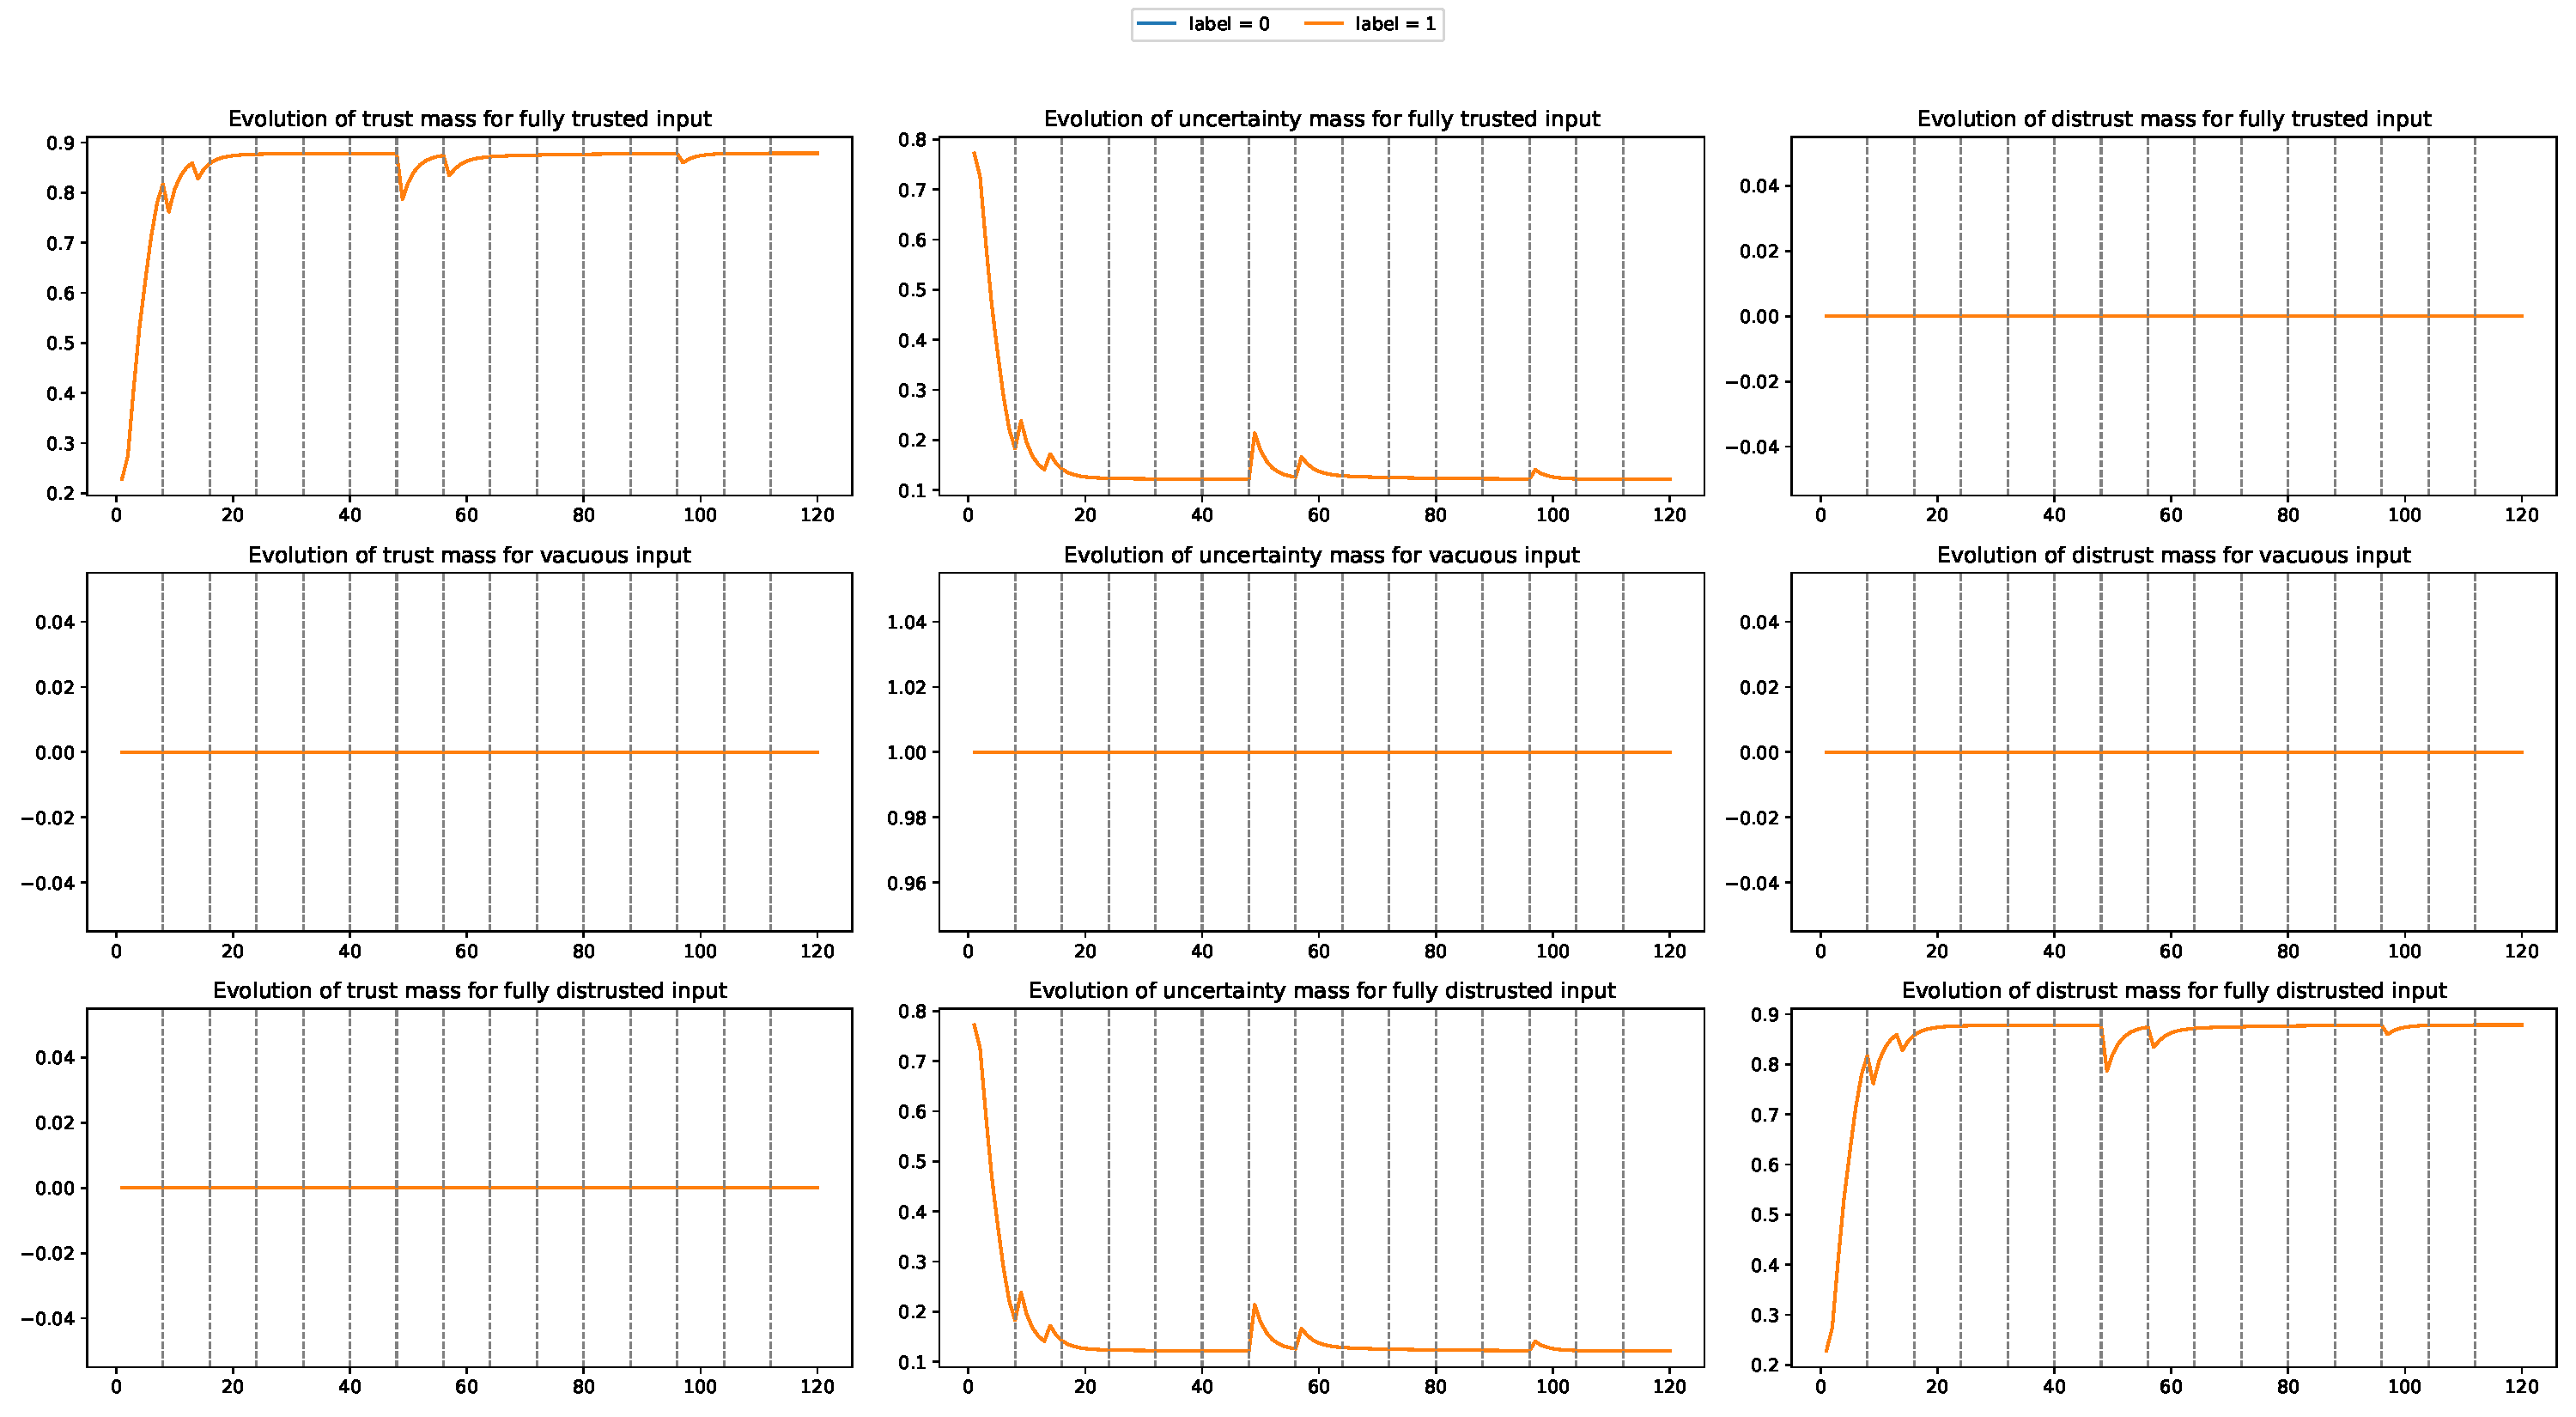
\includegraphics[width=\textwidth]{plots_v2/Cancer/eps=0.1/plot_ptas-t-t.pdf}
  \caption{Features trusted and labels trusted}
\end{figure}

\subsection{Accuracy Evolution for the Cancer Model (\cref{exp:1})}\label{sec:resmnistaccapp}
\begin{figure}[H]
\centering
\begin{subfigure}[b]{0.32\textwidth}
  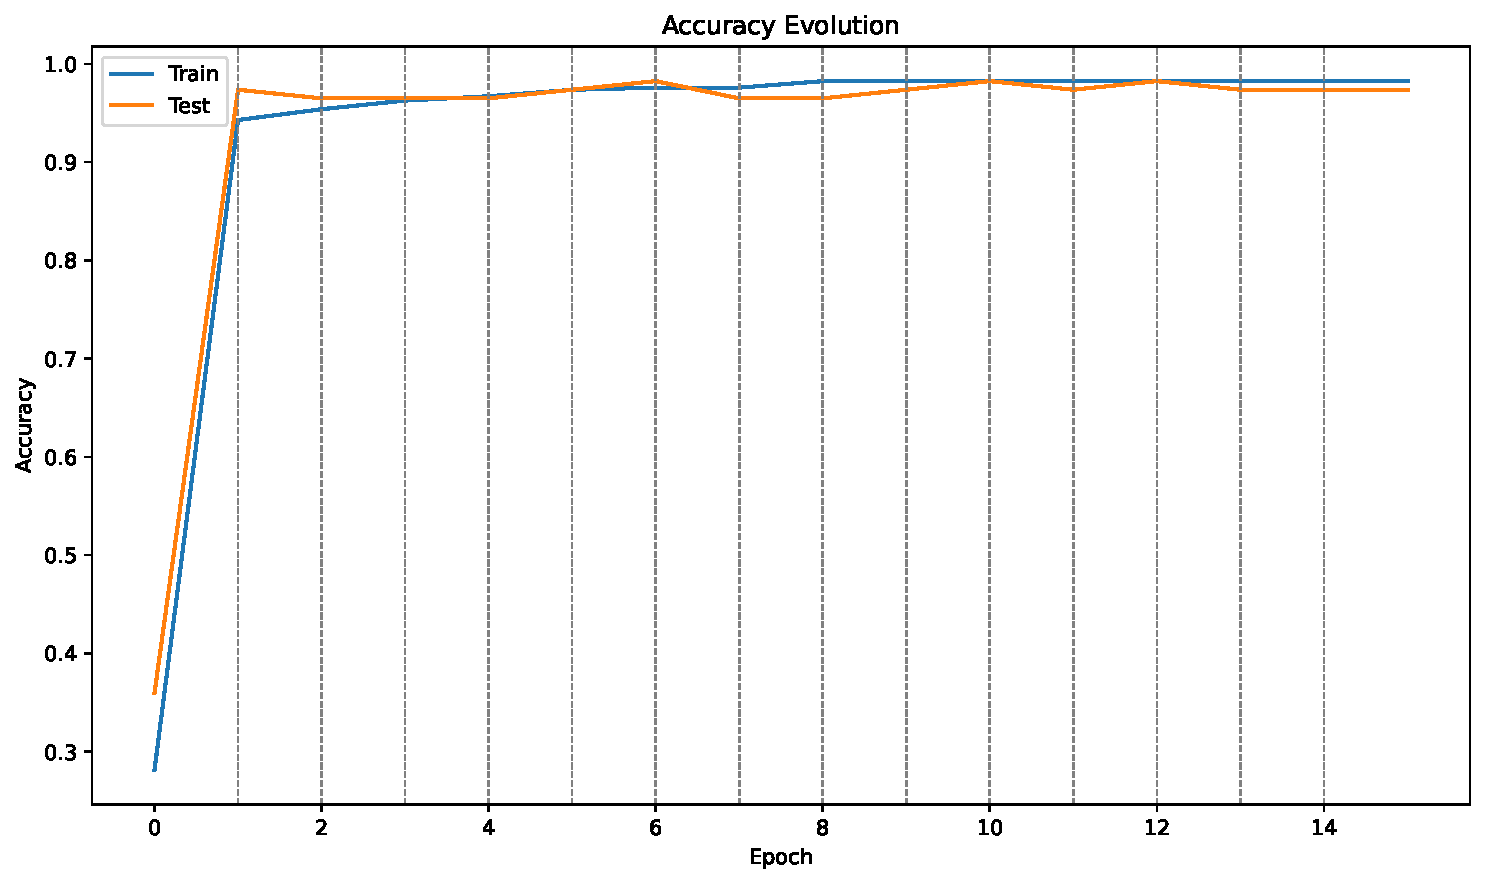
\includegraphics[width=\textwidth]{plots_v2/Cancer/eps=0.1/accuracy_evolution-t-t.pdf}
  \caption{Clean Features and Labels}
\end{subfigure}
\begin{subfigure}[b]{0.32\textwidth}
  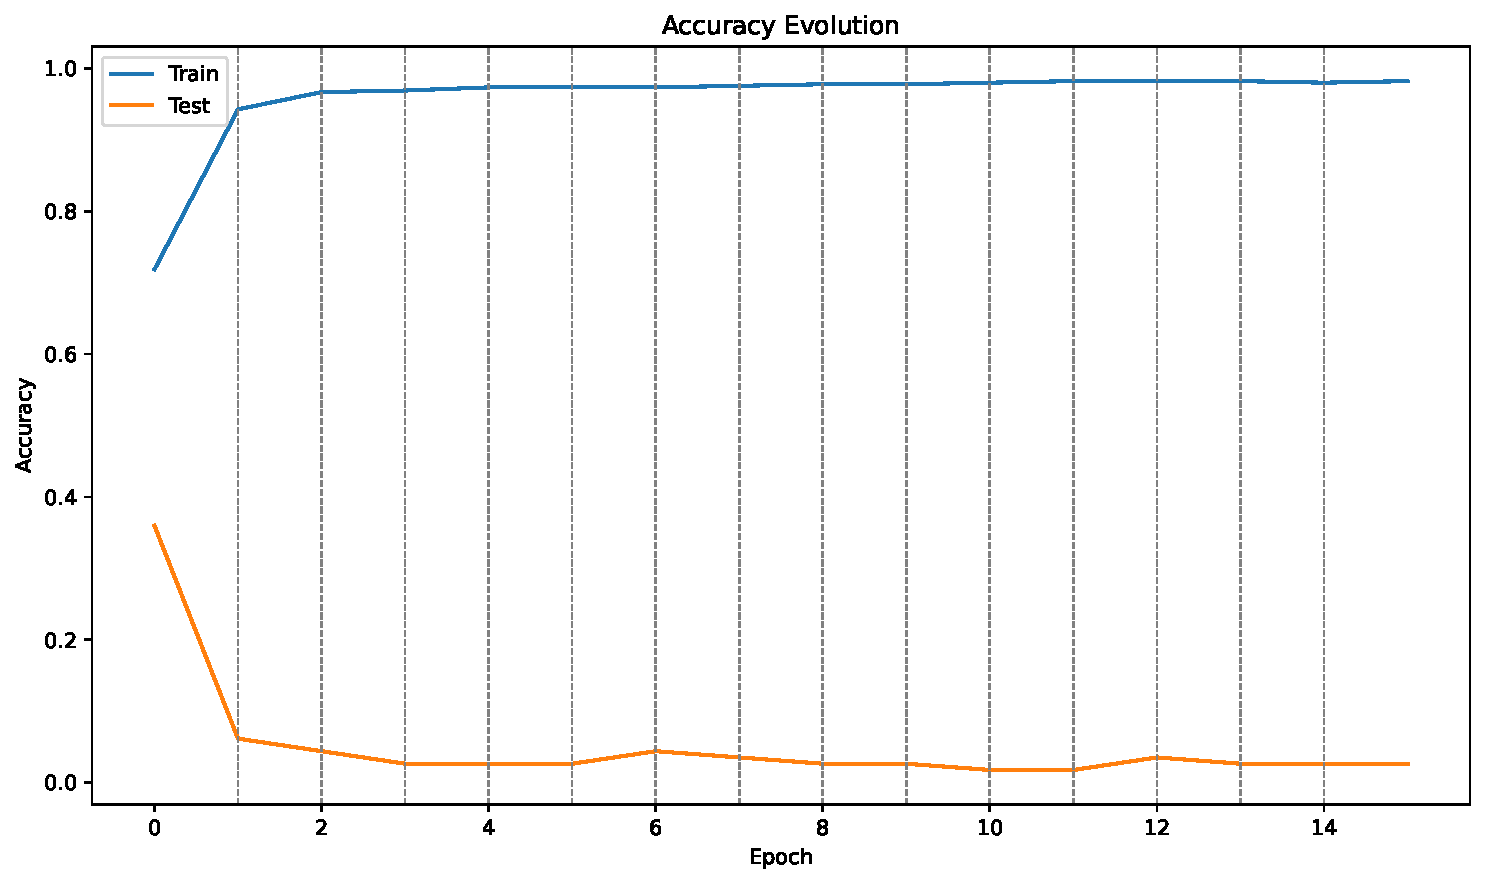
\includegraphics[width=\textwidth]{plots_v2/Cancer/eps=0.1/accuracy_evolution-t-d.pdf}
  \caption{Clean Features and Corrupted Labels}
\end{subfigure}
\begin{subfigure}[b]{0.32\textwidth}
  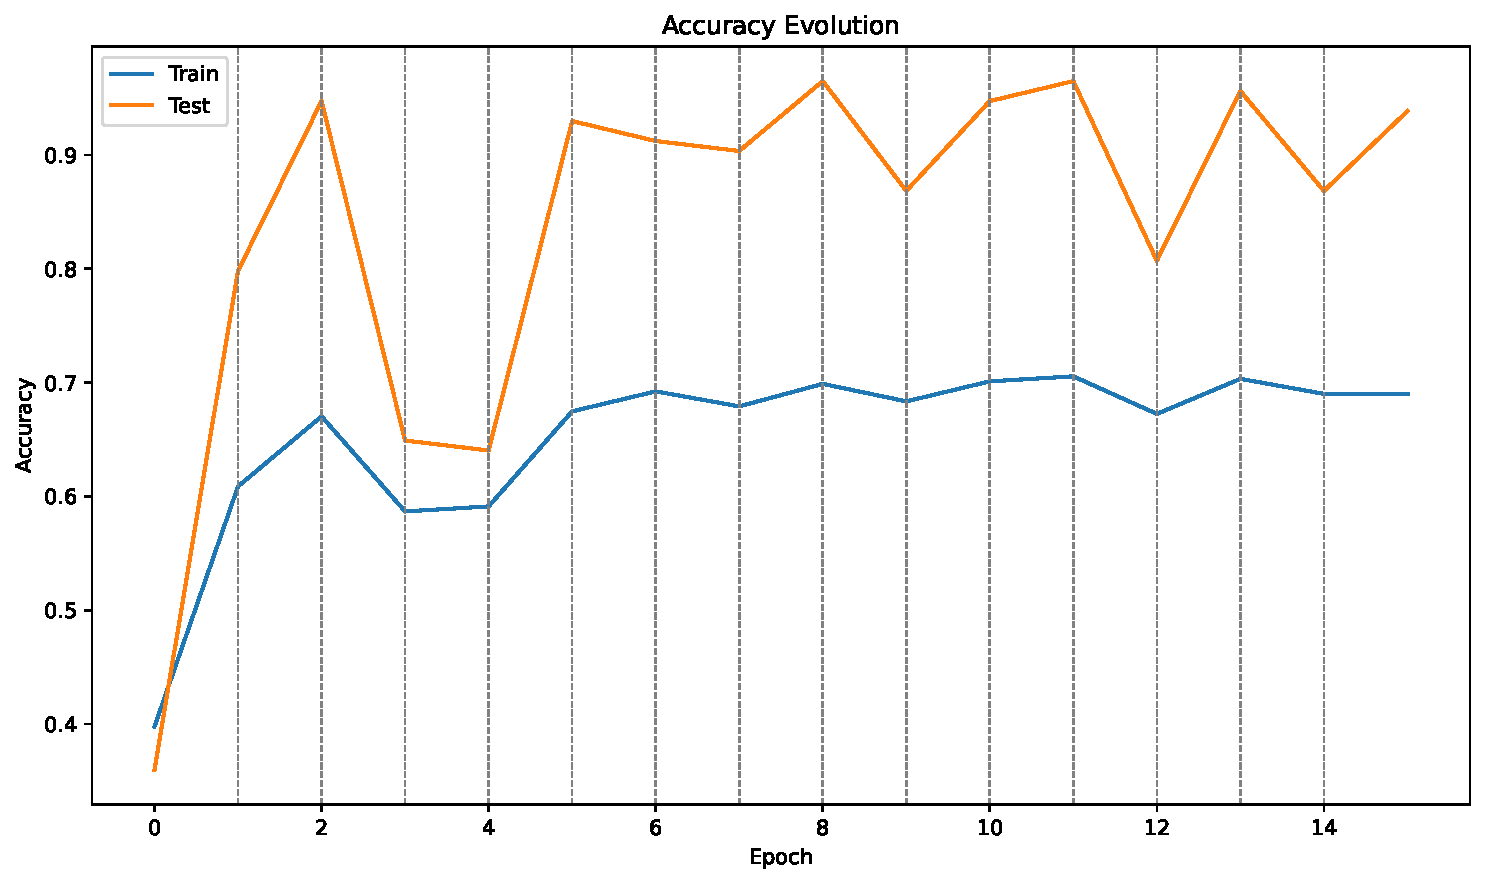
\includegraphics[width=\textwidth]{plots_v2/Cancer/eps=0.1/accuracy_evolution-t-v.pdf}
  \caption{Clean Features and Noisy Labels}
\end{subfigure}
\begin{subfigure}[b]{0.32\textwidth}
  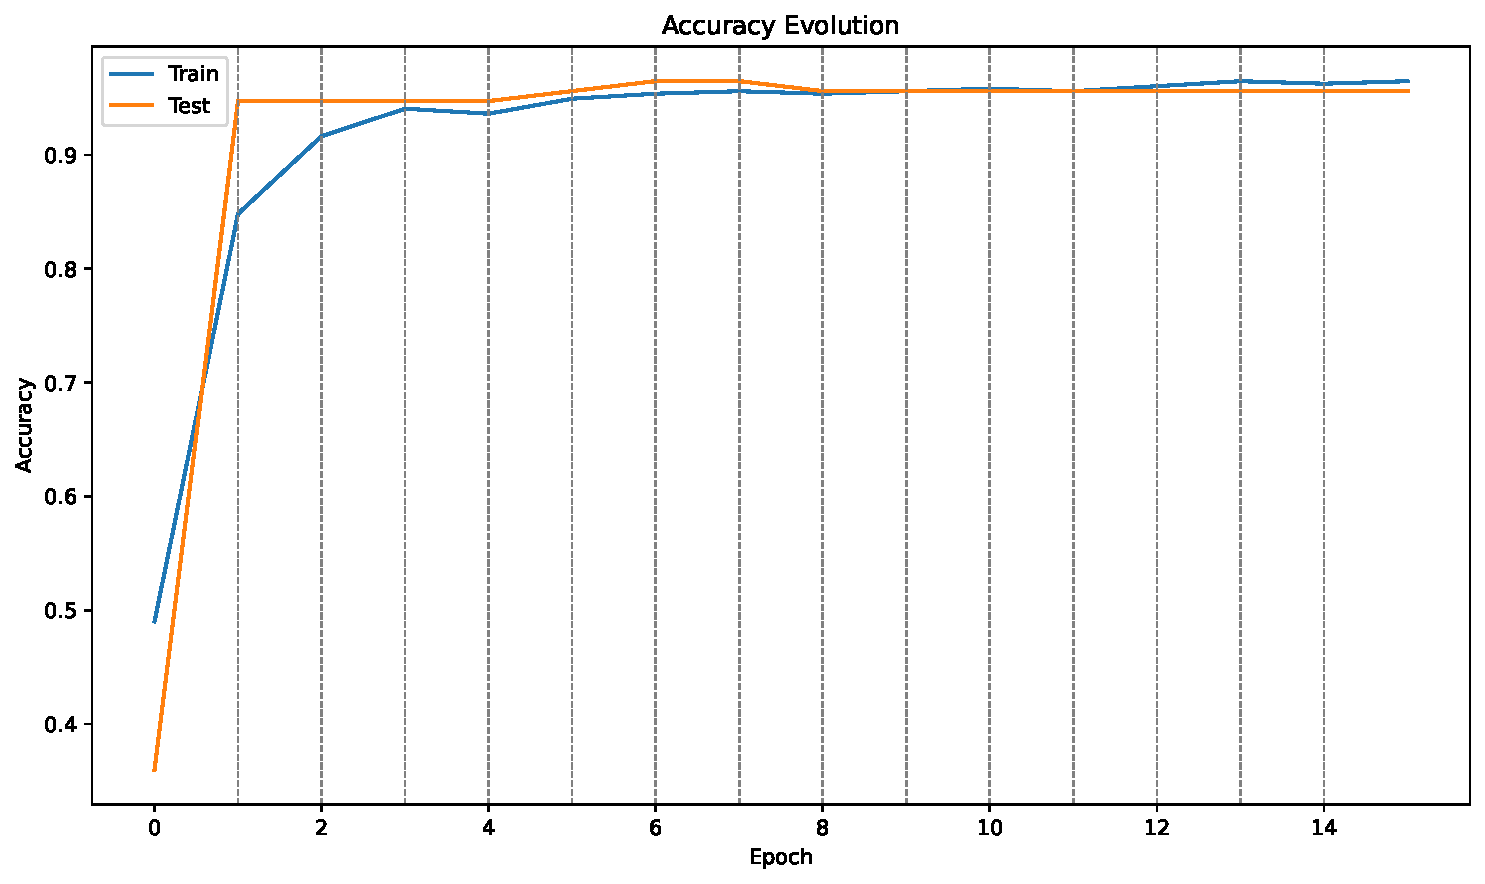
\includegraphics[width=\textwidth]{plots_v2/Cancer/eps=0.1/accuracy_evolution-v-t.pdf}
  \caption{Noisy Features and Clean Labels}
\end{subfigure}
\begin{subfigure}[b]{0.32\textwidth}
  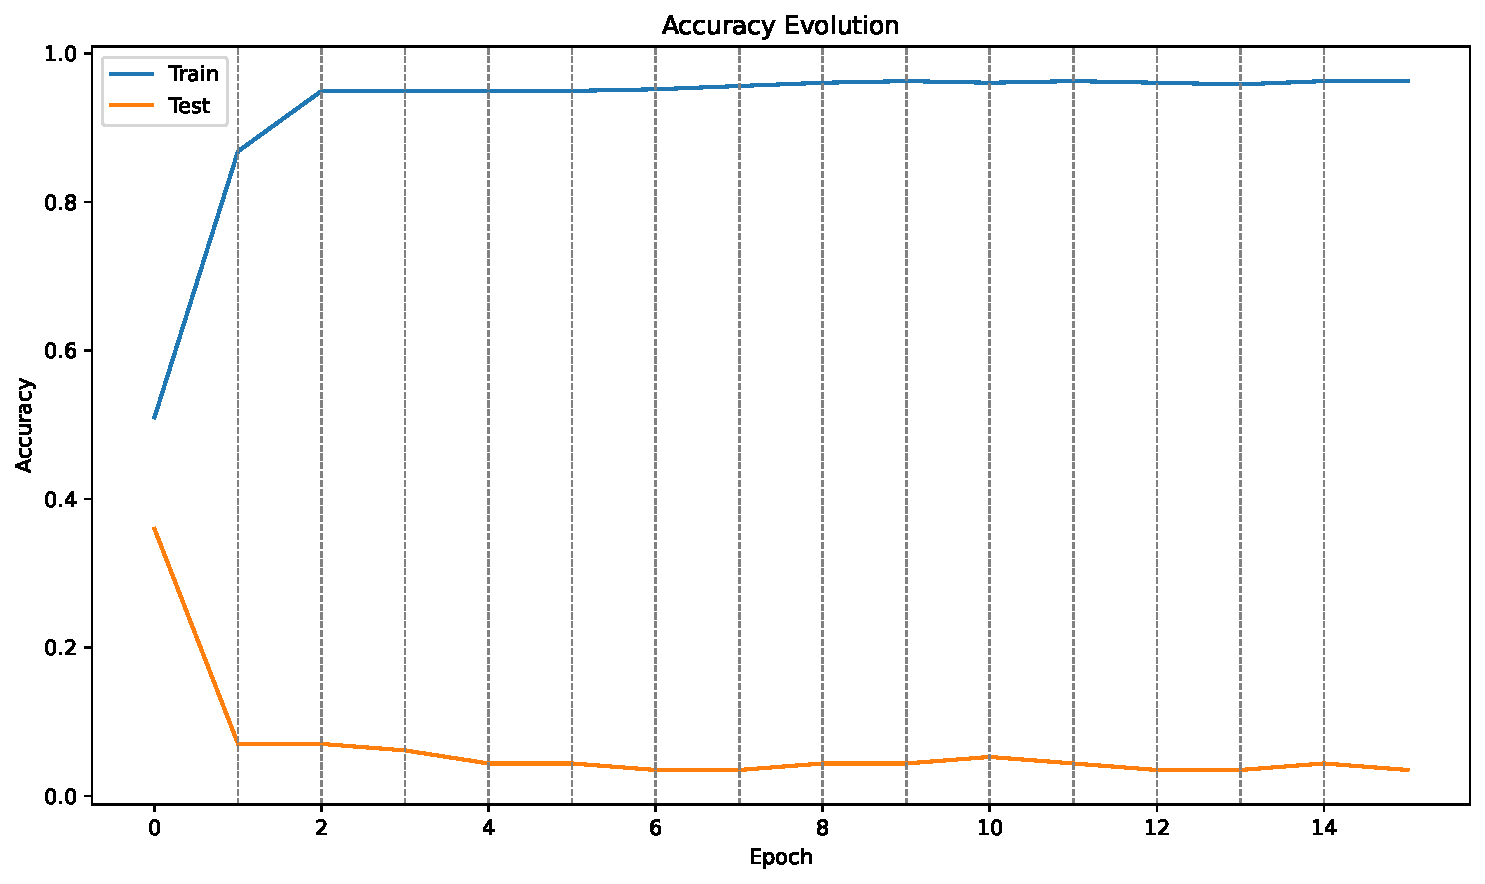
\includegraphics[width=\textwidth]{plots_v2/Cancer/eps=0.1/accuracy_evolution-v-d.pdf}
  \caption{Noisy Features and Corrupted Labels}
\end{subfigure}
\begin{subfigure}[b]{0.32\textwidth}
  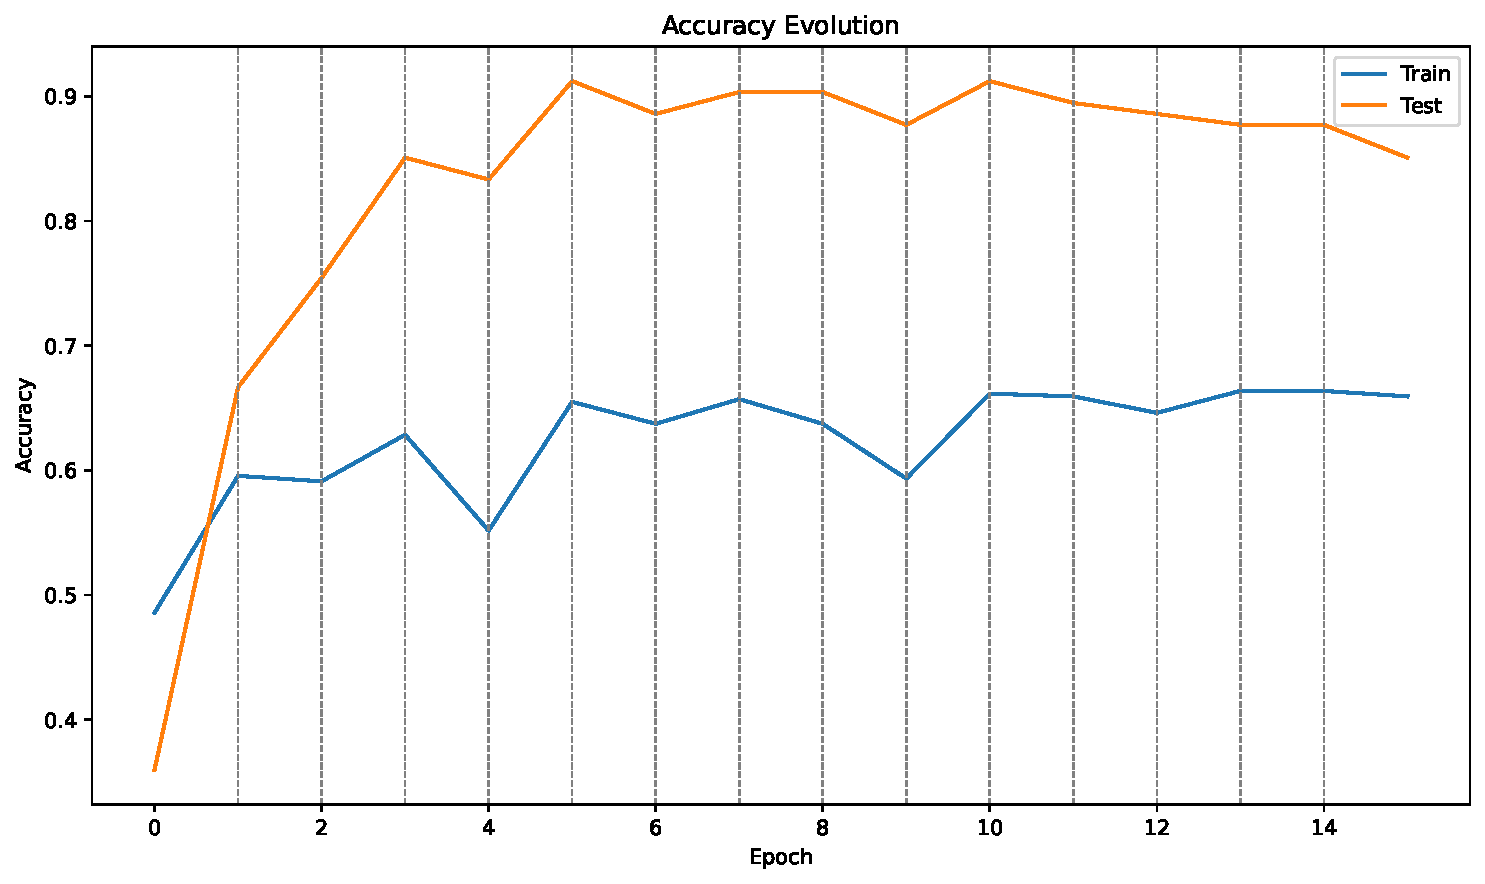
\includegraphics[width=\textwidth]{plots_v2/Cancer/eps=0.1/accuracy_evolution-v-v.pdf}
  \caption{Noisy Features and Noisy Labels}
\end{subfigure}
\begin{subfigure}[b]{0.32\textwidth}
  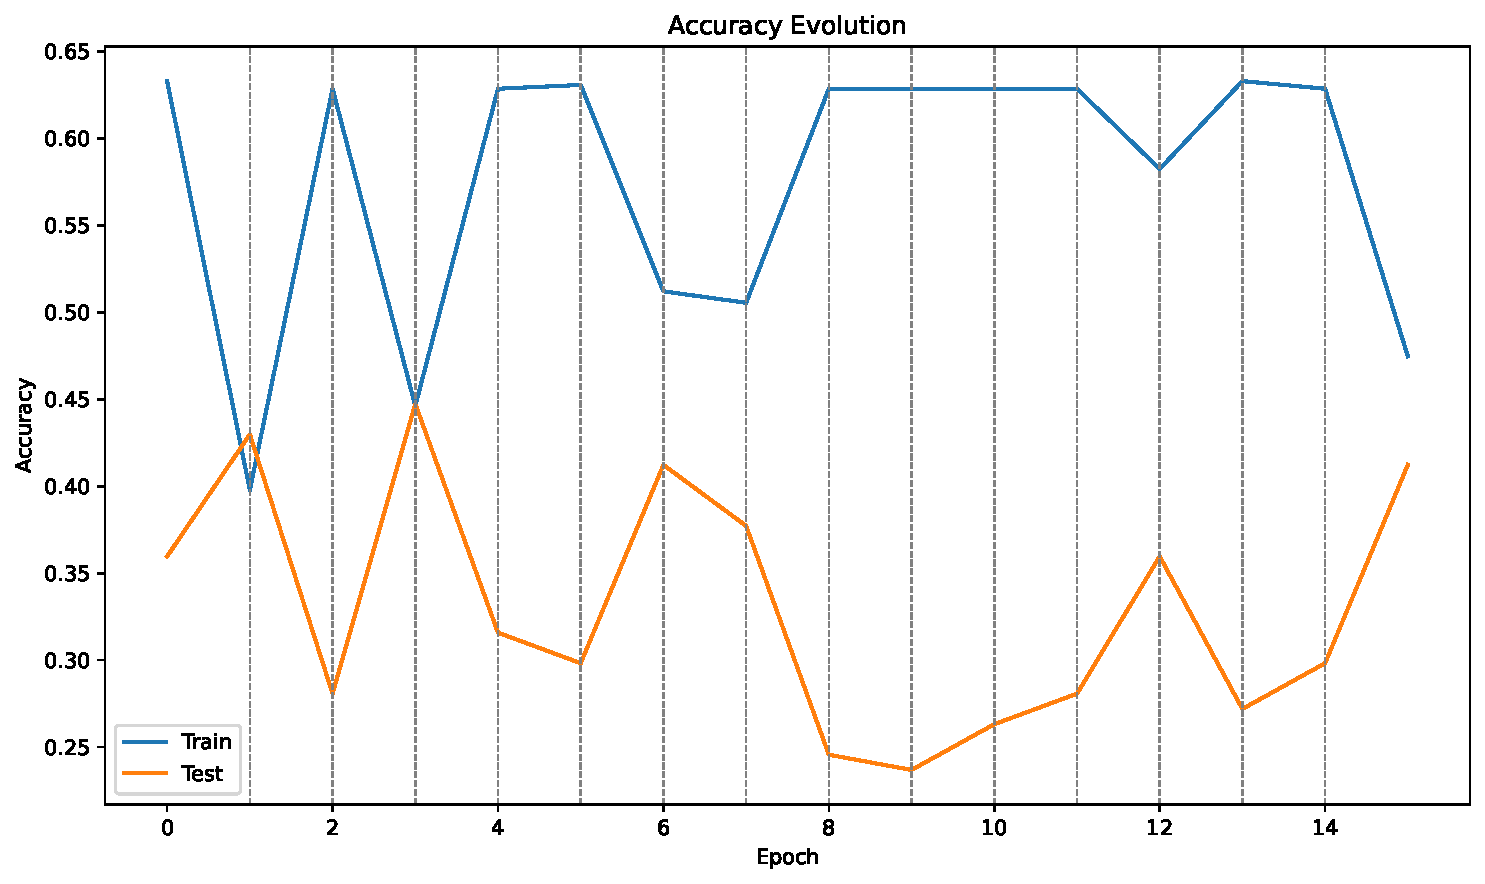
\includegraphics[width=\textwidth]{plots_v2/Cancer/eps=0.1/accuracy_evolution-d-t.pdf}
  \caption{Corrupted Features and Clean Labels}
\end{subfigure}
\begin{subfigure}[b]{0.32\textwidth}
  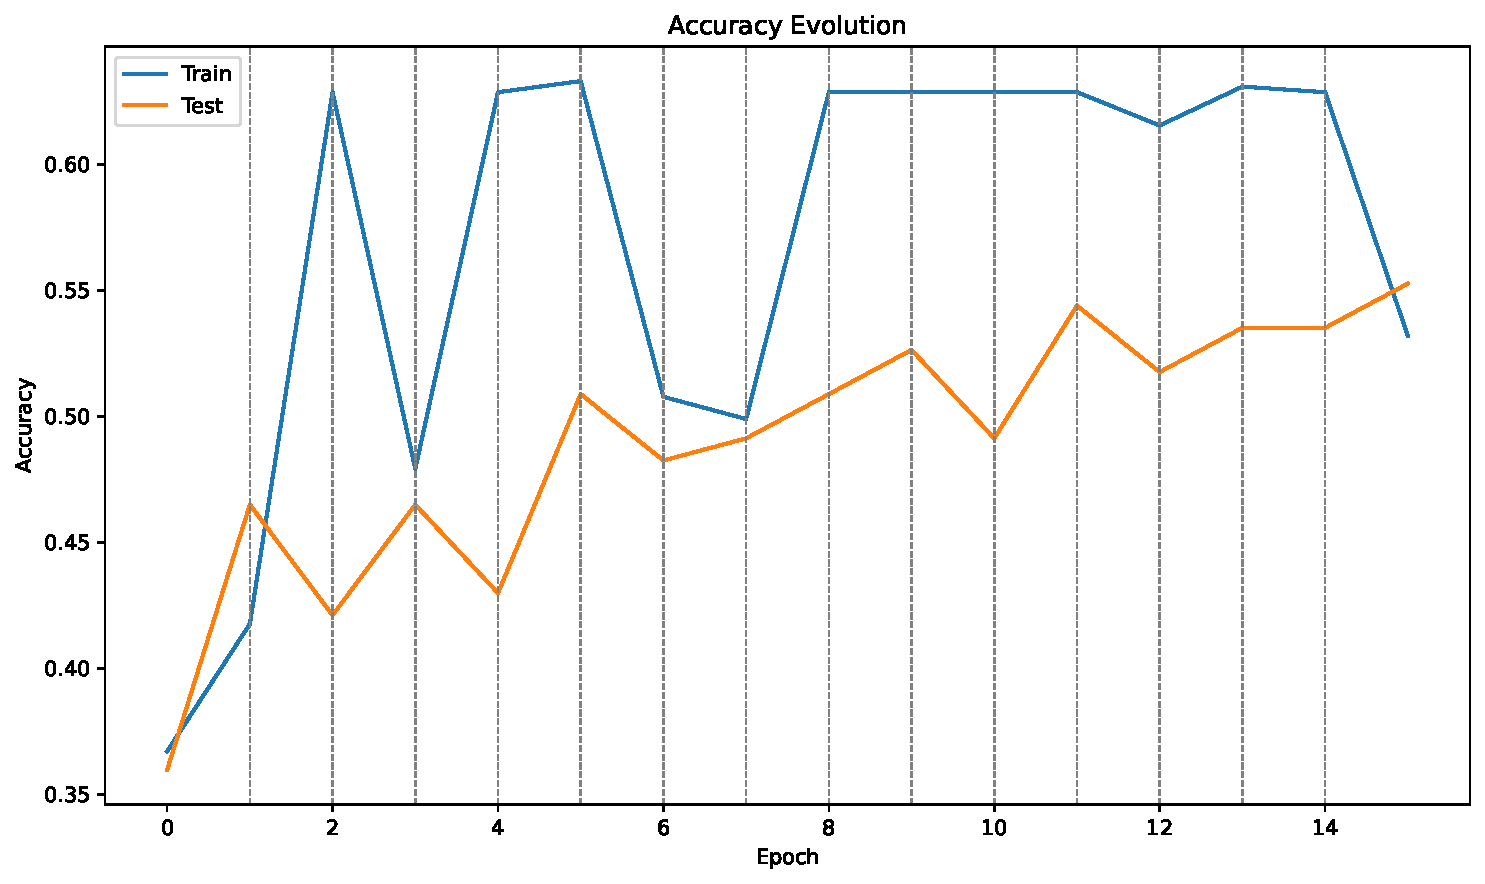
\includegraphics[width=\textwidth]{plots_v2/Cancer/eps=0.1/accuracy_evolution-d-d.pdf}
  \caption{Corrupted Features and Corrupted Labels}
\end{subfigure}
\begin{subfigure}[b]{0.32\textwidth}
  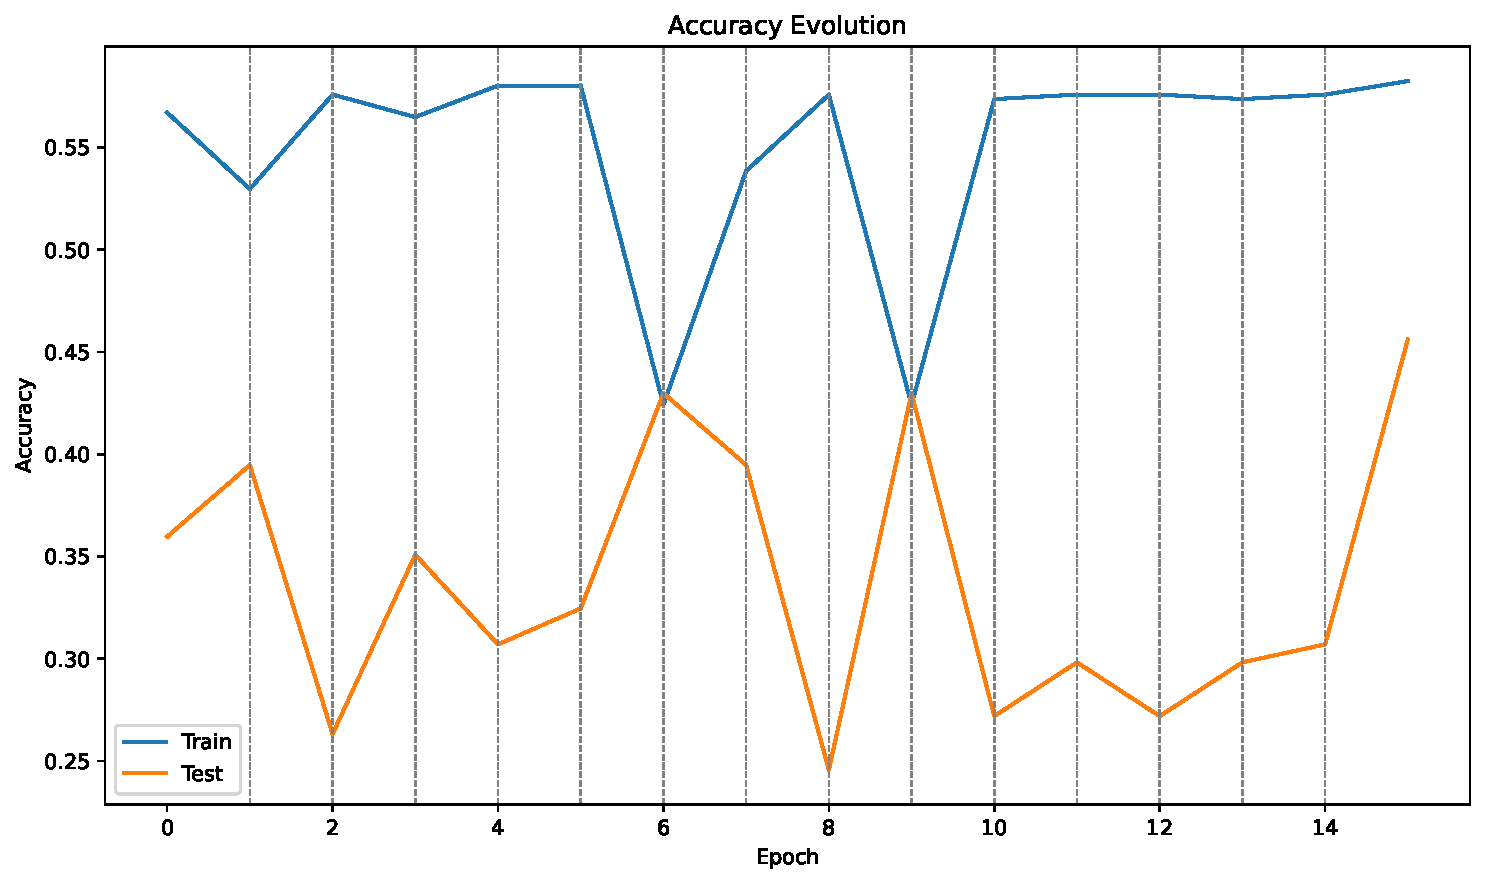
\includegraphics[width=\textwidth]{plots_v2/Cancer/eps=0.1/accuracy_evolution-d-v.pdf}
  \caption{Corrupted Features and Noisy Labels}
\end{subfigure}
\caption{Accuracy evolution of the Cancer model under different combinations of clean, corrupted, and noisy features and labels.}
\label{fig:Acccancer}
\end{figure}
% \begin{figure}[H]
%     \centering
%     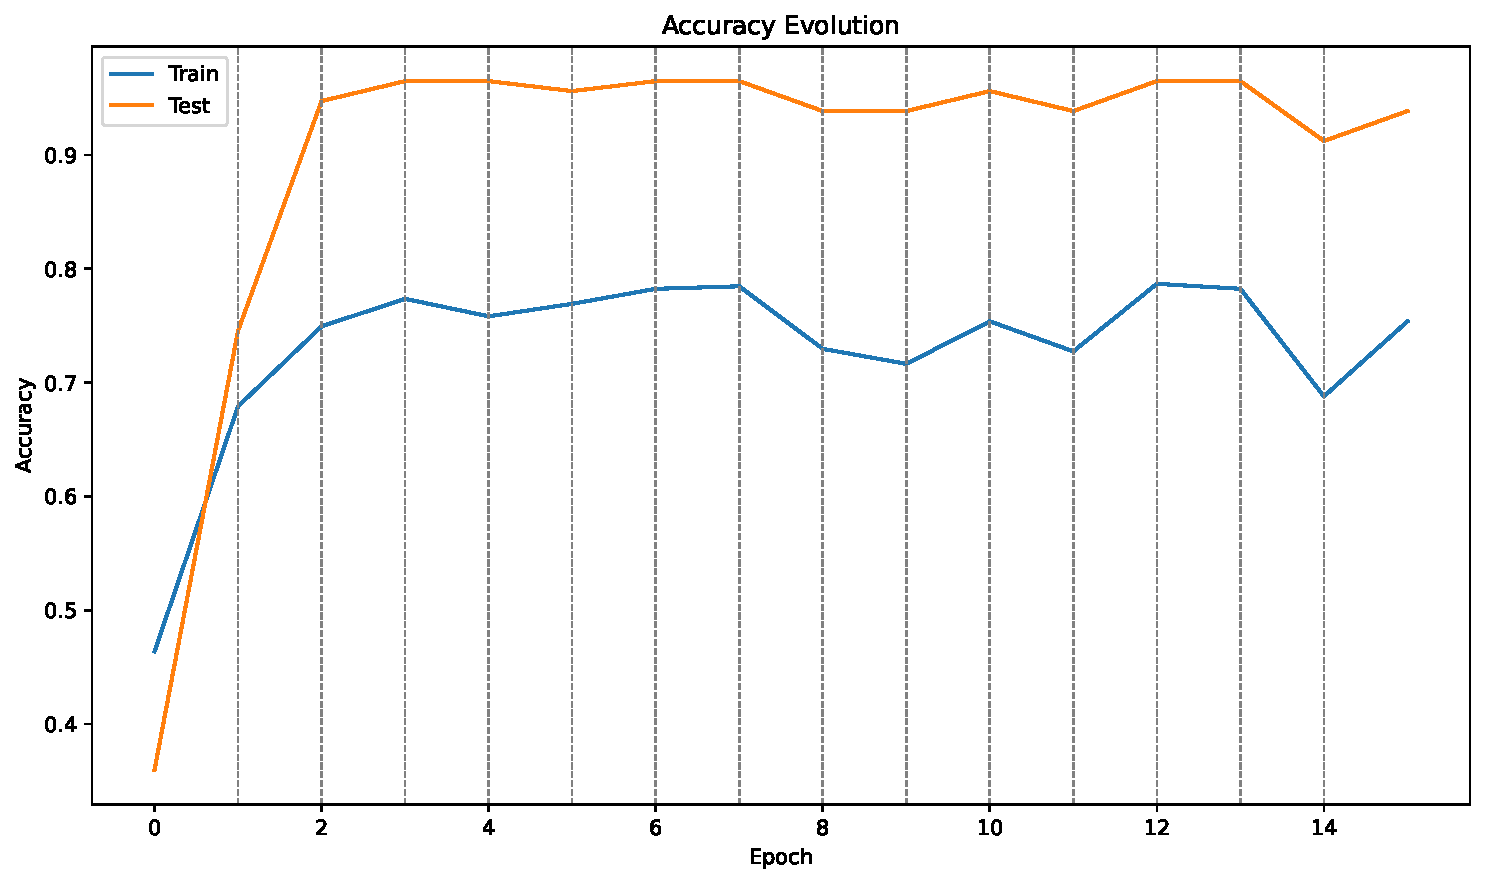
\includegraphics[width=0.8\linewidth]{good_plots/accuracy/Cancer/0.15-0.25/Cancer-noise-noise.pdf}
%     \caption{Accuracy evolution of the Cancer model when reducing the noise for noised features and labels.}
%     \label{fig:AcccancerInt}
% \end{figure}

\subsection{MNIST with Vacuous Trust Assessment (\cref{exp:2})}\label{sec:resmnist}
\begin{figure}[H]
  \centering
  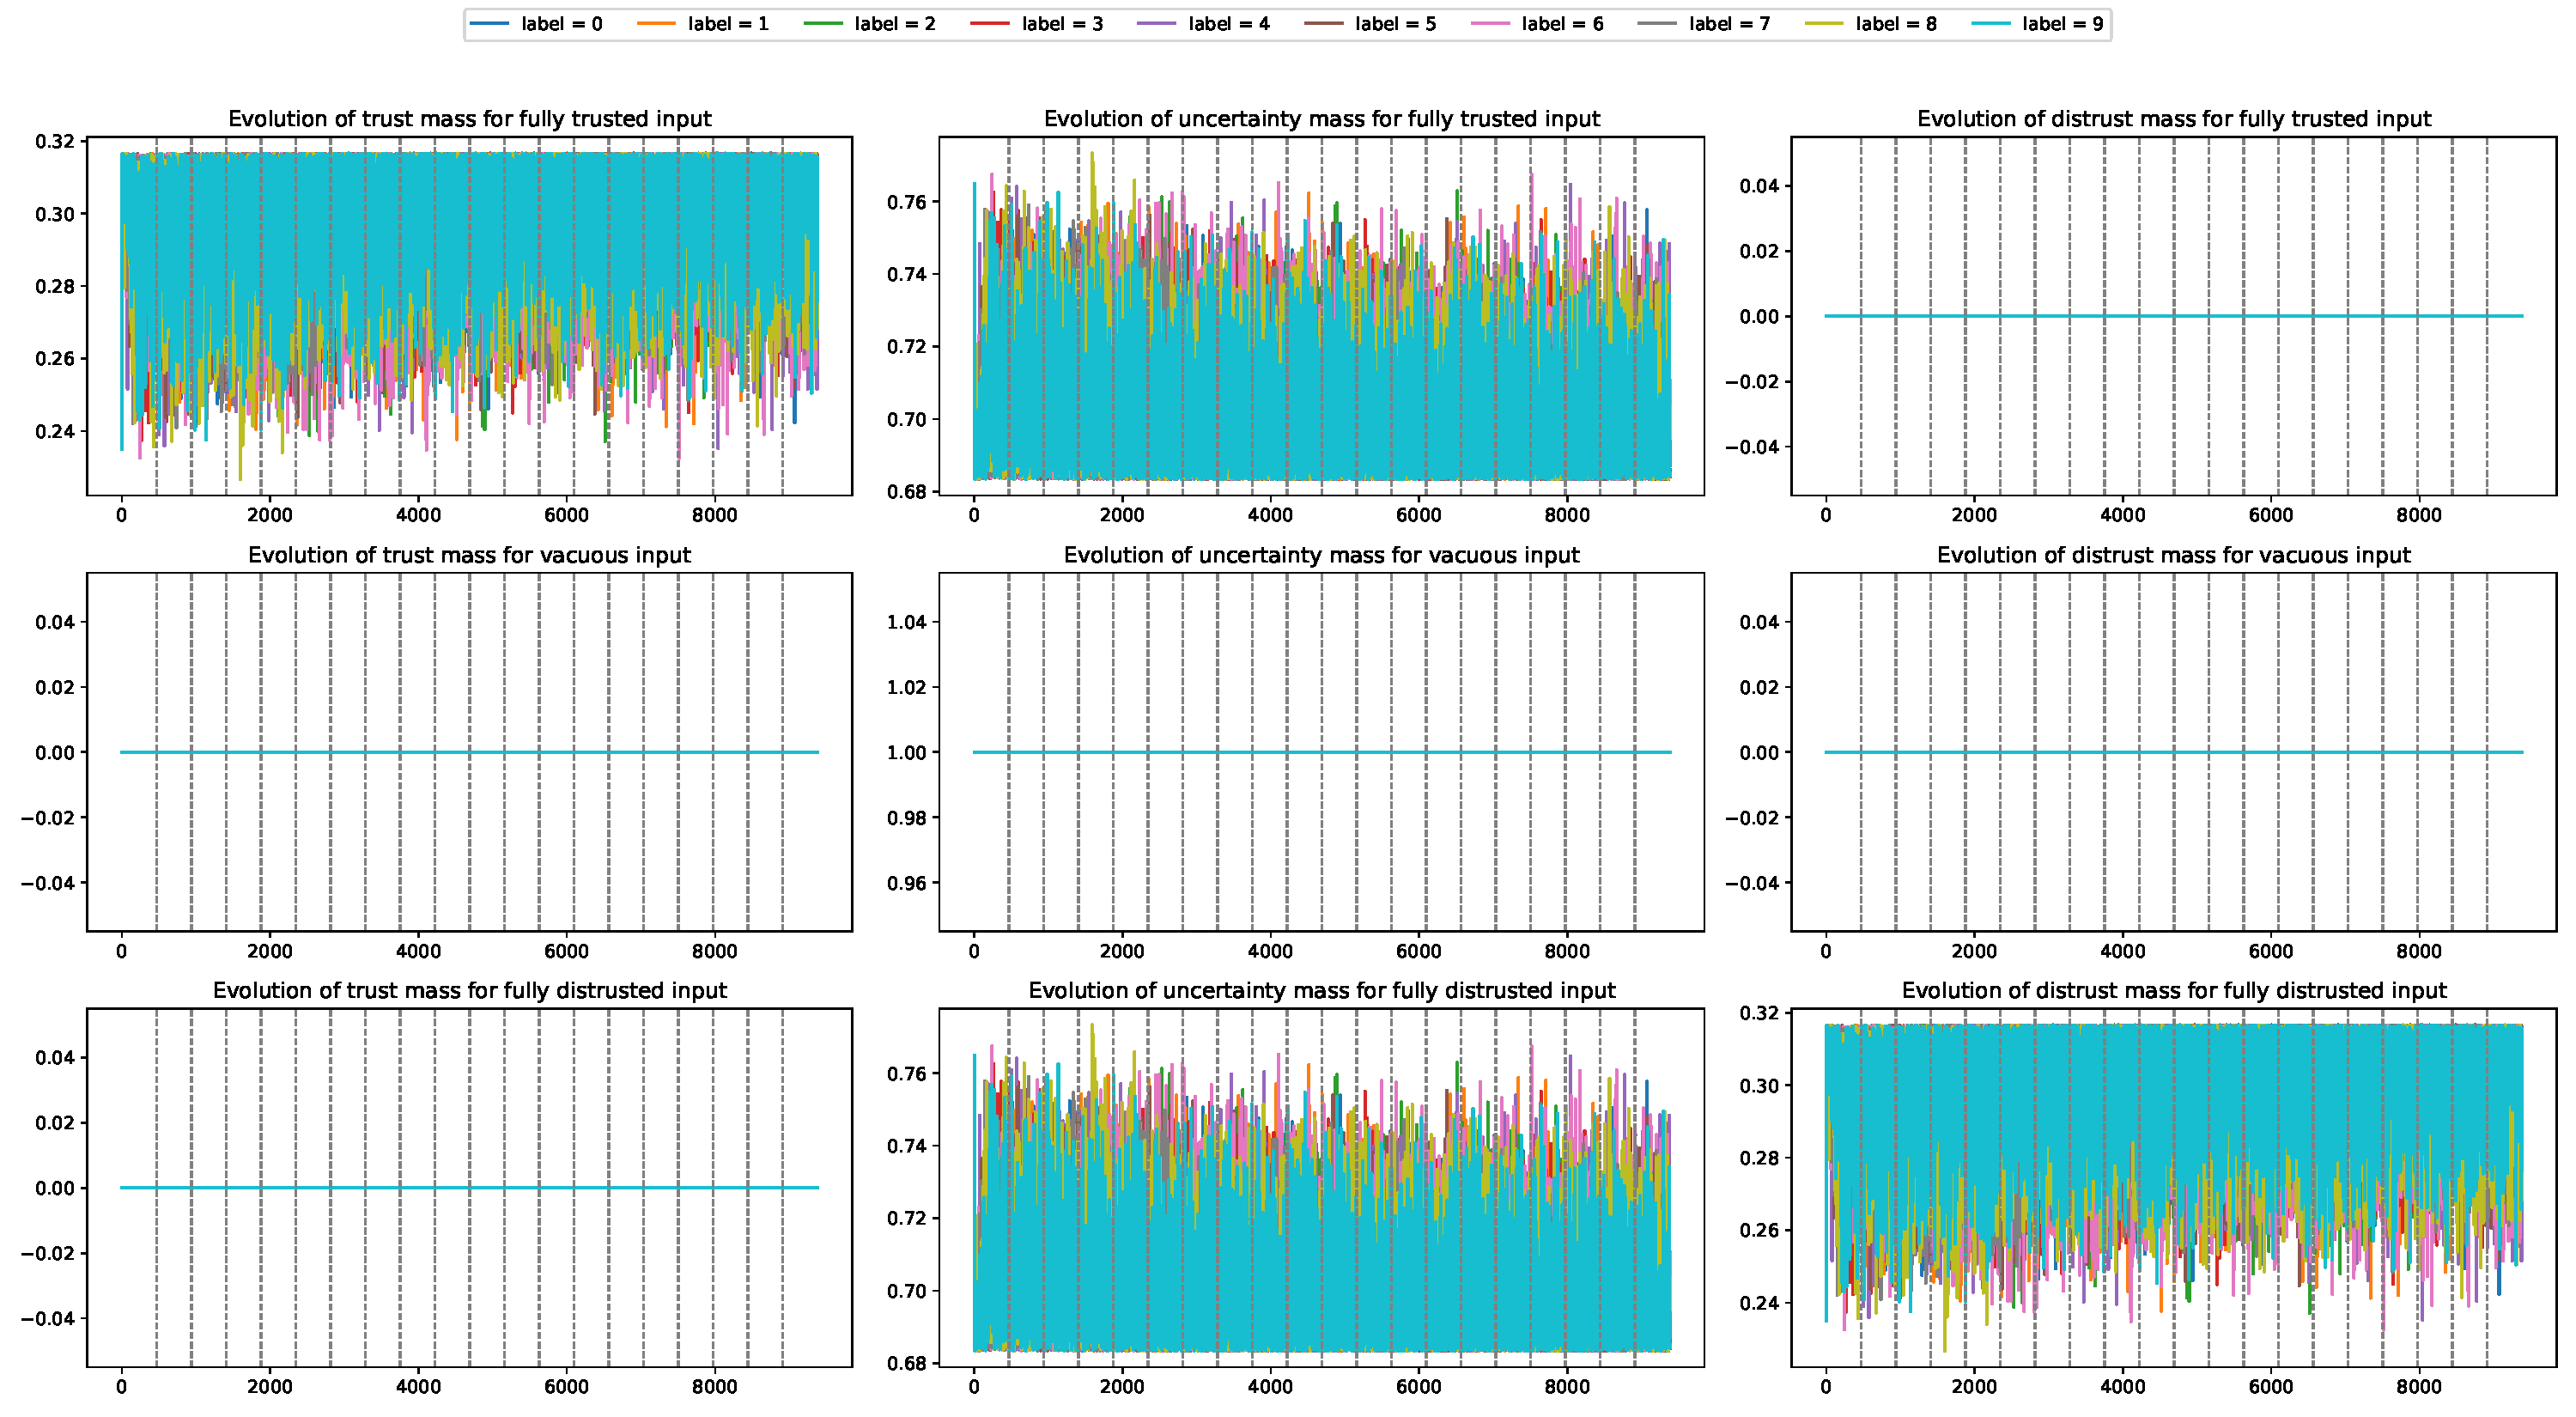
\includegraphics[width=\textwidth]{plots_v2/MNIST/architecture/plot_ptas-16-v-v.pdf}
  \caption{16 Hidden neurons}
\end{figure}
\begin{figure}[H]
  \centering
  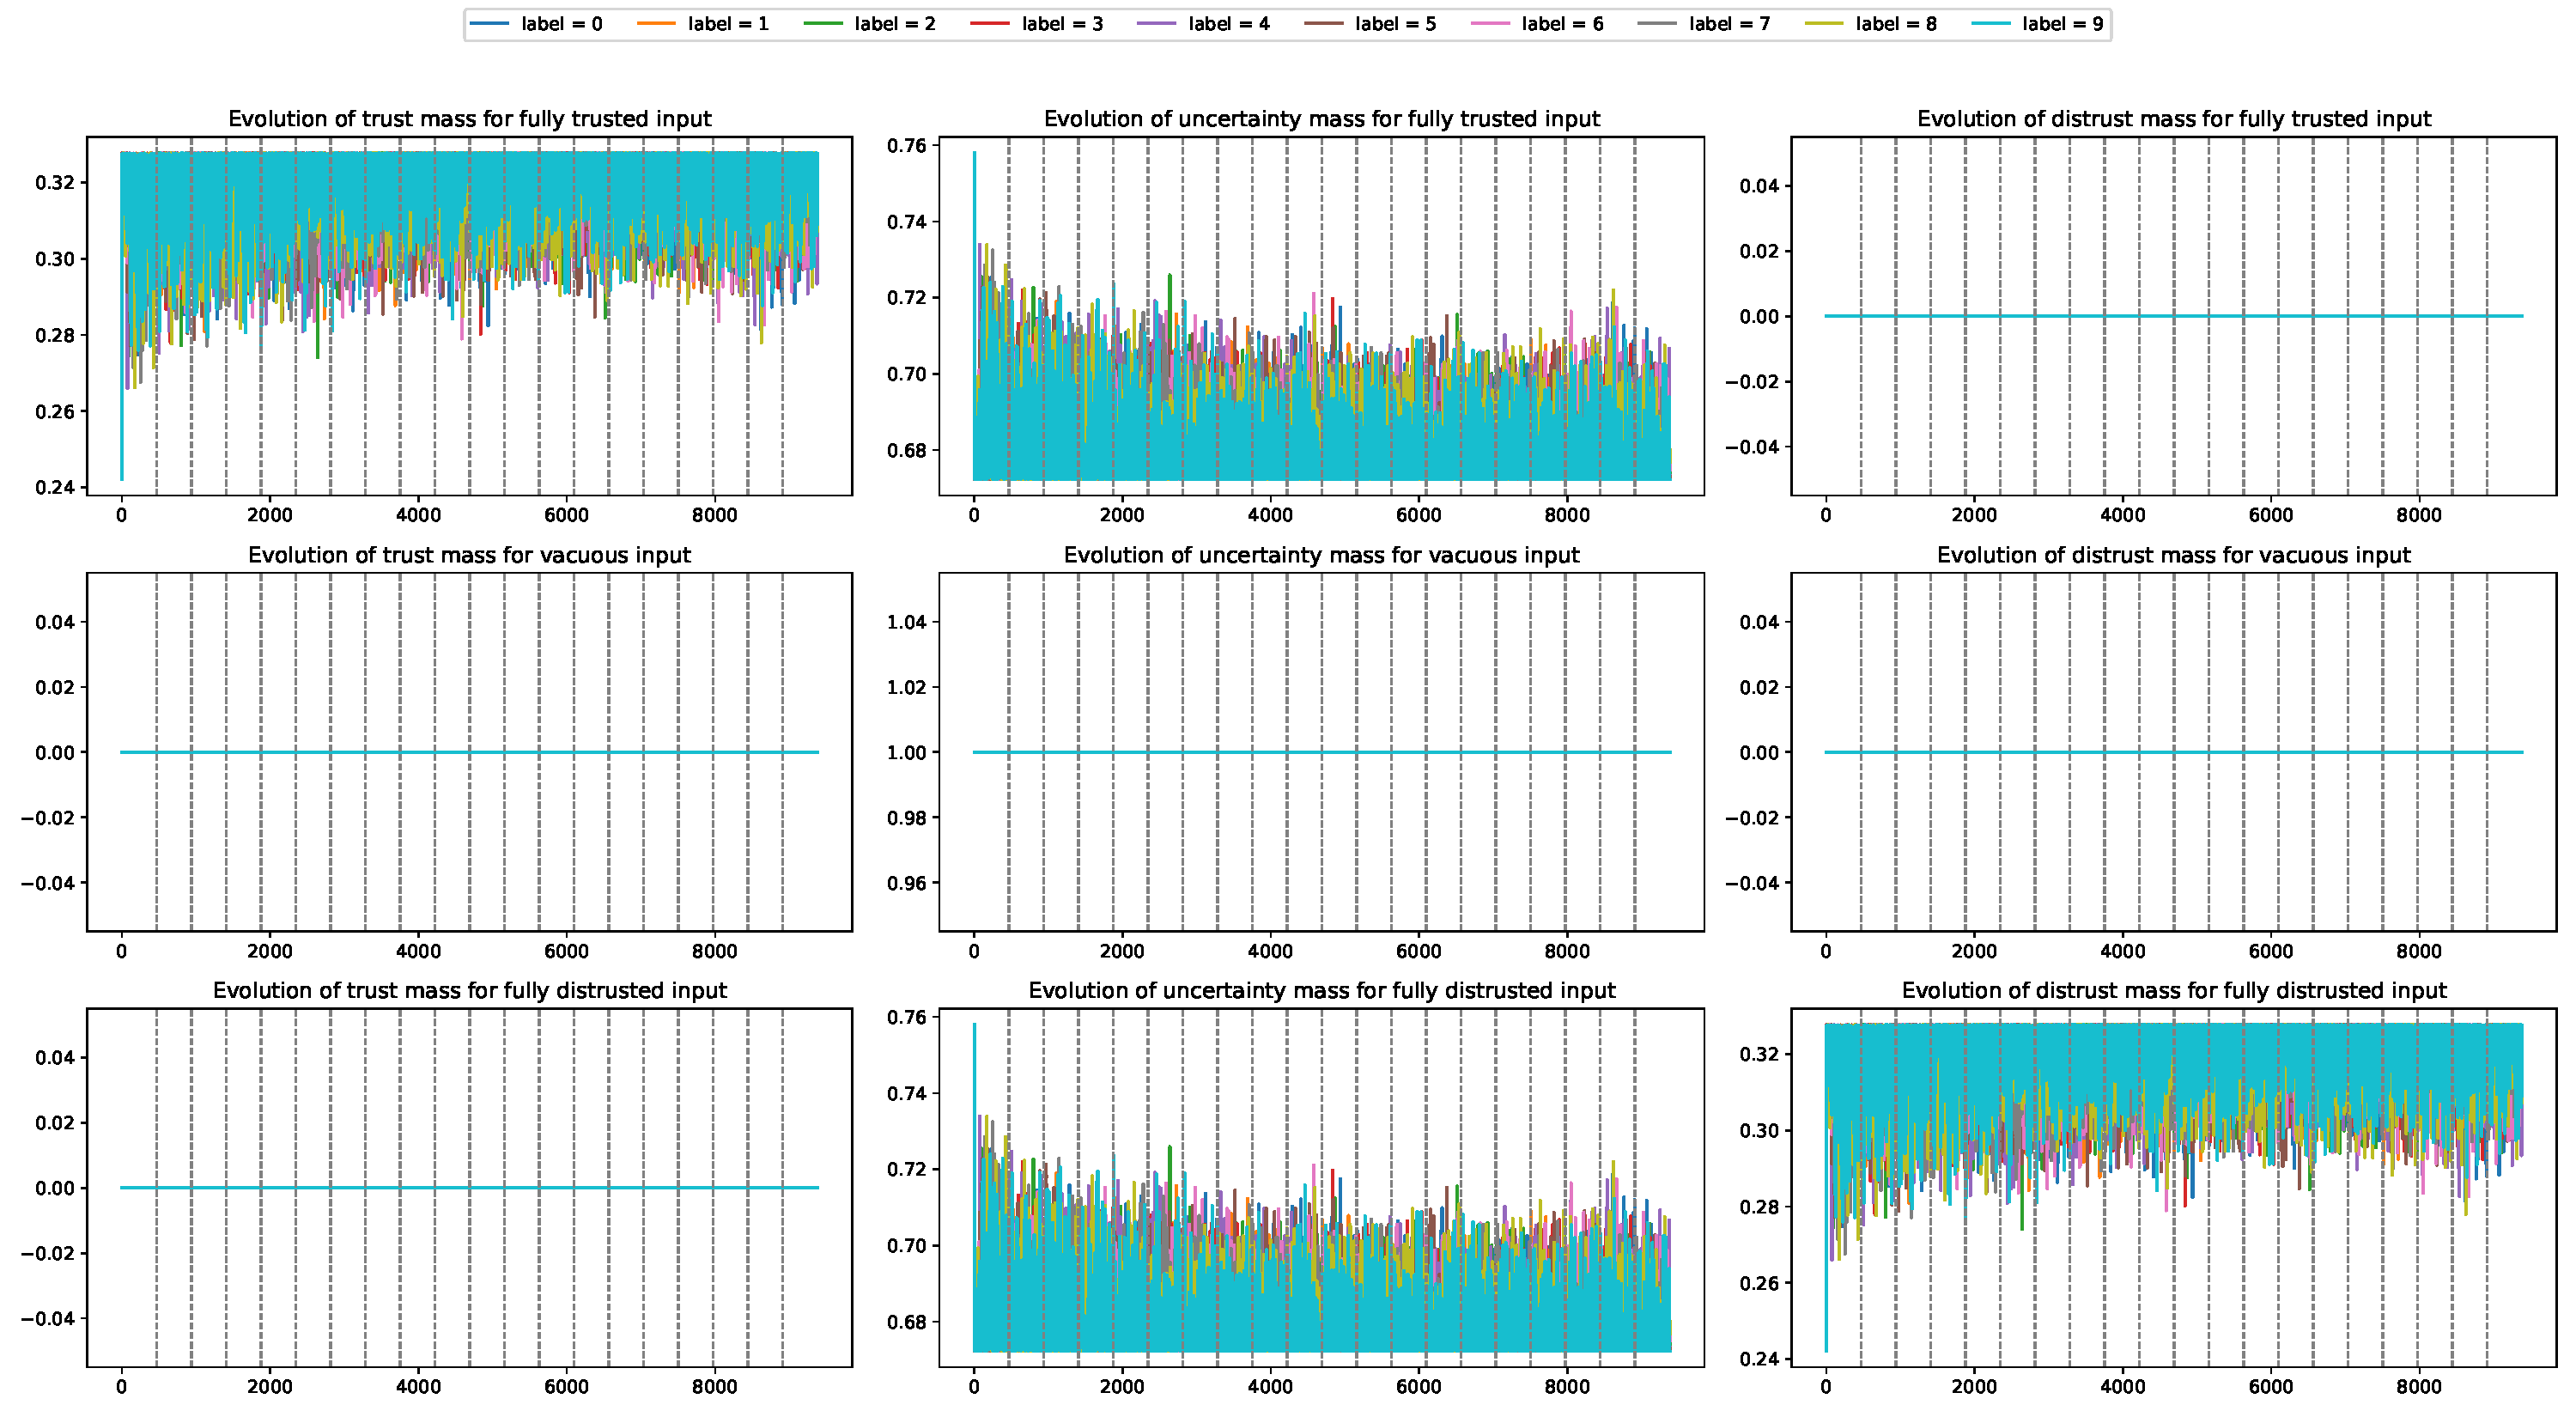
\includegraphics[width=\textwidth]{plots_v2/MNIST/architecture/plot_ptas-32-v-v.pdf}
  \caption{32 Hidden neurons}
\end{figure}
\begin{figure}[H]
  \centering
  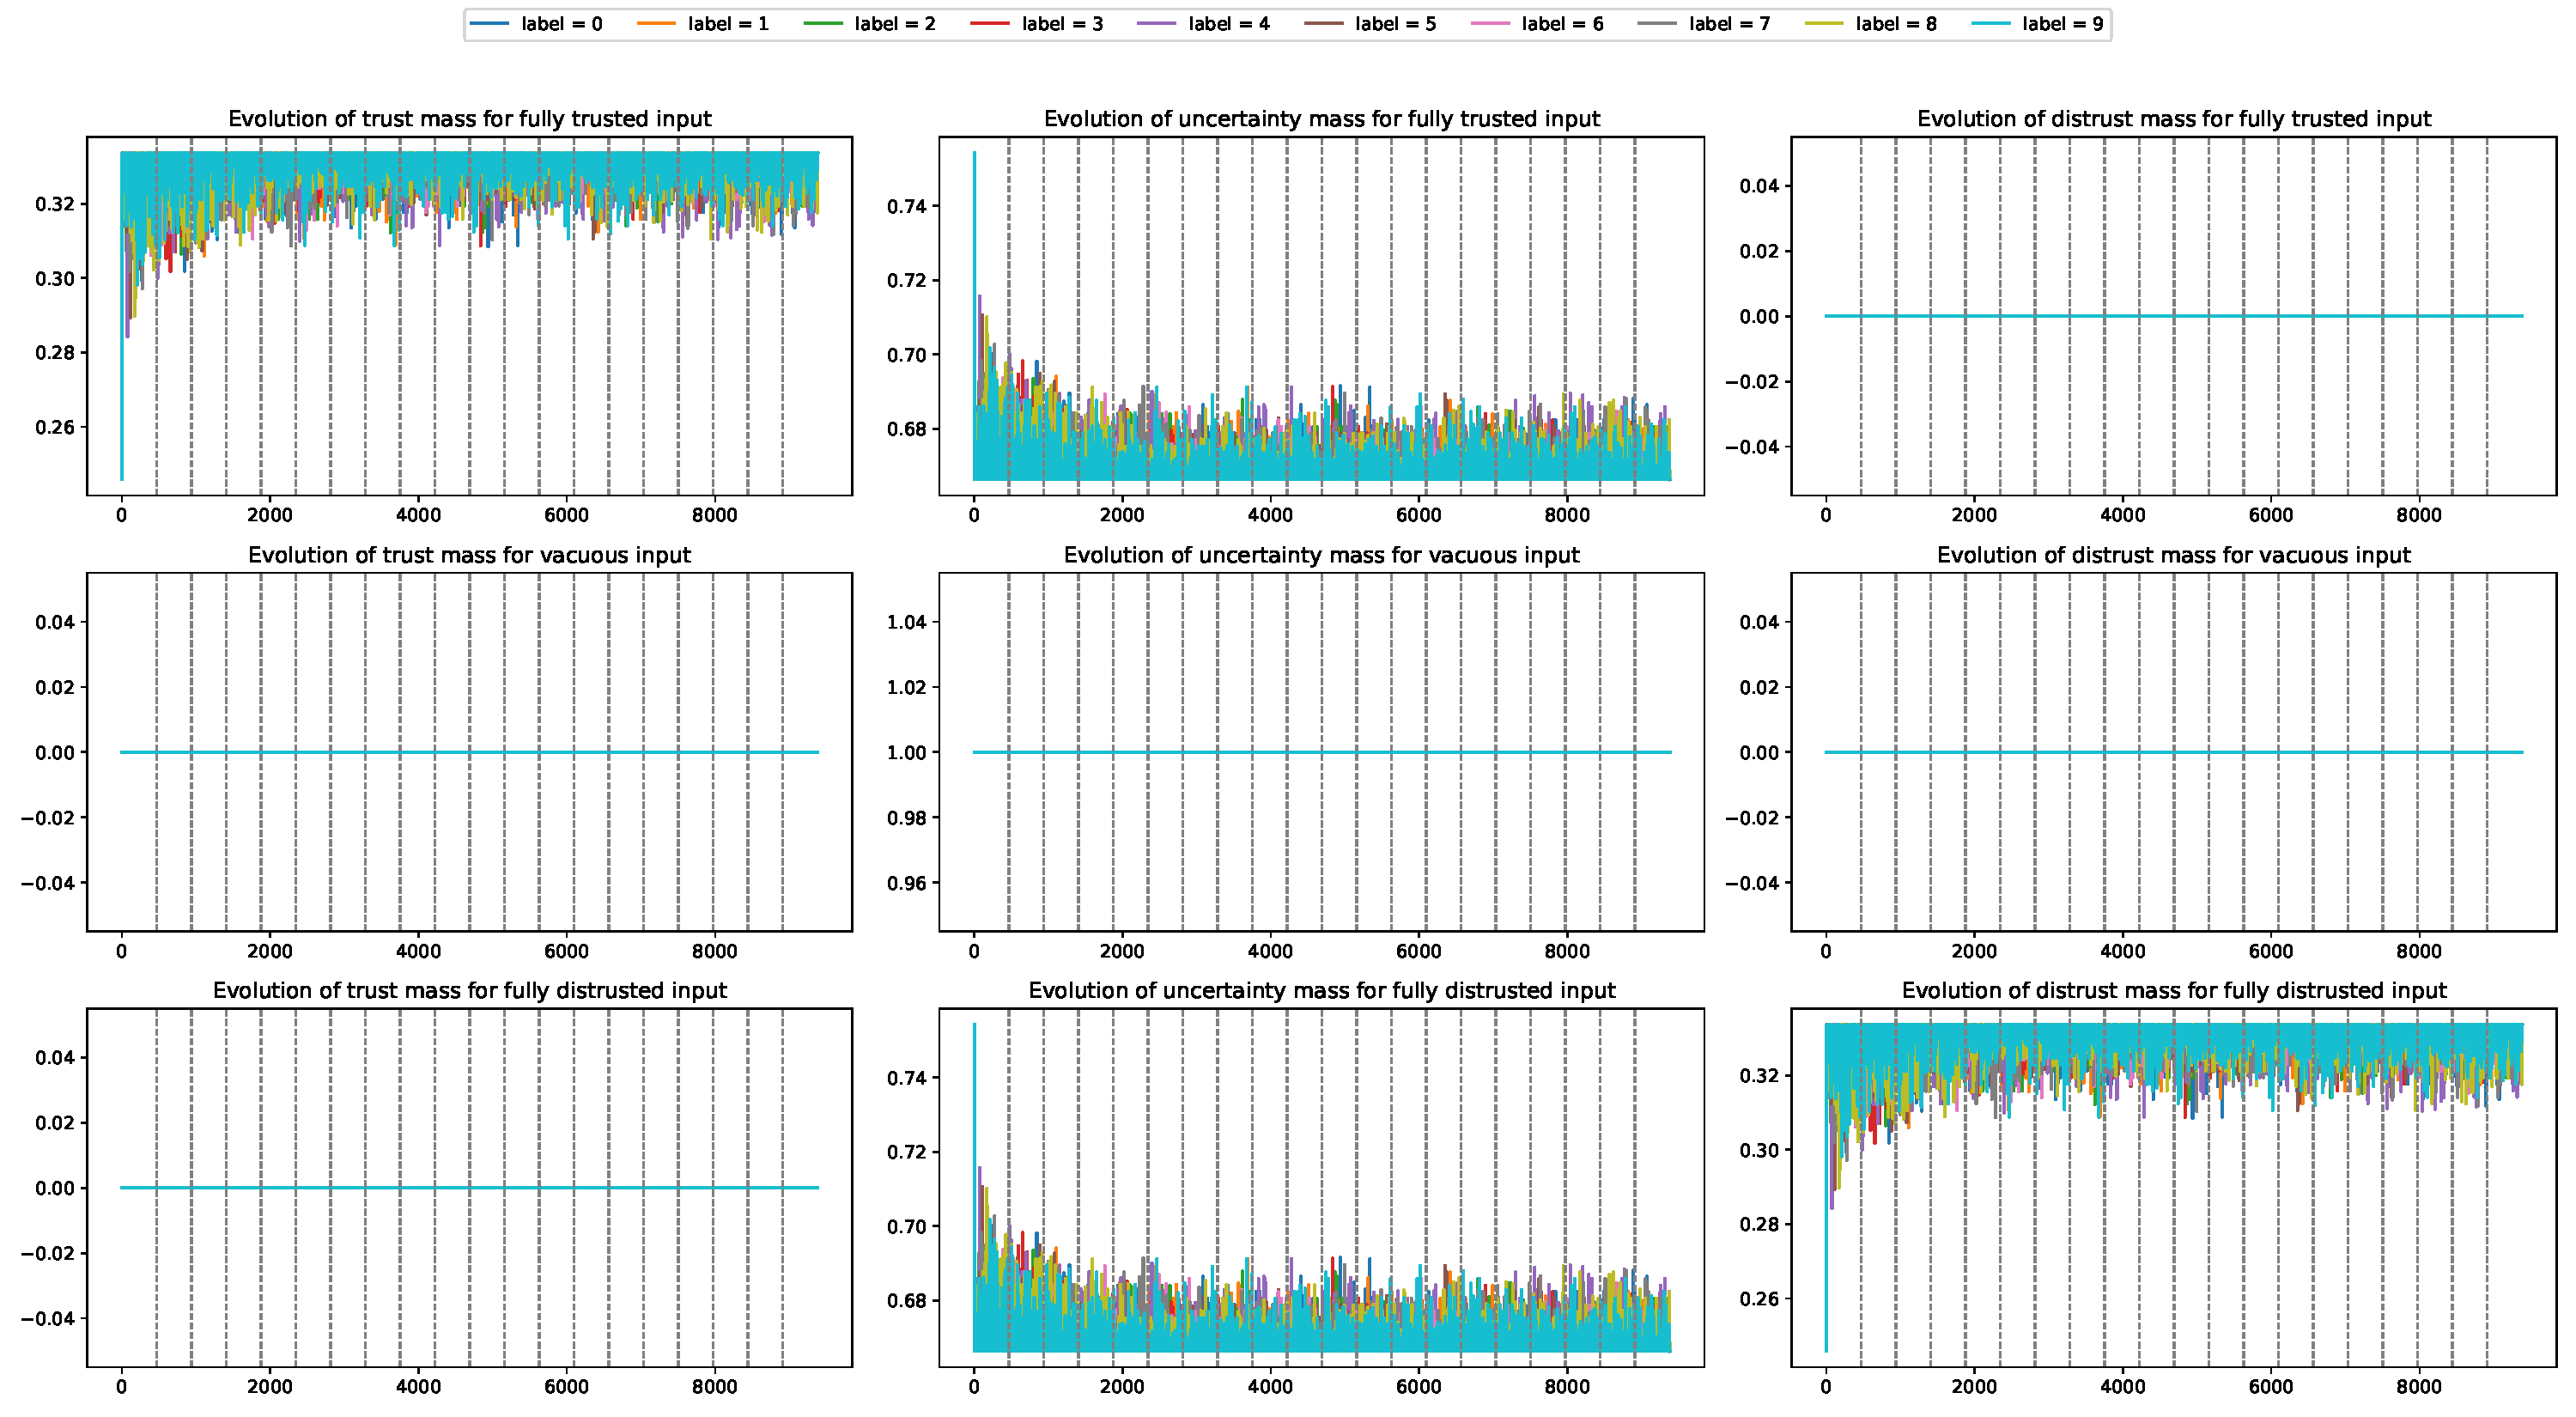
\includegraphics[width=\textwidth]{plots_v2/MNIST/architecture/plot_ptas-64-v-v.pdf}
  \caption{64 Hidden neurons}
\end{figure}
\begin{figure}[H]
  \centering
  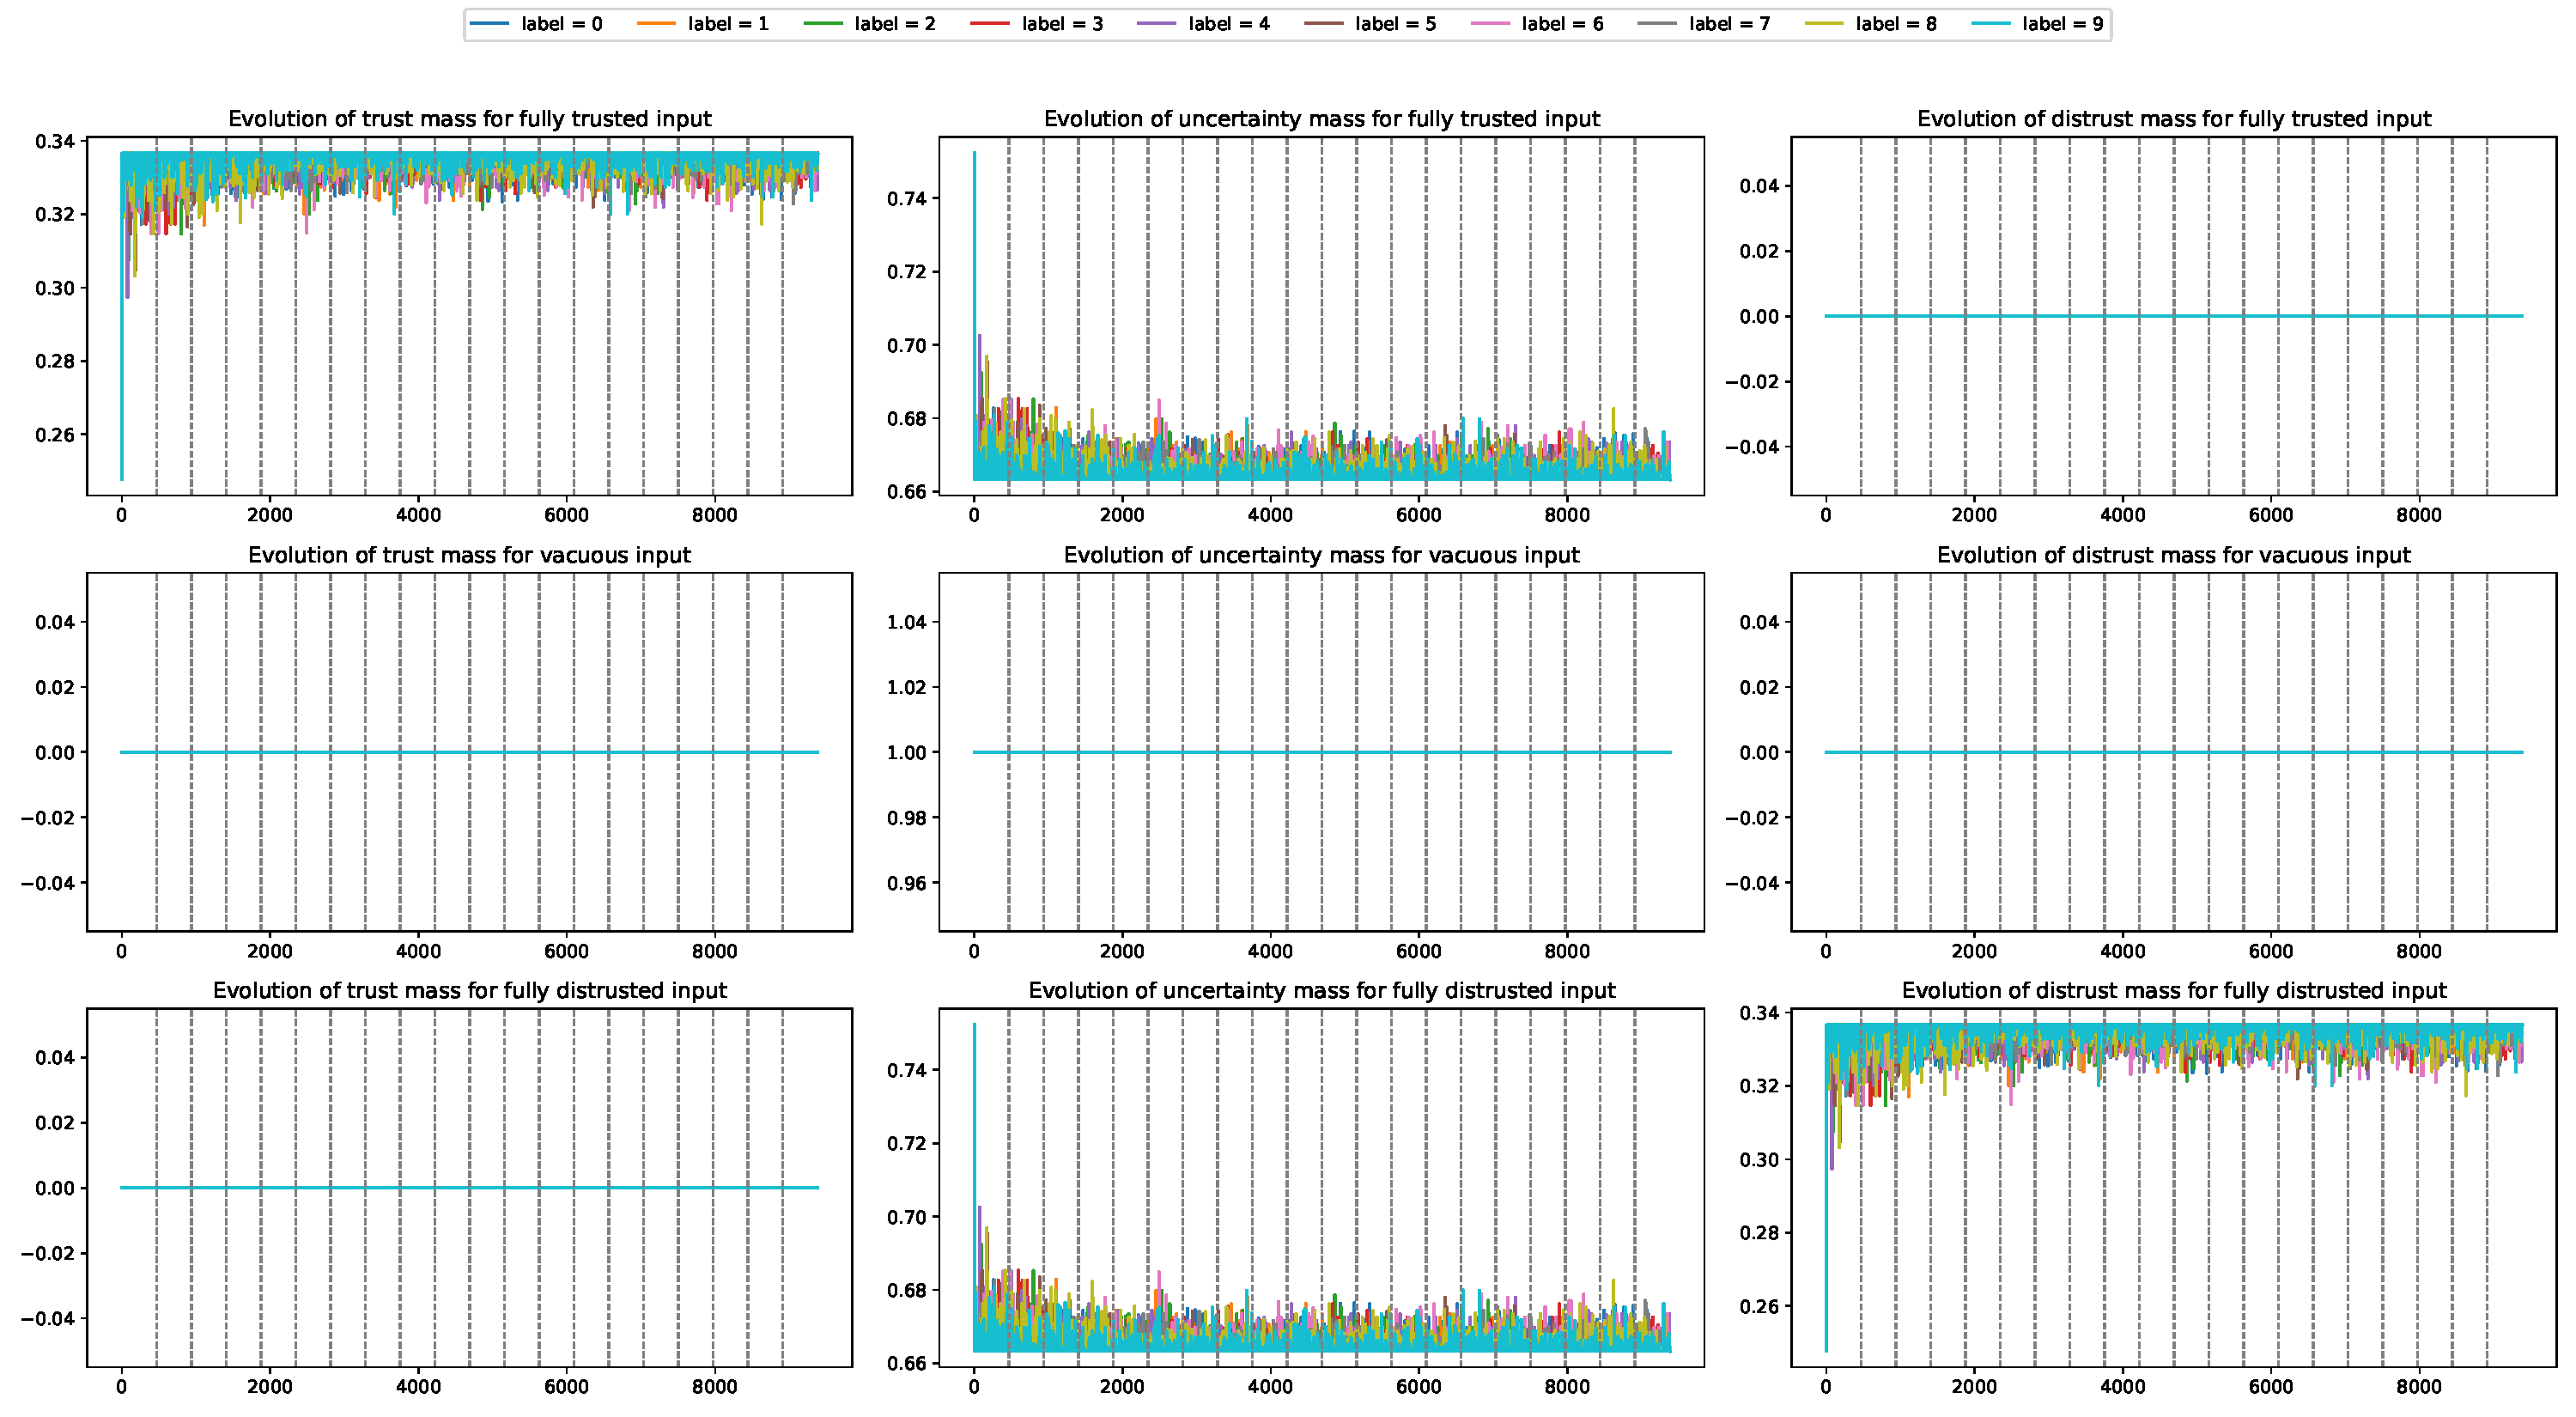
\includegraphics[width=\textwidth]{plots_v2/MNIST/architecture/plot_ptas-128-v-v.pdf}
  \caption{128 Hidden neurons}
\end{figure}
\begin{figure}[H]
  \centering
  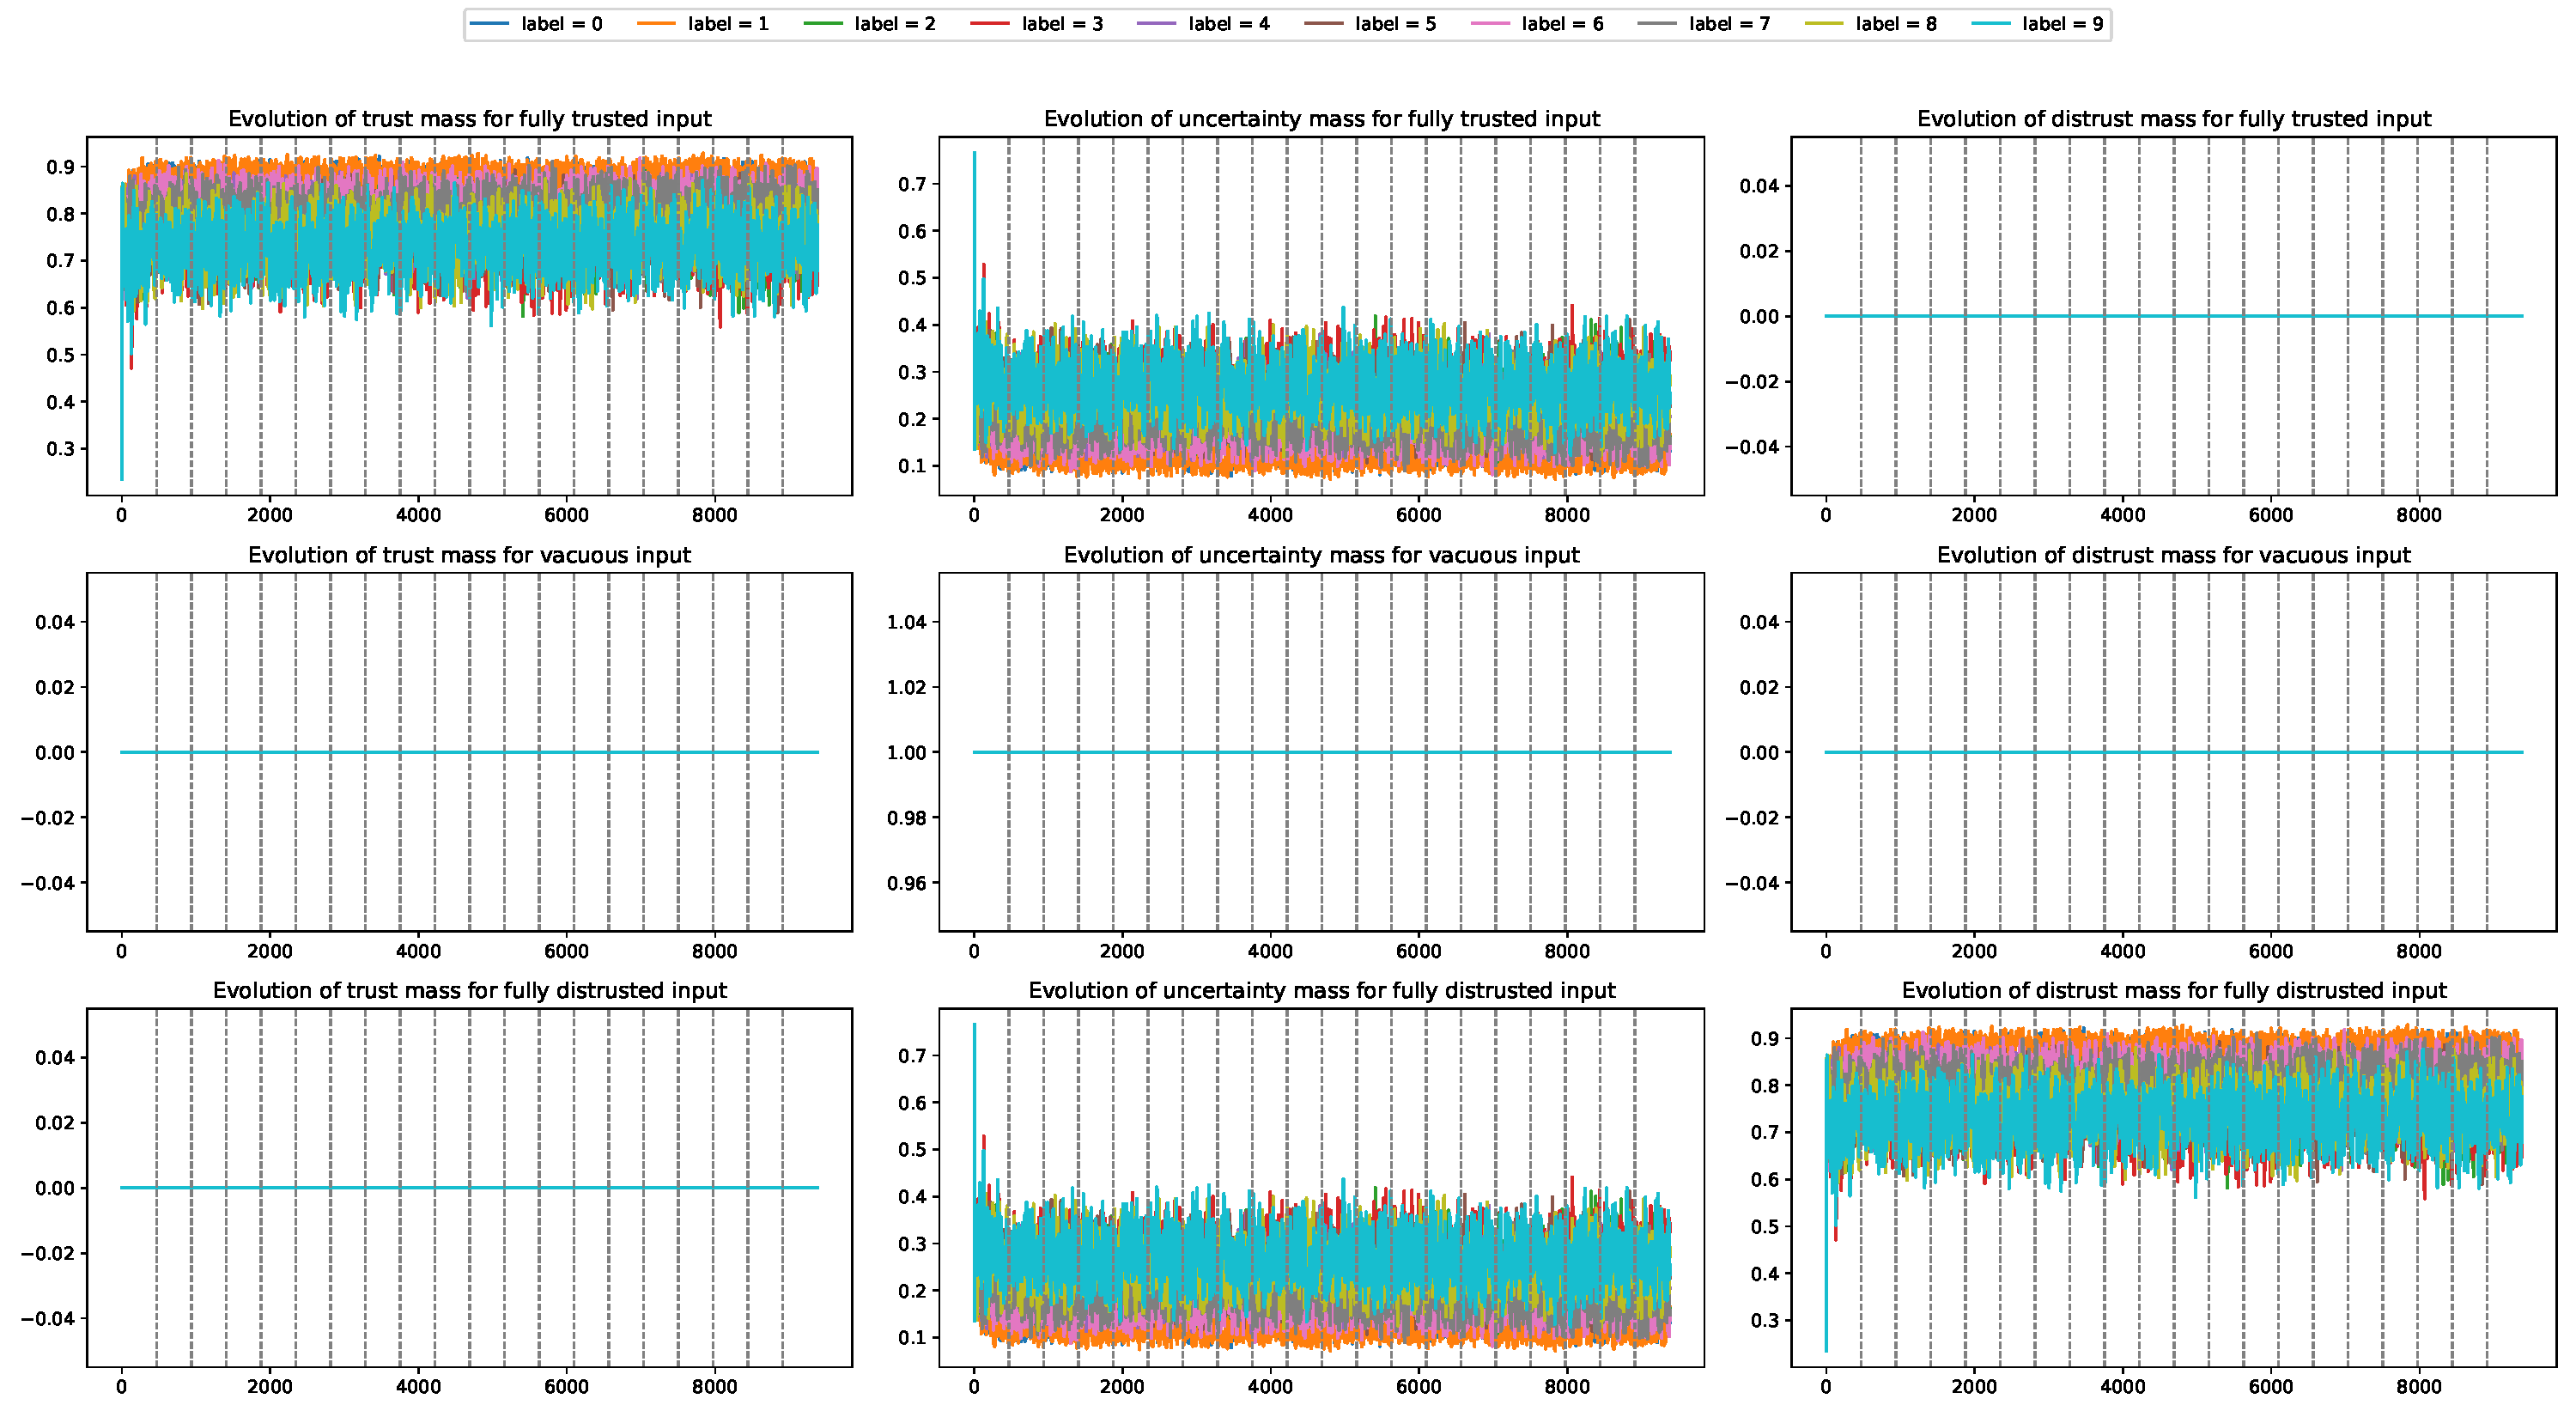
\includegraphics[width=\textwidth]{plots_v2/MNIST/architecture/plot_ptas-16-t-t.pdf}
  \caption{16 Hidden neurons with Fully Trusted Assessment}
\end{figure}

\subsection{MNIST poisoned 128 hidden neurons (\cref{exp:3})}\label{sec:resmnistpois}
\begin{figure}[H]
  \centering
  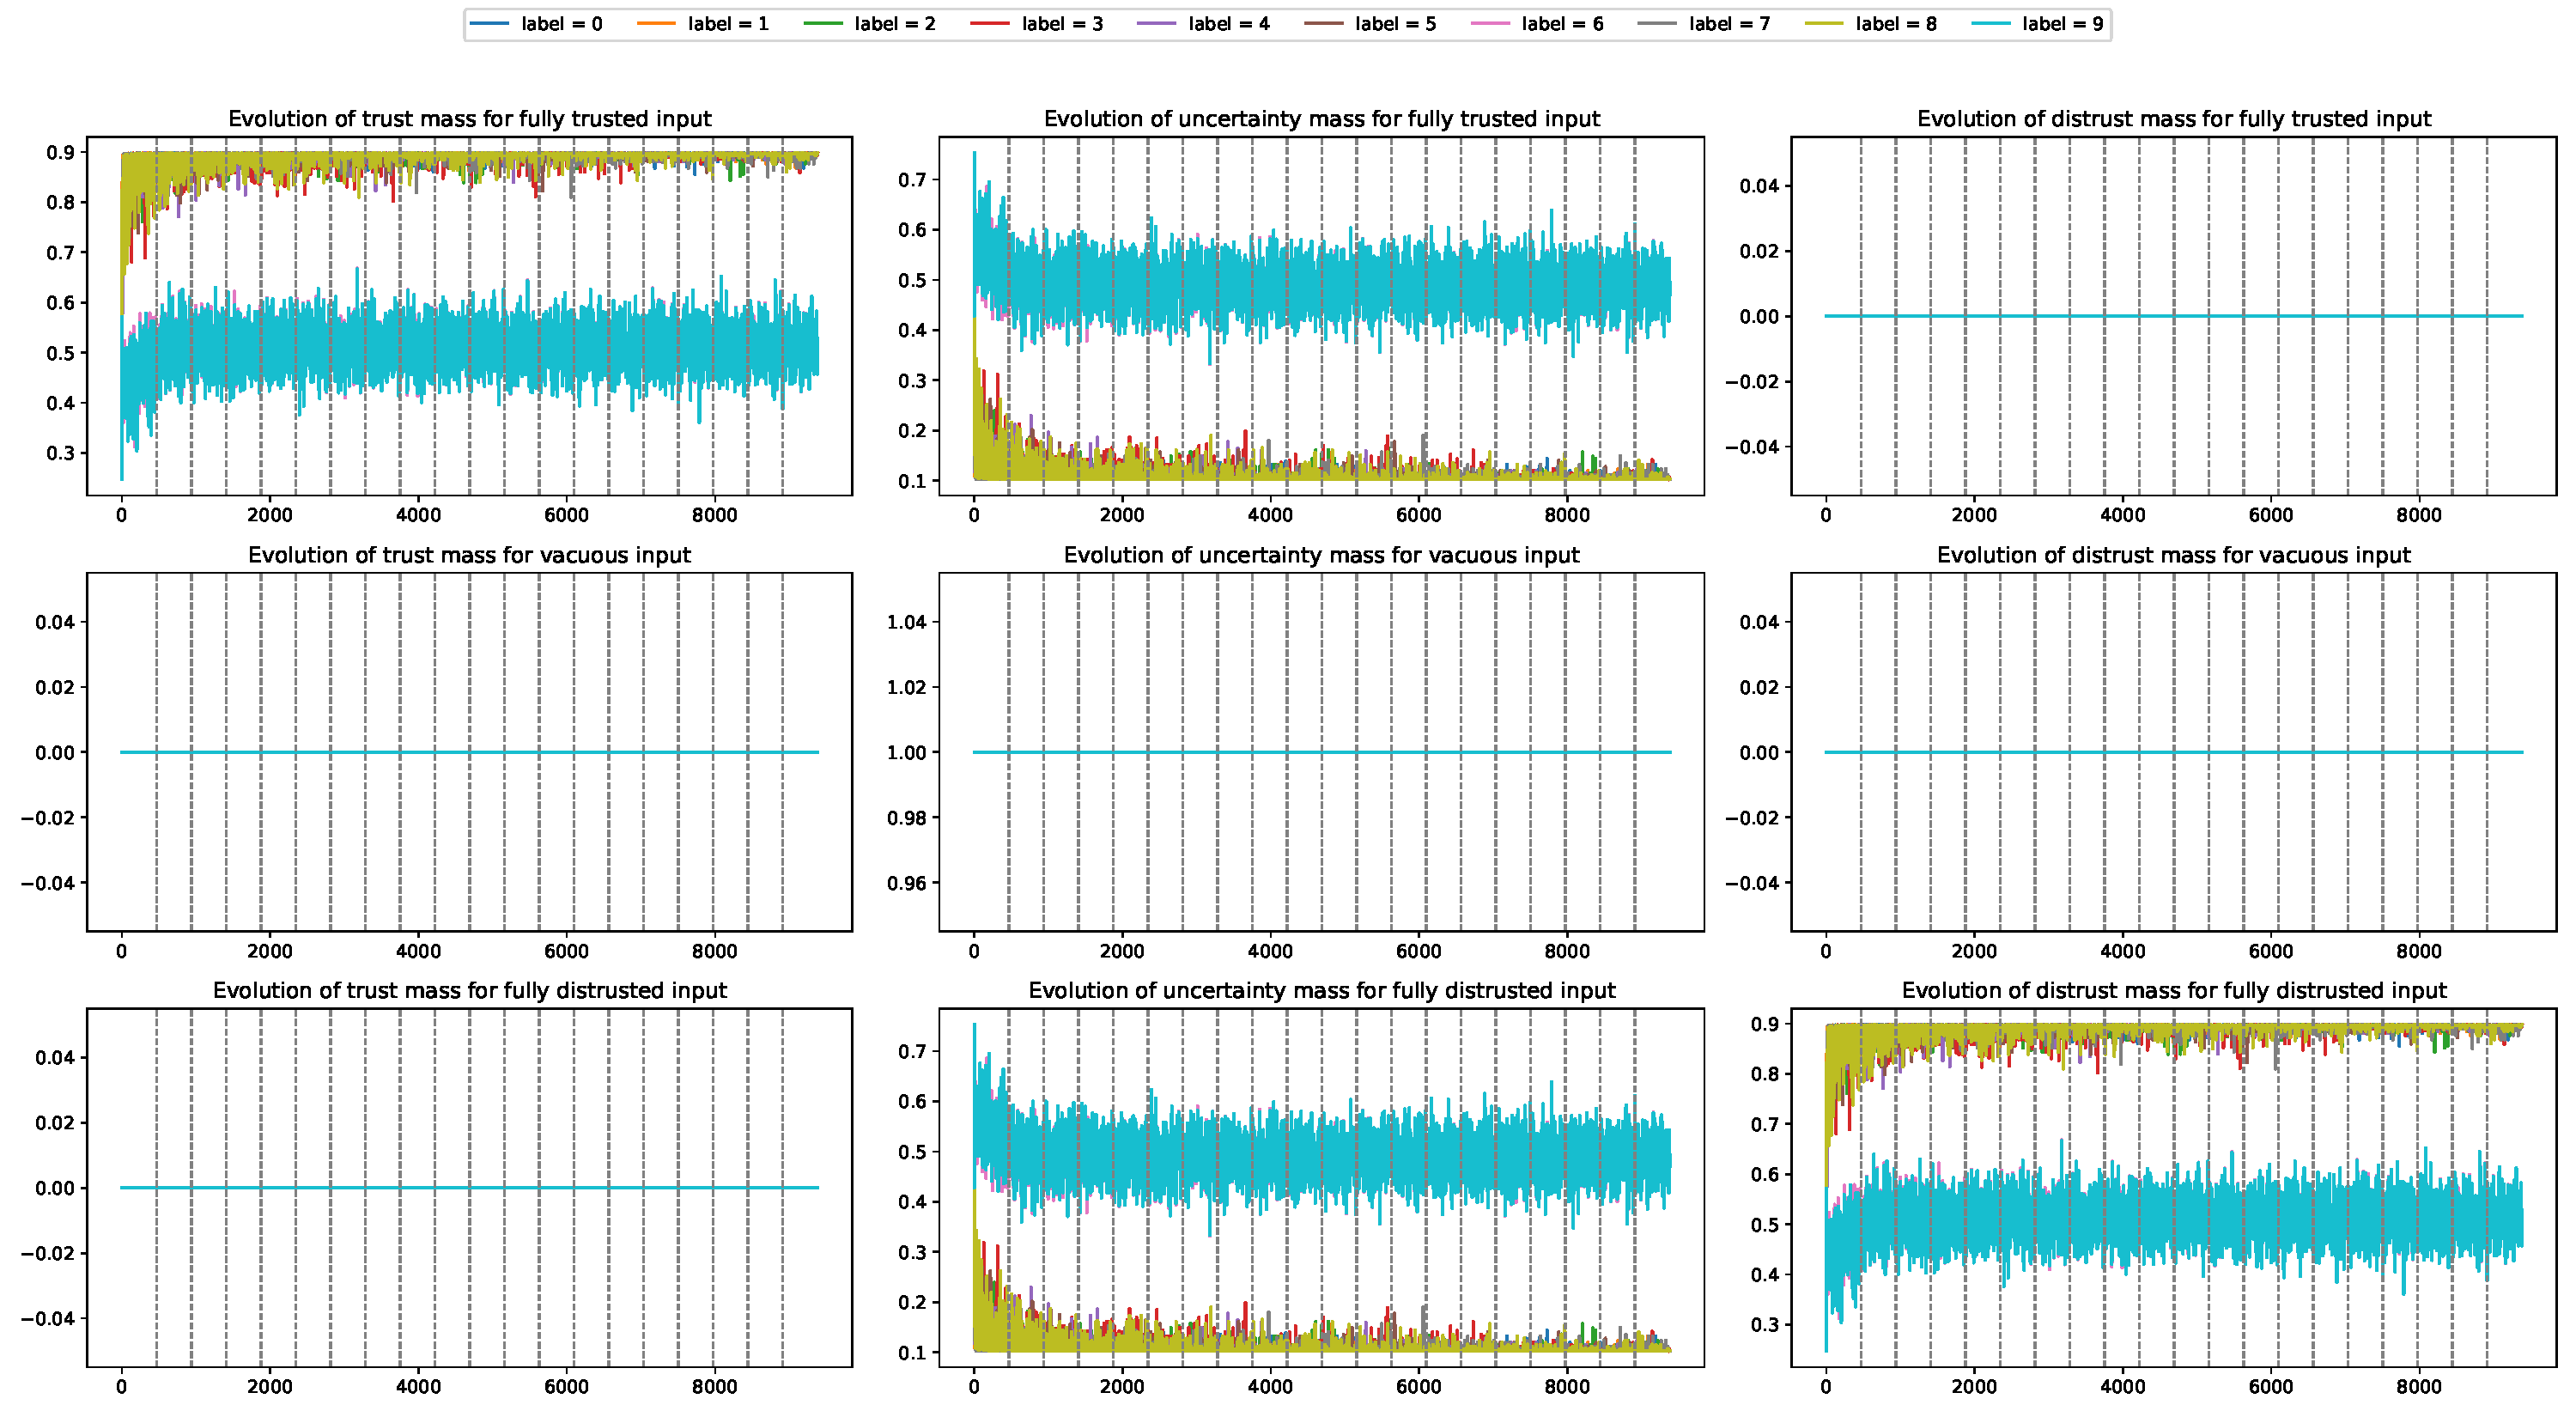
\includegraphics[width=\textwidth]{plots_v2/MNIST/poisoned/plot_ptas-128-t-t-ps1.pdf}
  \caption{1 pixel}
\end{figure}
\begin{figure}[H]
  \centering
  \includegraphics[width=\textwidth]{plots_v2/MNIST/poisoned/plot_ptas-128-t-t-ps4.pdf}
  \caption{4×4 pixels}
\end{figure}
\begin{figure}[H]
  \centering
  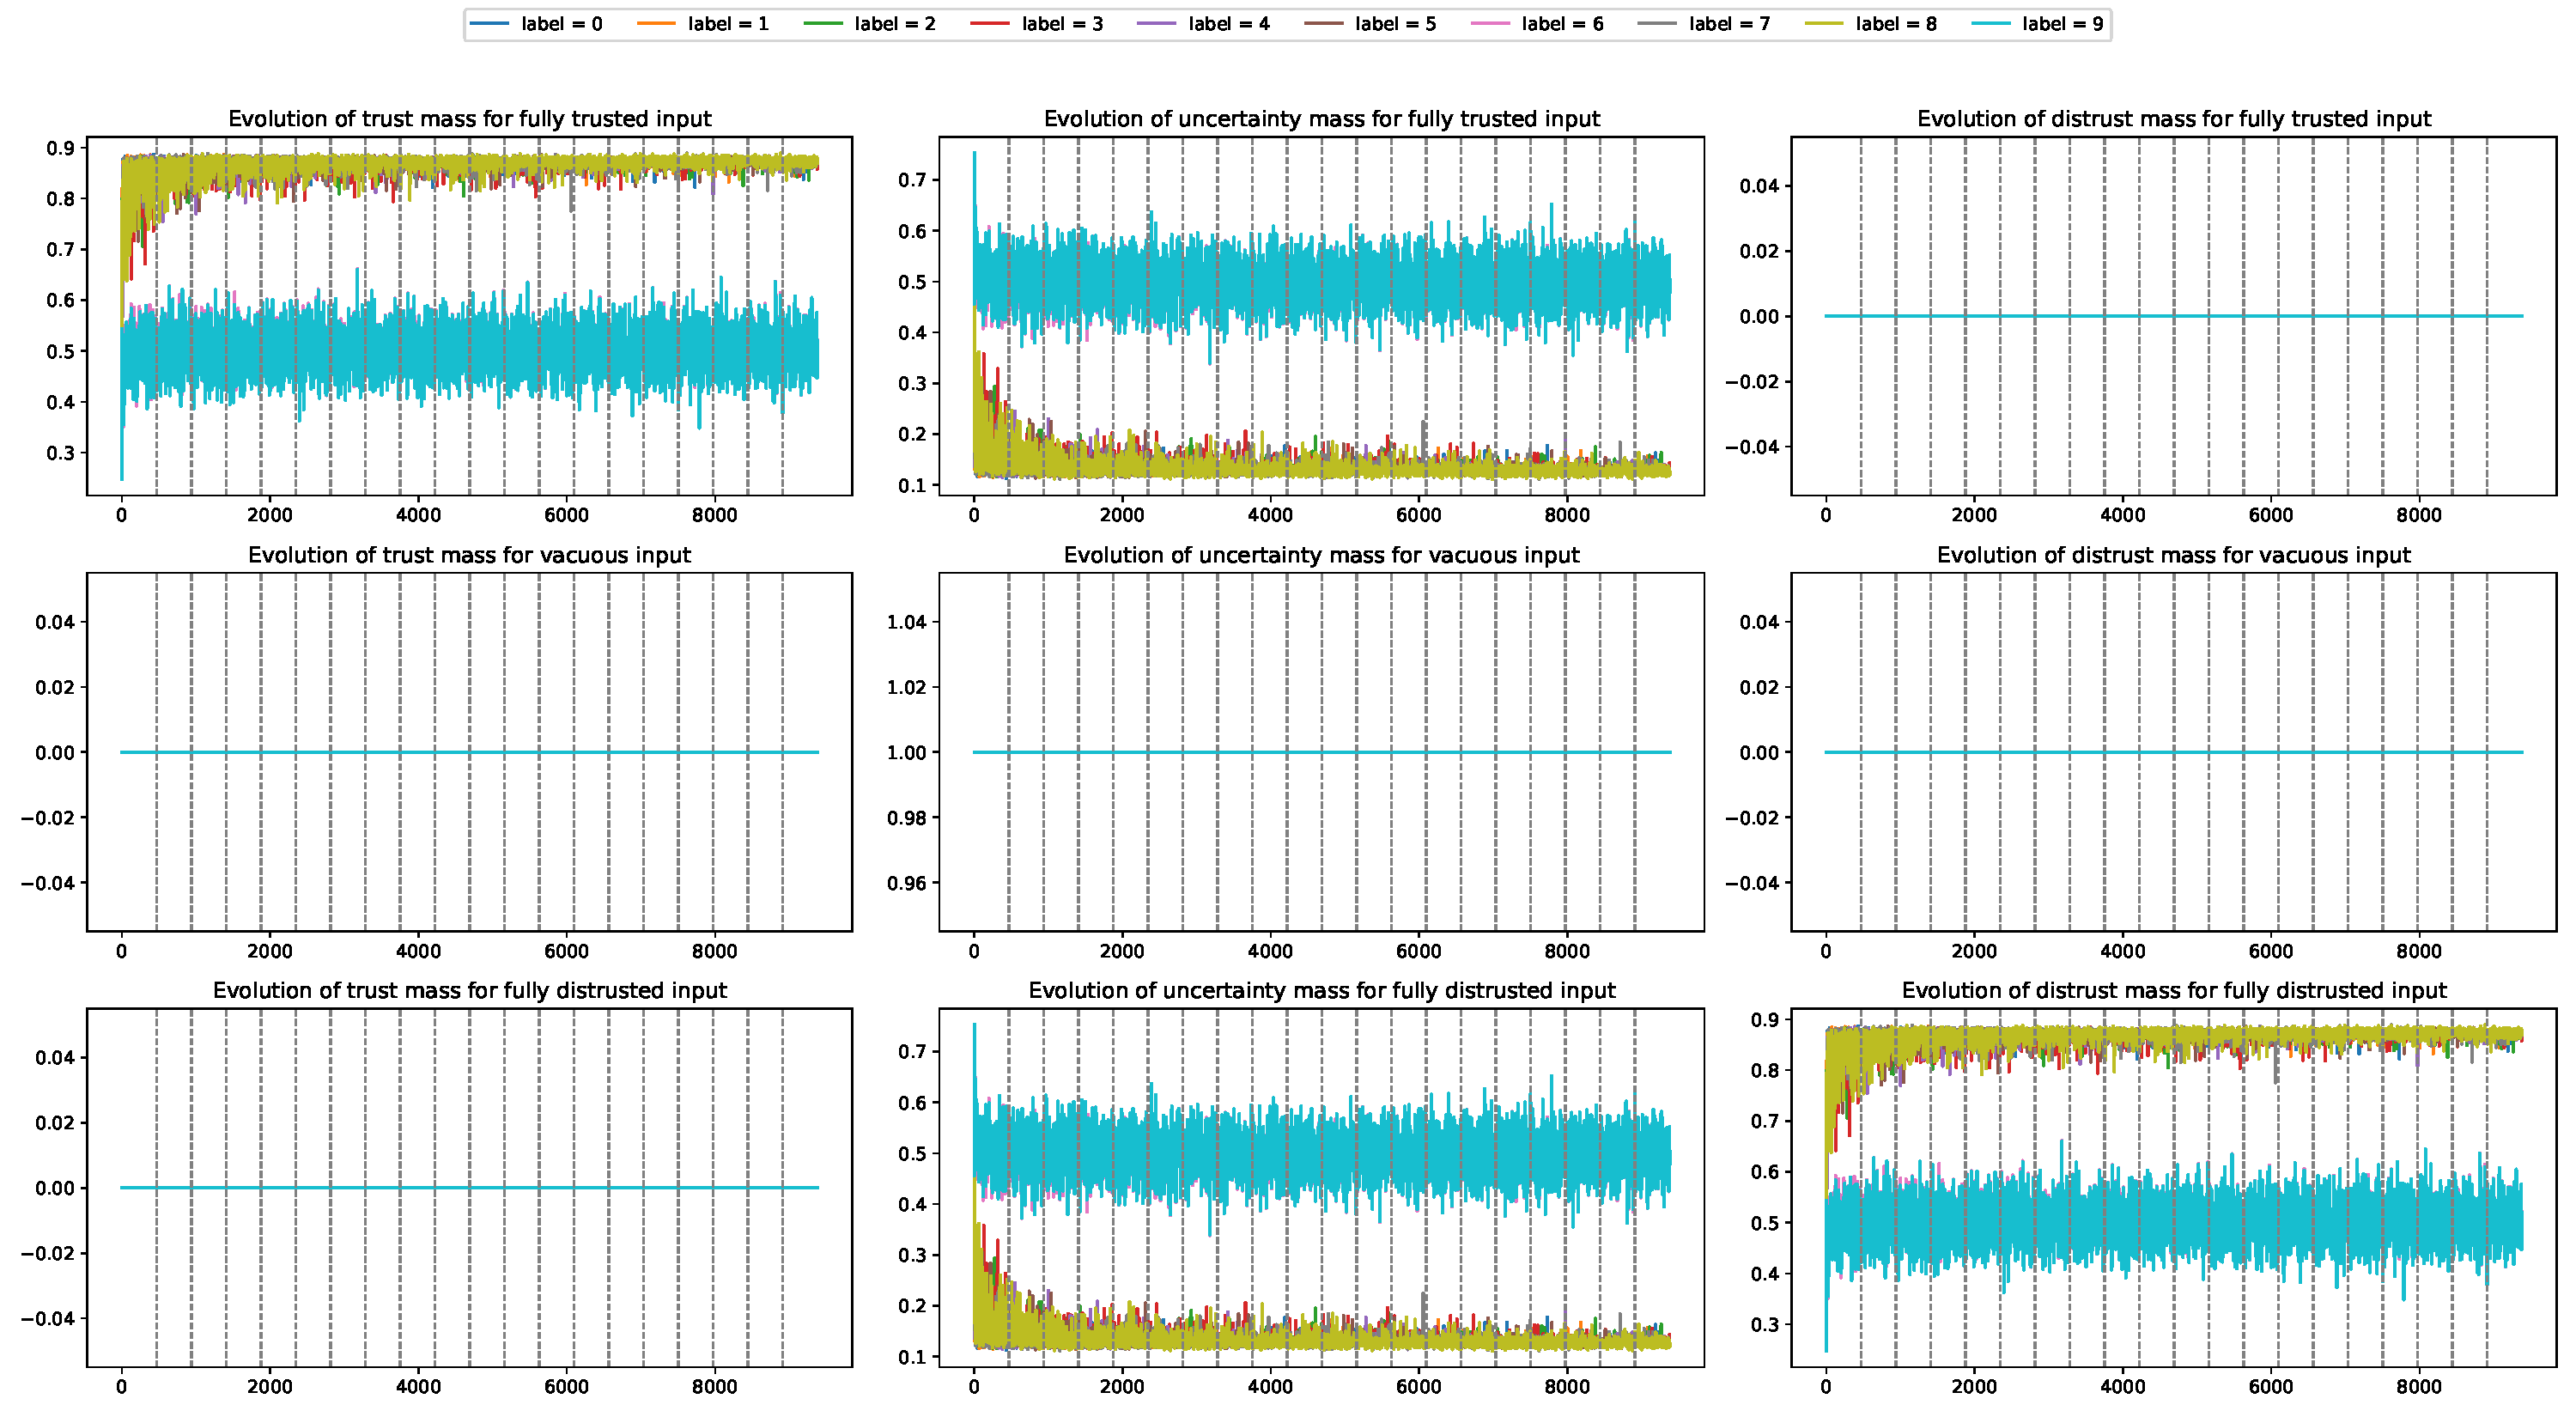
\includegraphics[width=\textwidth]{plots_v2/MNIST/poisoned/plot_ptas-128-t-t-ps10.pdf}
  \caption{10×10 pixels}
\end{figure}
\begin{figure}[H]
  \centering
  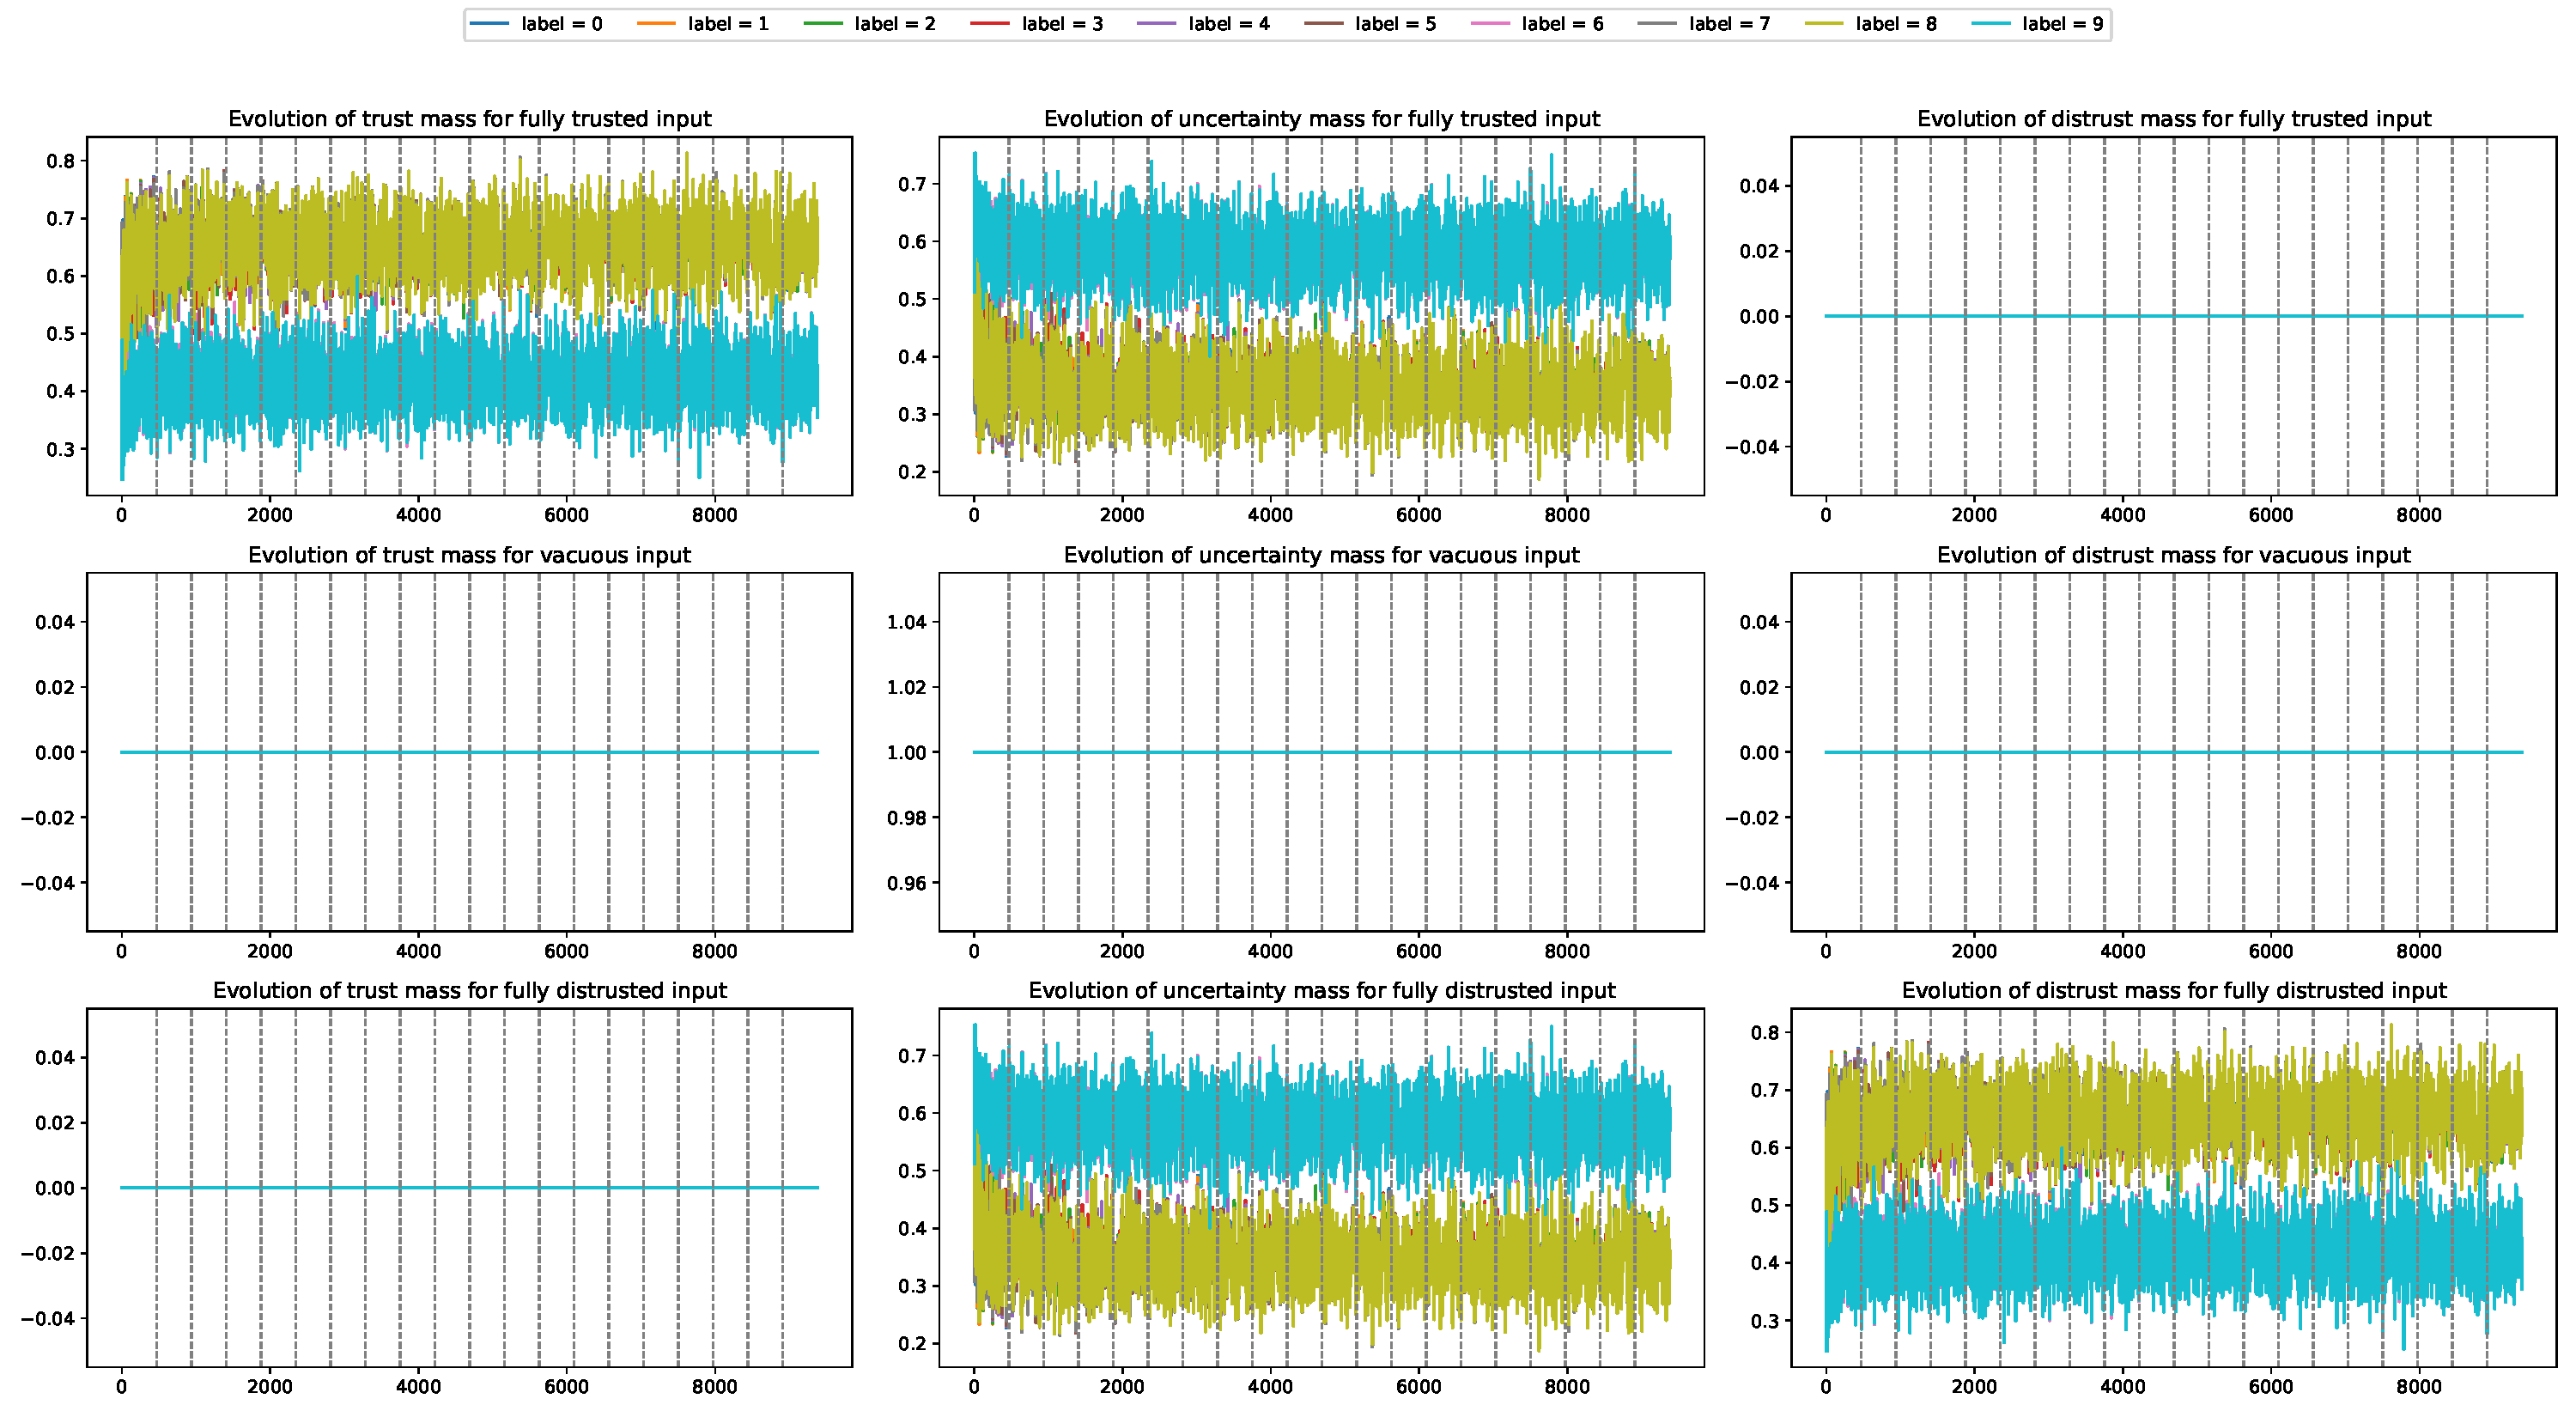
\includegraphics[width=\textwidth]{plots_v2/MNIST/poisoned/plot_ptas-128-t-t-ps27.pdf}
  \caption{27×27 pixels}
\end{figure}
\subsection{Plots for the Comparative Trust Evaluation (\cref{exp:4})}\label{sec:resexp4}
\begin{figure}[H]
  \centering
  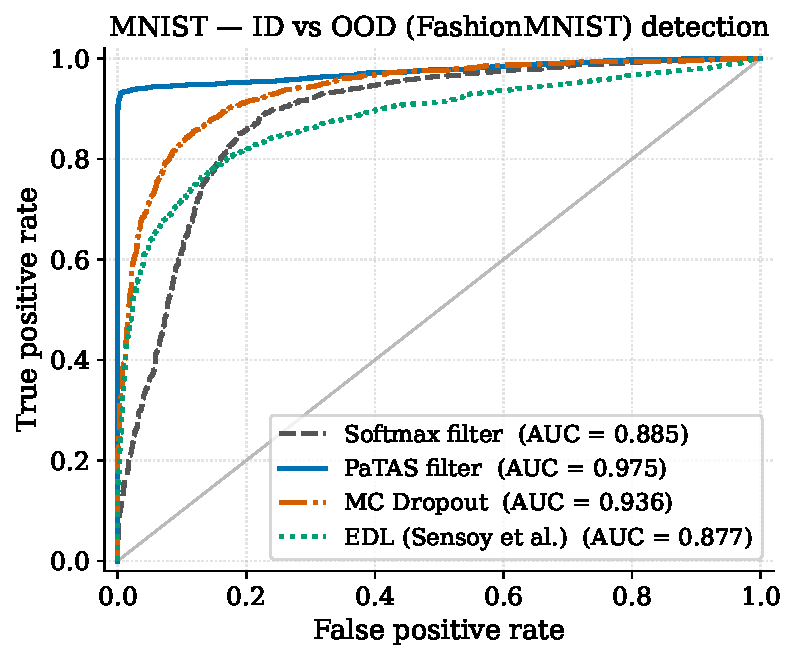
\includegraphics[width=0.62\textwidth]{plots_v2/exp4/roc_ood_mnist.pdf}
  \caption{Out-of-distribution detection ROC (MNIST in-distribution vs.\ Fashion-MNIST OOD): each method's own score as the discriminator. Curves and legend AUC values are from a single representative evaluation seed; \cref{tab:comparative} reports mean $\pm$ std over three seeds.}
\end{figure}
\begin{figure}[H]
  \centering
  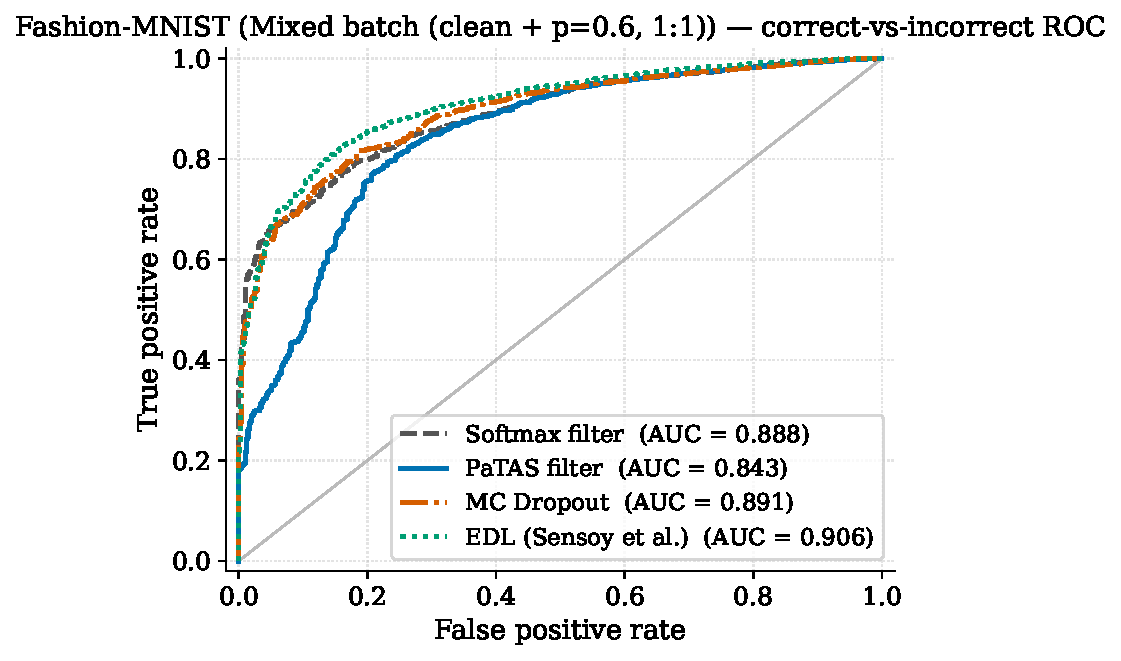
\includegraphics[width=0.62\textwidth]{plots_v2/exp4/roc_mixed_fashion.pdf}
  \caption{Correct-vs-incorrect ROC on the Fashion-MNIST mixed batch (clean + corrupted inputs pooled 1:1), single representative evaluation seed.}
\end{figure}
\begin{figure}[H]
  \centering
  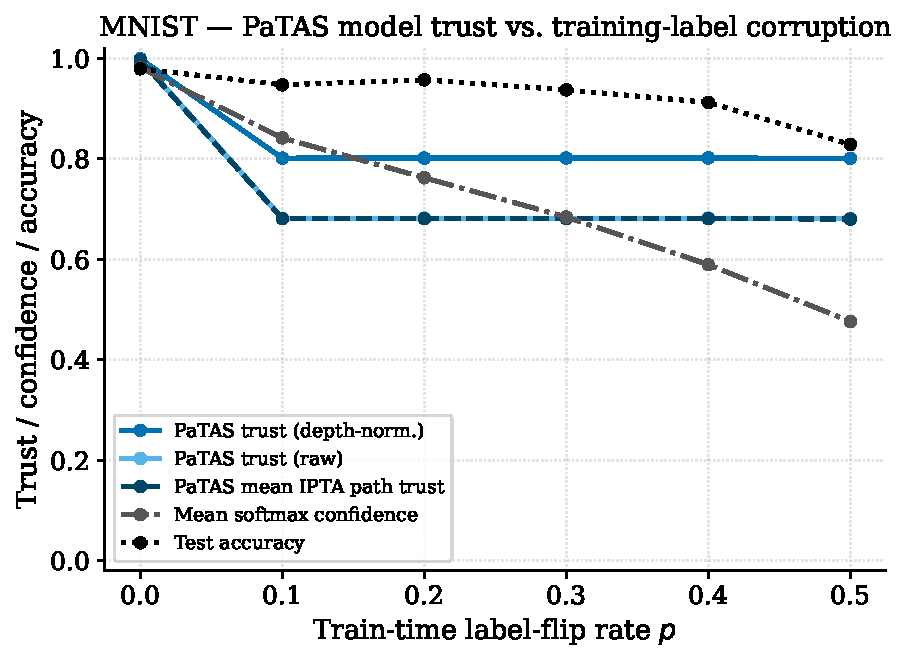
\includegraphics[width=0.62\textwidth]{plots_v2/exp4/model_trust_vs_labelnoise.pdf}
  \caption{Training-quality audit (\cref{tab:audit}): PaTAS model-side trust, mean softmax confidence, and test accuracy as functions of the train-time label-flip rate $p$. The depth-normalized curve rescales the committed mass $b+d$ of the aggregated opinion to $(b+d)^{1/L}$, with $L$ the number of trust-propagation layers, making trust comparable across network depths. Trust drops as a tripwire at any non-zero rate without using test data; confidence tracks severity but requires a clean labelled test set.}
\end{figure}

\subsection{Example for random dataset trust assessment}\label{sec:resrand}

\begin{figure}[H]
\centering
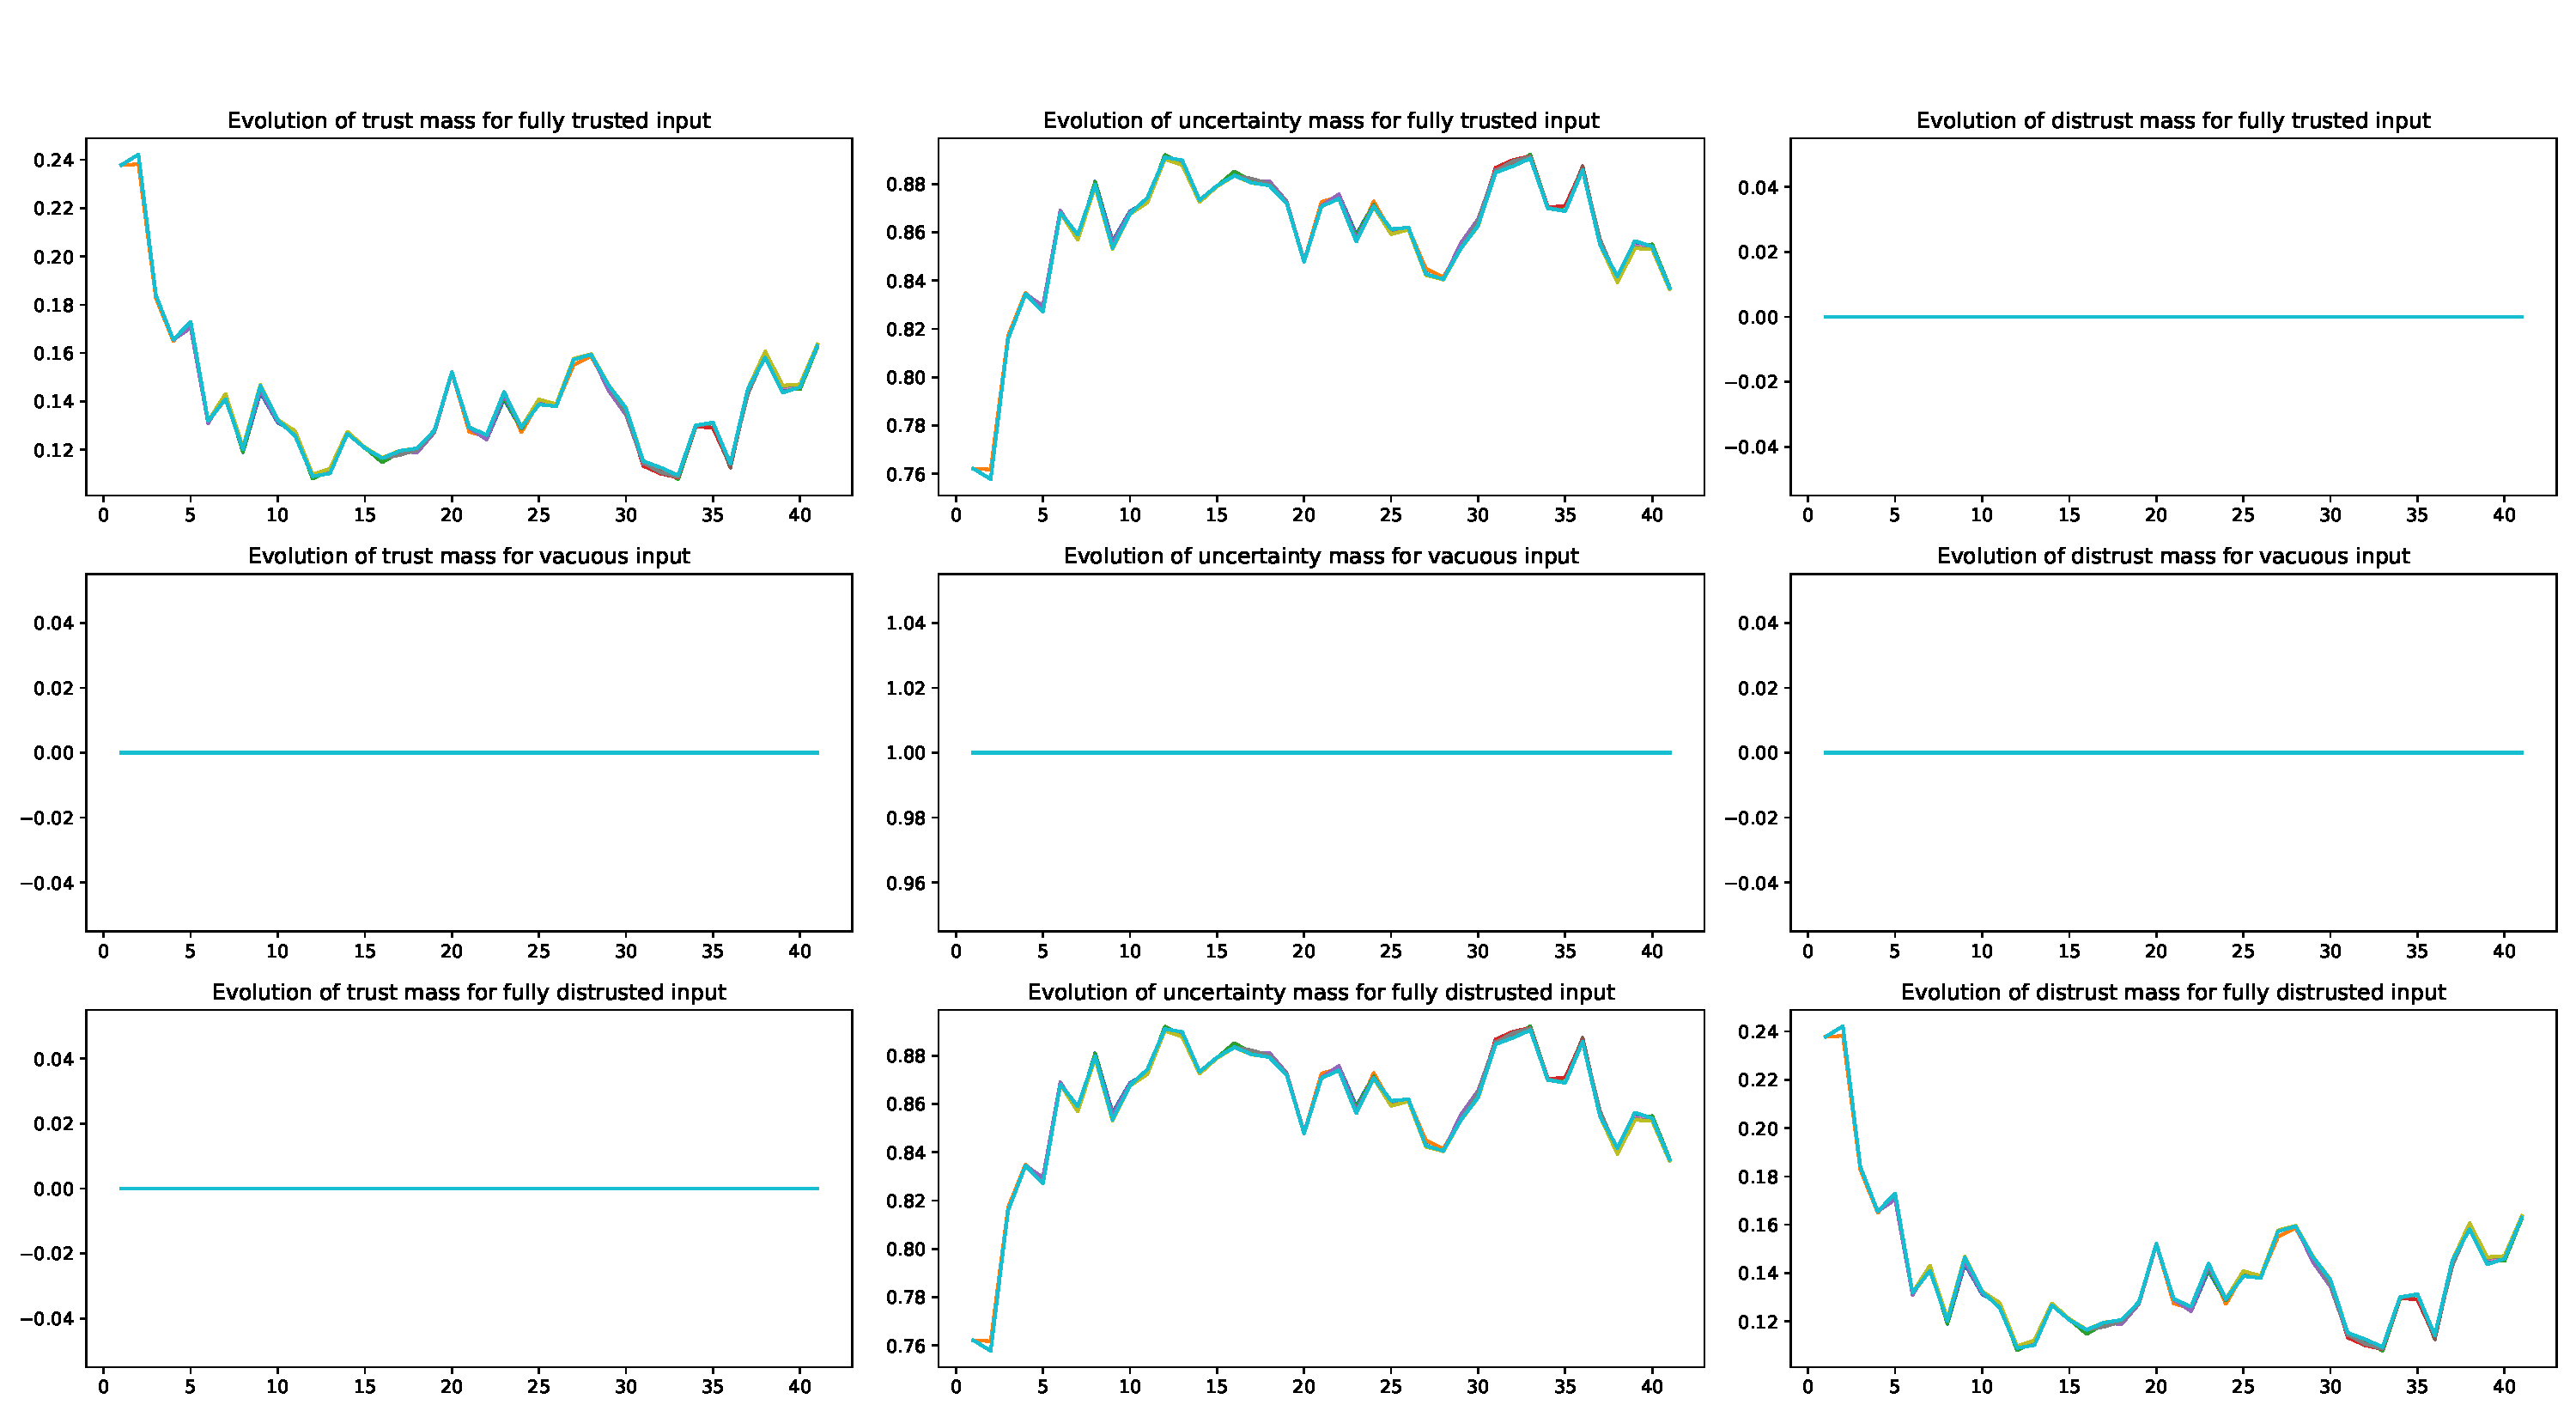
\includegraphics[width=\textwidth]{plots_v2/randomMNIST/all.pdf}
\caption{MNIST randomized trust}
\label{fig:mnistrand}
\end{figure}



% \subsection{Plots for Cancer Model with \(\epsilon = 0.01\) (\cref{exp:1})}\label{sec:rescancer0.01}
\begin{figure}[H]
  \includegraphics[width=\textwidth]{plots_v2/Cancer/eps=0.01/plot_ptas-d-d.pdf}
  \caption{Features distrusted and labels distrusted}
\end{figure}
\begin{figure}[H]
  \includegraphics[width=\textwidth]{plots_v2/Cancer/eps=0.01/plot_ptas-d-v.pdf}
  \caption{Features distrusted and labels vacuous}
\end{figure}
\begin{figure}[H]
  \includegraphics[width=\textwidth]{plots_v2/Cancer/eps=0.01/plot_ptas-d-t.pdf}
  \caption{Features distrusted and labels trusted}
\end{figure}
\begin{figure}[H]
  \includegraphics[width=\textwidth]{plots_v2/Cancer/eps=0.01/plot_ptas-v-d.pdf}
  \caption{Features vacuous and labels distrusted}
\end{figure}
\begin{figure}[H]
  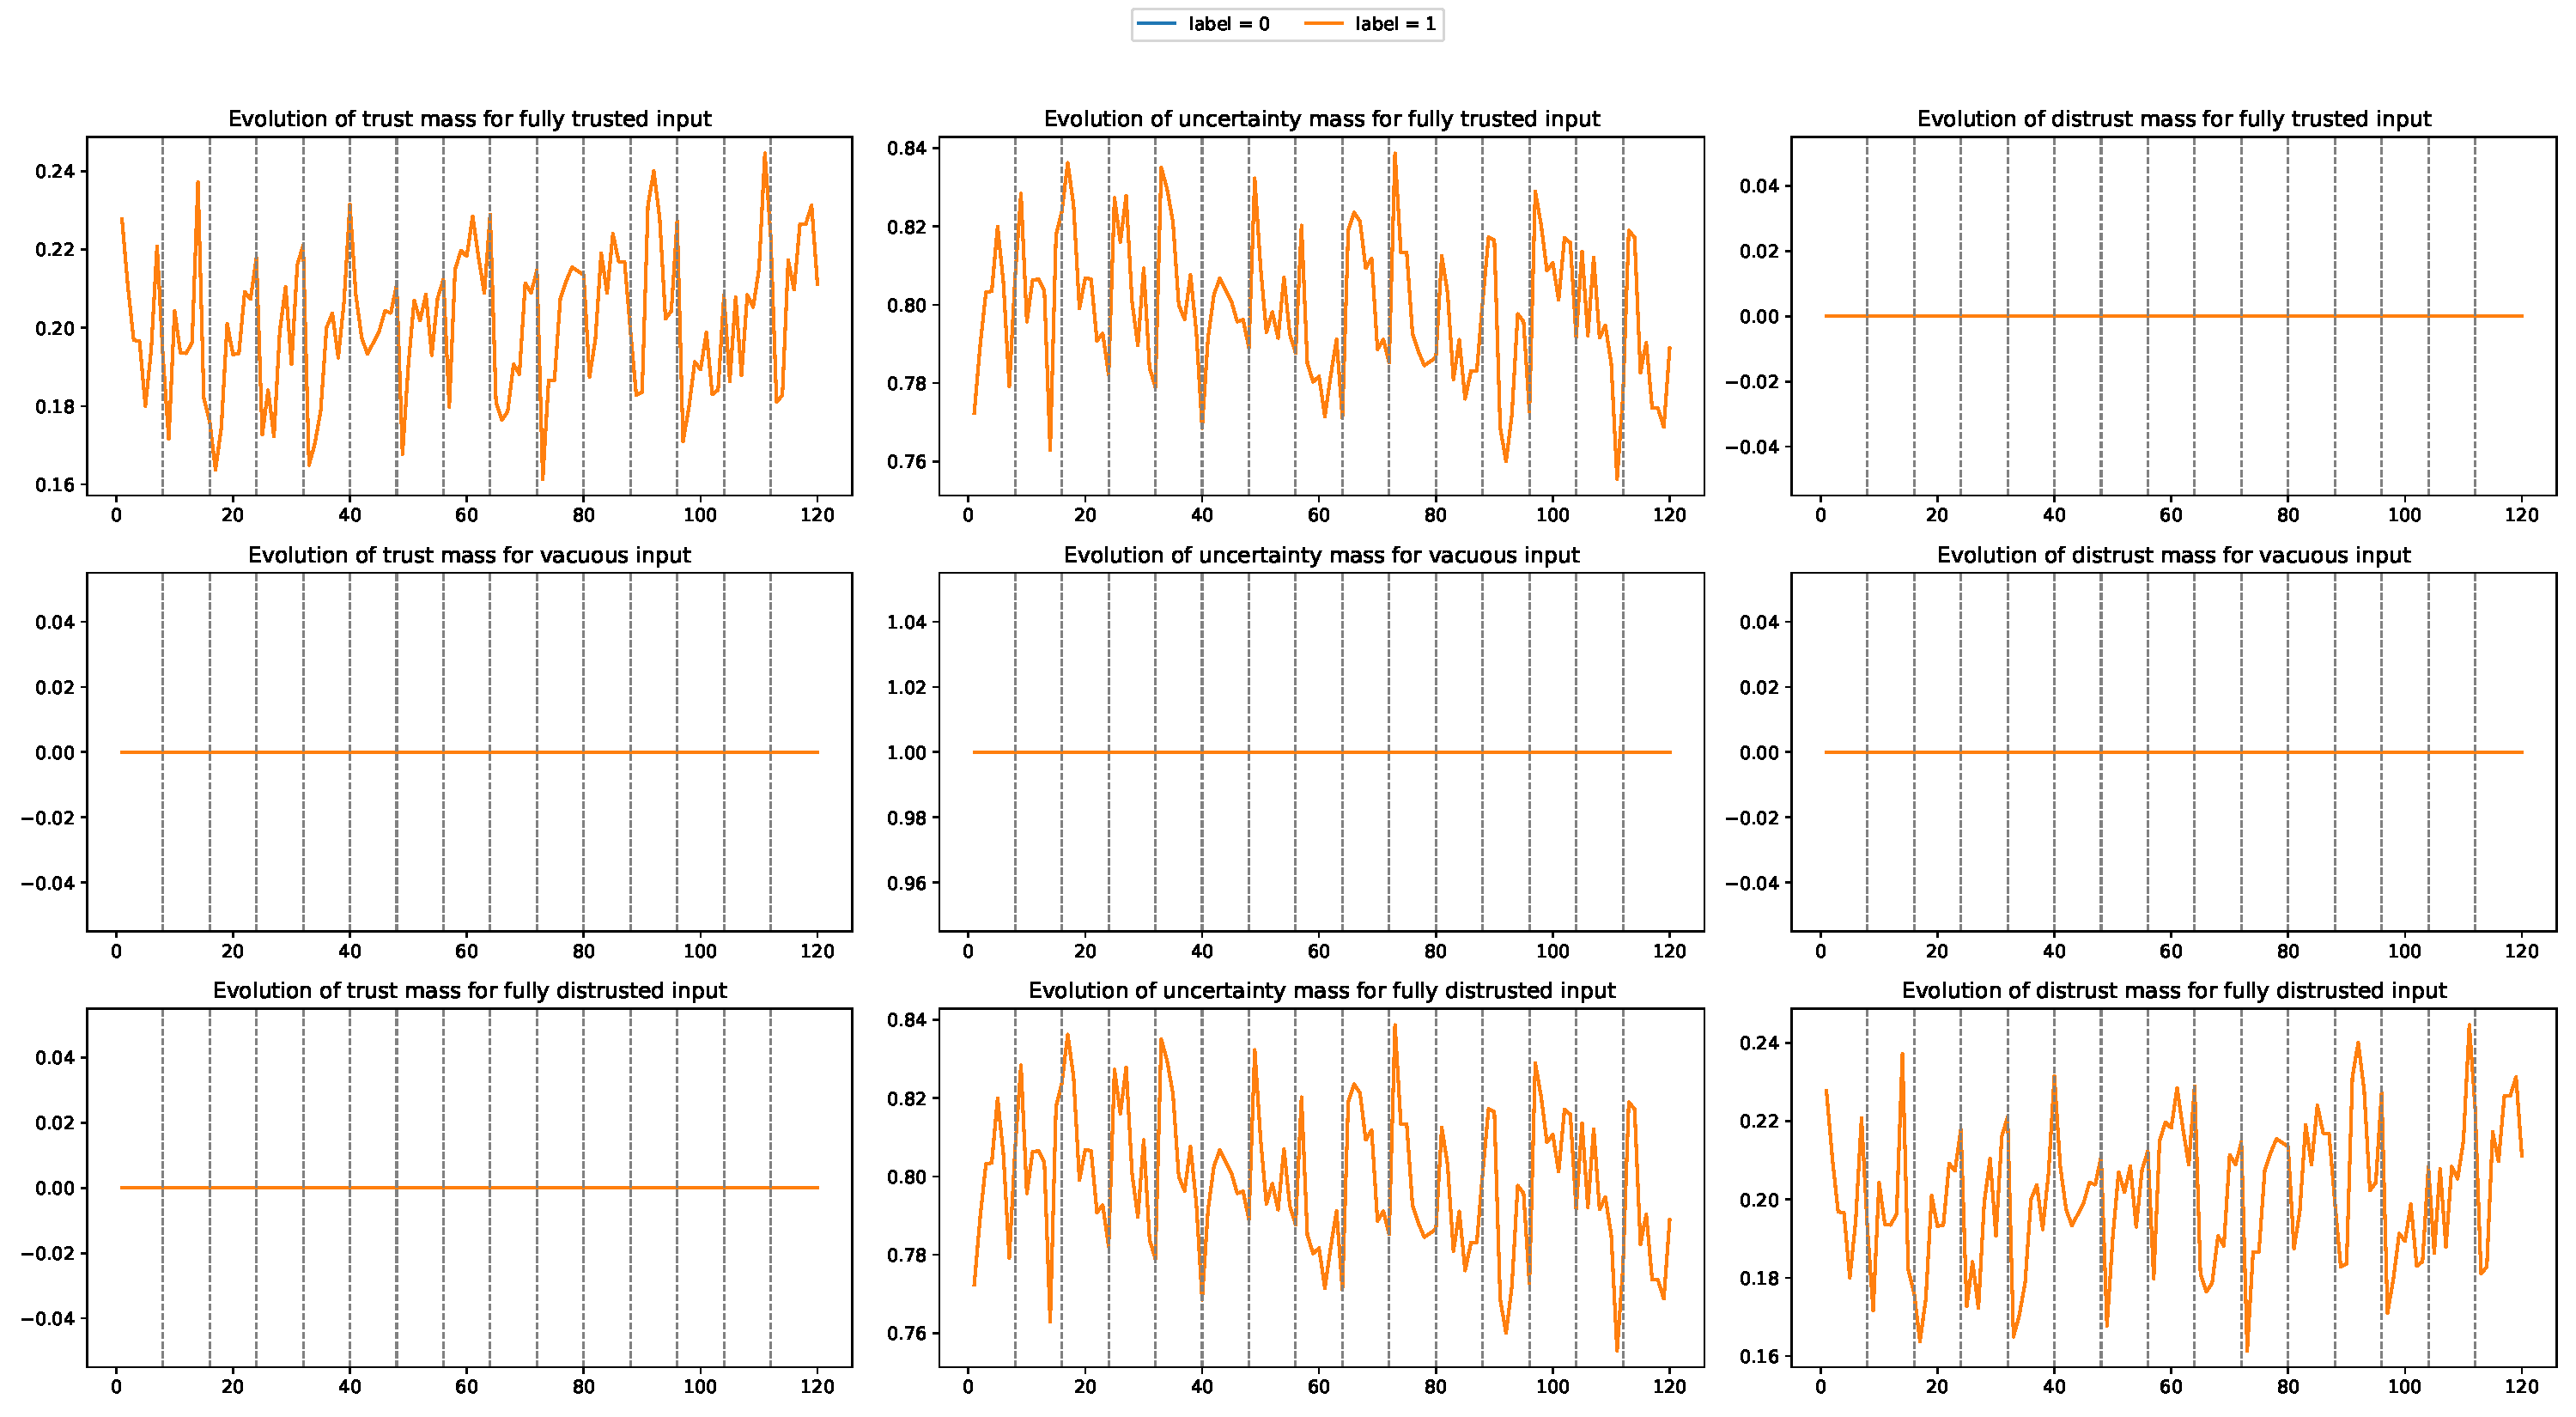
\includegraphics[width=\textwidth]{plots_v2/Cancer/eps=0.01/plot_ptas-v-v.pdf}
  \caption{Features vacuous and labels vacuous}
\end{figure}
\begin{figure}[H]
  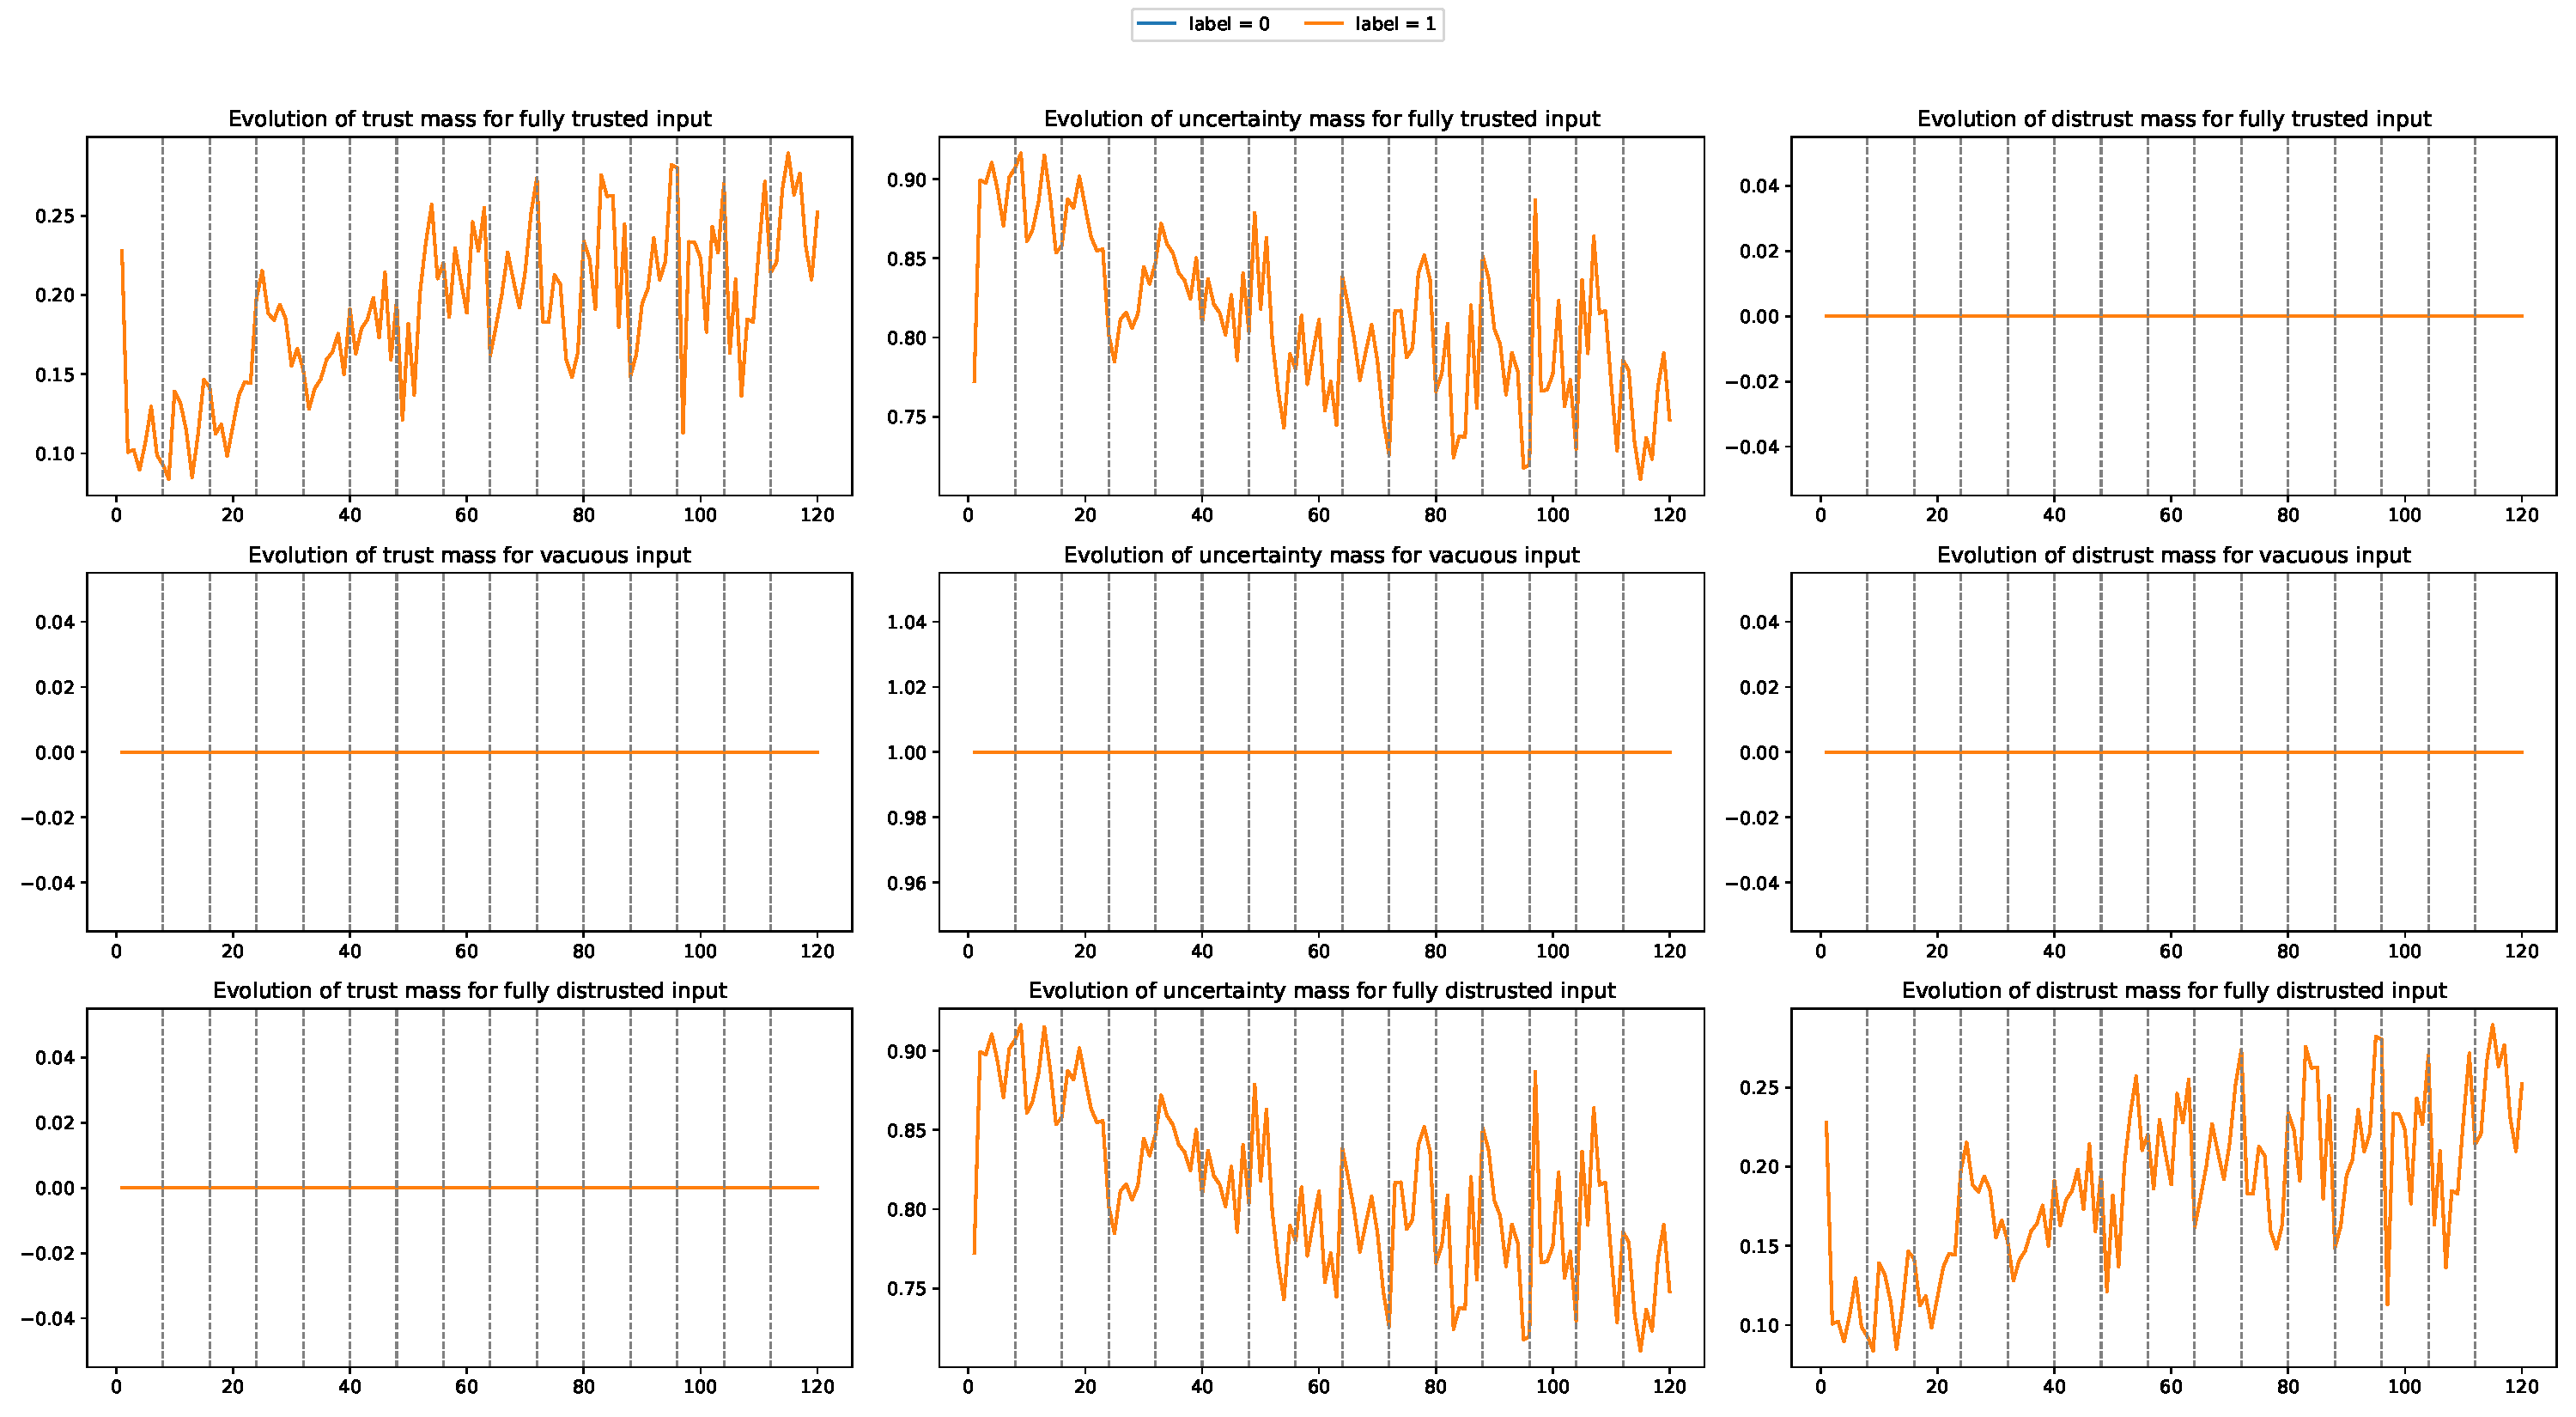
\includegraphics[width=\textwidth]{plots_v2/Cancer/eps=0.01/plot_ptas-v-t.pdf}
  \caption{Features vacuous and labels trusted}
\end{figure}
\begin{figure}[H]
  \includegraphics[width=\textwidth]{plots_v2/Cancer/eps=0.01/plot_ptas-t-d.pdf}
  \caption{Features trusted and labels distrusted}
\end{figure}
\begin{figure}[H]
  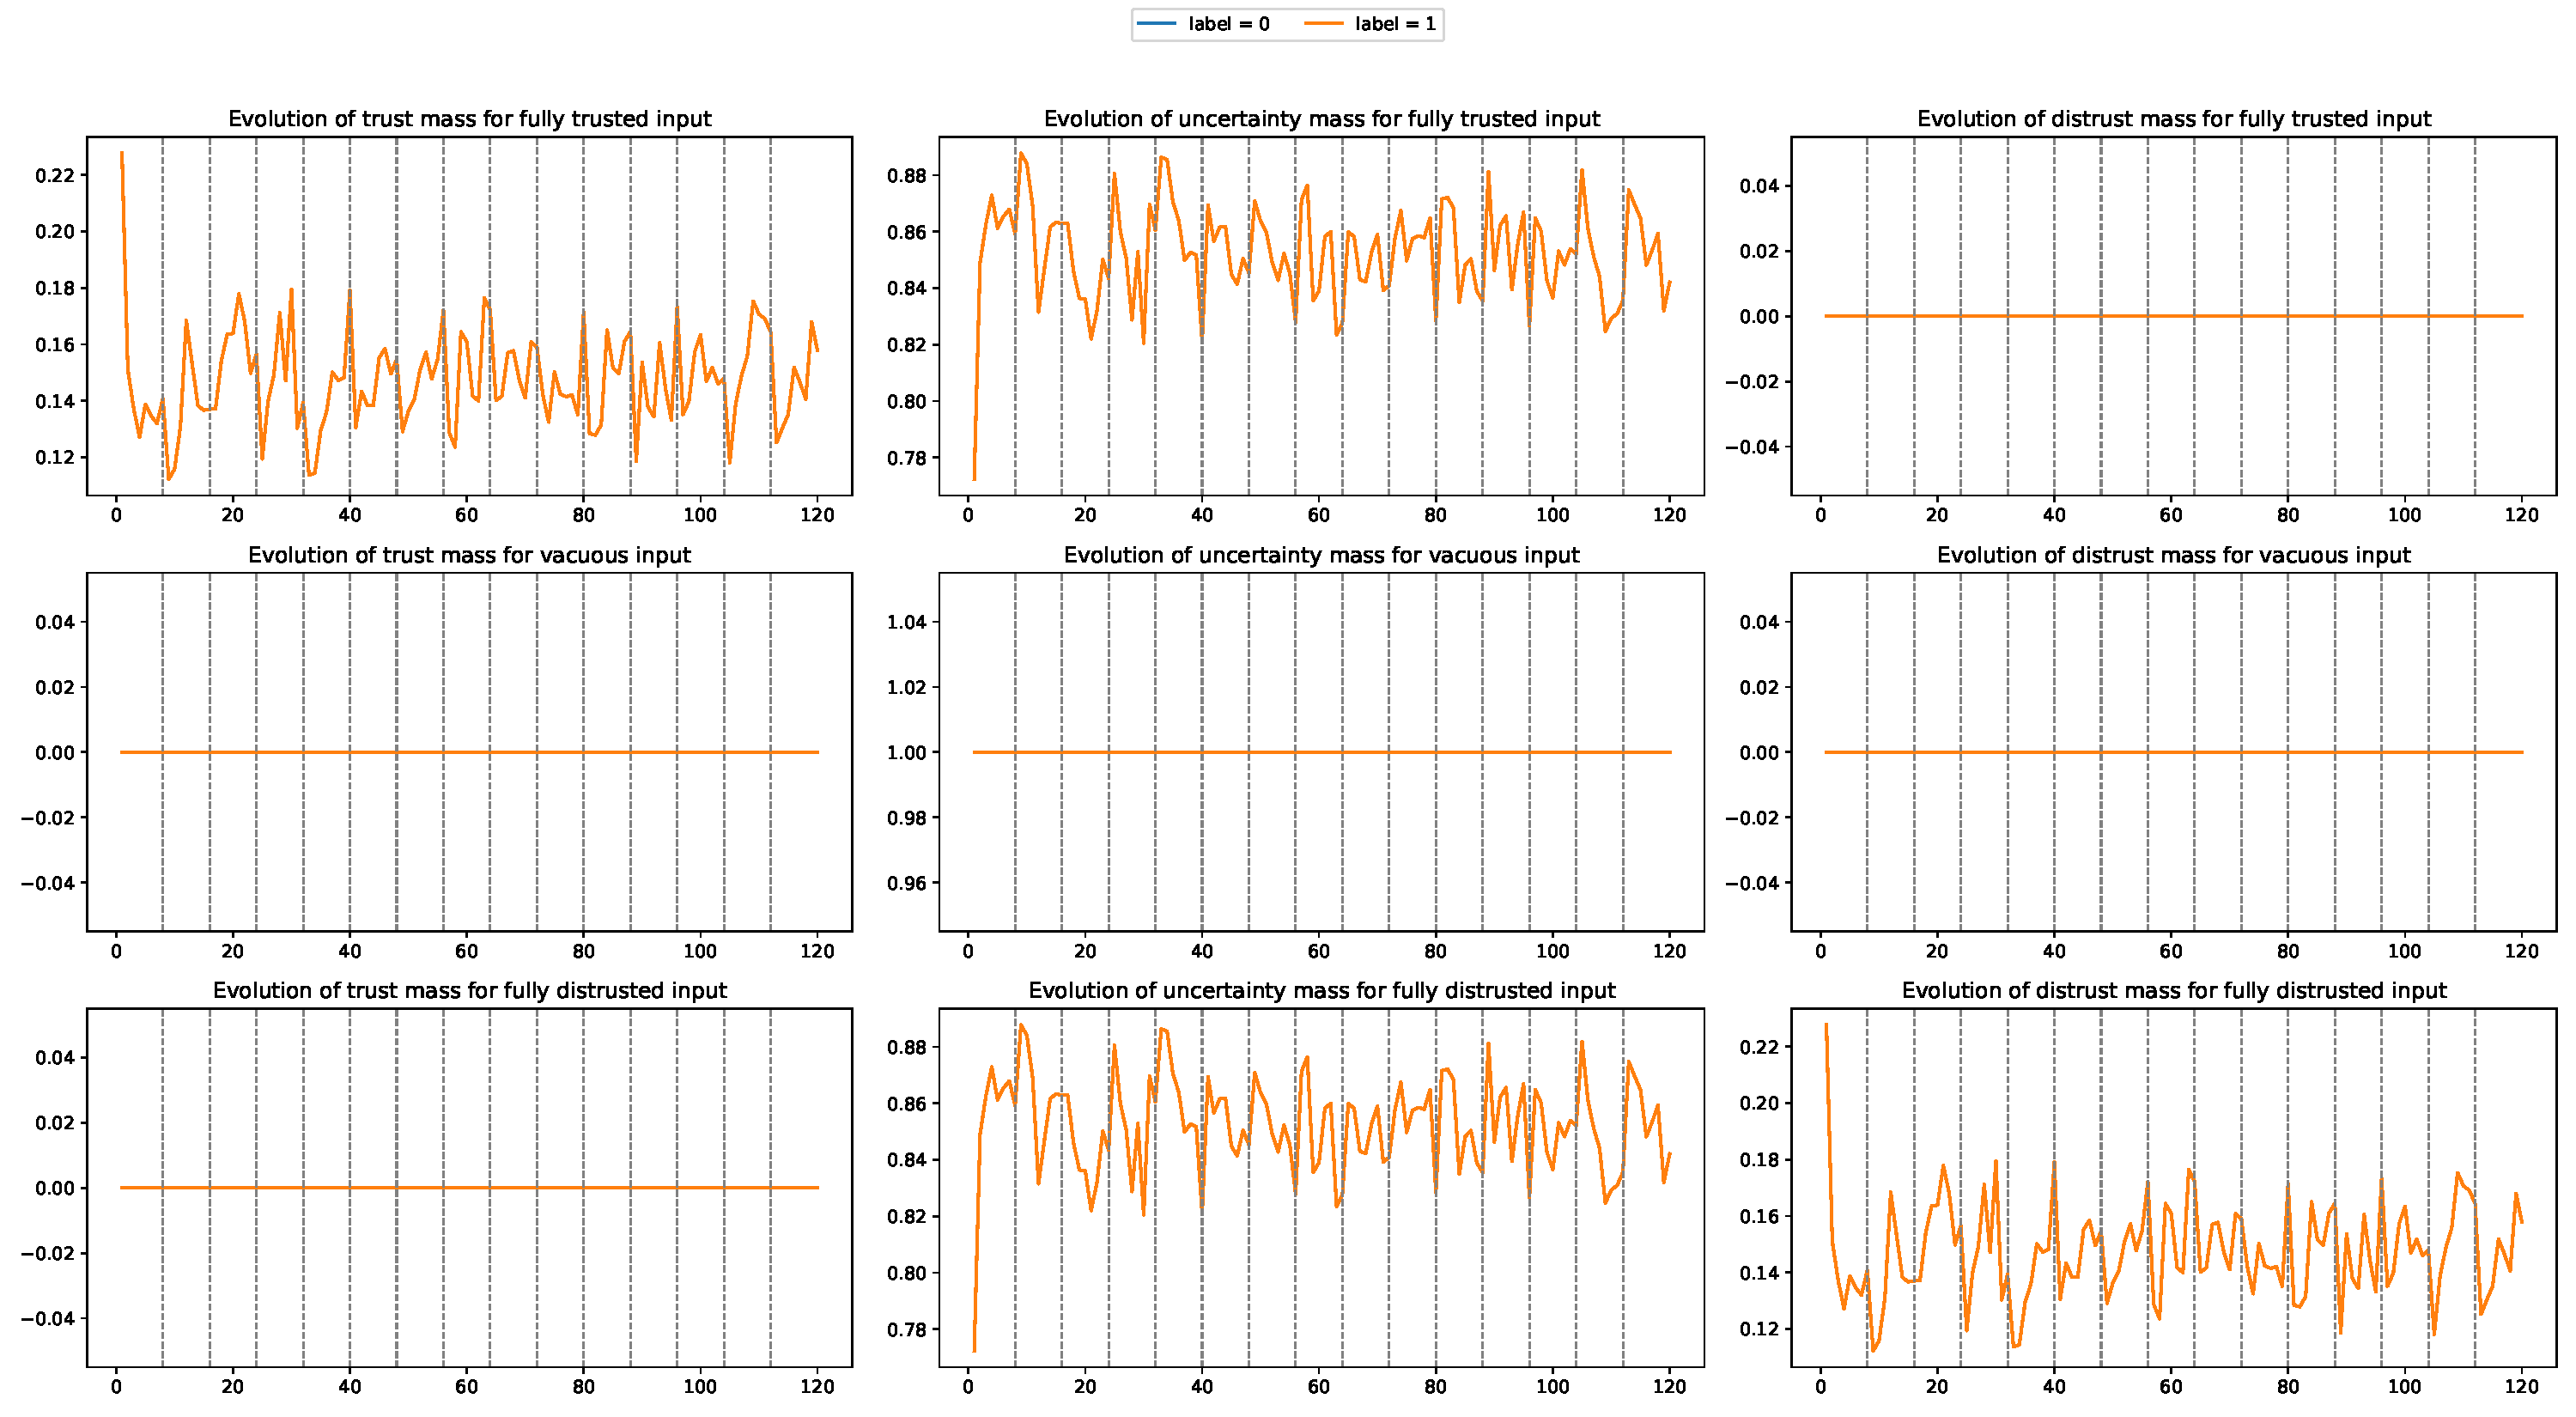
\includegraphics[width=\textwidth]{plots_v2/Cancer/eps=0.01/plot_ptas-t-v.pdf}
  \caption{Features trusted and labels vacuous}
\end{figure}
\begin{figure}[H]
  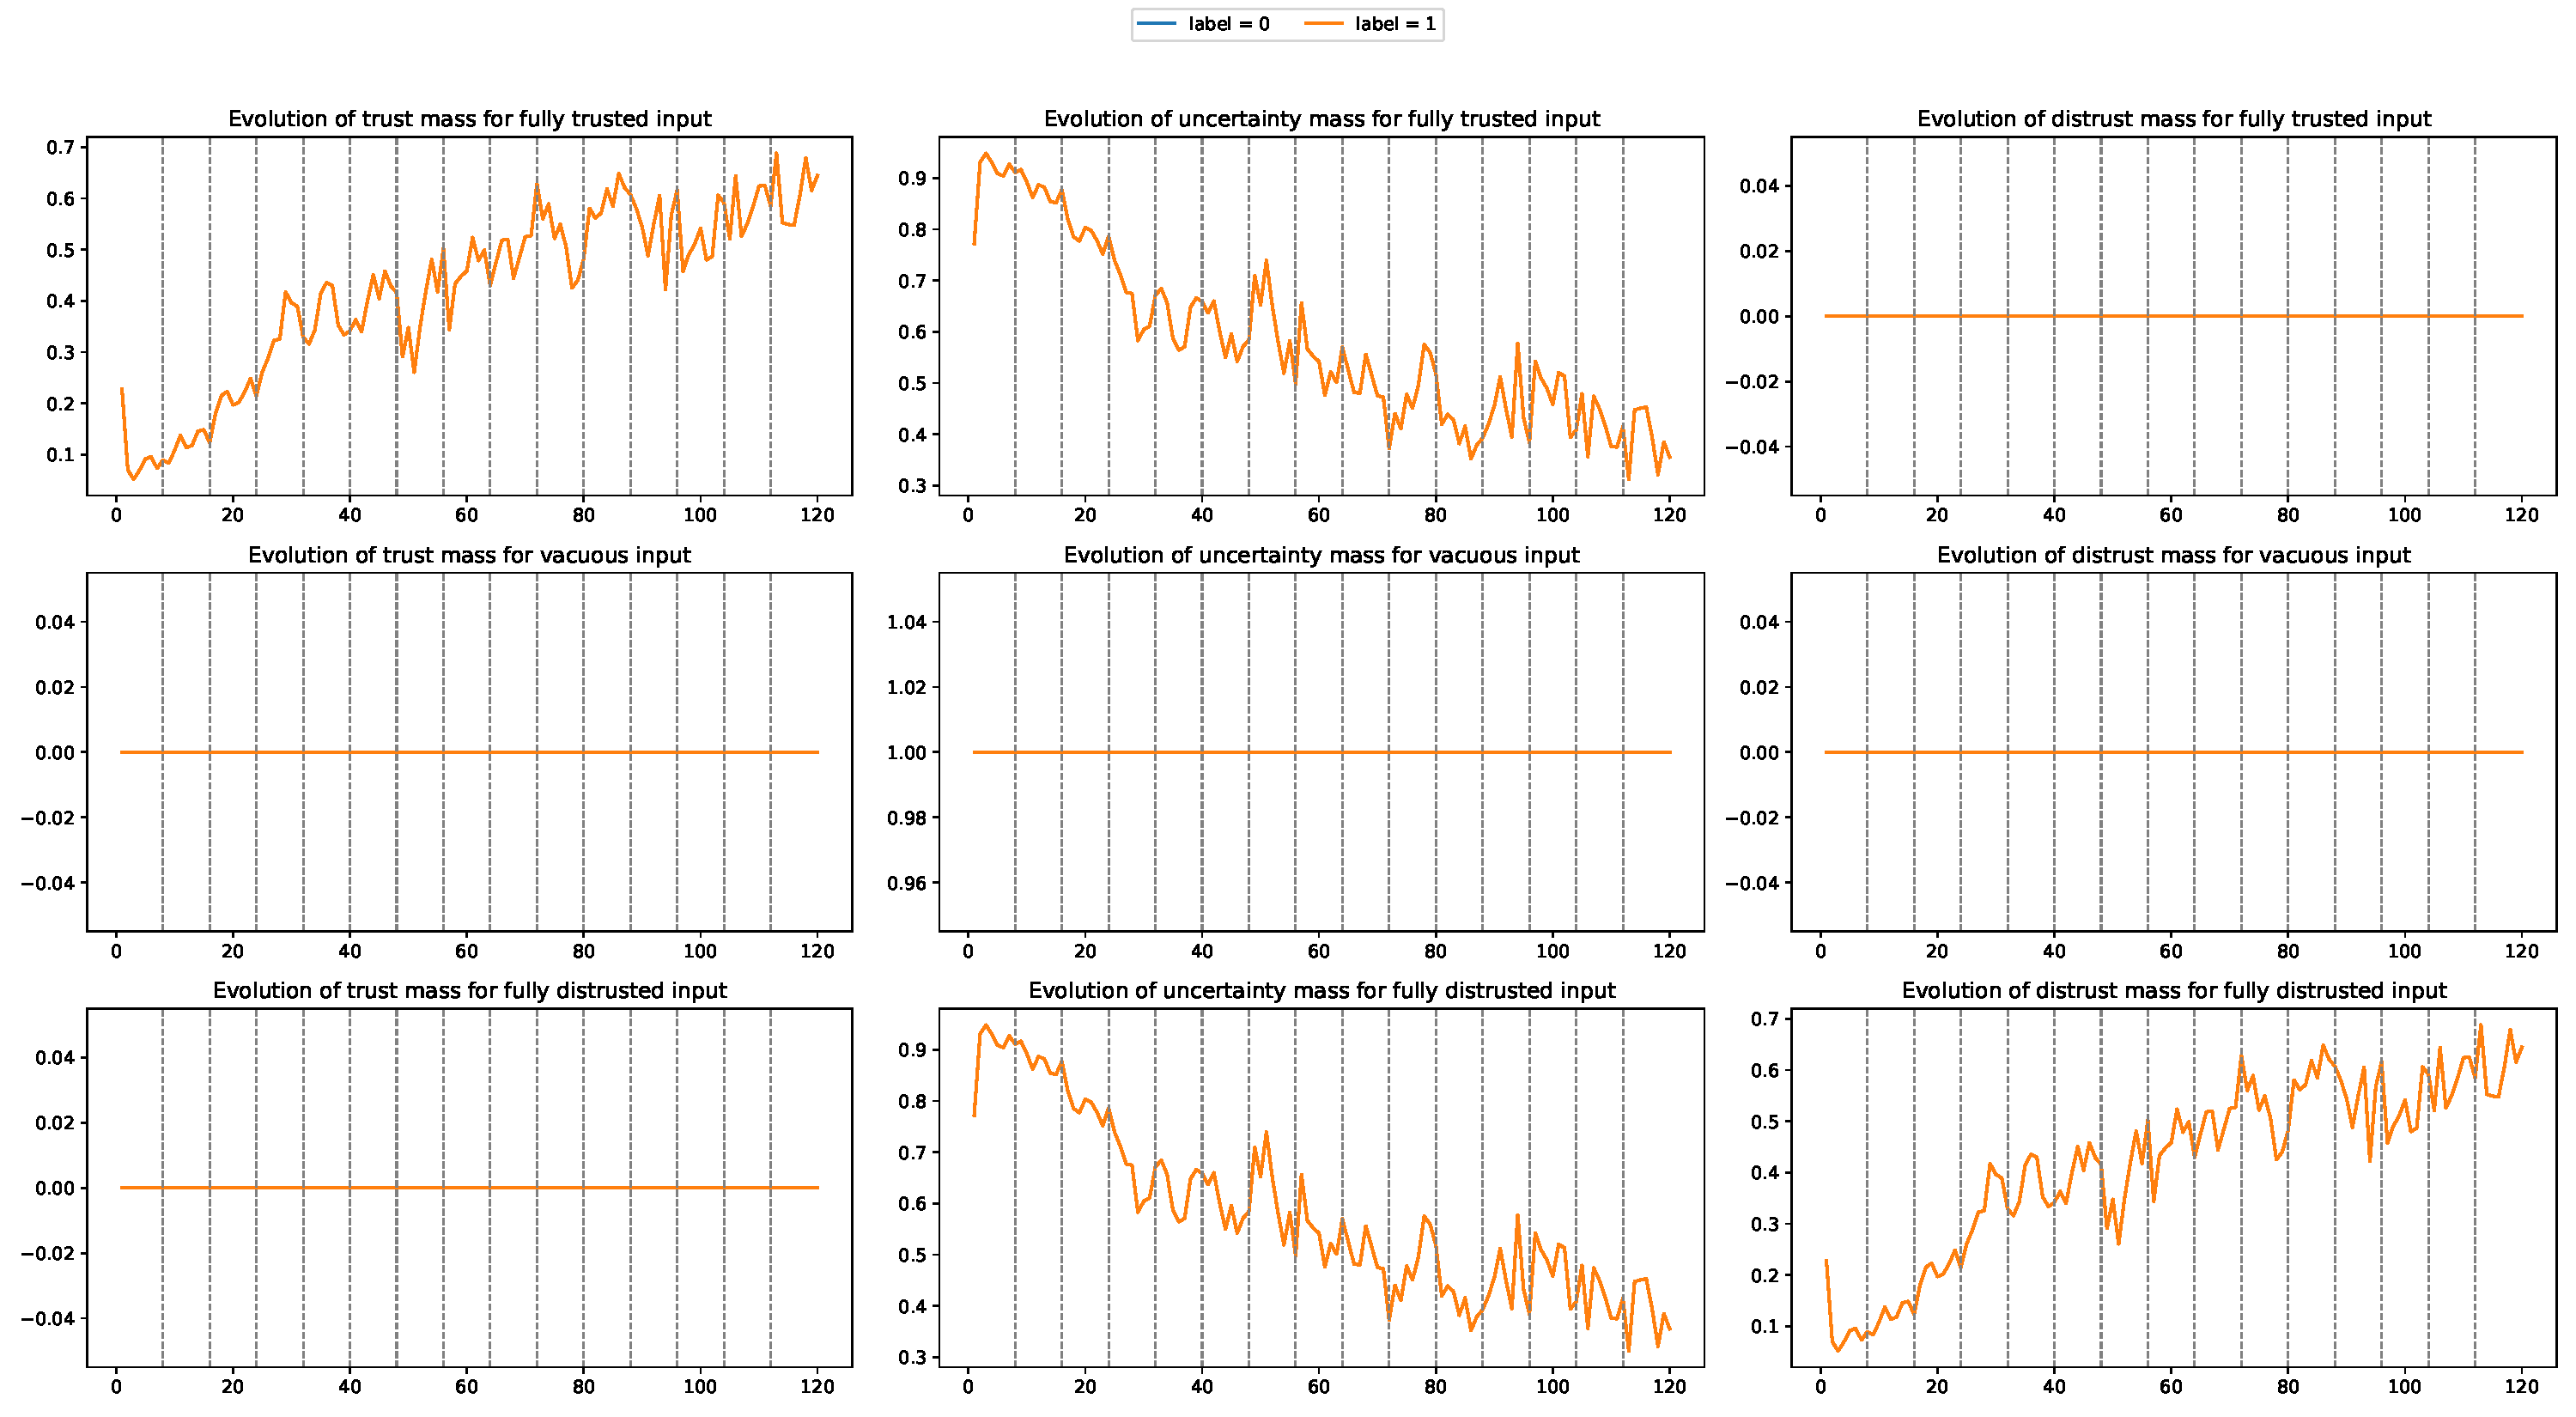
\includegraphics[width=\textwidth]{plots_v2/Cancer/eps=0.01/plot_ptas-t-t.pdf}
  \caption{Features trusted and labels trusted}
\end{figure}

\subsection{Cancer Model with \( \epsilon = 0.1 \)(\cref{exp:1})}\label{sec:rescancer0.1}
\begin{figure}[H]
  \includegraphics[width=\textwidth]{plots_v2/Cancer/eps=0.1/plot_ptas-d-d.pdf}
  \caption{Features distrusted and labels distrusted}
\end{figure}
\begin{figure}[H]
  \includegraphics[width=\textwidth]{plots_v2/Cancer/eps=0.1/plot_ptas-d-v.pdf}
  \caption{Features distrusted and labels vacuous}
\end{figure}
\begin{figure}[H]
  \includegraphics[width=\textwidth]{plots_v2/Cancer/eps=0.1/plot_ptas-d-t.pdf}
  \caption{Features distrusted and labels trusted}
\end{figure}
\begin{figure}[H]
  \includegraphics[width=\textwidth]{plots_v2/Cancer/eps=0.1/plot_ptas-v-d.pdf}
  \caption{Features vacuous and labels distrusted}
\end{figure}
\begin{figure}[H]
  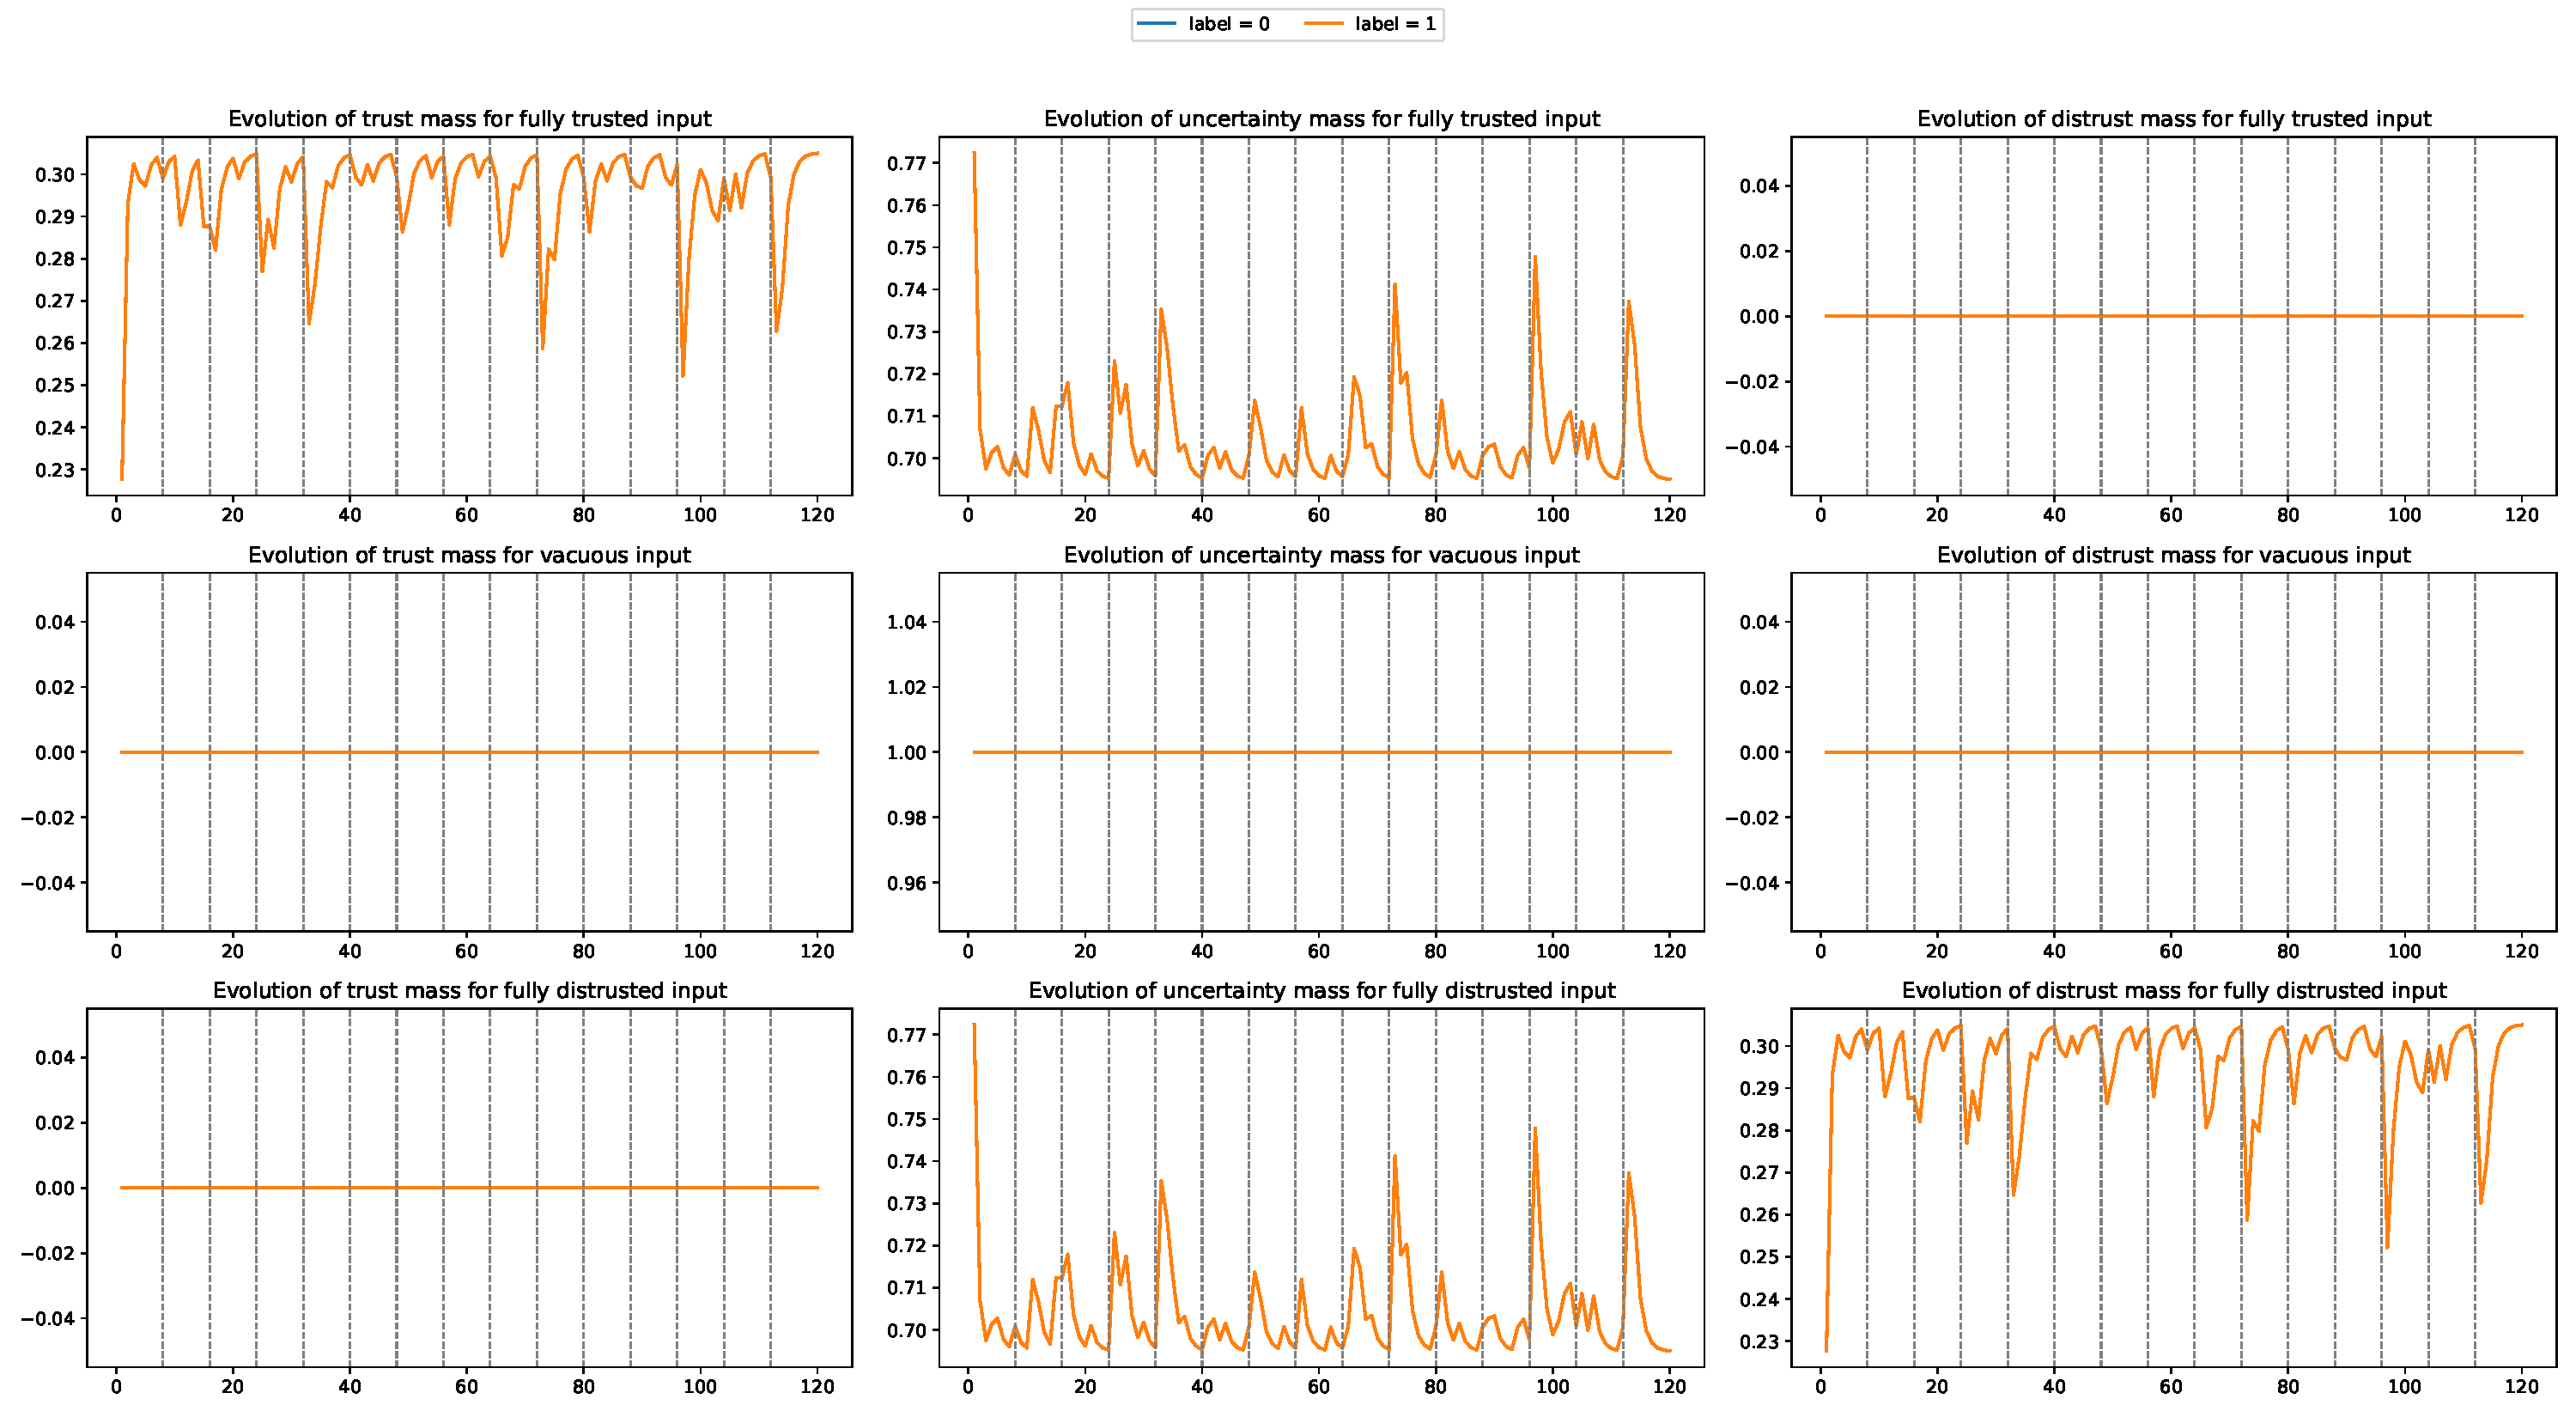
\includegraphics[width=\textwidth]{plots_v2/Cancer/eps=0.1/plot_ptas-v-v.pdf}
  \caption{Features vacuous and labels vacuous}
\end{figure}
\begin{figure}[H]
  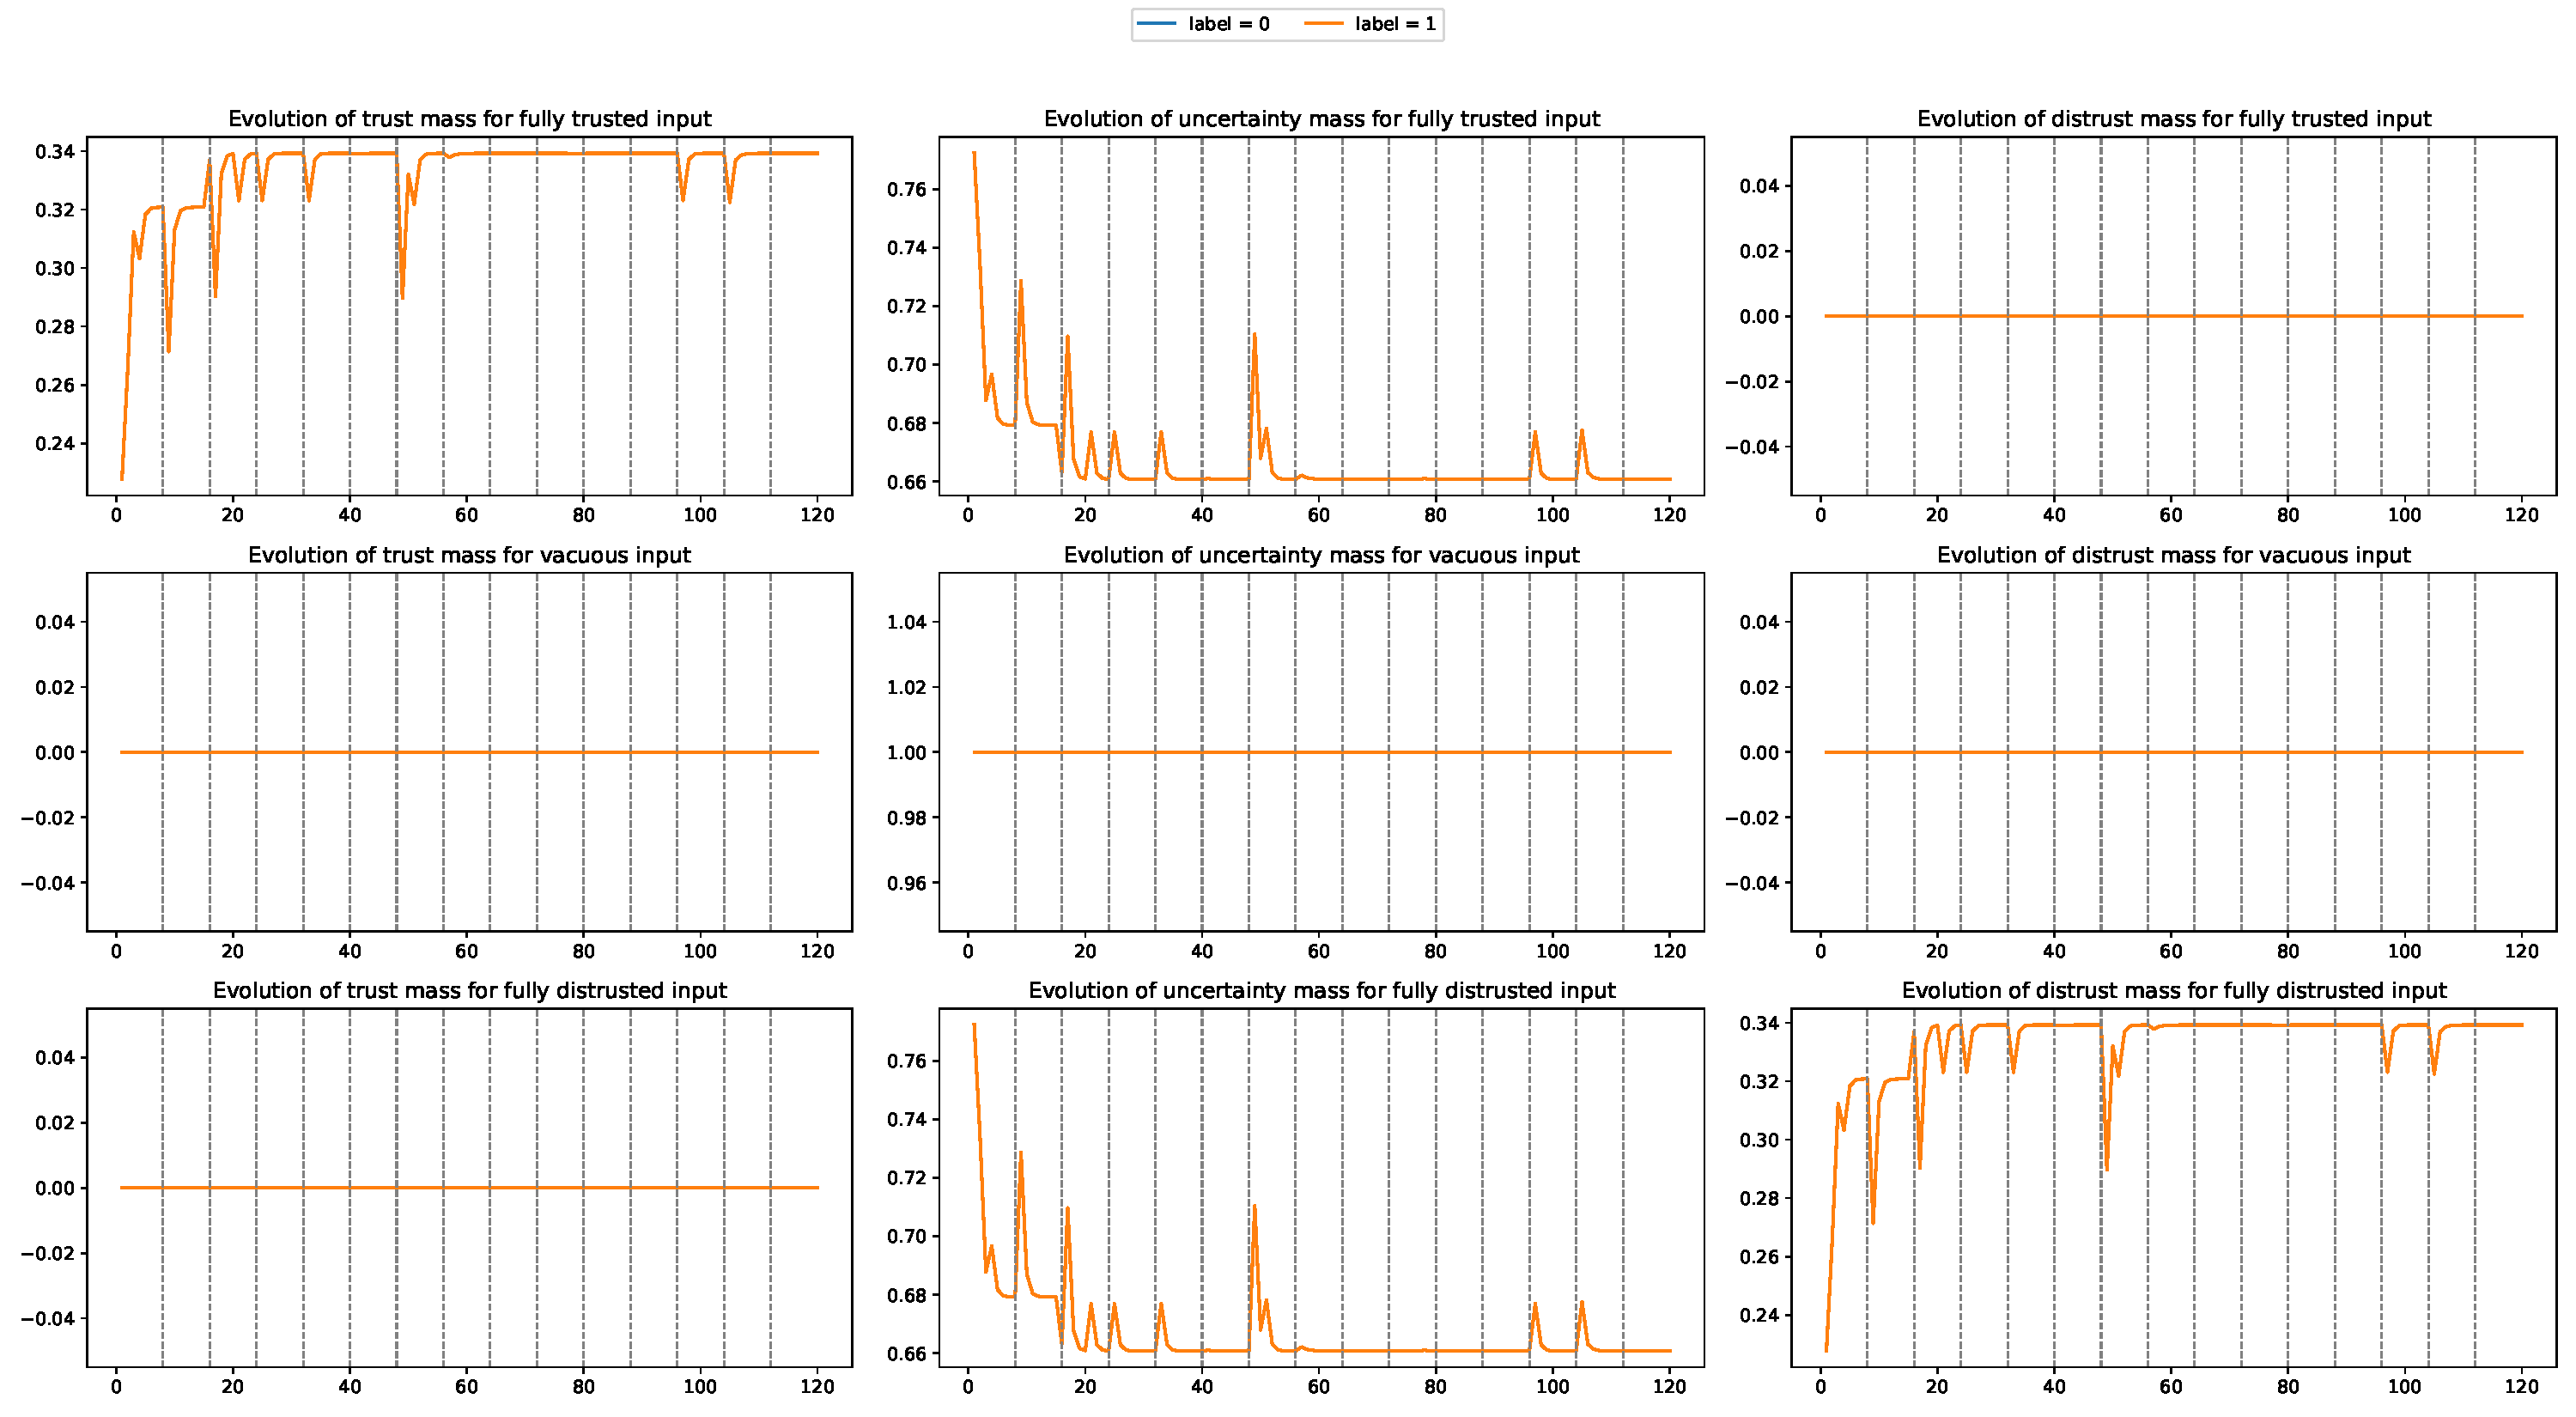
\includegraphics[width=\textwidth]{plots_v2/Cancer/eps=0.1/plot_ptas-v-t.pdf}
  \caption{Features vacuous and labels trusted}
\end{figure}
\begin{figure}[H]
  \includegraphics[width=\textwidth]{plots_v2/Cancer/eps=0.1/plot_ptas-t-d.pdf}
  \caption{Features trusted and labels distrusted}
\end{figure}
\begin{figure}[H]
  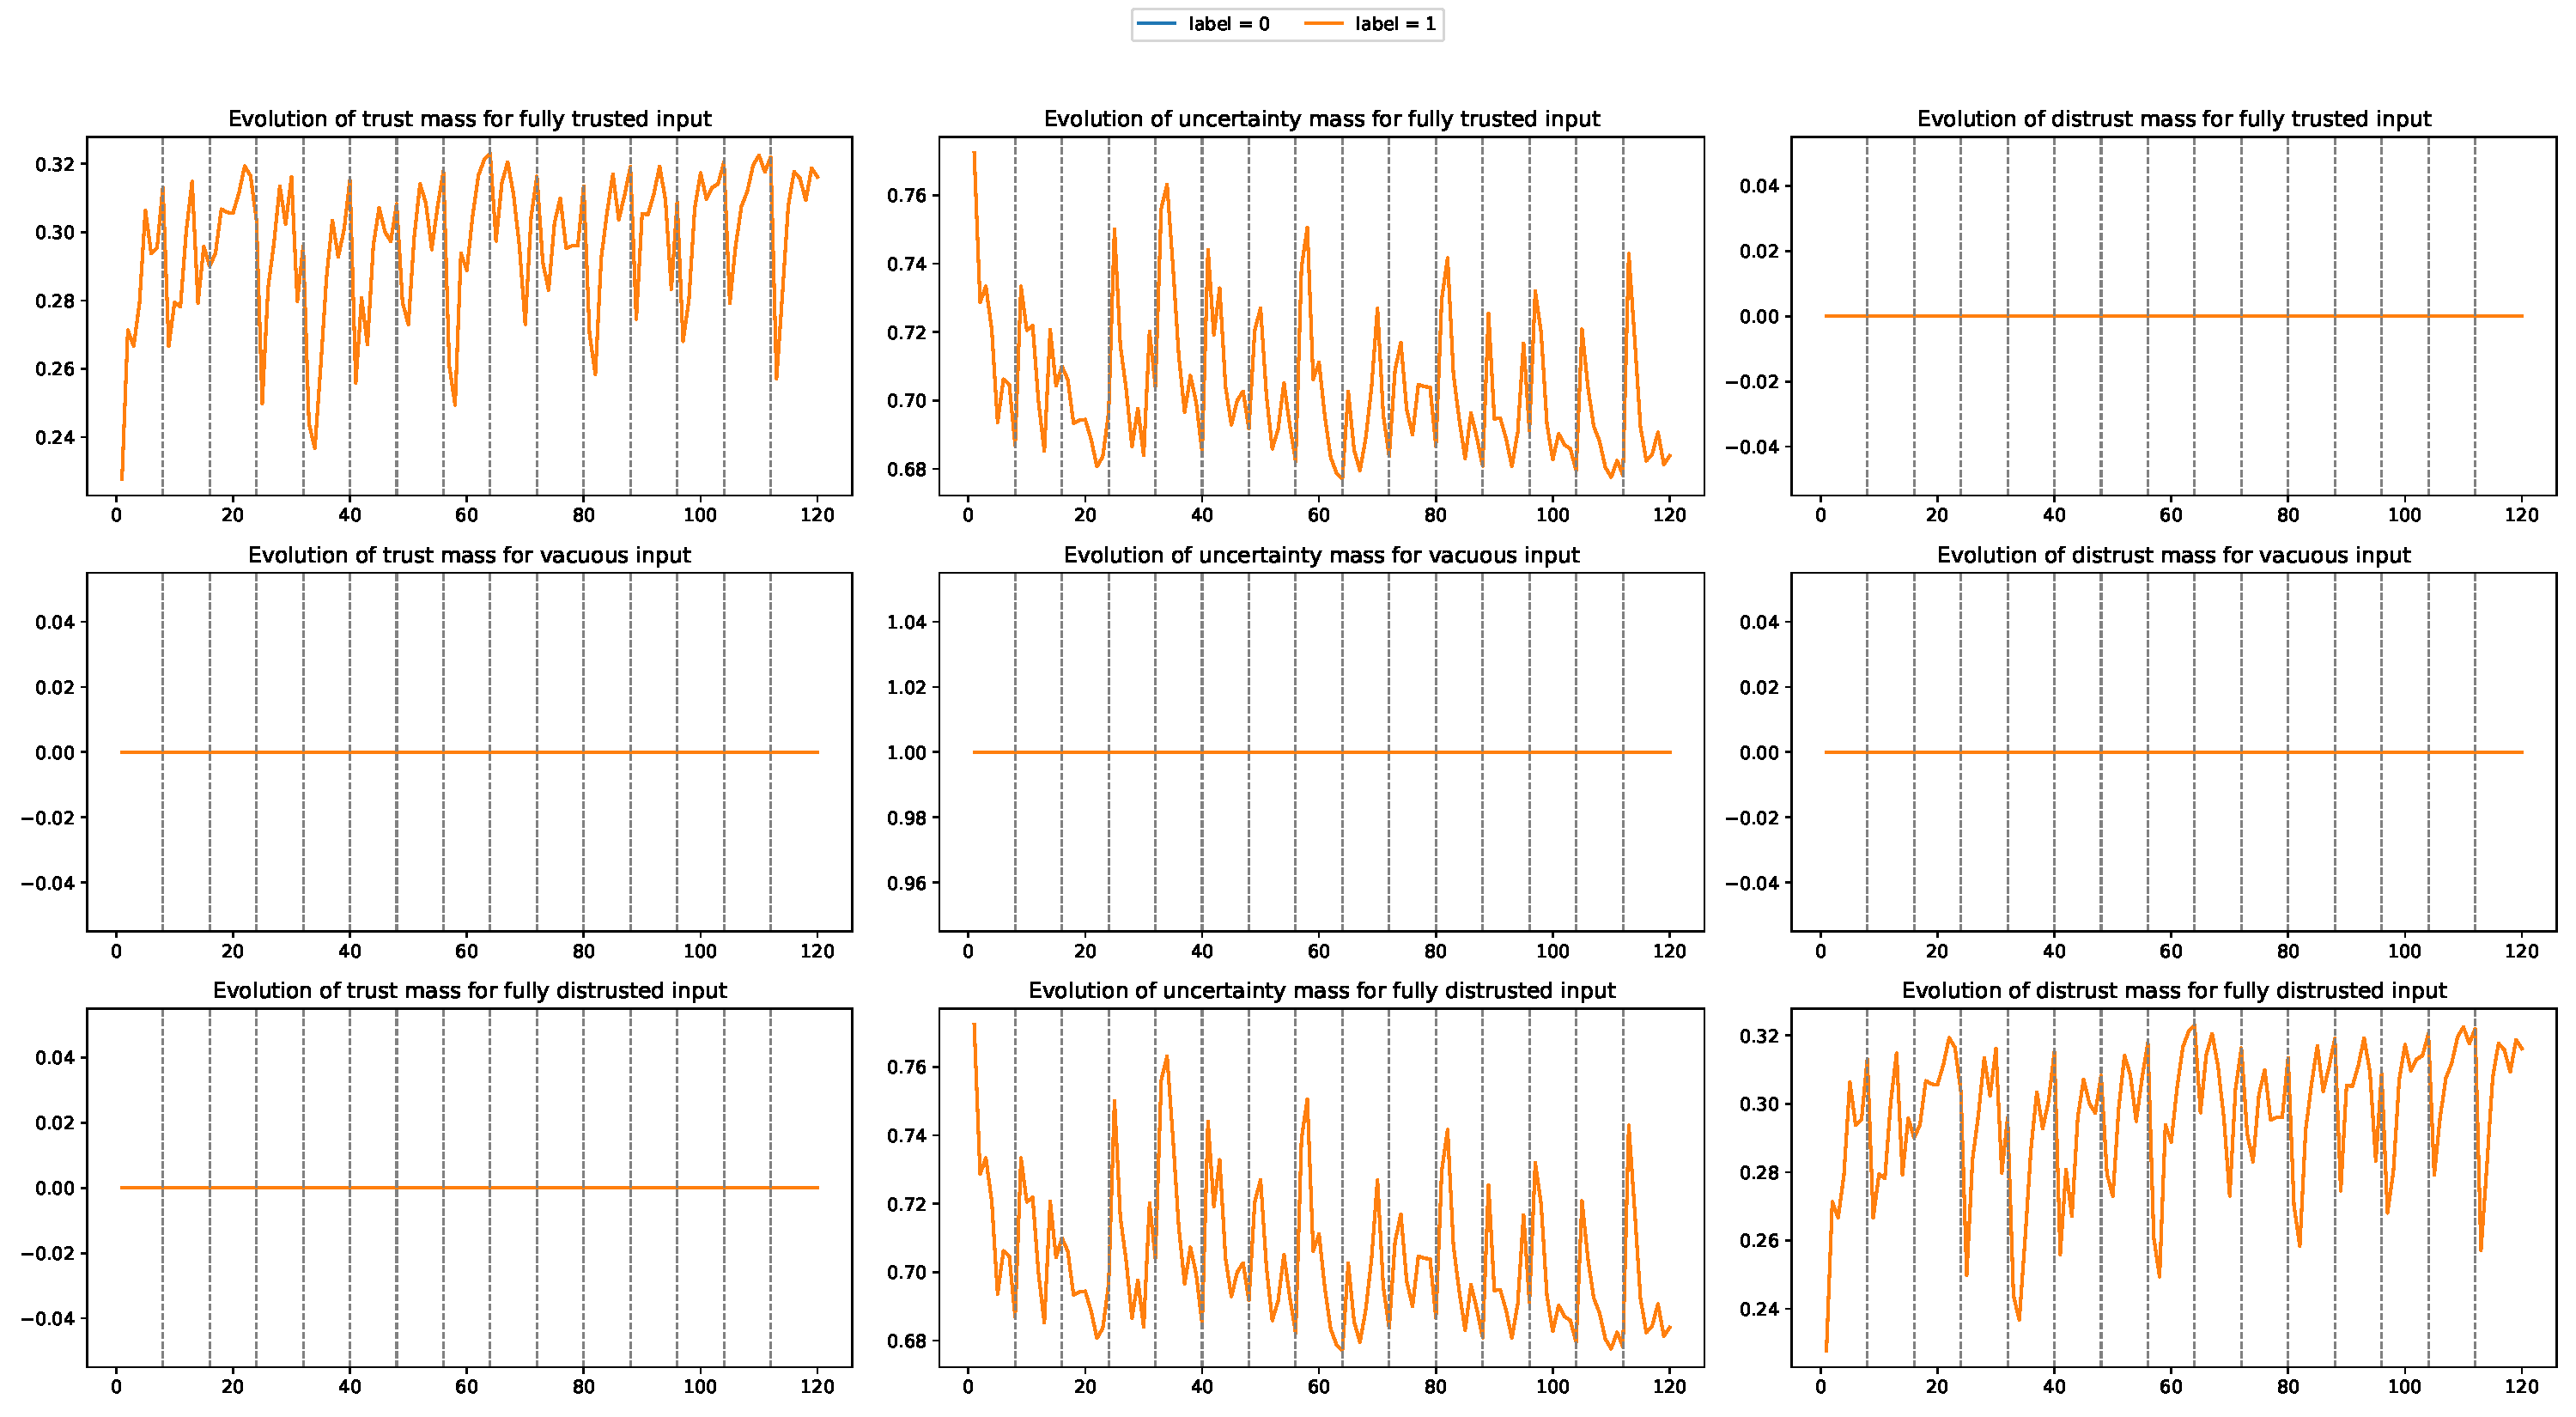
\includegraphics[width=\textwidth]{plots_v2/Cancer/eps=0.1/plot_ptas-t-v.pdf}
  \caption{Features trusted and labels vacuous}
\end{figure}
\begin{figure}[H]
  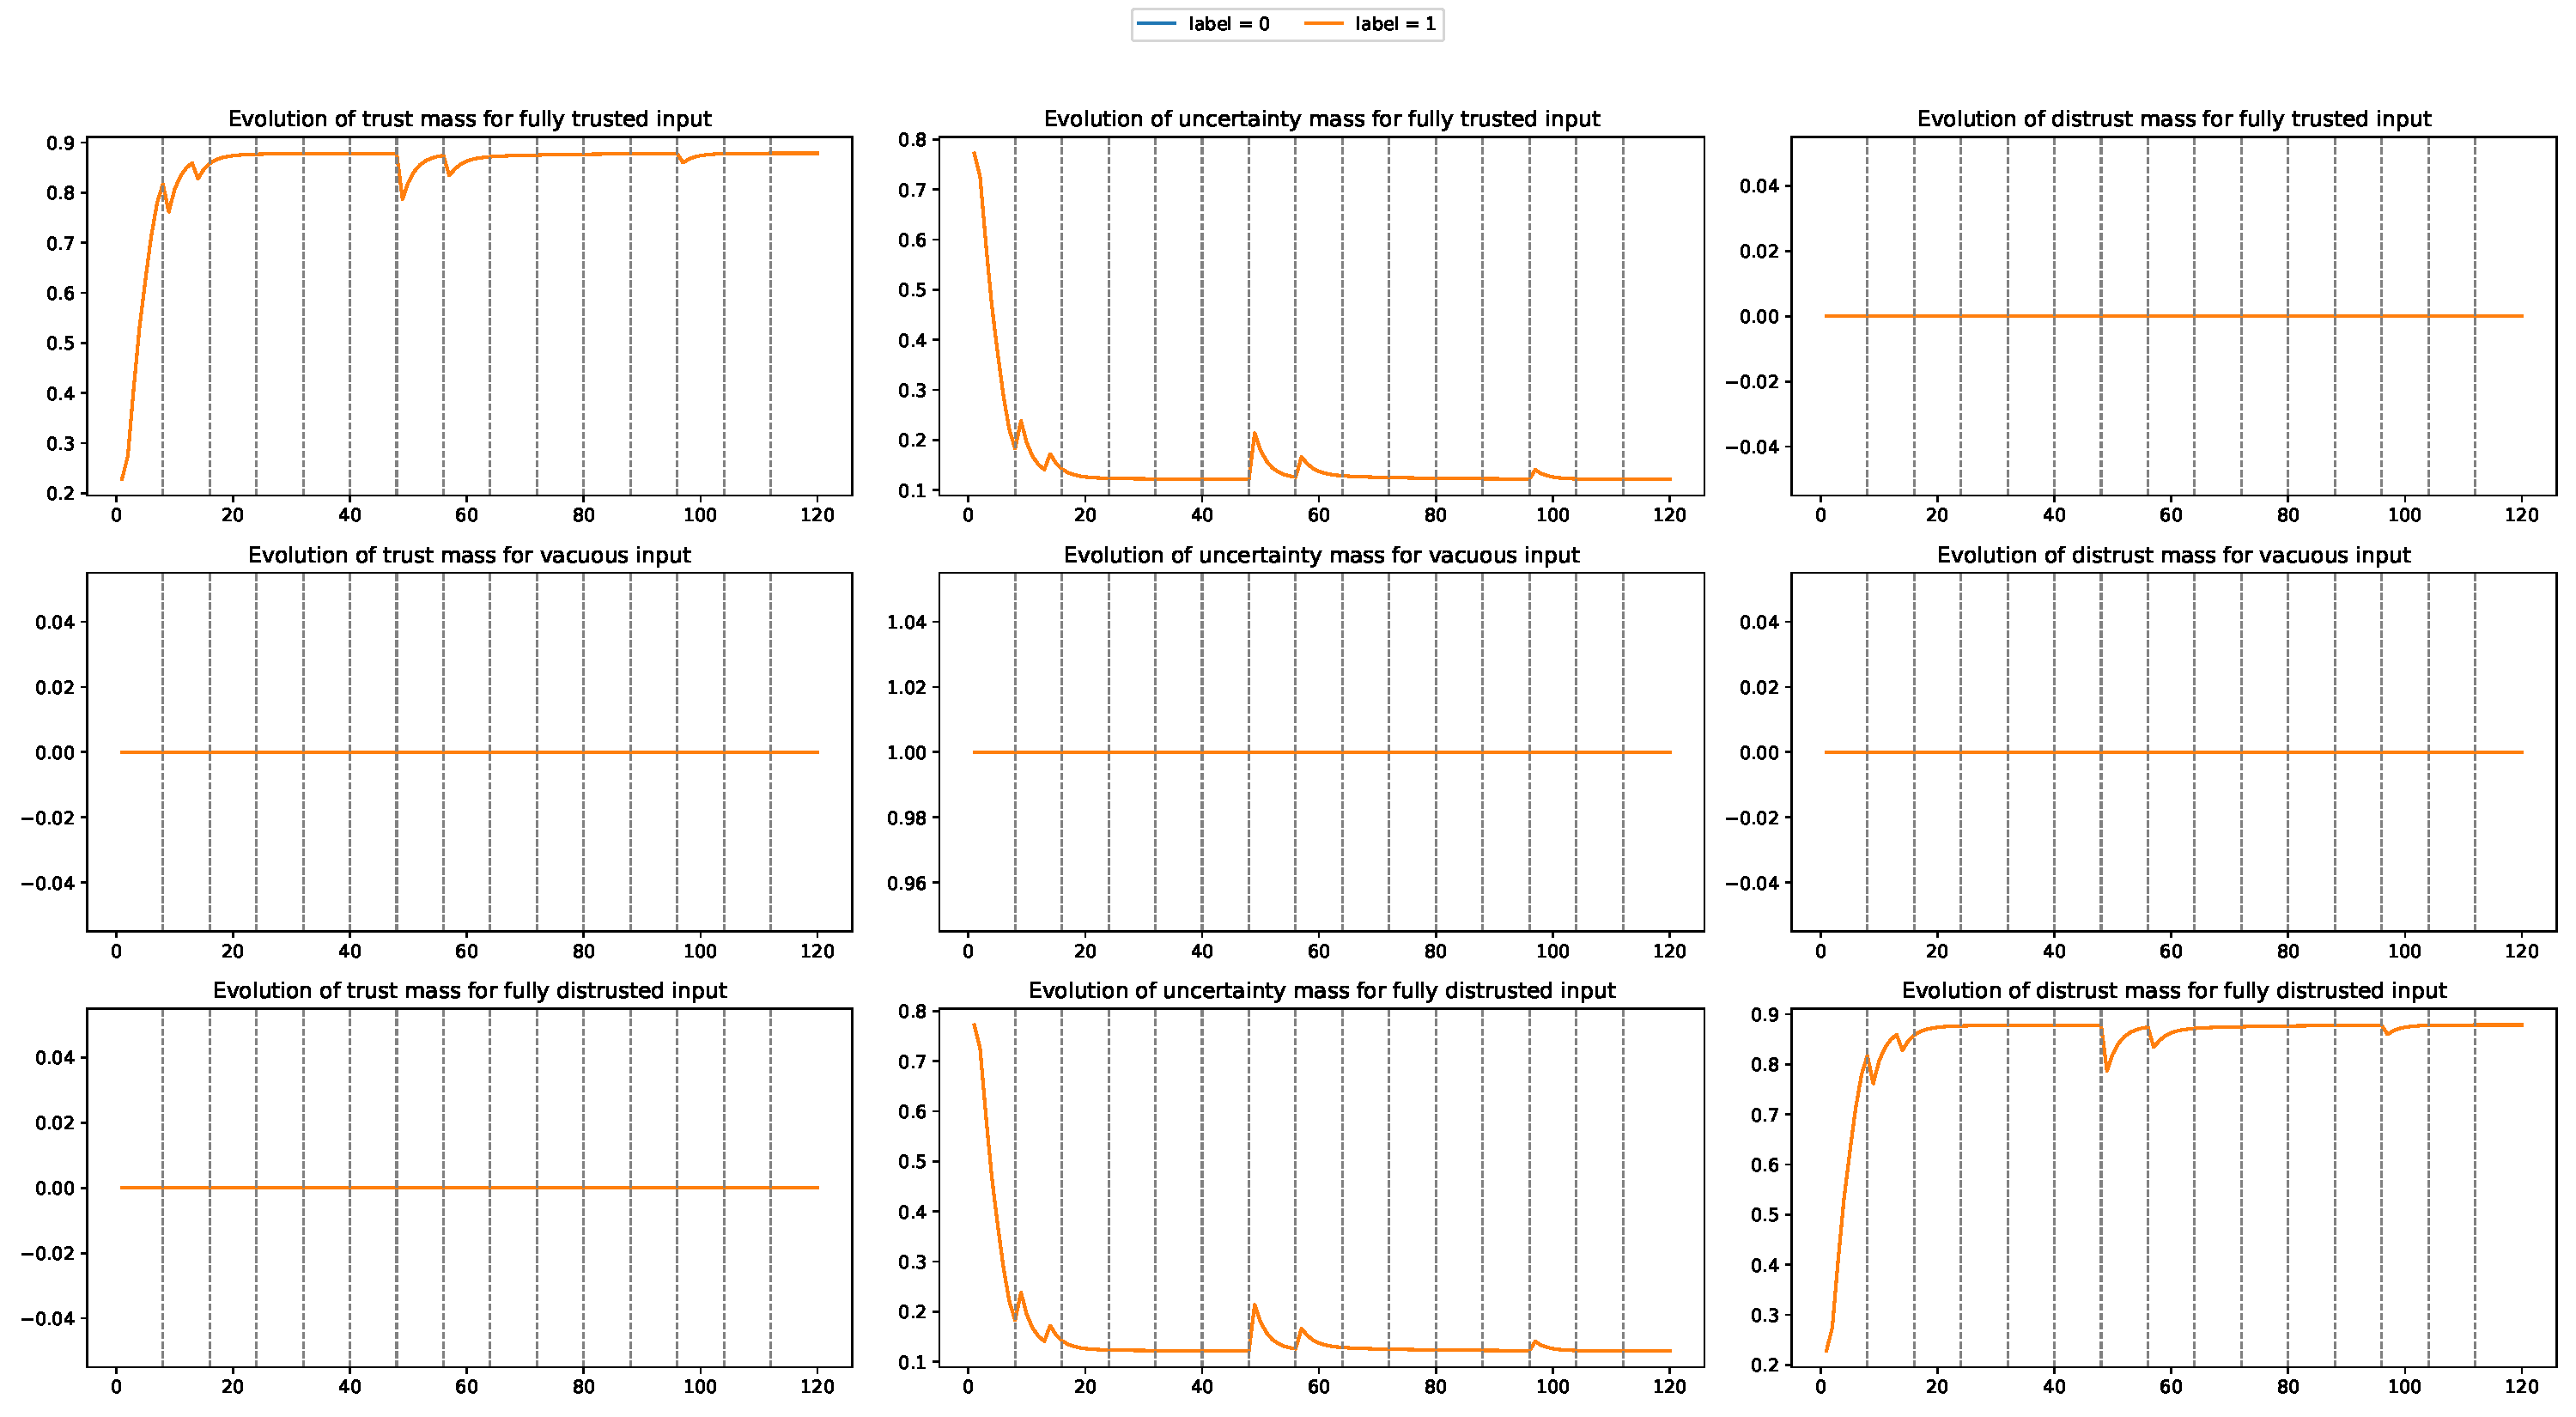
\includegraphics[width=\textwidth]{plots_v2/Cancer/eps=0.1/plot_ptas-t-t.pdf}
  \caption{Features trusted and labels trusted}
\end{figure}

\subsection{Accuracy Evolution for the Cancer Model (\cref{exp:1})}\label{sec:resmnistaccapp}
\begin{figure}[H]
\centering
\begin{subfigure}[b]{0.32\textwidth}
  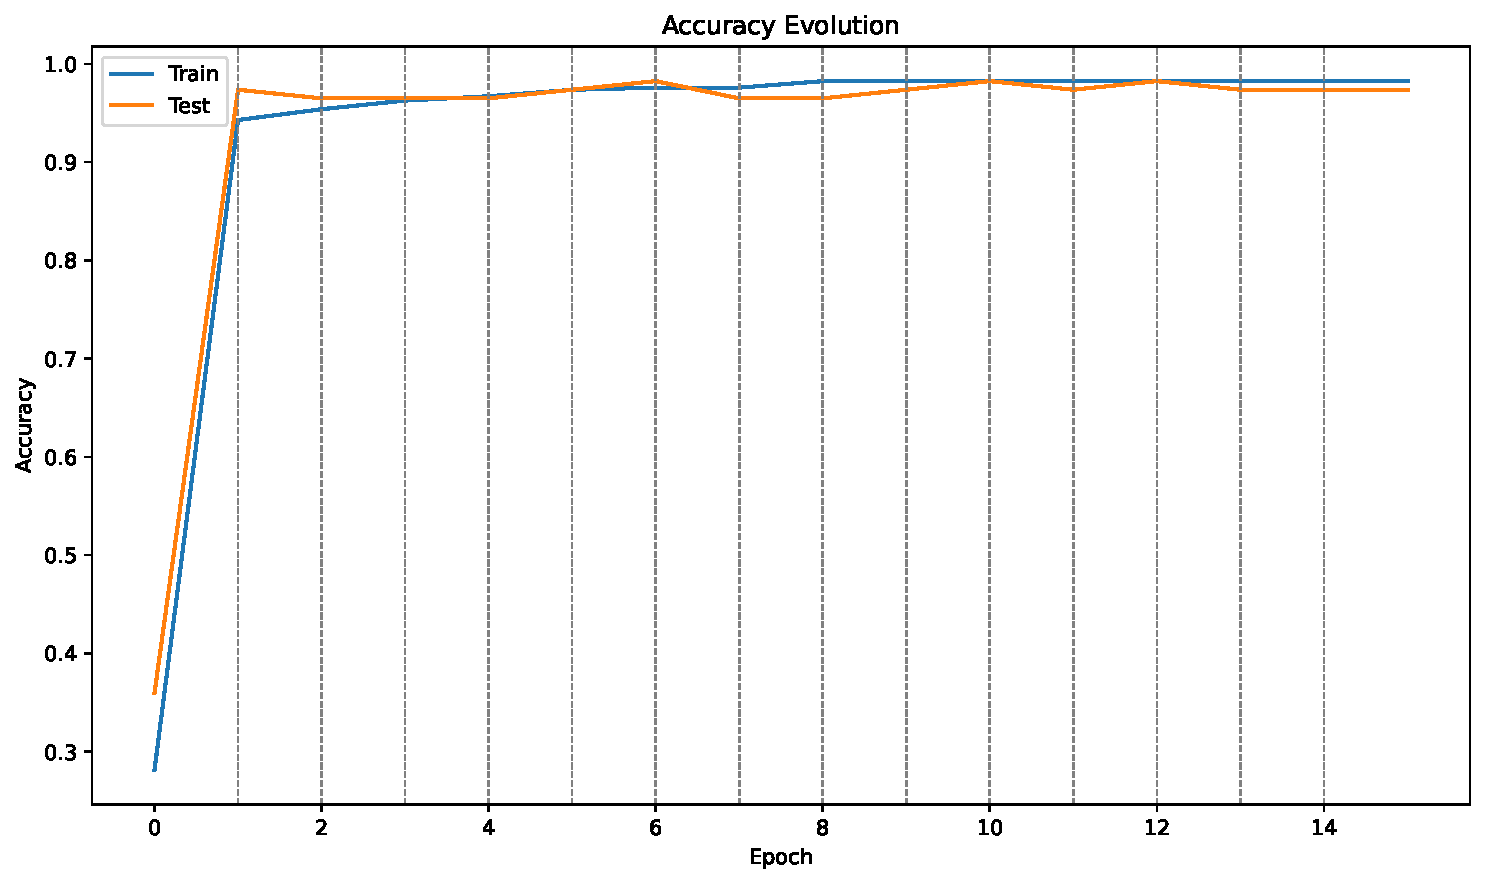
\includegraphics[width=\textwidth]{plots_v2/Cancer/eps=0.1/accuracy_evolution-t-t.pdf}
  \caption{Clean Features and Labels}
\end{subfigure}
\begin{subfigure}[b]{0.32\textwidth}
  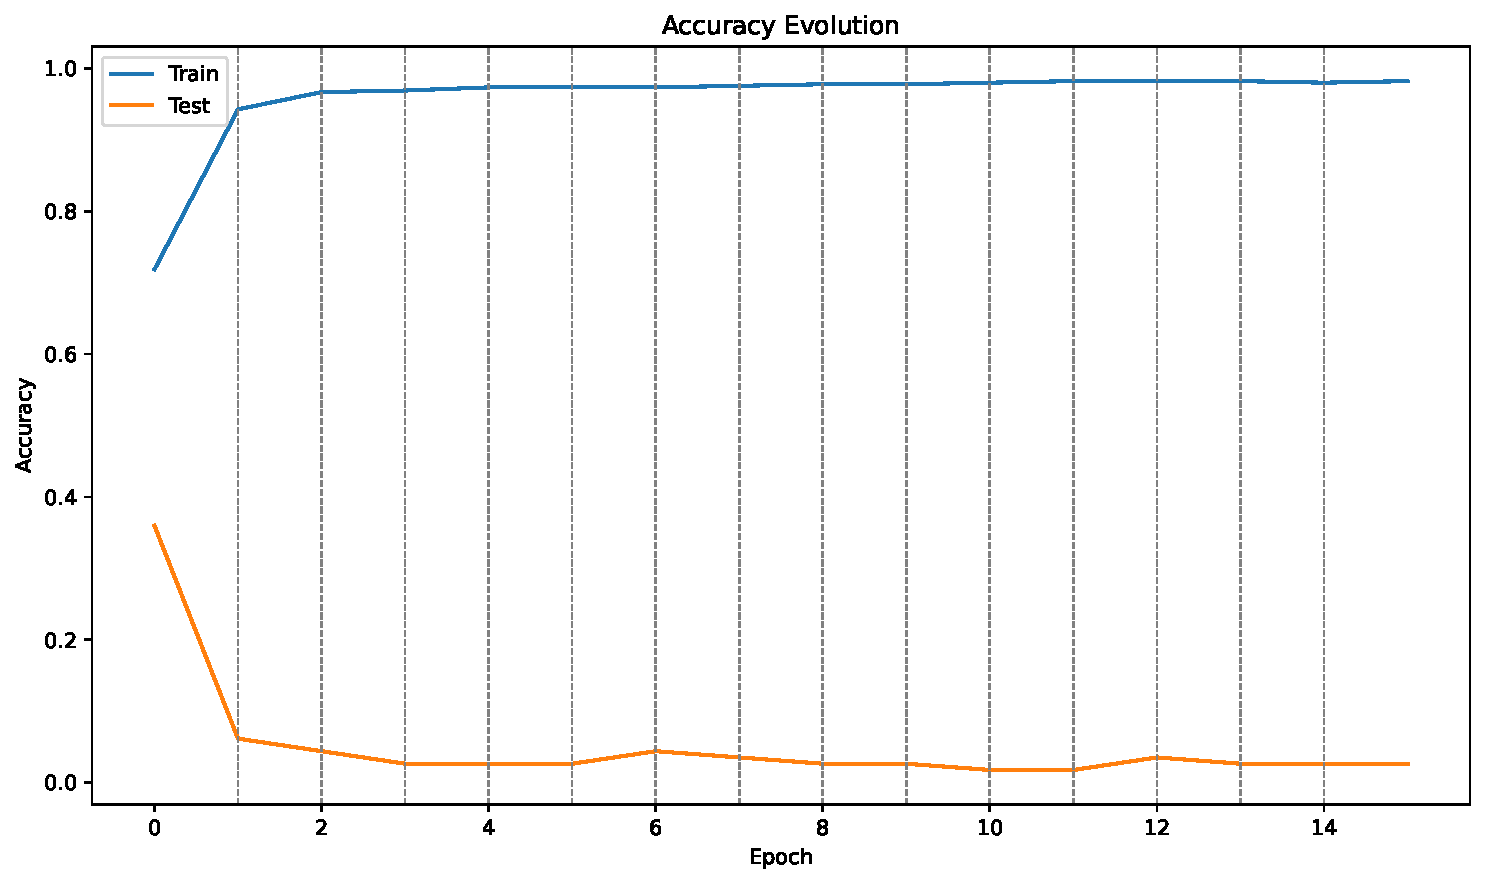
\includegraphics[width=\textwidth]{plots_v2/Cancer/eps=0.1/accuracy_evolution-t-d.pdf}
  \caption{Clean Features and Corrupted Labels}
\end{subfigure}
\begin{subfigure}[b]{0.32\textwidth}
  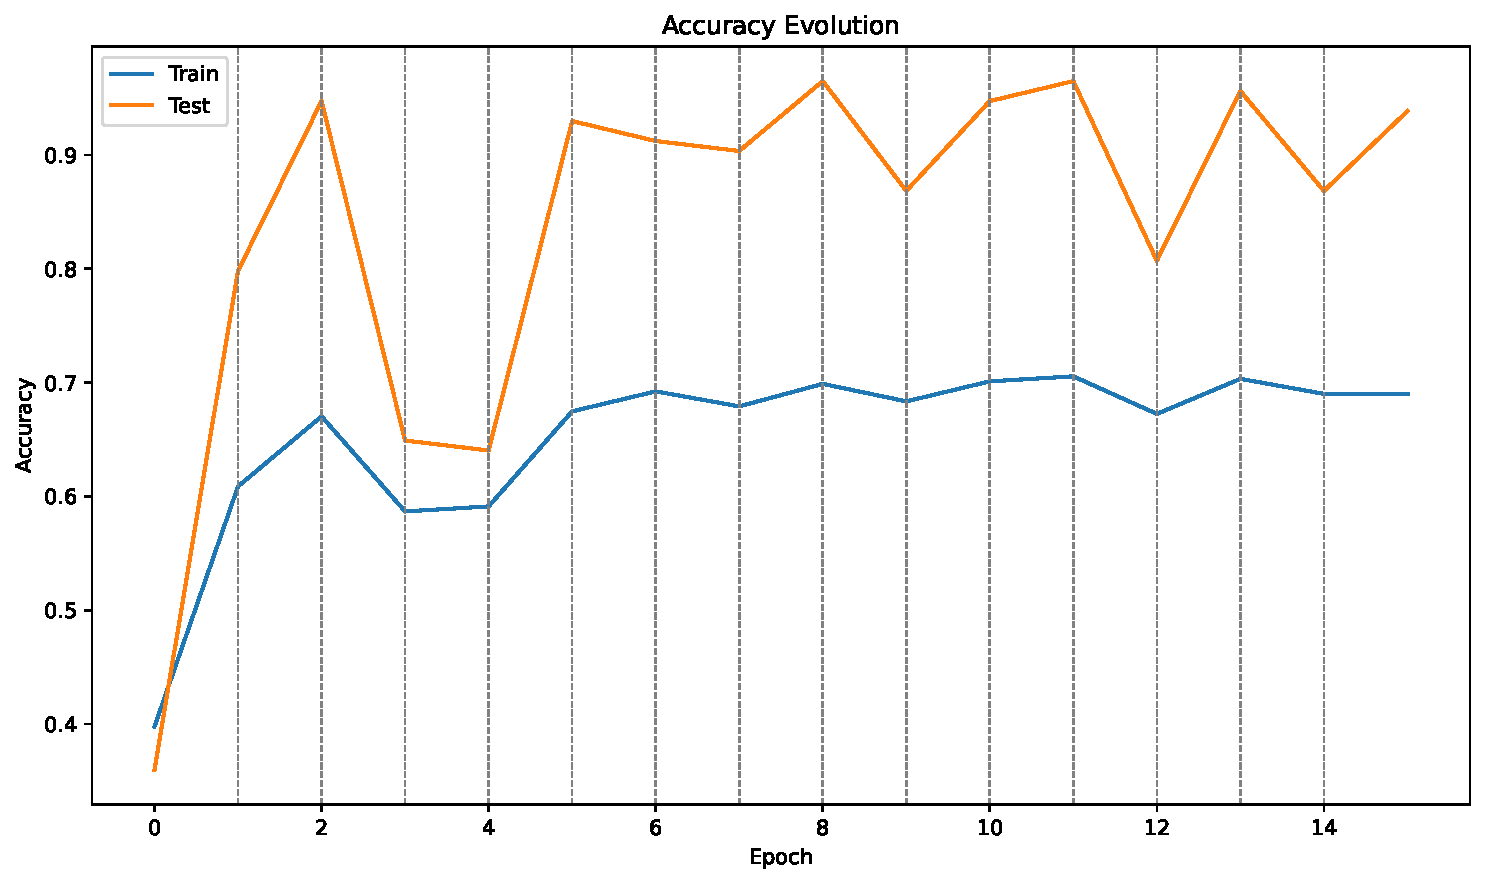
\includegraphics[width=\textwidth]{plots_v2/Cancer/eps=0.1/accuracy_evolution-t-v.pdf}
  \caption{Clean Features and Noisy Labels}
\end{subfigure}
\begin{subfigure}[b]{0.32\textwidth}
  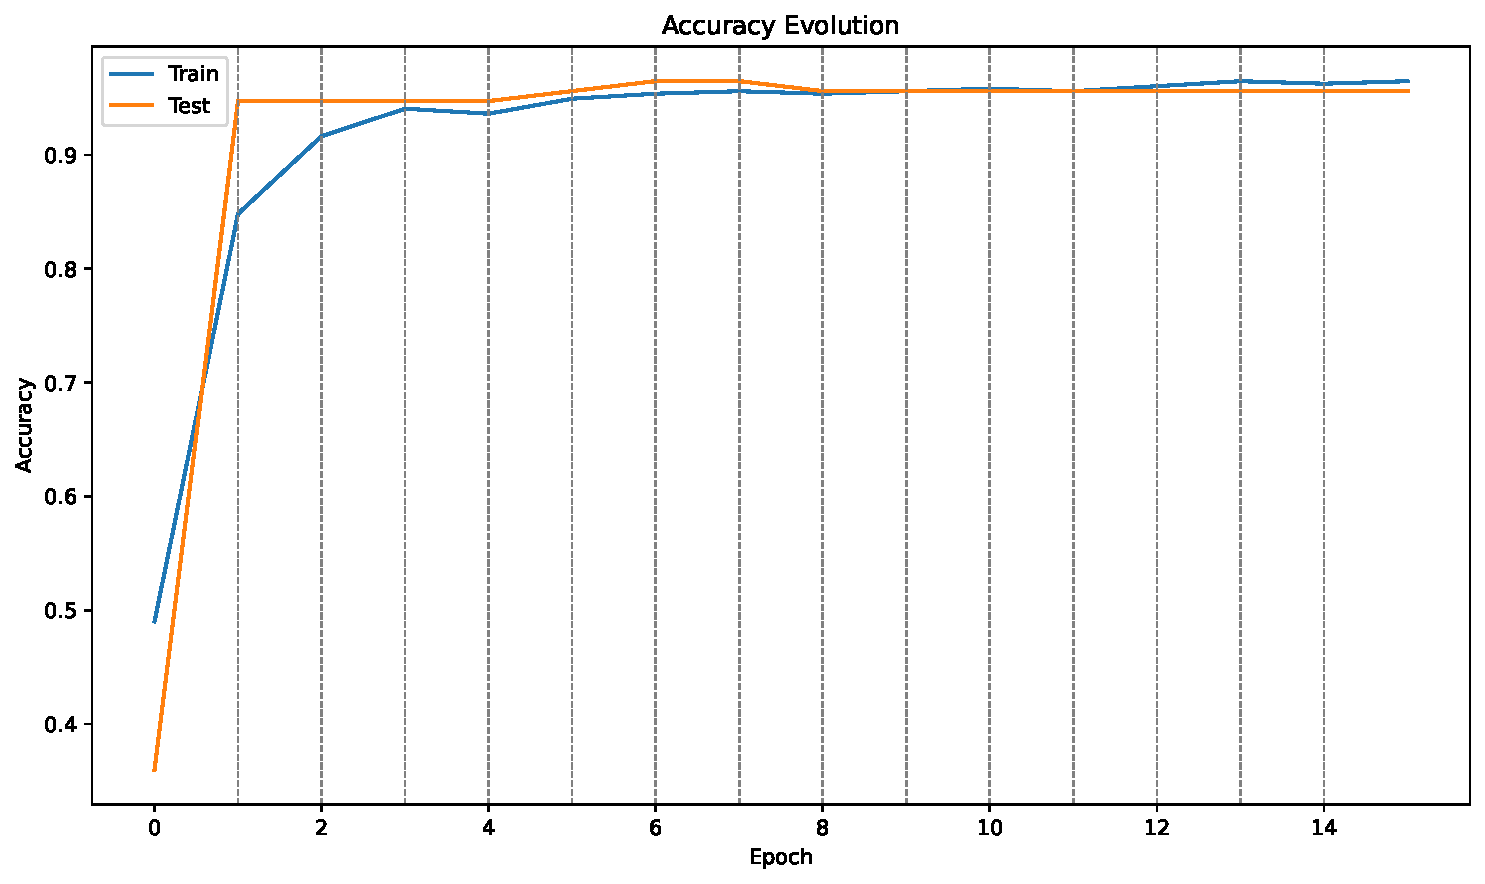
\includegraphics[width=\textwidth]{plots_v2/Cancer/eps=0.1/accuracy_evolution-v-t.pdf}
  \caption{Noisy Features and Clean Labels}
\end{subfigure}
\begin{subfigure}[b]{0.32\textwidth}
  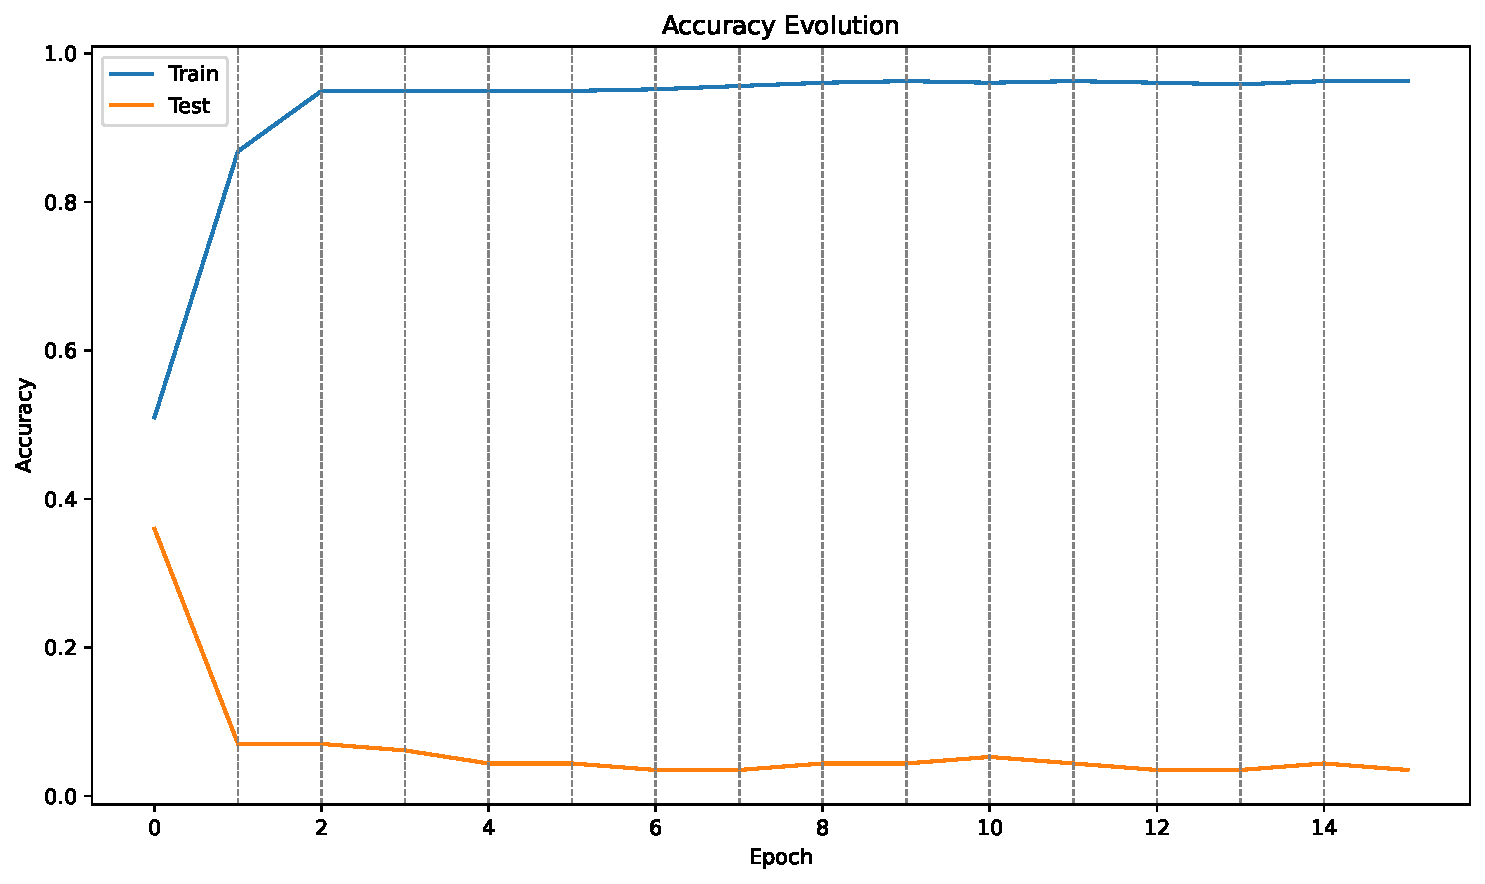
\includegraphics[width=\textwidth]{plots_v2/Cancer/eps=0.1/accuracy_evolution-v-d.pdf}
  \caption{Noisy Features and Corrupted Labels}
\end{subfigure}
\begin{subfigure}[b]{0.32\textwidth}
  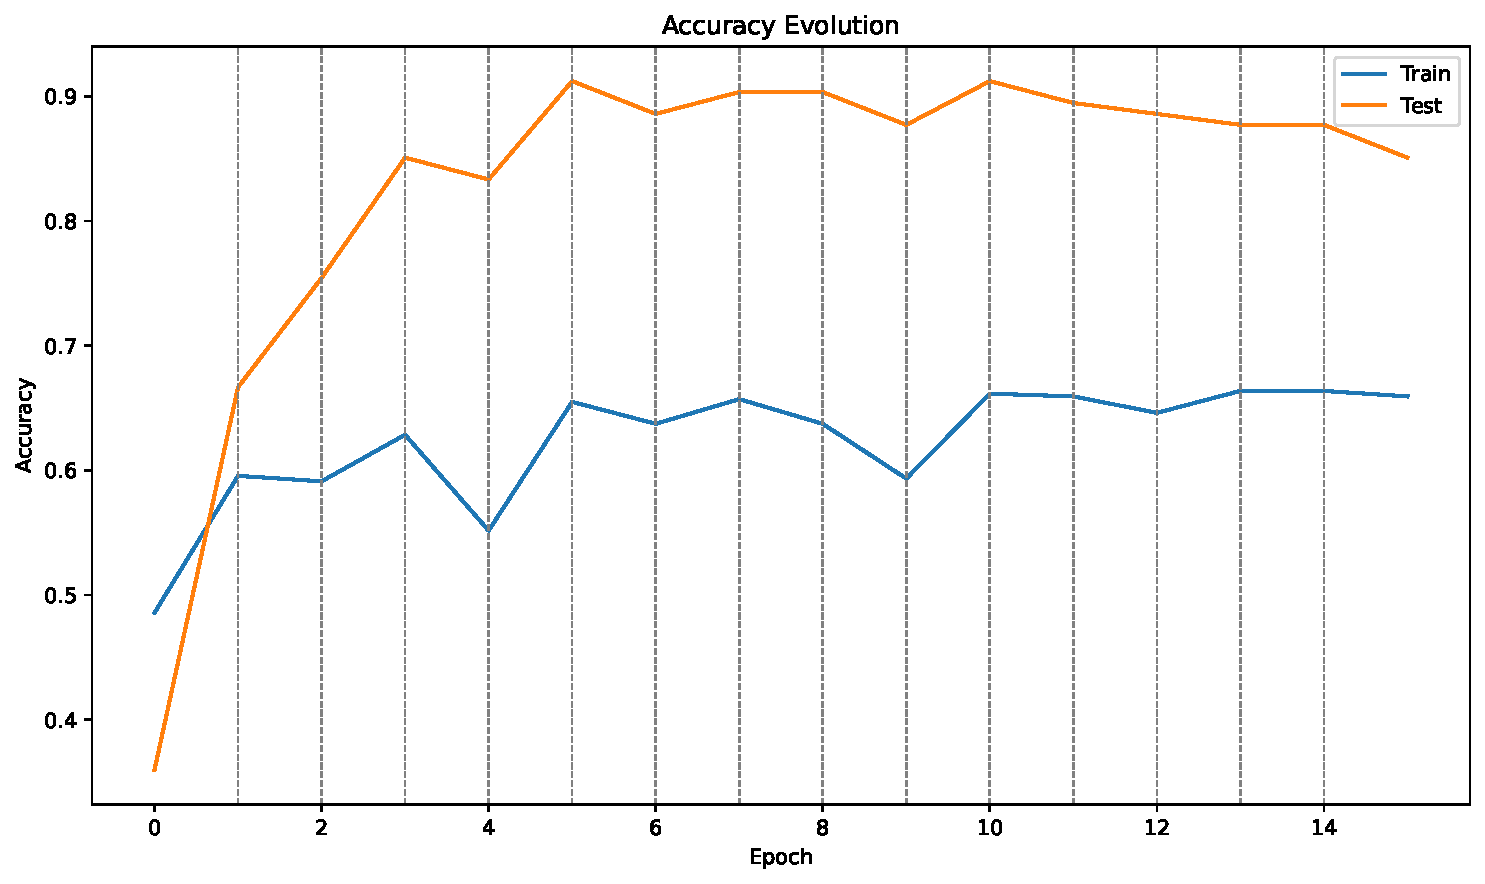
\includegraphics[width=\textwidth]{plots_v2/Cancer/eps=0.1/accuracy_evolution-v-v.pdf}
  \caption{Noisy Features and Noisy Labels}
\end{subfigure}
\begin{subfigure}[b]{0.32\textwidth}
  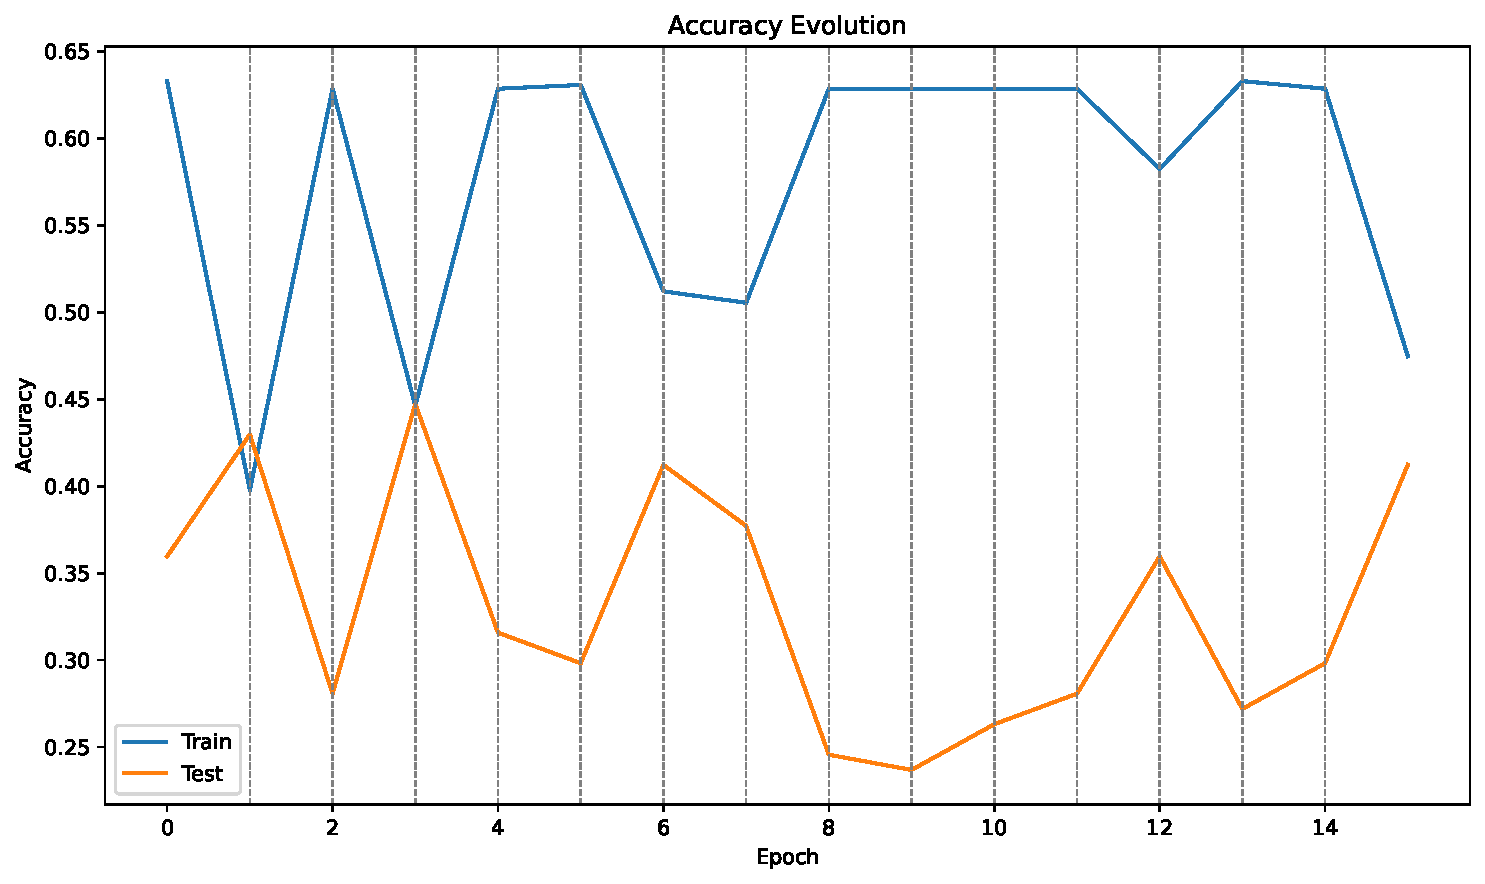
\includegraphics[width=\textwidth]{plots_v2/Cancer/eps=0.1/accuracy_evolution-d-t.pdf}
  \caption{Corrupted Features and Clean Labels}
\end{subfigure}
\begin{subfigure}[b]{0.32\textwidth}
  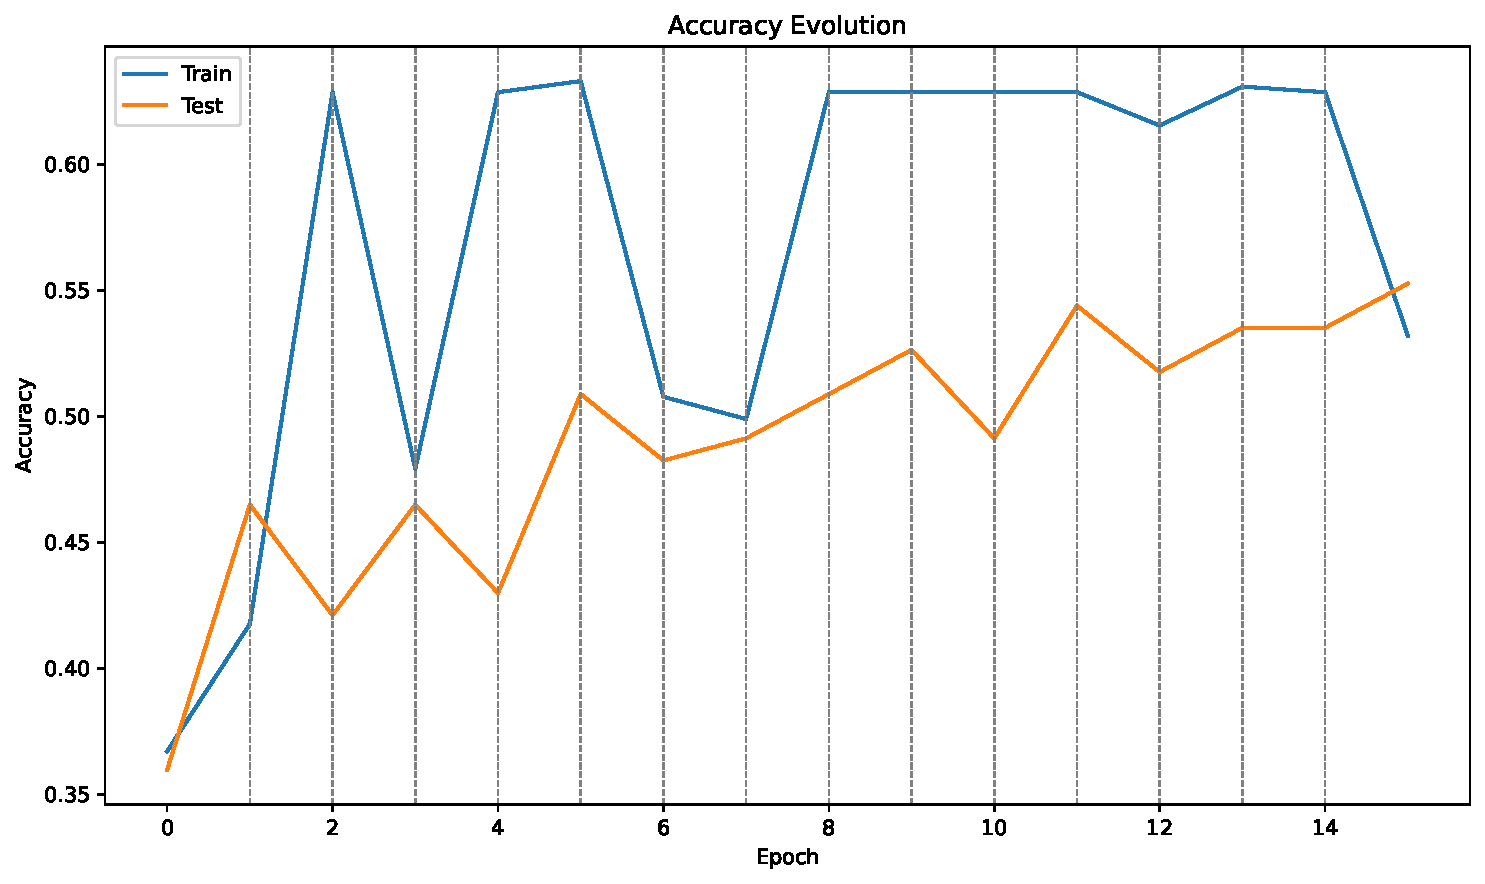
\includegraphics[width=\textwidth]{plots_v2/Cancer/eps=0.1/accuracy_evolution-d-d.pdf}
  \caption{Corrupted Features and Corrupted Labels}
\end{subfigure}
\begin{subfigure}[b]{0.32\textwidth}
  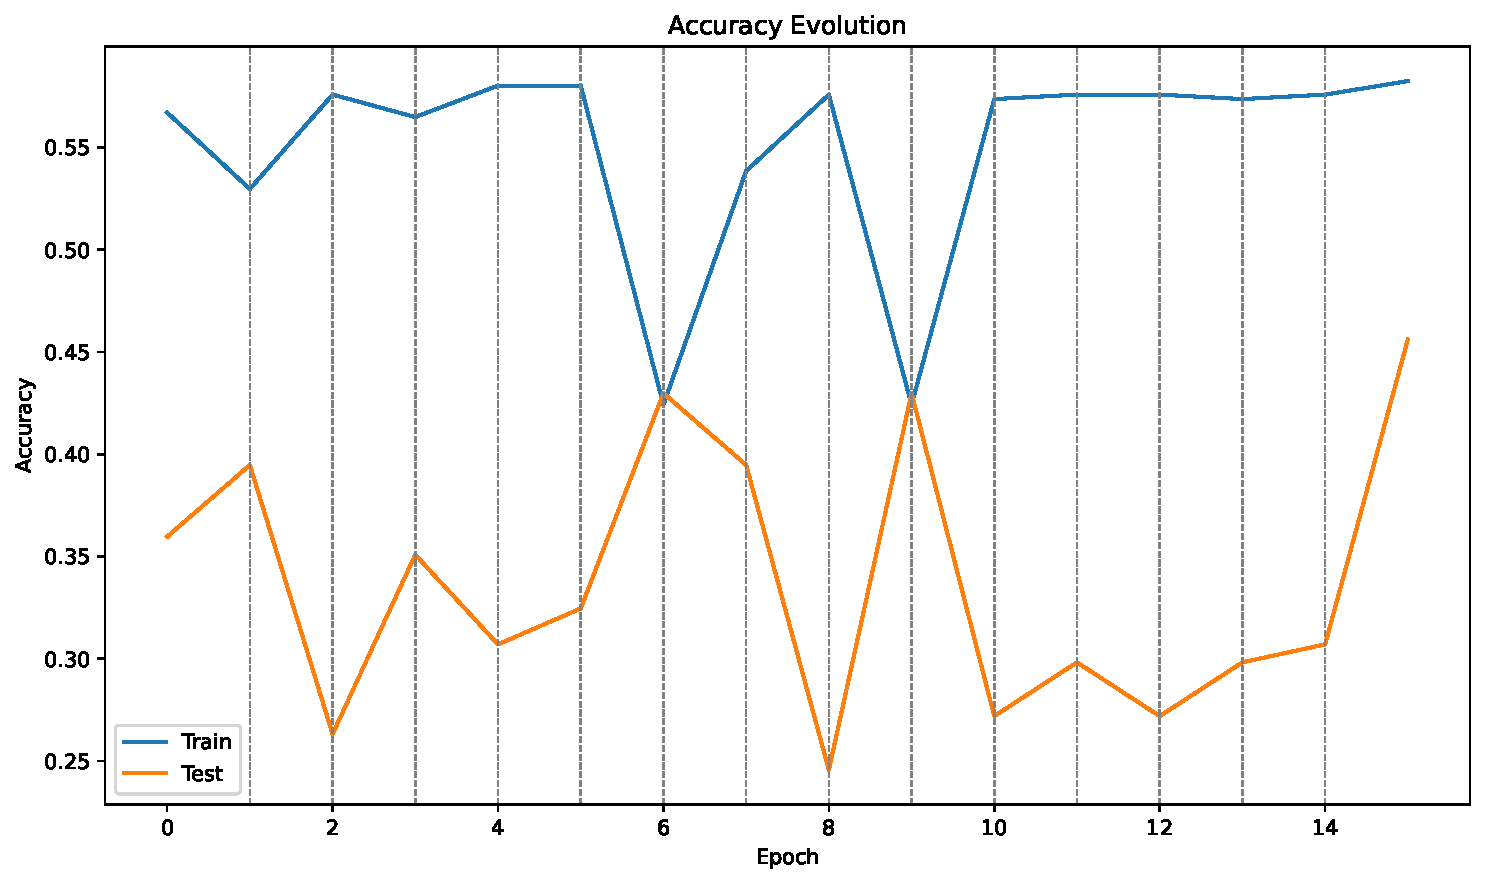
\includegraphics[width=\textwidth]{plots_v2/Cancer/eps=0.1/accuracy_evolution-d-v.pdf}
  \caption{Corrupted Features and Noisy Labels}
\end{subfigure}
\caption{Accuracy evolution of the Cancer model under different combinations of clean, corrupted, and noisy features and labels.}
\label{fig:Acccancer}
\end{figure}
% \begin{figure}[H]
%     \centering
%     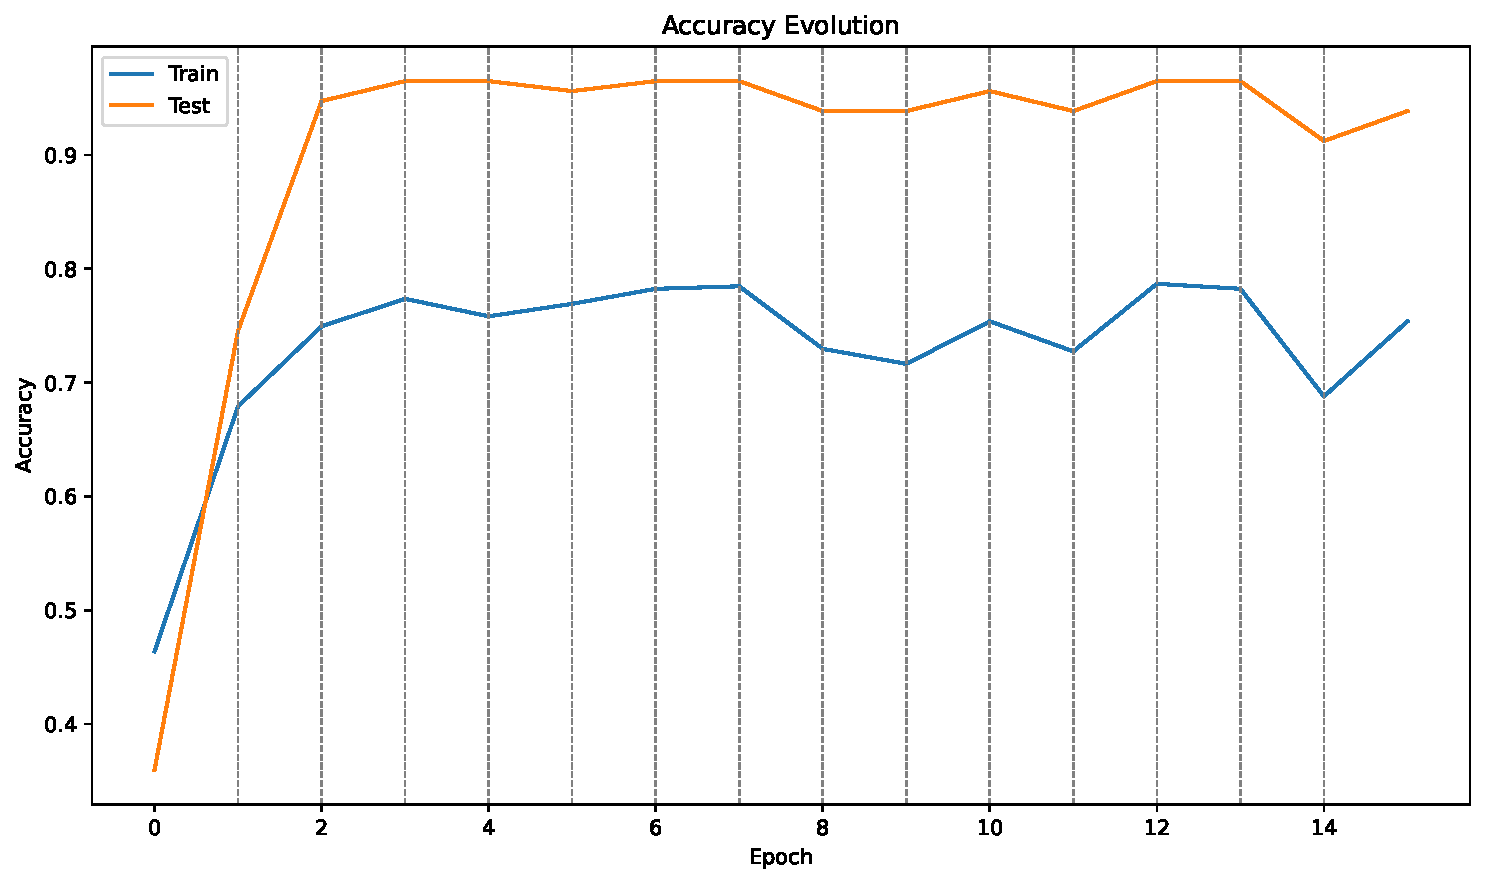
\includegraphics[width=0.8\linewidth]{good_plots/accuracy/Cancer/0.15-0.25/Cancer-noise-noise.pdf}
%     \caption{Accuracy evolution of the Cancer model when reducing the noise for noised features and labels.}
%     \label{fig:AcccancerInt}
% \end{figure}

\subsection{MNIST with Vacuous Trust Assessment (\cref{exp:2})}\label{sec:resmnist}
\begin{figure}[H]
  \centering
  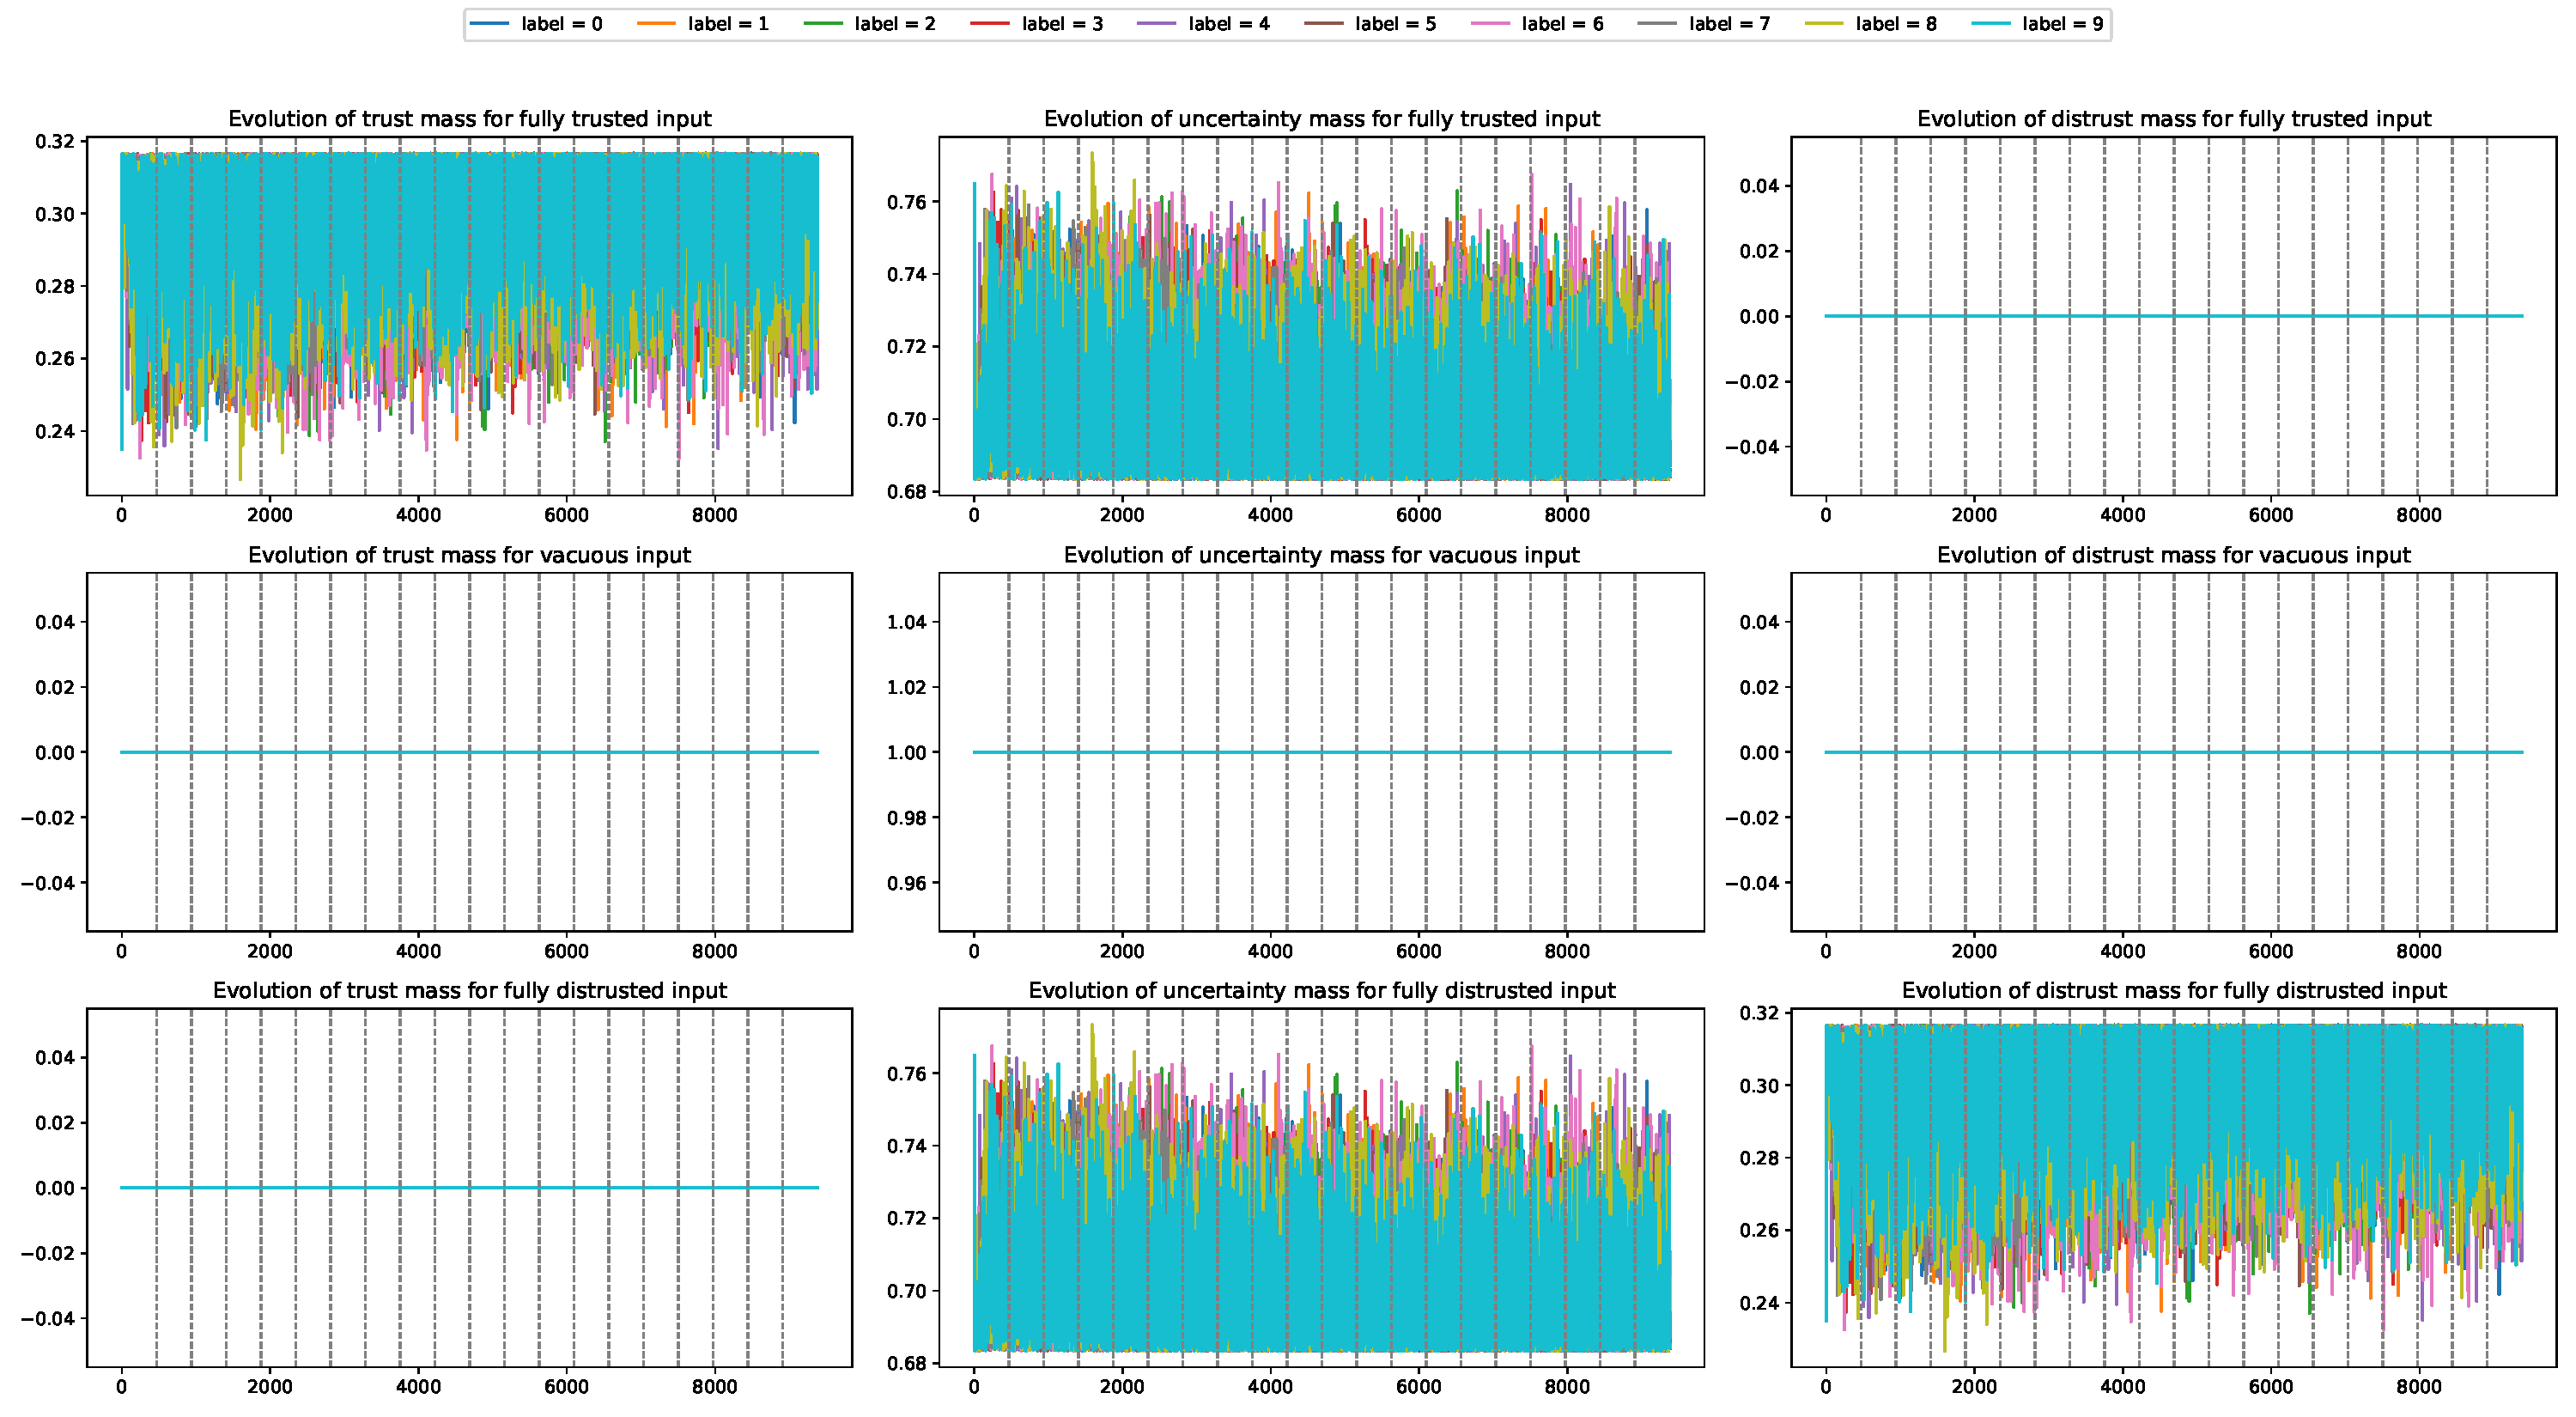
\includegraphics[width=\textwidth]{plots_v2/MNIST/architecture/plot_ptas-16-v-v.pdf}
  \caption{16 Hidden neurons}
\end{figure}
\begin{figure}[H]
  \centering
  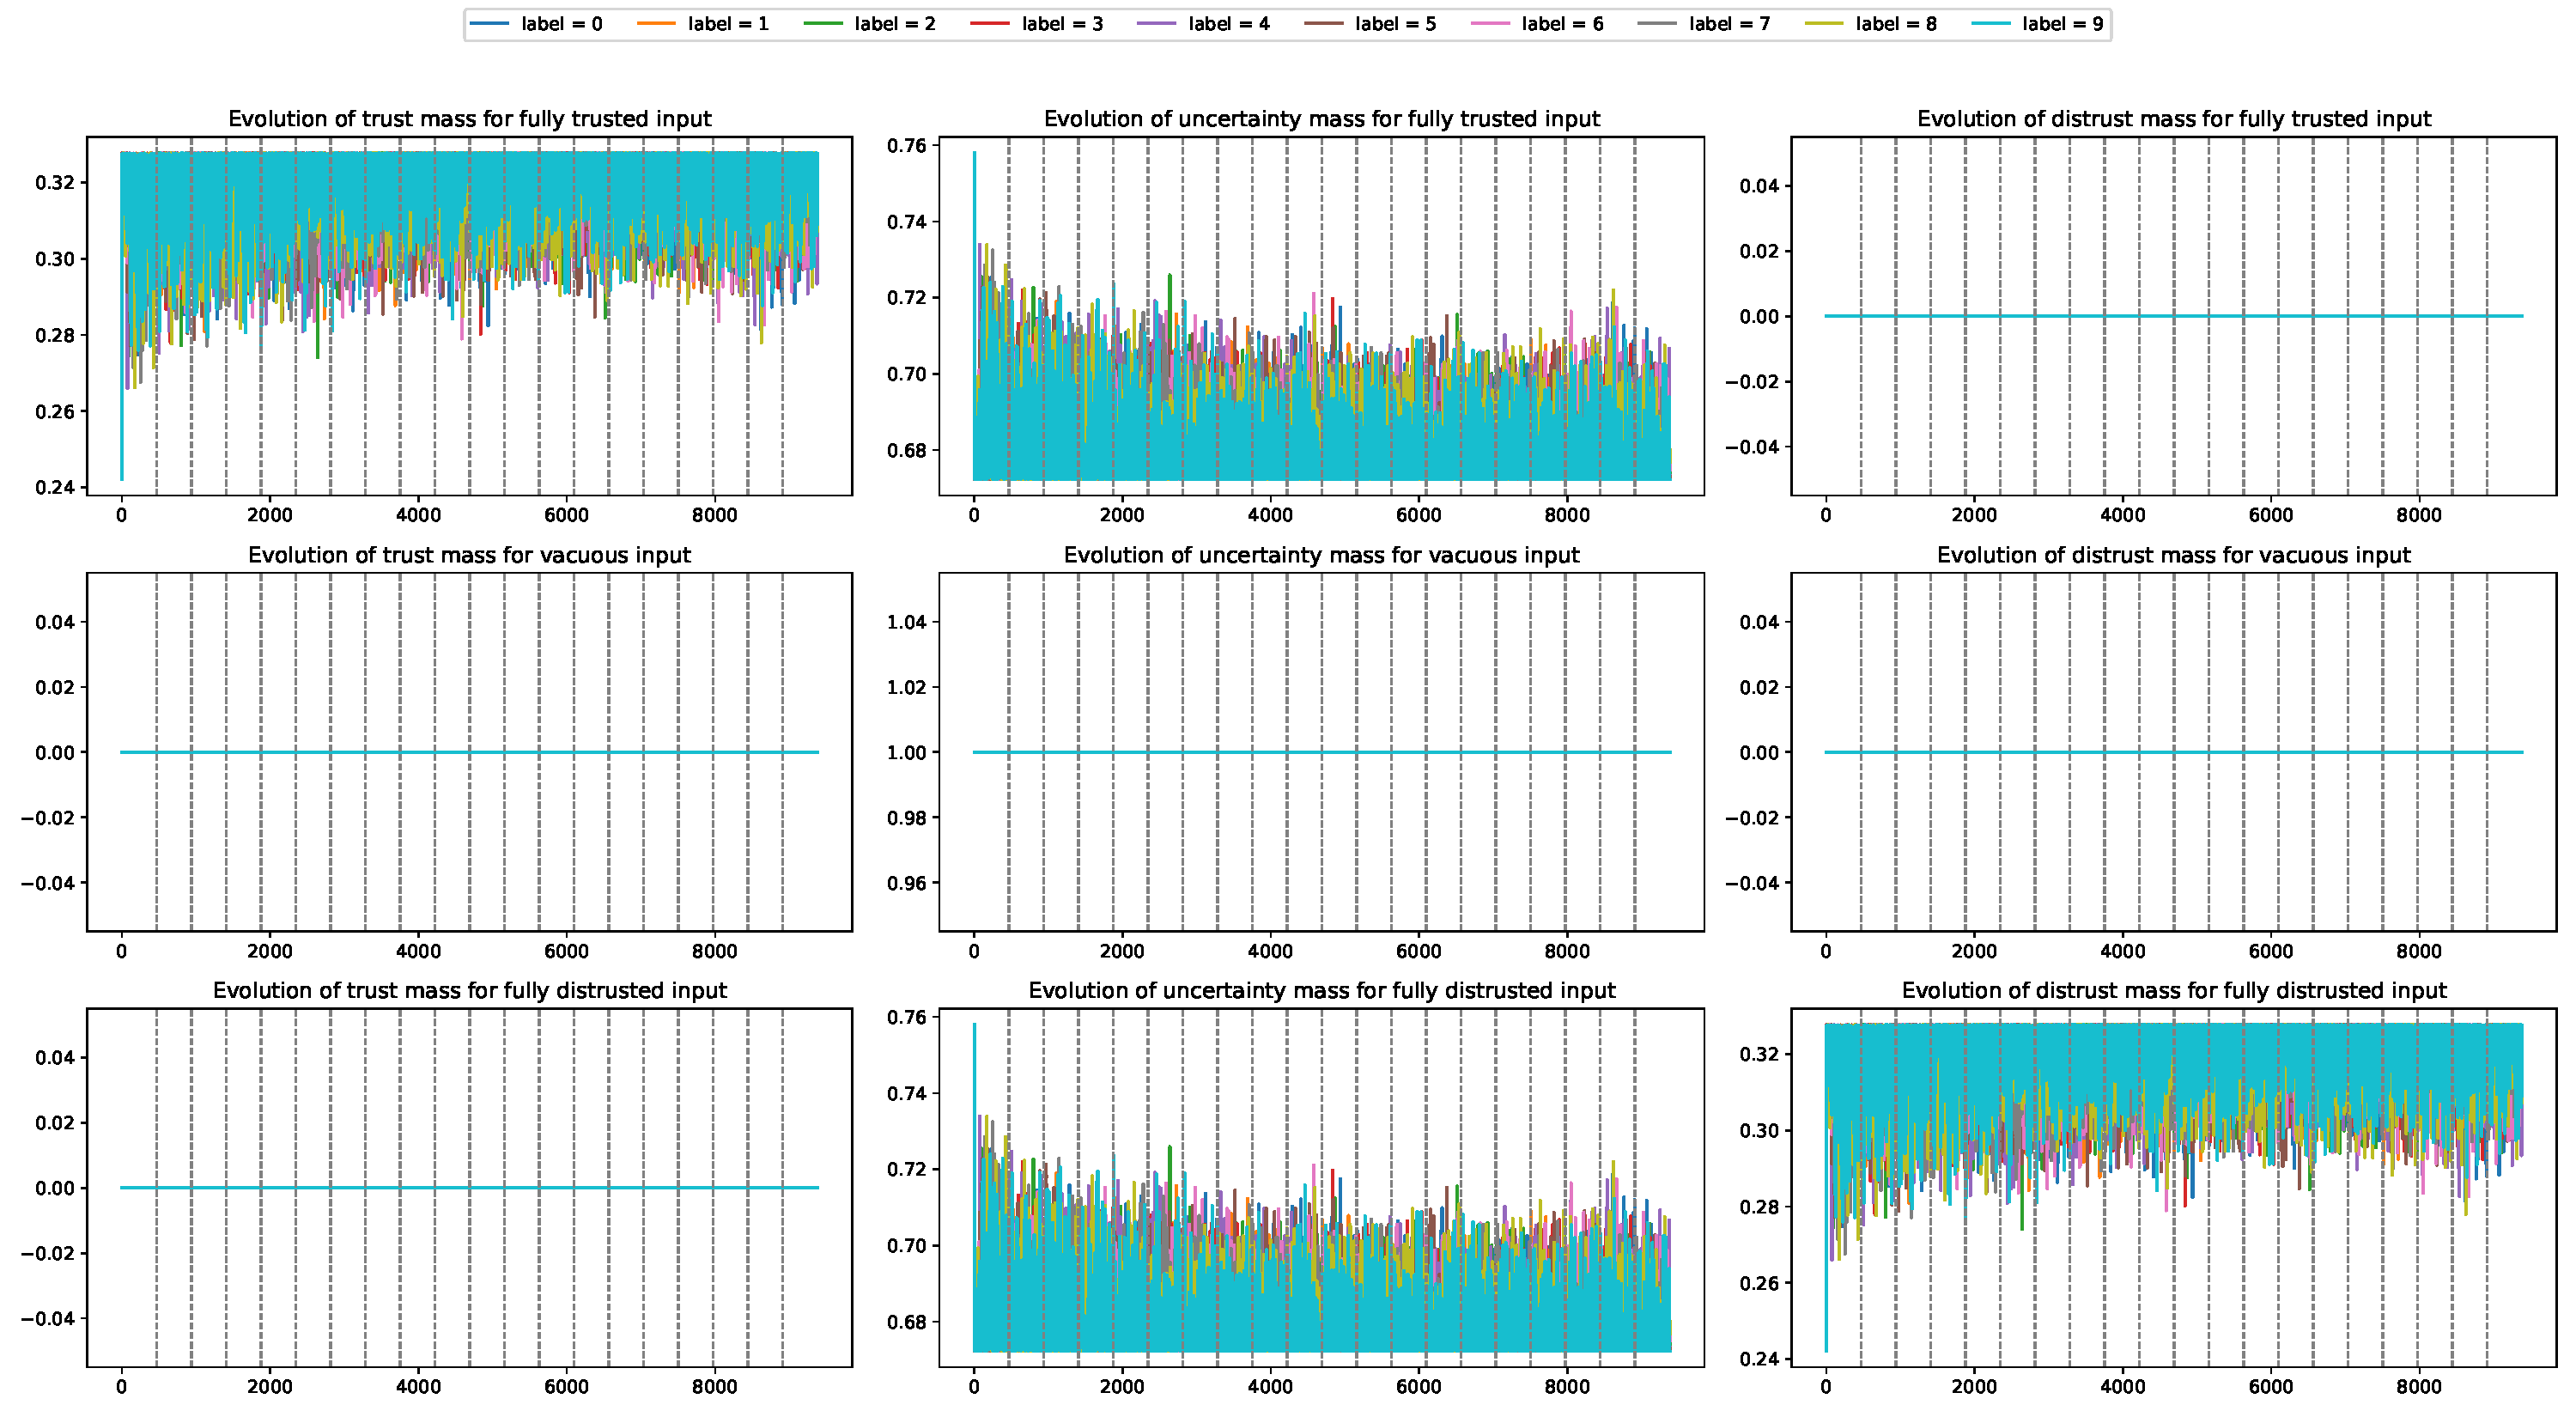
\includegraphics[width=\textwidth]{plots_v2/MNIST/architecture/plot_ptas-32-v-v.pdf}
  \caption{32 Hidden neurons}
\end{figure}
\begin{figure}[H]
  \centering
  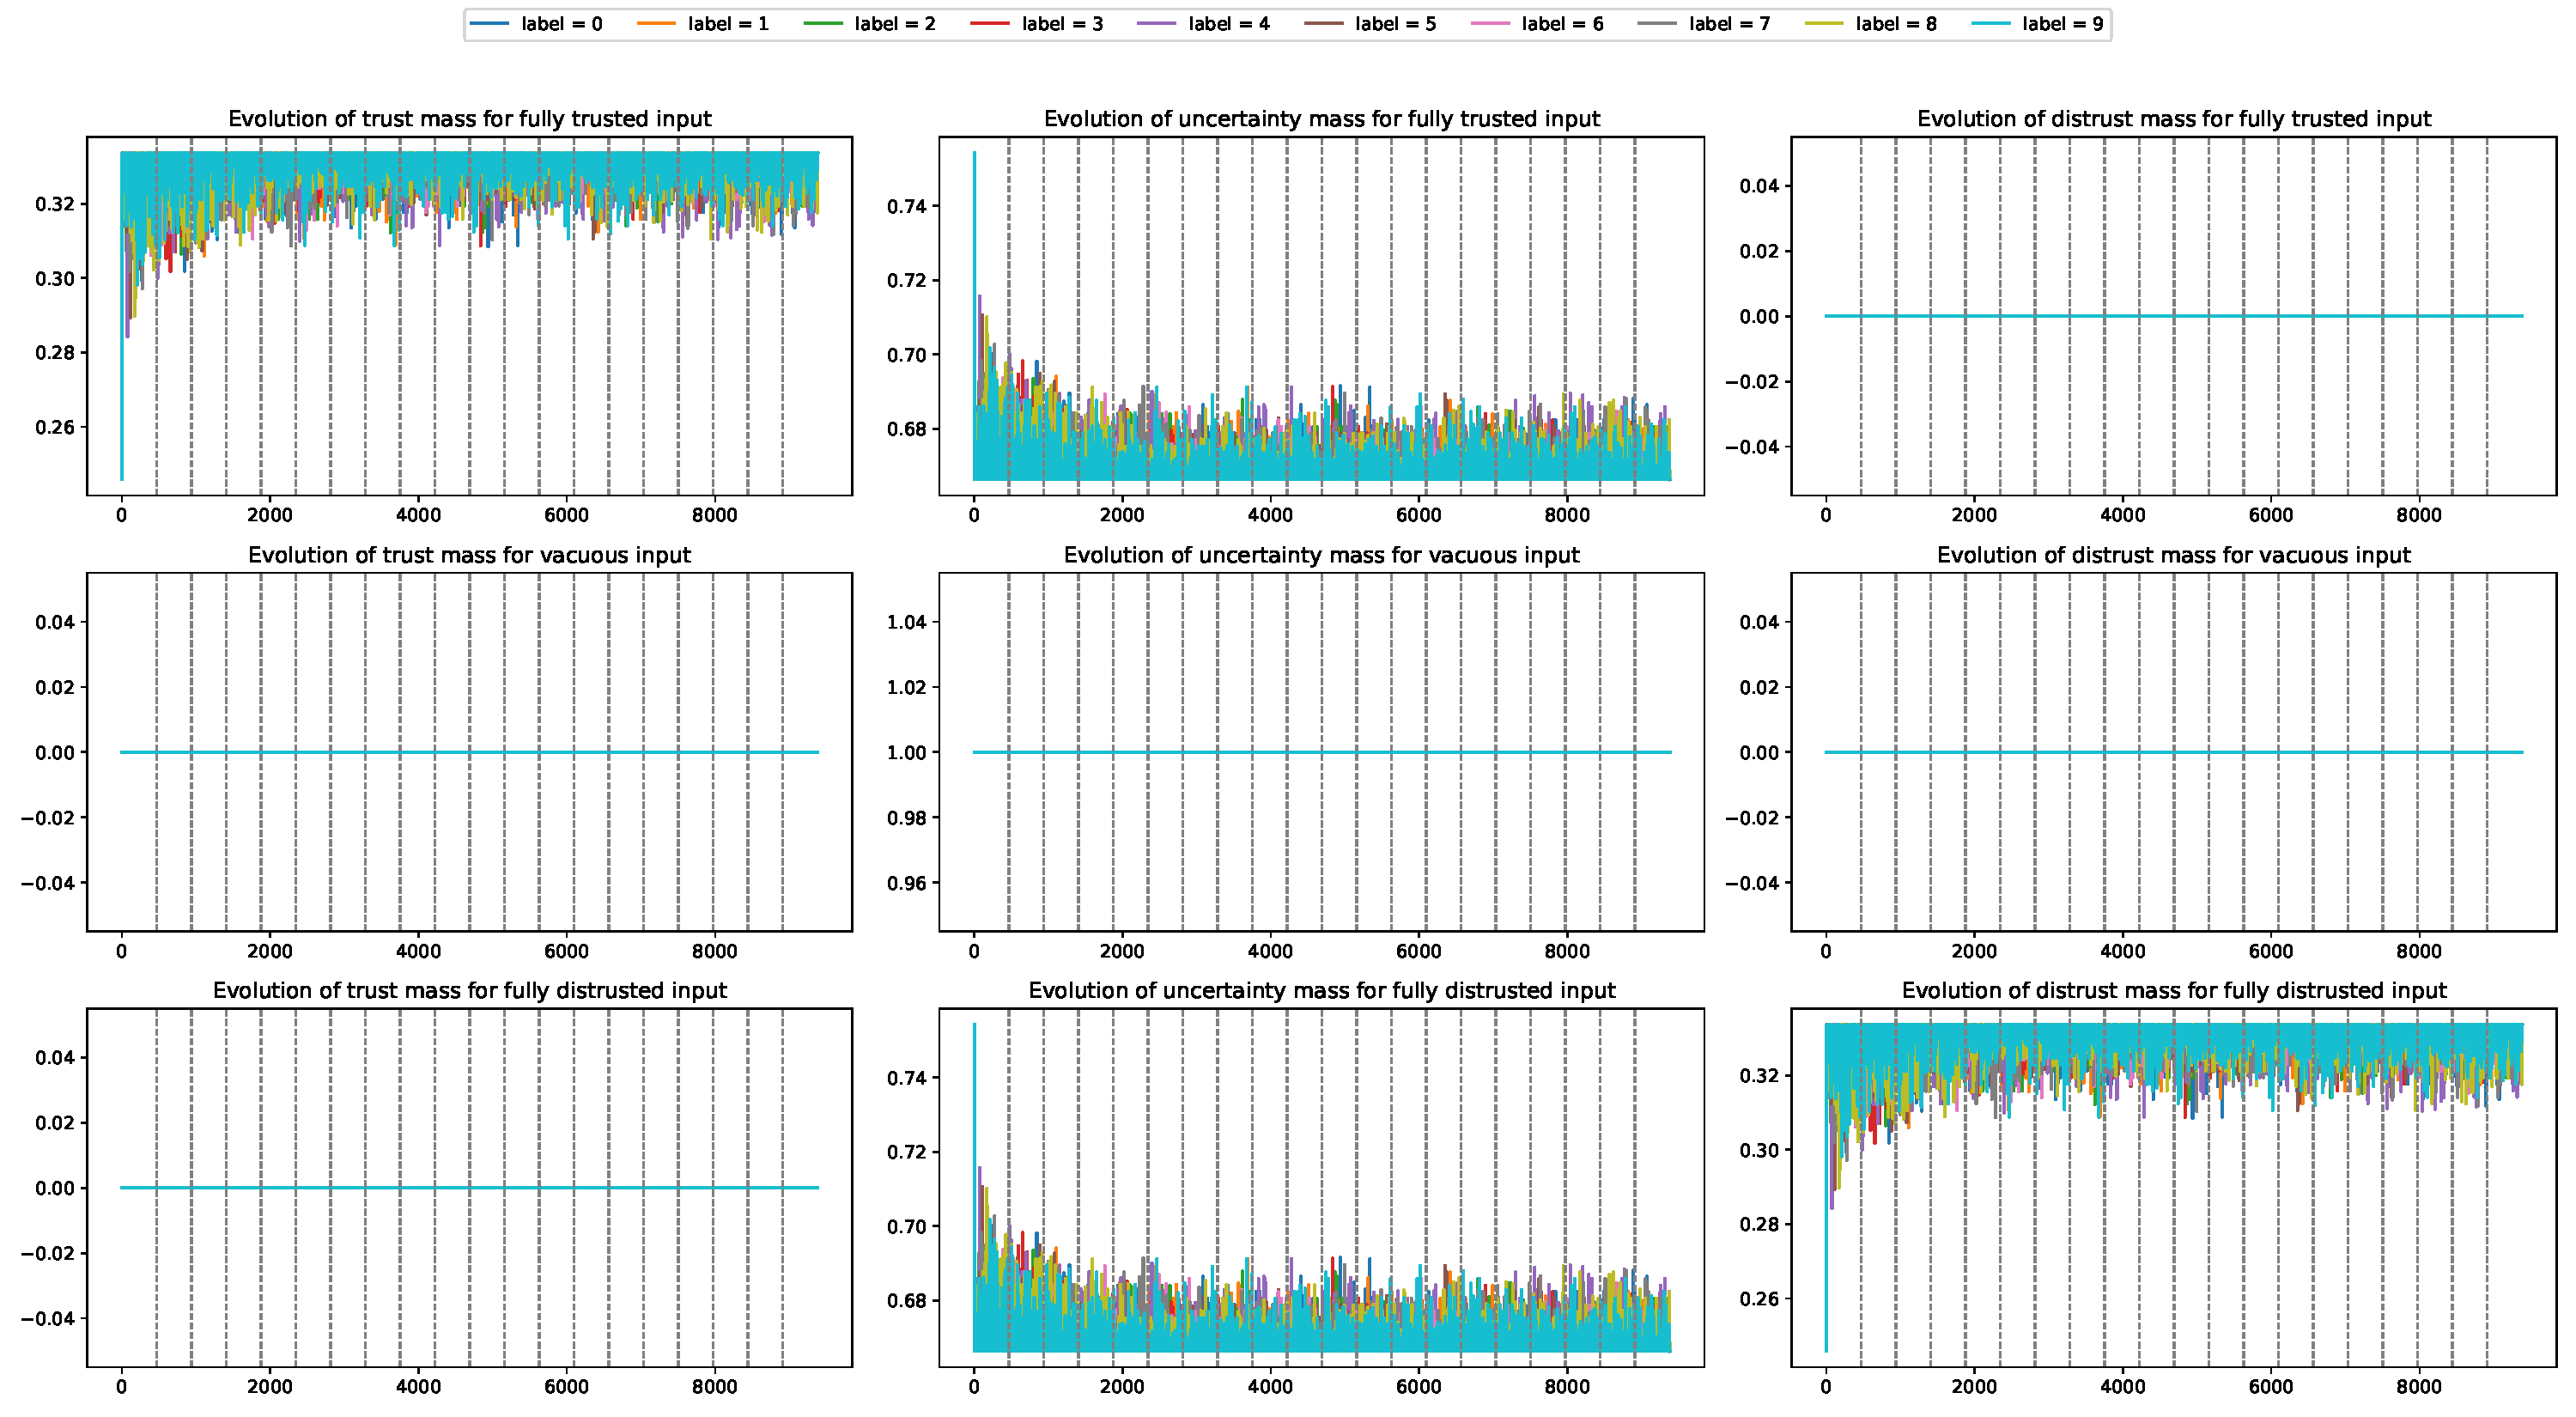
\includegraphics[width=\textwidth]{plots_v2/MNIST/architecture/plot_ptas-64-v-v.pdf}
  \caption{64 Hidden neurons}
\end{figure}
\begin{figure}[H]
  \centering
  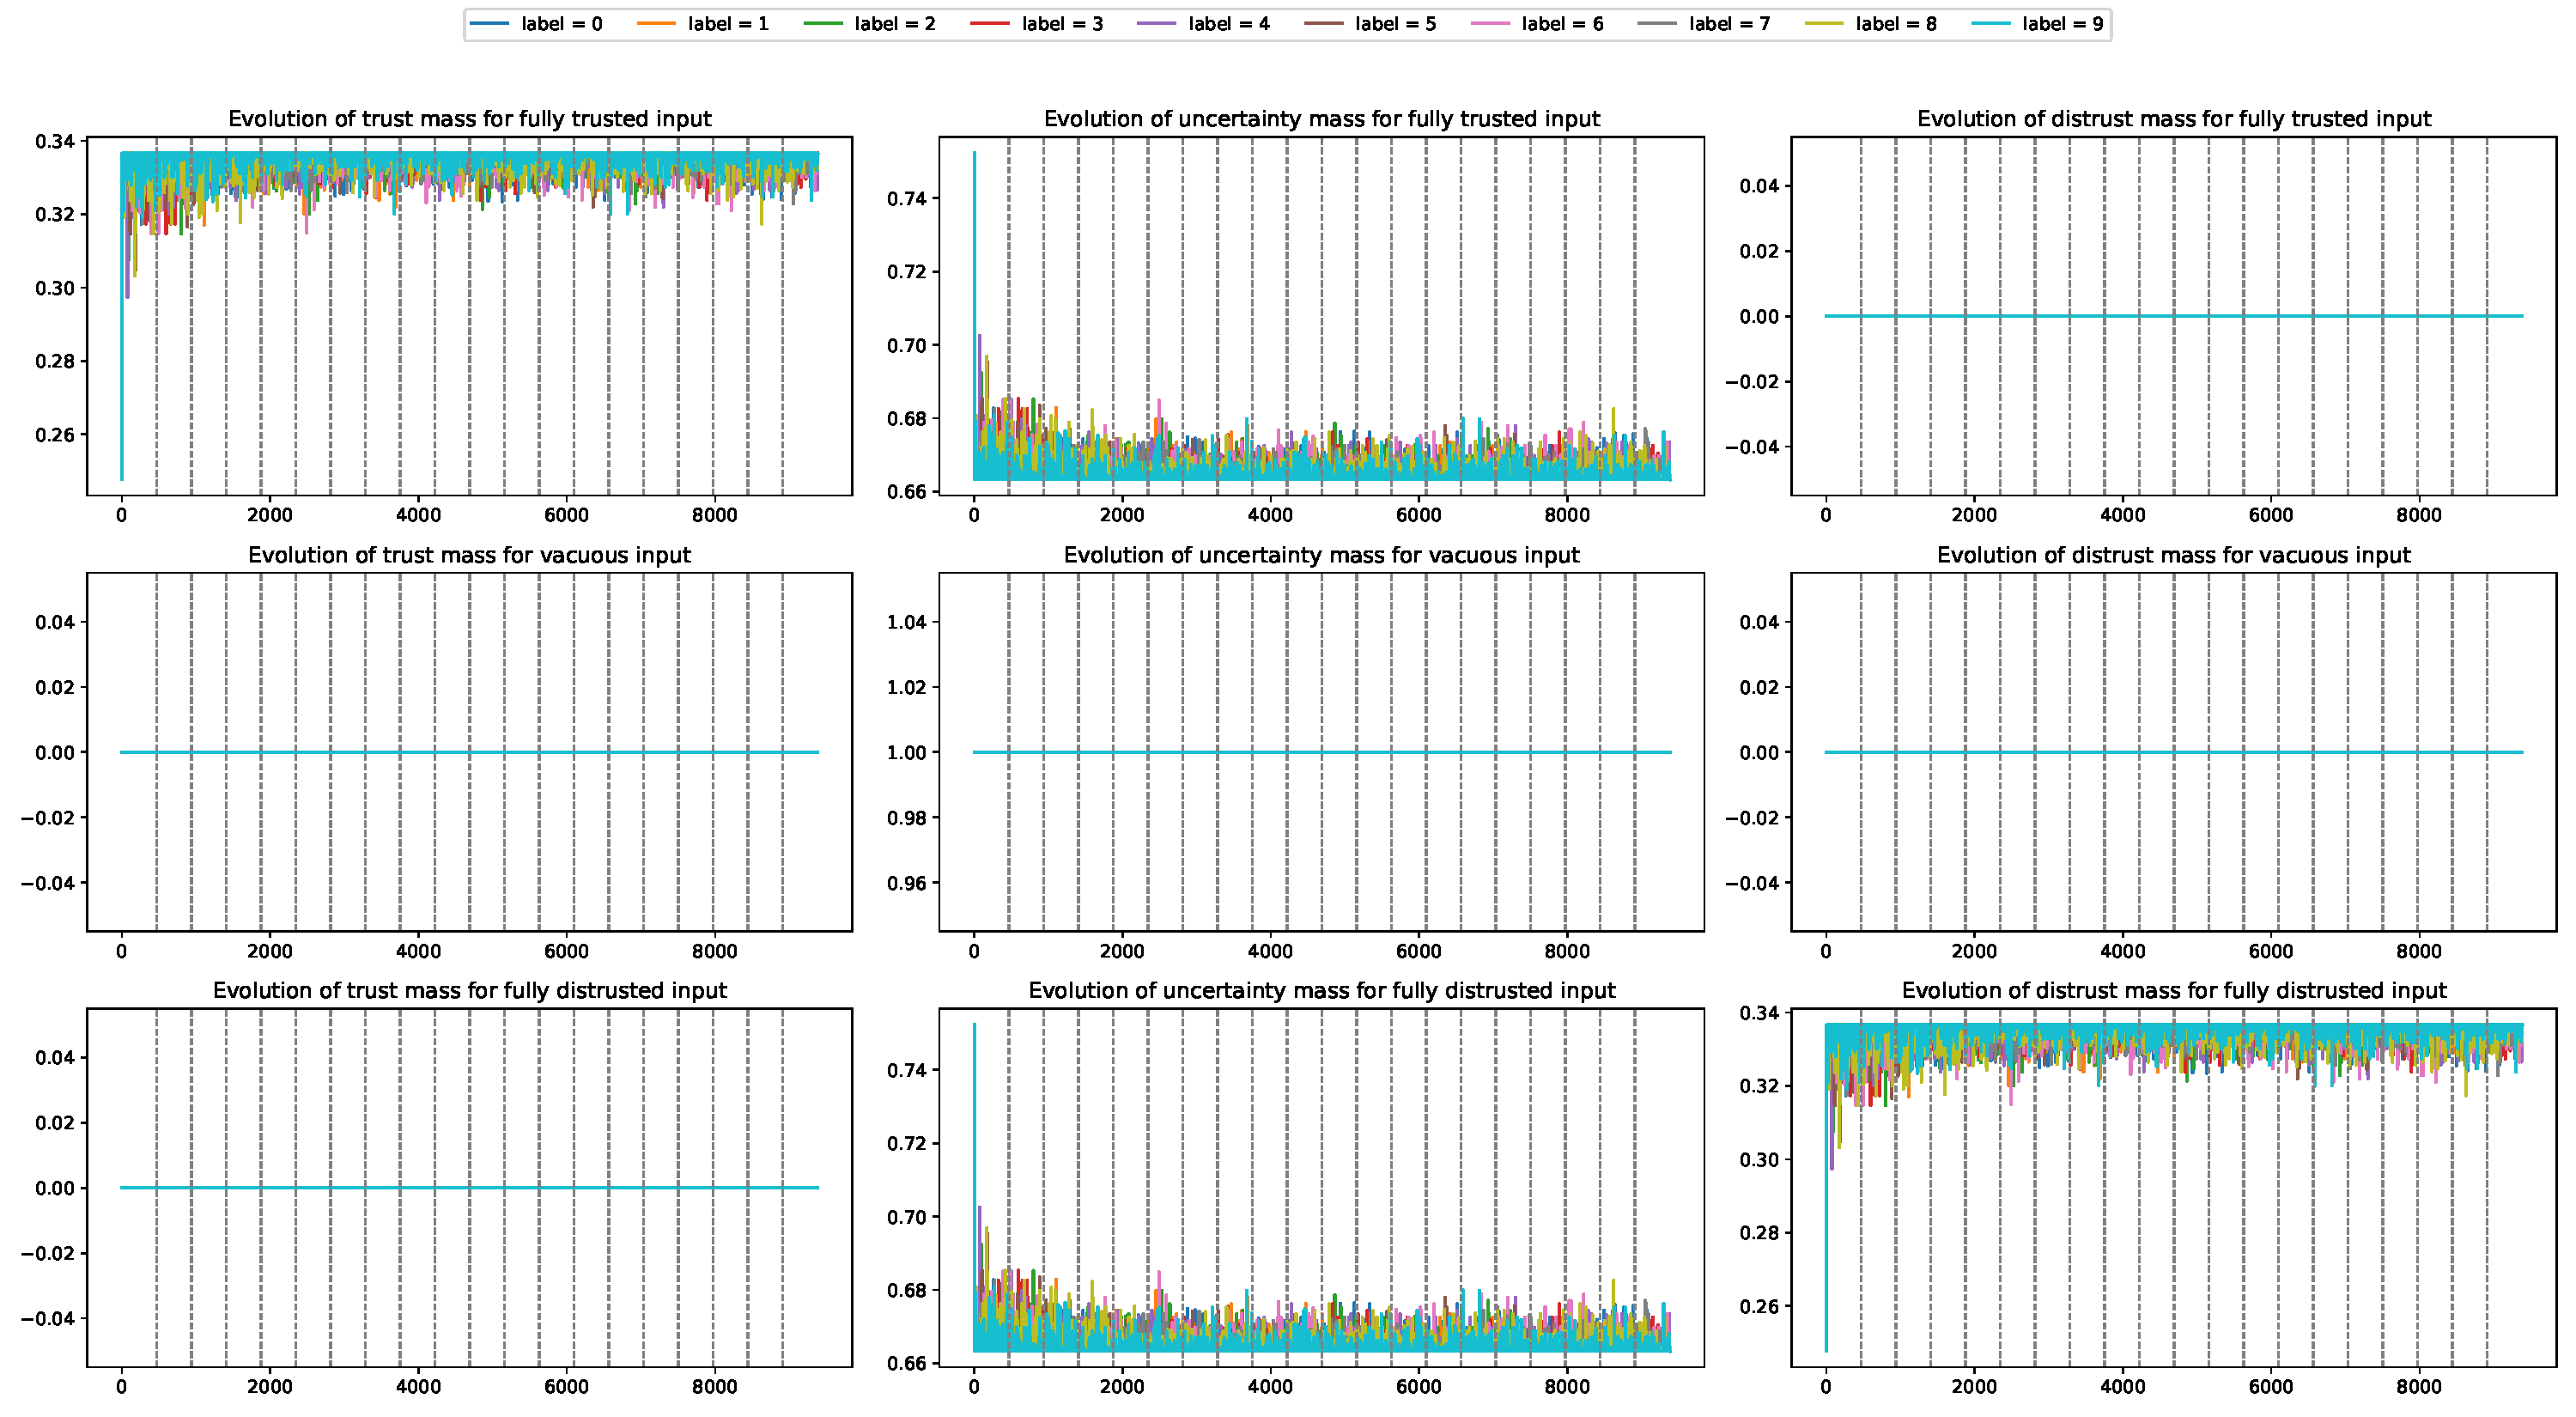
\includegraphics[width=\textwidth]{plots_v2/MNIST/architecture/plot_ptas-128-v-v.pdf}
  \caption{128 Hidden neurons}
\end{figure}
\begin{figure}[H]
  \centering
  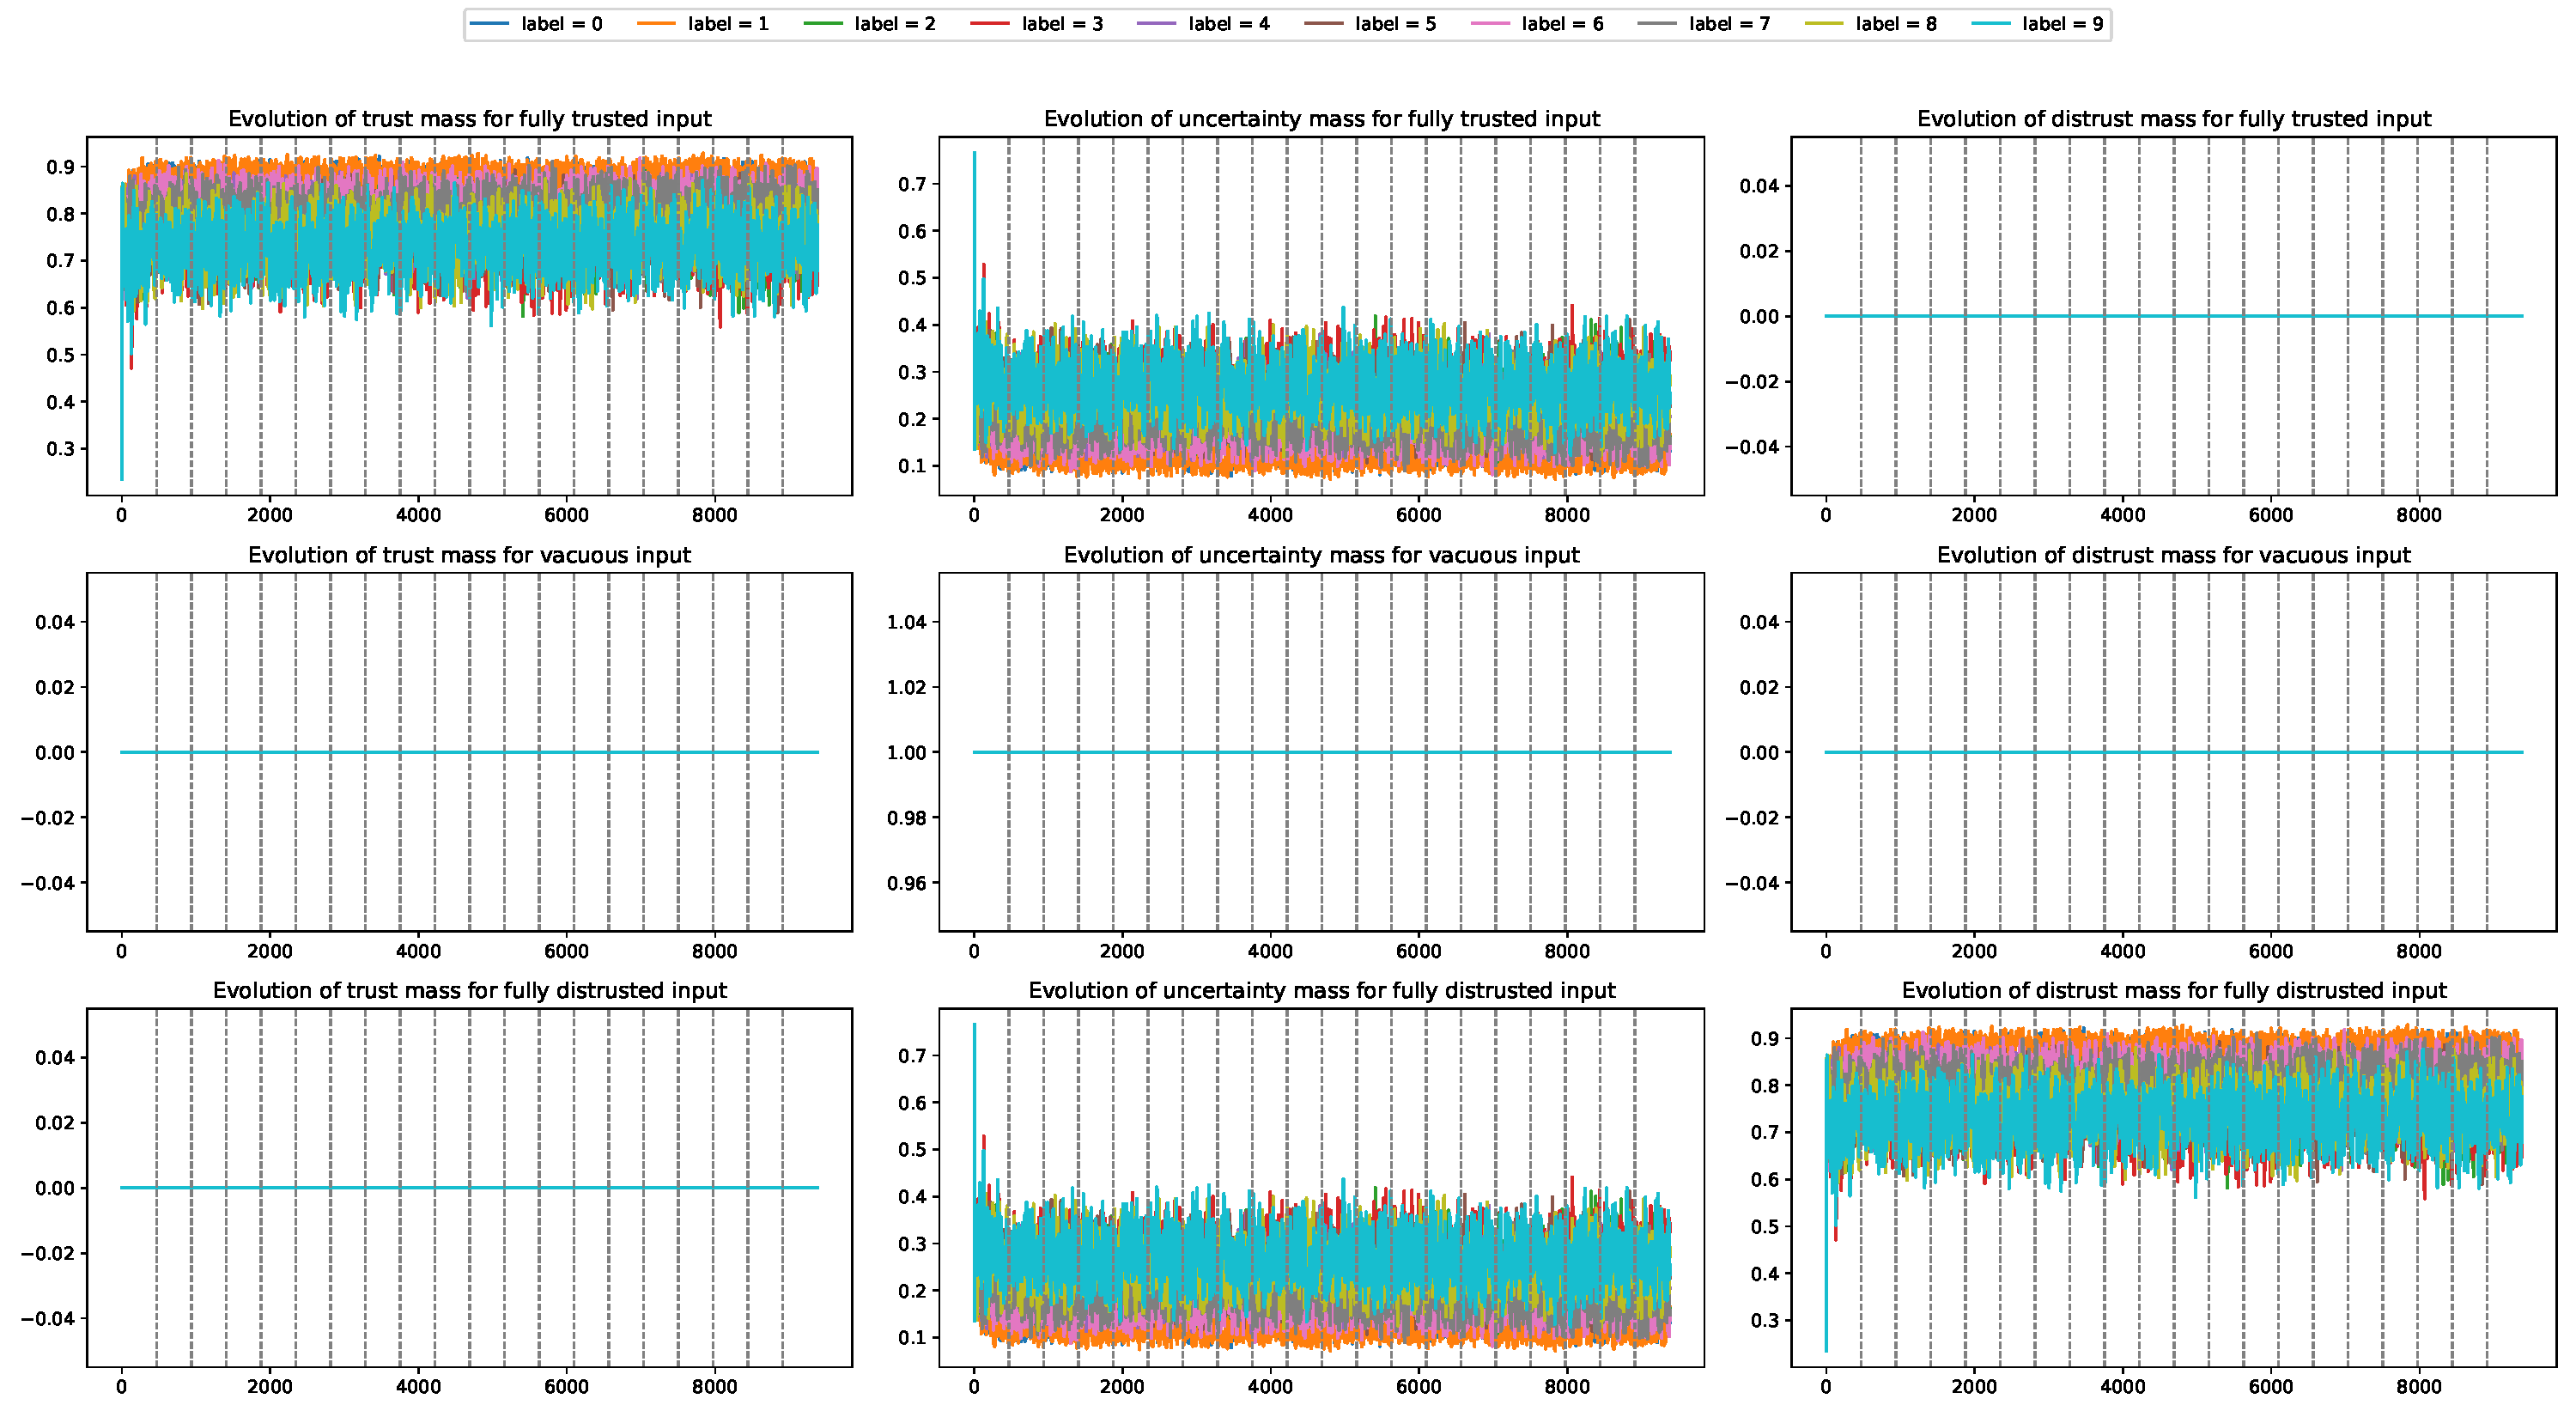
\includegraphics[width=\textwidth]{plots_v2/MNIST/architecture/plot_ptas-16-t-t.pdf}
  \caption{16 Hidden neurons with Fully Trusted Assessment}
\end{figure}

\subsection{MNIST poisoned 128 hidden neurons (\cref{exp:3})}\label{sec:resmnistpois}
\begin{figure}[H]
  \centering
  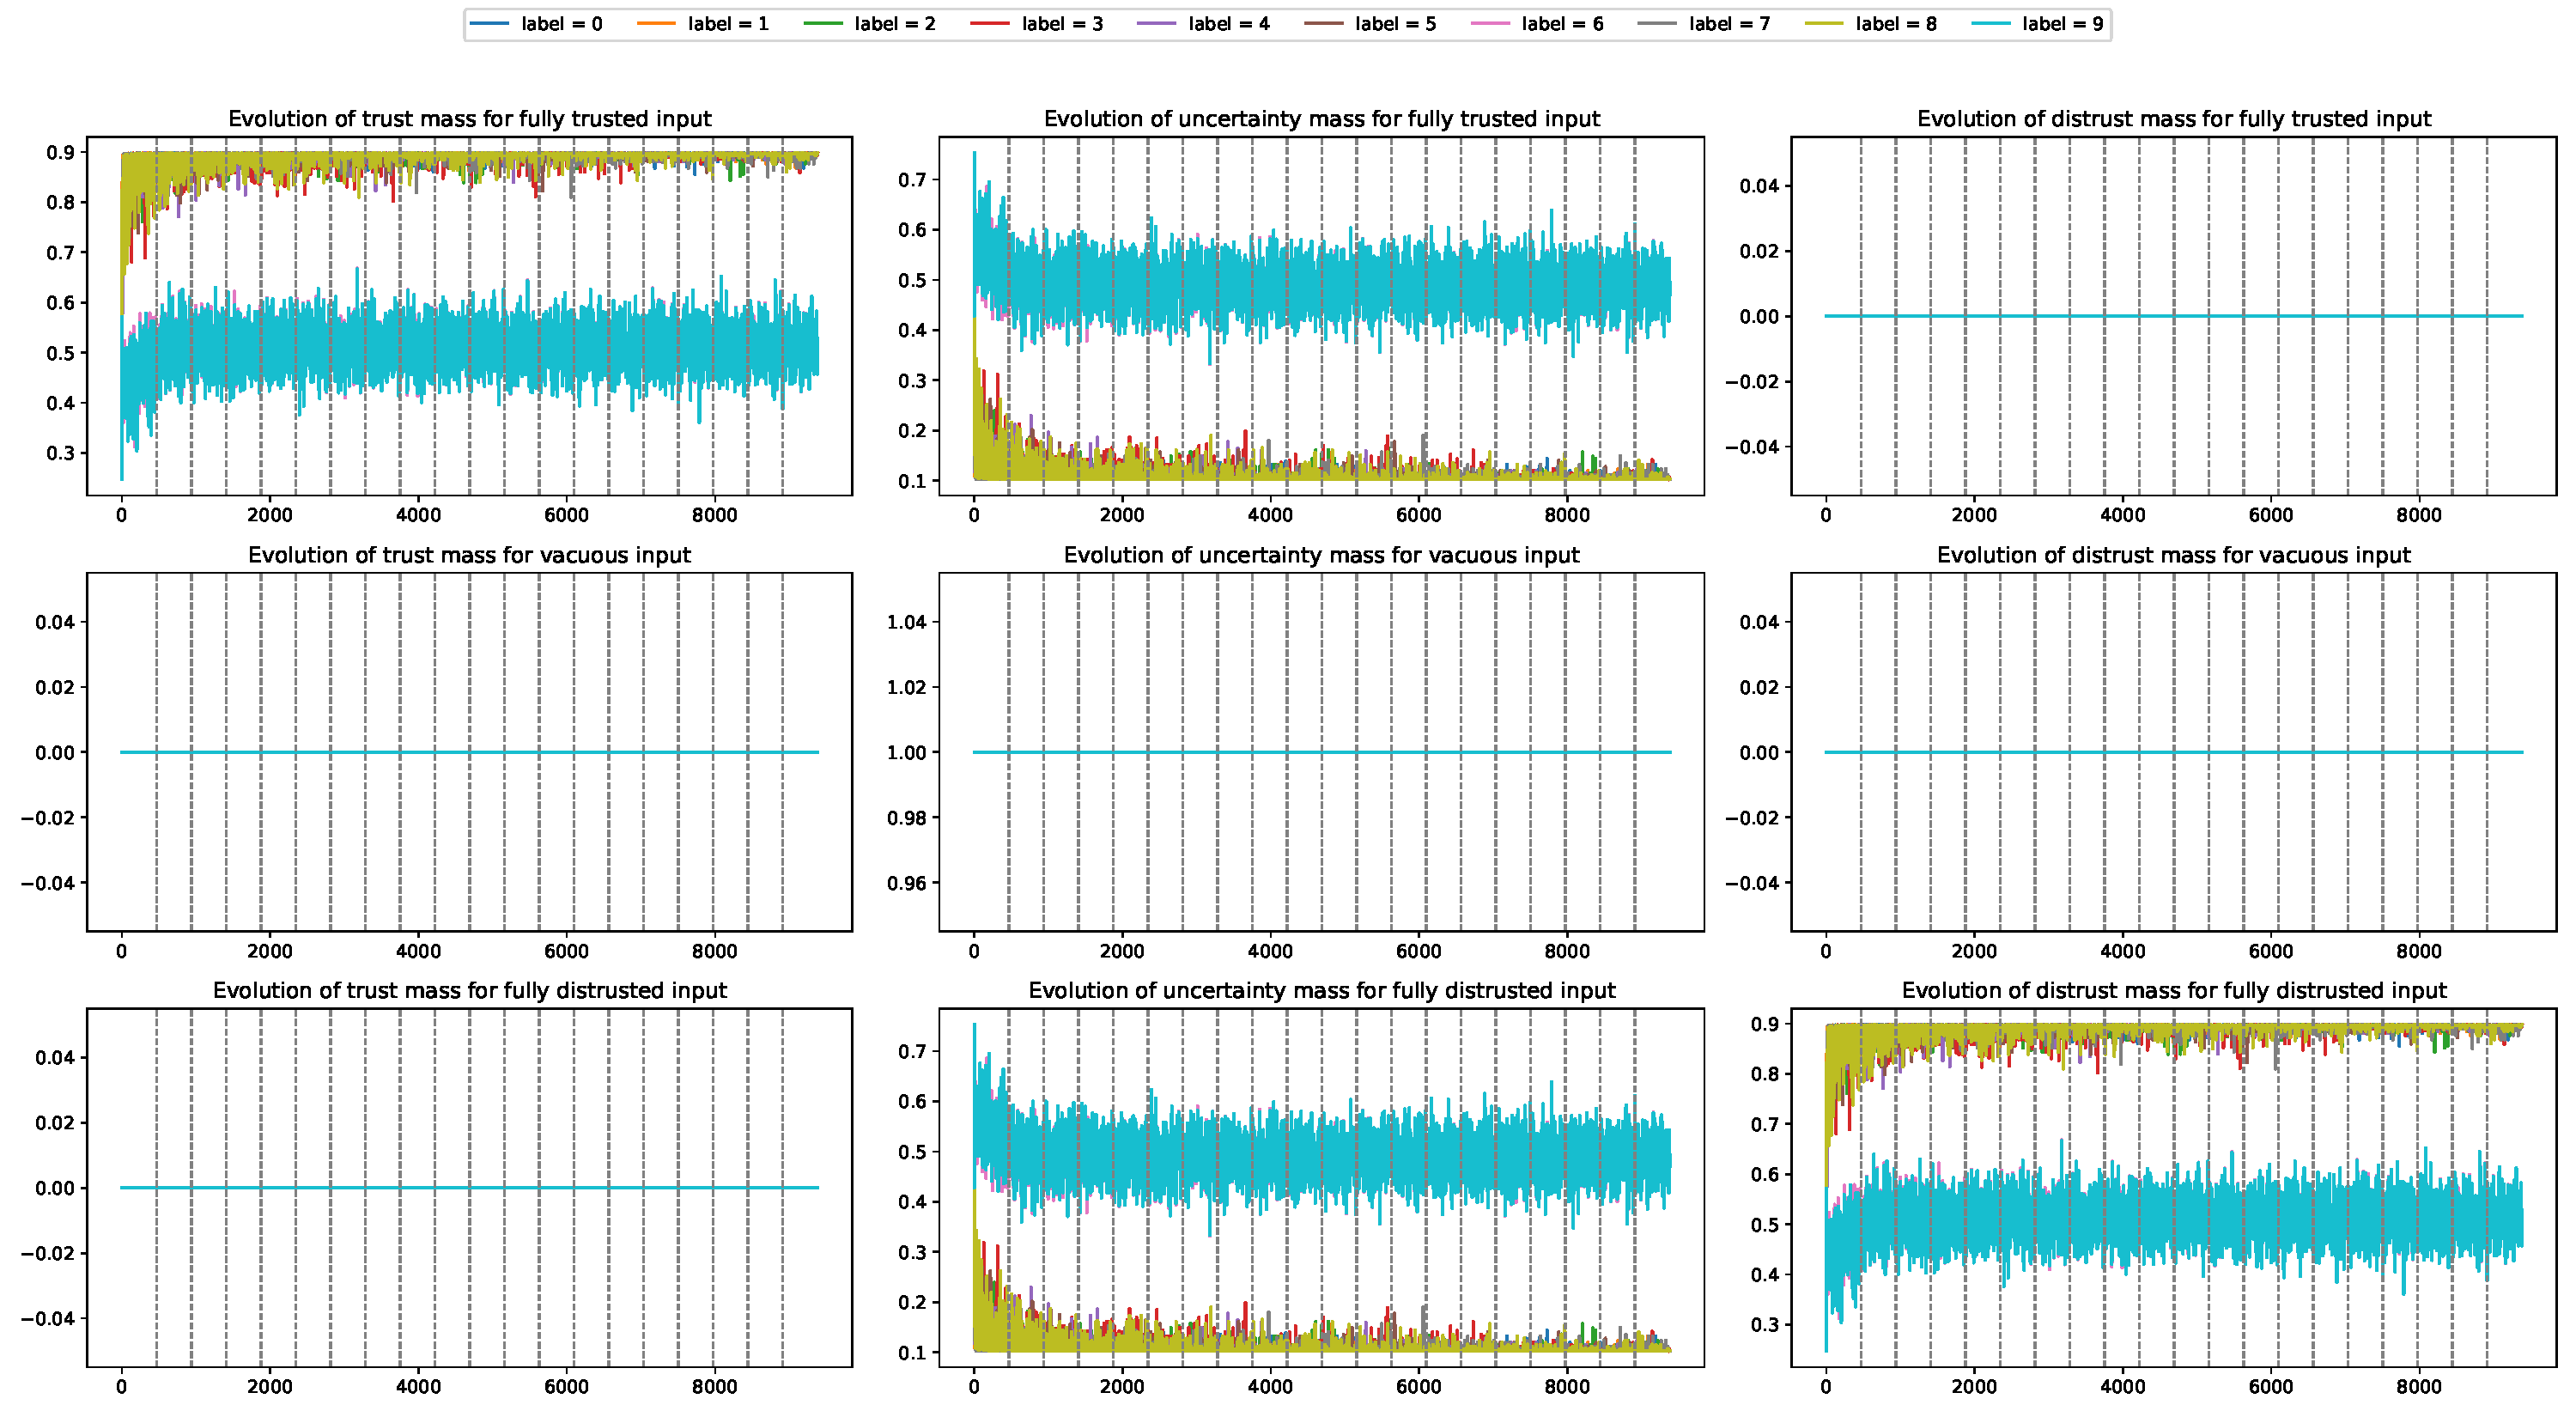
\includegraphics[width=\textwidth]{plots_v2/MNIST/poisoned/plot_ptas-128-t-t-ps1.pdf}
  \caption{1 pixel}
\end{figure}
\begin{figure}[H]
  \centering
  \includegraphics[width=\textwidth]{plots_v2/MNIST/poisoned/plot_ptas-128-t-t-ps4.pdf}
  \caption{4×4 pixels}
\end{figure}
\begin{figure}[H]
  \centering
  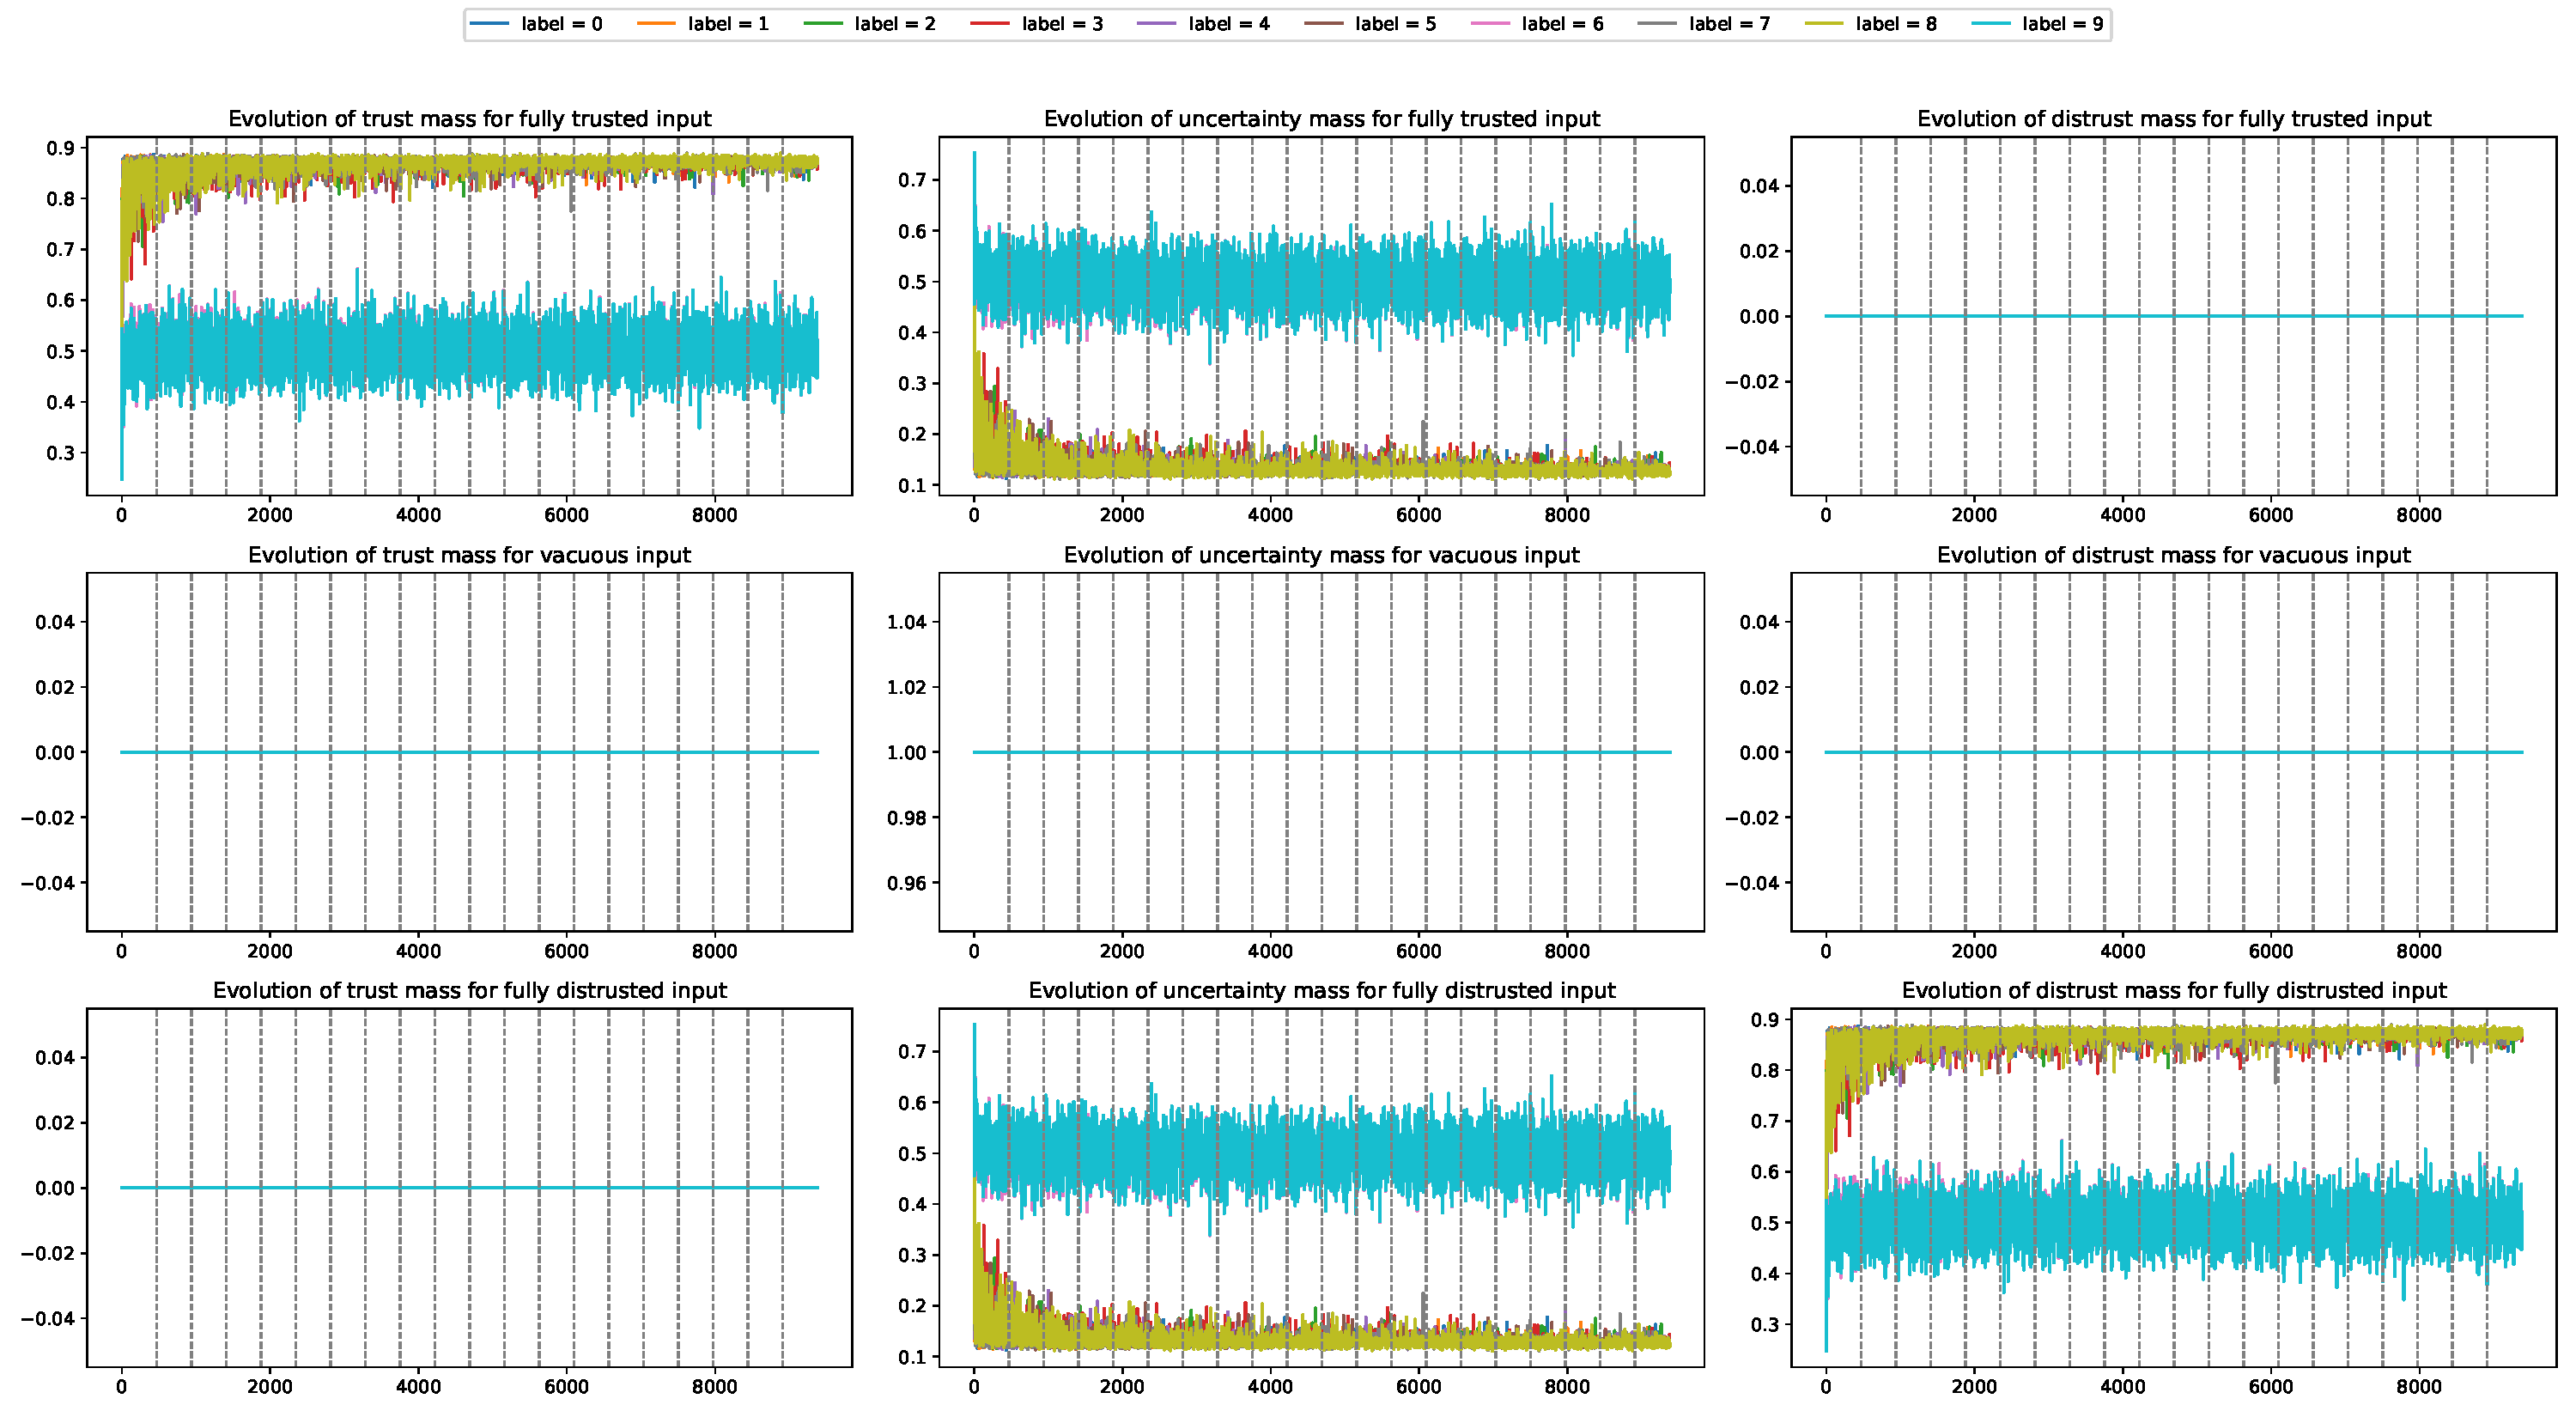
\includegraphics[width=\textwidth]{plots_v2/MNIST/poisoned/plot_ptas-128-t-t-ps10.pdf}
  \caption{10×10 pixels}
\end{figure}
\begin{figure}[H]
  \centering
  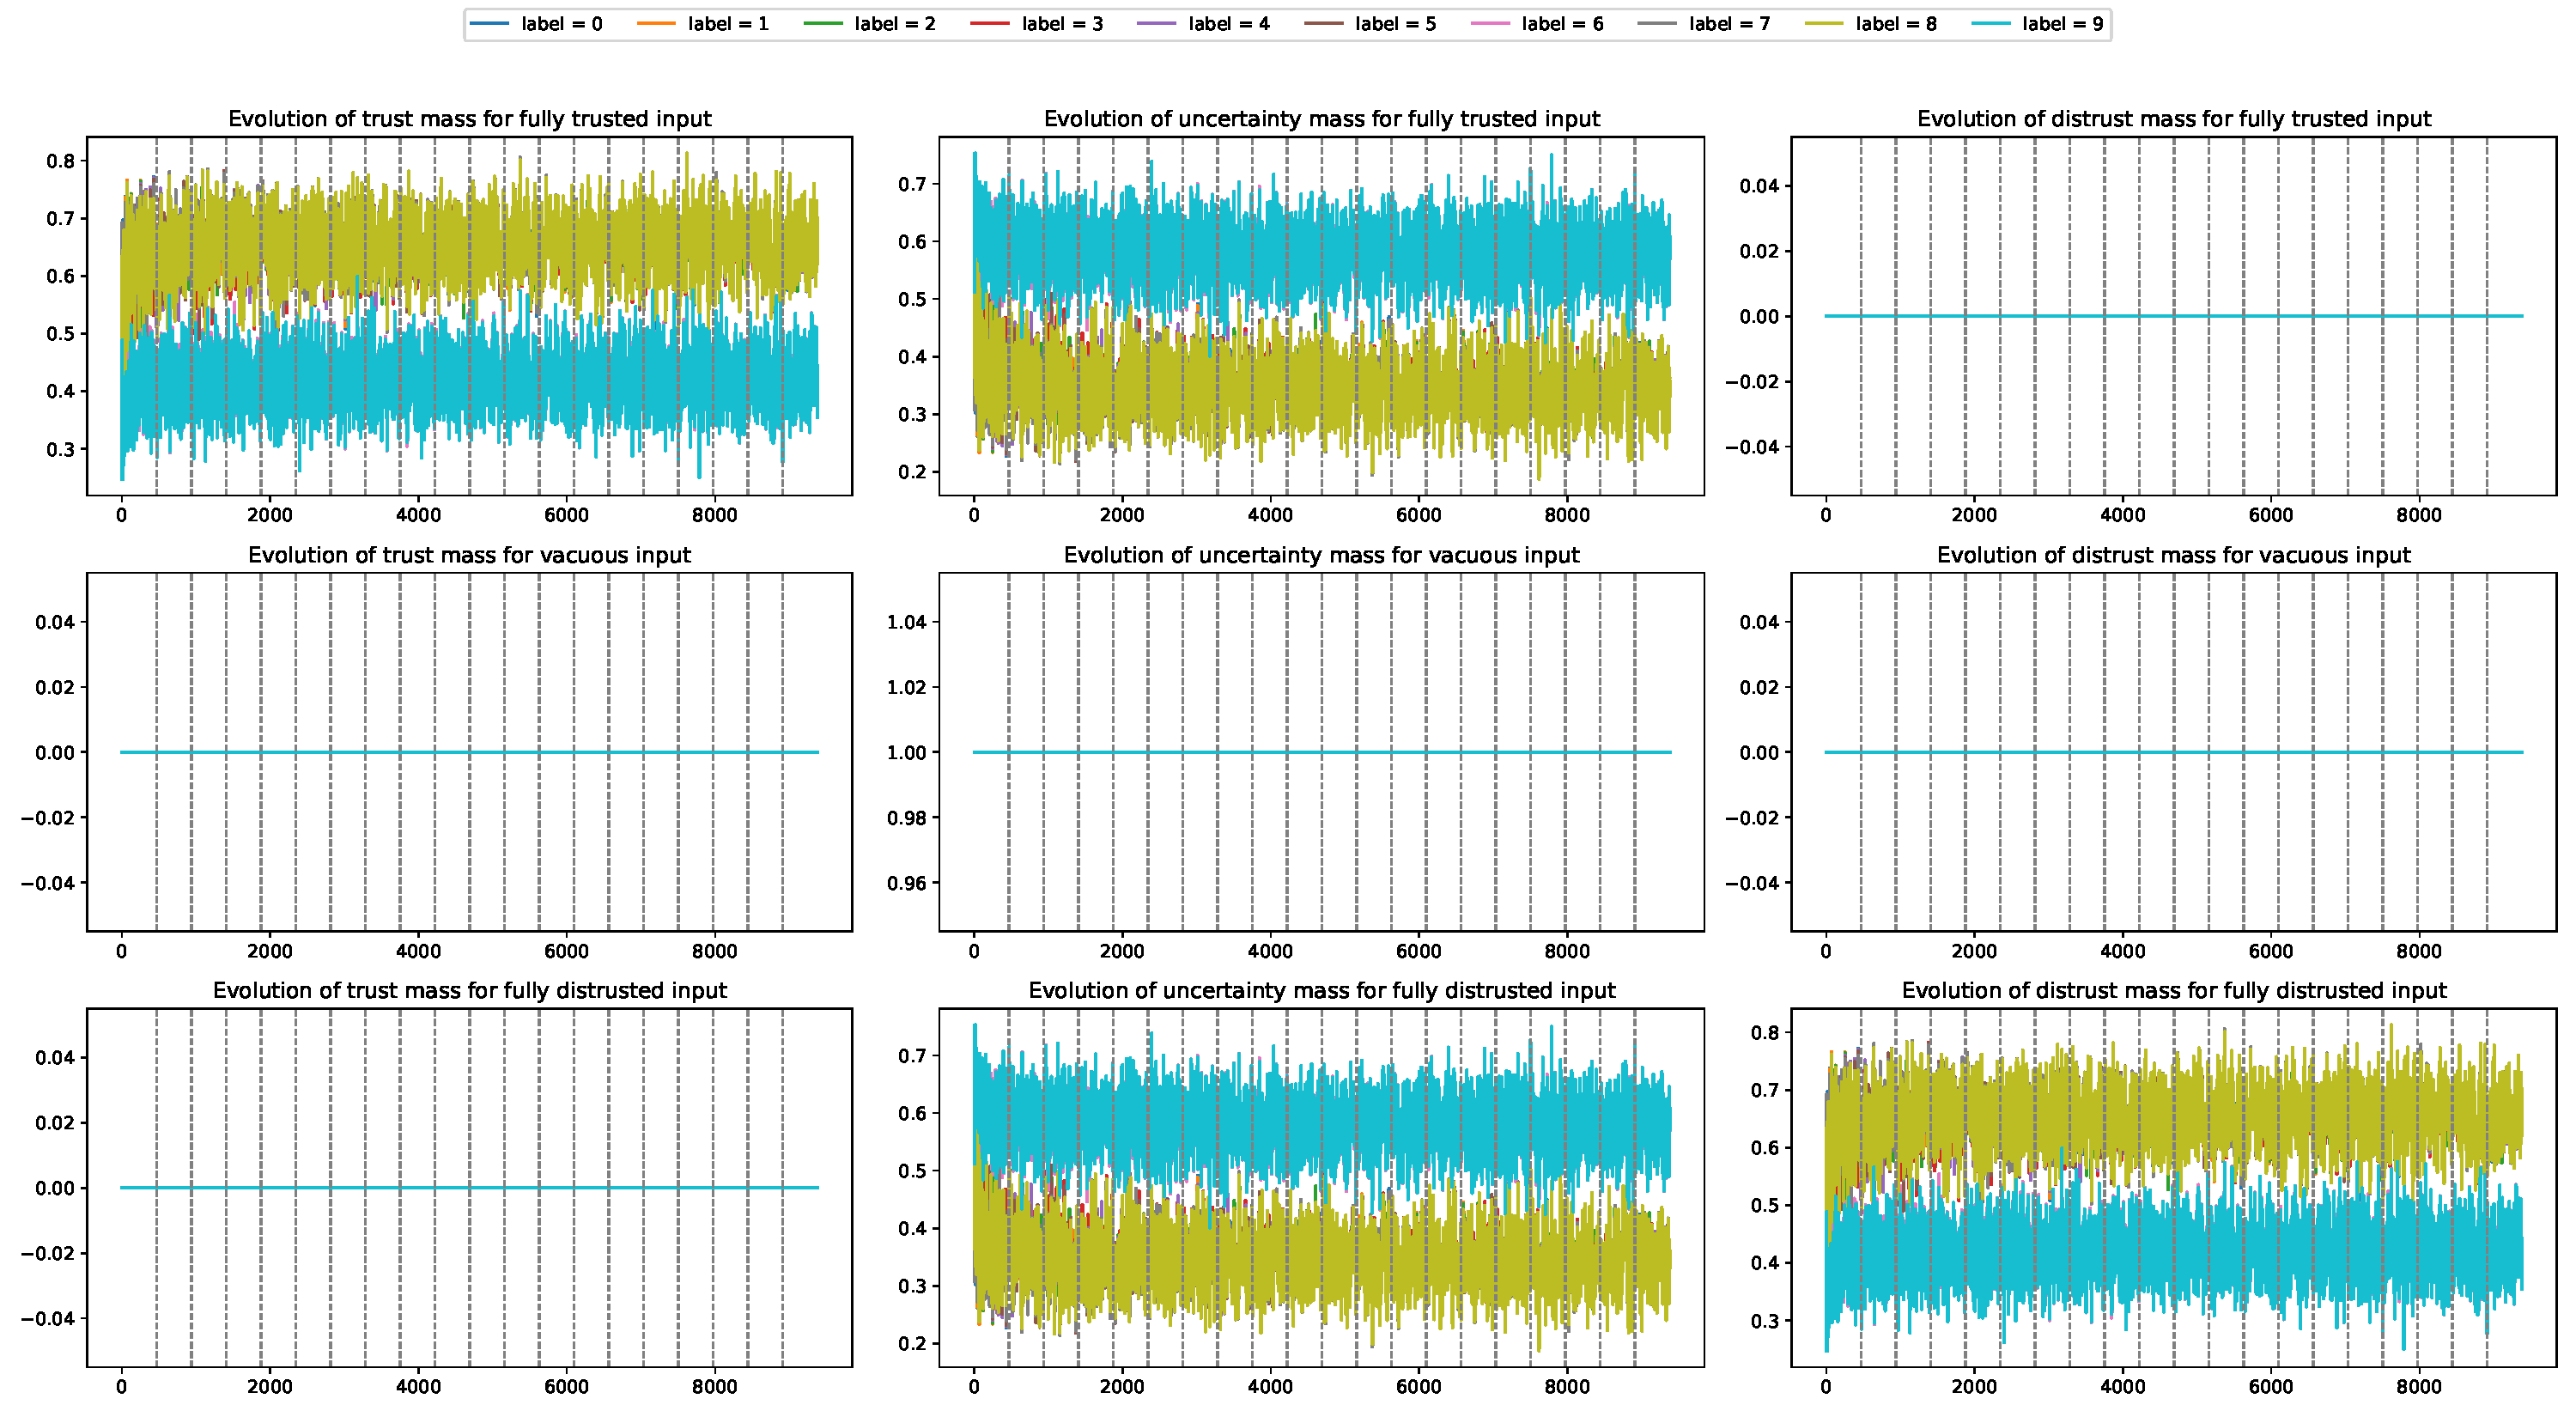
\includegraphics[width=\textwidth]{plots_v2/MNIST/poisoned/plot_ptas-128-t-t-ps27.pdf}
  \caption{27×27 pixels}
\end{figure}
\subsection{Plots for the Comparative Trust Evaluation (\cref{exp:4})}\label{sec:resexp4}
\begin{figure}[H]
  \centering
  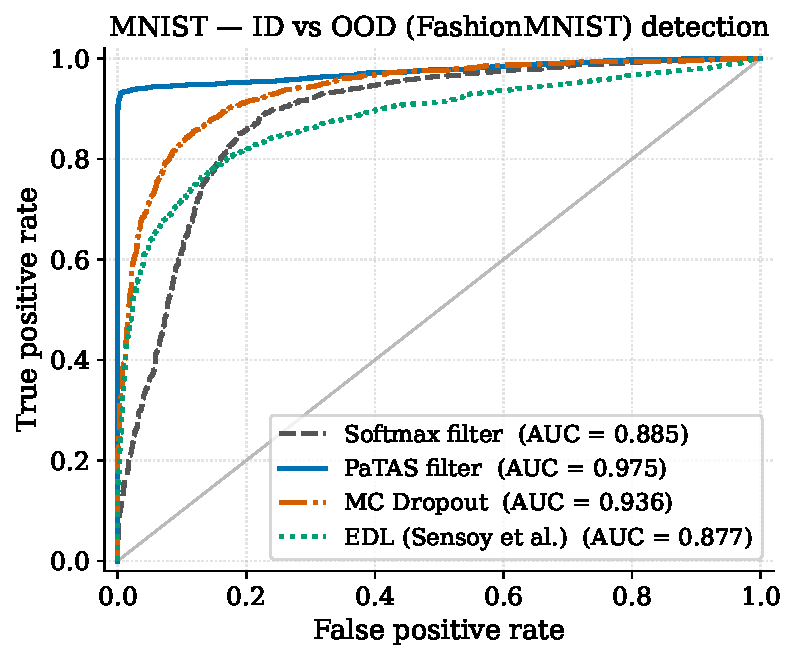
\includegraphics[width=0.62\textwidth]{plots_v2/exp4/roc_ood_mnist.pdf}
  \caption{Out-of-distribution detection ROC (MNIST in-distribution vs.\ Fashion-MNIST OOD): each method's own score as the discriminator. Curves and legend AUC values are from a single representative evaluation seed; \cref{tab:comparative} reports mean $\pm$ std over three seeds.}
\end{figure}
\begin{figure}[H]
  \centering
  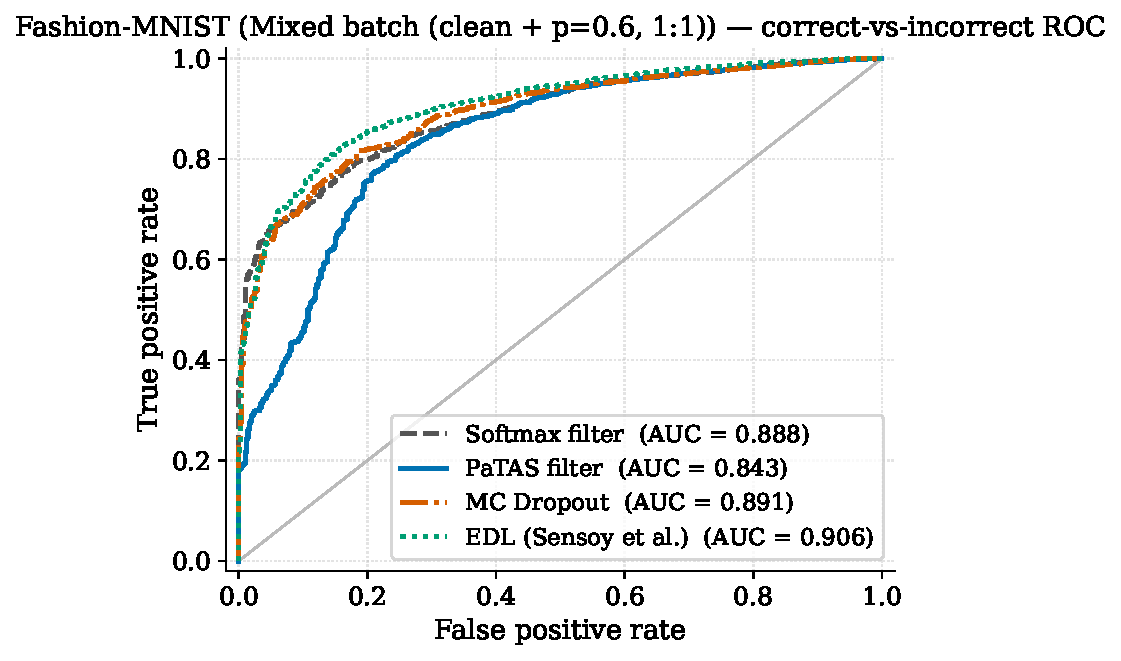
\includegraphics[width=0.62\textwidth]{plots_v2/exp4/roc_mixed_fashion.pdf}
  \caption{Correct-vs-incorrect ROC on the Fashion-MNIST mixed batch (clean + corrupted inputs pooled 1:1), single representative evaluation seed.}
\end{figure}
\begin{figure}[H]
  \centering
  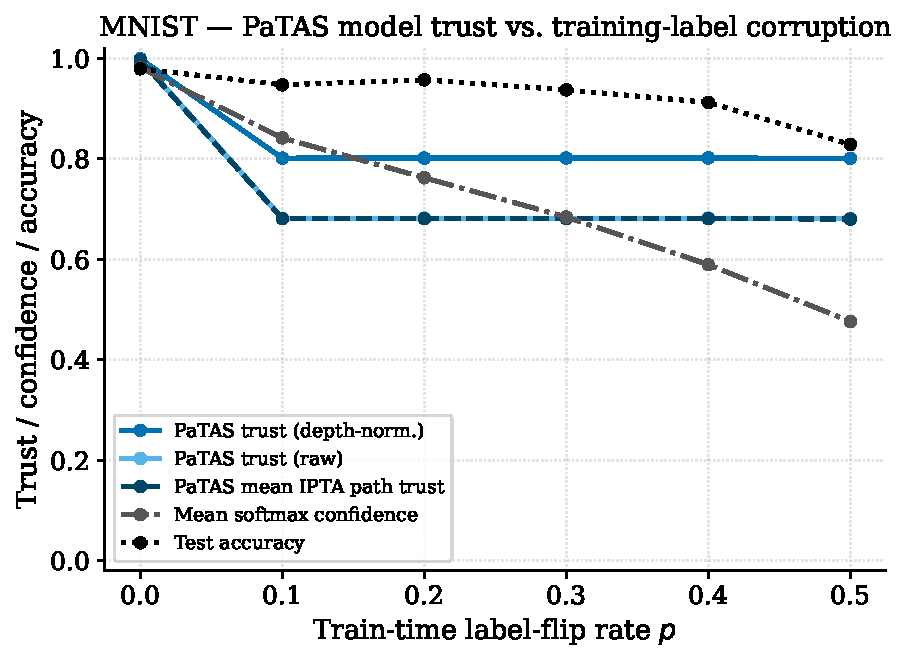
\includegraphics[width=0.62\textwidth]{plots_v2/exp4/model_trust_vs_labelnoise.pdf}
  \caption{Training-quality audit (\cref{tab:audit}): PaTAS model-side trust, mean softmax confidence, and test accuracy as functions of the train-time label-flip rate $p$. The depth-normalized curve rescales the committed mass $b+d$ of the aggregated opinion to $(b+d)^{1/L}$, with $L$ the number of trust-propagation layers, making trust comparable across network depths. Trust drops as a tripwire at any non-zero rate without using test data; confidence tracks severity but requires a clean labelled test set.}
\end{figure}


\end{document}

